\chapter{Markov Chains and MCMC: The Biased Random Walker}\label{ch:09}
\providecommand{\NineAOscN}{}\renewcommand{\NineAOscN}{50\,000}
\providecommand{\NineAOscChi}{}\renewcommand{\NineAOscChi}{75.9}
\providecommand{\NineAOscBins}{}\renewcommand{\NineAOscBins}{80}
\providecommand{\NineAOscMeanSq}{}\renewcommand{\NineAOscMeanSq}{0.501}
\providecommand{\NineATwoMeanTime}{}\renewcommand{\NineATwoMeanTime}{0.489}
\providecommand{\NineATwoSqTime}{}\renewcommand{\NineATwoSqTime}{0.357}
\providecommand{\NineATwoLowTime}{}\renewcommand{\NineATwoLowTime}{0.205}
\providecommand{\NineATwoMeanEns}{}\renewcommand{\NineATwoMeanEns}{0.489}
\providecommand{\NineATwoSqEns}{}\renewcommand{\NineATwoSqEns}{0.318}
\providecommand{\NineATwoLowEns}{}\renewcommand{\NineATwoLowEns}{0.102}
\providecommand{\NineATwoKappa}{}\renewcommand{\NineATwoKappa}{0.05}
\providecommand{\NineAIslTwoThree}{}\renewcommand{\NineAIslTwoThree}{0.375}
\providecommand{\NineAIslTwoFour}{}\renewcommand{\NineAIslTwoFour}{0.125}
\providecommand{\NineAIslTwoFive}{}\renewcommand{\NineAIslTwoFive}{0.5}
\providecommand{\NineAIslThreeTwo}{}\renewcommand{\NineAIslThreeTwo}{0.125}
\providecommand{\NineAIslThreeThree}{}\renewcommand{\NineAIslThreeThree}{0.1094}
\providecommand{\NineAIslThreeFour}{}\renewcommand{\NineAIslThreeFour}{0.4031}
\providecommand{\NineAIslThreeFive}{}\renewcommand{\NineAIslThreeFive}{0.1125}
\providecommand{\NineAIslThreeSix}{}\renewcommand{\NineAIslThreeSix}{0.25}
\providecommand{\NineAIslTVThirteen}{}\renewcommand{\NineAIslTVThirteen}{0.048}
\providecommand{\NineAIslTVNinetyNine}{}\renewcommand{\NineAIslTVNinetyNine}{1.5\times10^{-6}}
\providecommand{\NineAIslMaxDev}{}\renewcommand{\NineAIslMaxDev}{0.0025}
\providecommand{\NineAIslDays}{}\renewcommand{\NineAIslDays}{100\,000}
\providecommand{\NineAIslWalkers}{}\renewcommand{\NineAIslWalkers}{20\,000}
\providecommand{\NineAIslLamTwo}{}\renewcommand{\NineAIslLamTwo}{0.887}
\providecommand{\NineAWLamTwo}{}\renewcommand{\NineAWLamTwo}{0.6}
\providecommand{\NineAWLamThree}{}\renewcommand{\NineAWLamThree}{0.1}
\providecommand{\NineAWSlope}{}\renewcommand{\NineAWSlope}{-0.5108}
\providecommand{\NineAWLnLam}{}\renewcommand{\NineAWLnLam}{-0.5108}
\providecommand{\NineAWDelta}{}\renewcommand{\NineAWDelta}{0.3}
\providecommand{\NineAWTVTen}{}\renewcommand{\NineAWTVTen}{0.0036}
\providecommand{\NineAWTVTenPred}{}\renewcommand{\NineAWTVTenPred}{0.0036}
\providecommand{\NineAWTVTwenty}{}\renewcommand{\NineAWTVTwenty}{2.19\times10^{-5}}
\providecommand{\NineAWMCFloor}{}\renewcommand{\NineAWMCFloor}{1.2\times10^{-3}}
\providecommand{\NineAWWalkers}{}\renewcommand{\NineAWWalkers}{200\,000}
\providecommand{\NineAWTwoSunThree}{}\renewcommand{\NineAWTwoSunThree}{0.544}
\providecommand{\NineAWTwoSunSix}{}\renewcommand{\NineAWTwoSunSix}{0.5732}
\providecommand{\NineACoupIndTen}{}\renewcommand{\NineACoupIndTen}{0.018}
\providecommand{\NineACoupDoeTen}{}\renewcommand{\NineACoupDoeTen}{0.0046}
\providecommand{\NineACoupTVTen}{}\renewcommand{\NineACoupTVTen}{0.0036}
\providecommand{\NineACoupBoundTen}{}\renewcommand{\NineACoupBoundTen}{0.0235}
\providecommand{\NineACoupWalkers}{}\renewcommand{\NineACoupWalkers}{200\,000}
\providecommand{\NineAErgRainTau}{}\renewcommand{\NineAErgRainTau}{2.222}
\providecommand{\NineAErgRainFrac}{}\renewcommand{\NineAErgRainFrac}{0.1665}
\providecommand{\NineAErgRainGap}{}\renewcommand{\NineAErgRainGap}{6.007}
\providecommand{\NineAErgRainErr}{}\renewcommand{\NineAErgRainErr}{5.6\times10^{-4}}
\providecommand{\NineAErgLong}{}\renewcommand{\NineAErgLong}{10^6}
\providecommand{\NineAErgWeatherTau}{}\renewcommand{\NineAErgWeatherTau}{0.429}
\providecommand{\NineAErgStickyTau}{}\renewcommand{\NineAErgStickyTau}{5.667}
\providecommand{\NineAErgWeatherMeas}{}\renewcommand{\NineAErgWeatherMeas}{0.1044}
\providecommand{\NineAErgWeatherPred}{}\renewcommand{\NineAErgWeatherPred}{0.105}
\providecommand{\NineAErgStickyMeas}{}\renewcommand{\NineAErgStickyMeas}{1.282}
\providecommand{\NineAErgStickyPred}{}\renewcommand{\NineAErgStickyPred}{1.259}
\providecommand{\NineAErgStickyMean}{}\renewcommand{\NineAErgStickyMean}{0.6657}
\providecommand{\NineAErgDieTau}{}\renewcommand{\NineAErgDieTau}{1.9}
\providecommand{\NineAErgDieLam}{}\renewcommand{\NineAErgDieLam}{0.9}
\providecommand{\NineAErgDieErr}{}\renewcommand{\NineAErgDieErr}{0.0744}
\providecommand{\NineAErgFairErr}{}\renewcommand{\NineAErgFairErr}{0.055}
\providecommand{\NineAErgChains}{}\renewcommand{\NineAErgChains}{4000}
\providecommand{\NineADiffVarHundred}{}\renewcommand{\NineADiffVarHundred}{100.7}
\providecommand{\NineADiffVarThousand}{}\renewcommand{\NineADiffVarThousand}{1014}
\providecommand{\NineADiffWalkers}{}\renewcommand{\NineADiffWalkers}{20\,000}
\providecommand{\NineAARMeanForty}{}\renewcommand{\NineAARMeanForty}{0.29}
\providecommand{\NineAARMeanFortyPred}{}\renewcommand{\NineAARMeanFortyPred}{0.296}
\providecommand{\NineAARVarEnd}{}\renewcommand{\NineAARVarEnd}{1.016}
\providecommand{\NineAARVarEndPred}{}\renewcommand{\NineAARVarEndPred}{1}
\providecommand{\NineAARMeanEnd}{}\renewcommand{\NineAARMeanEnd}{-0.005}
\providecommand{\NineAMLEn}{}\renewcommand{\NineAMLEn}{1000}
\providecommand{\NineAMLERep}{}\renewcommand{\NineAMLERep}{2000}
\providecommand{\NineAMLEzSd}{}\renewcommand{\NineAMLEzSd}{1.013}
\providecommand{\NineAMLEzMean}{}\renewcommand{\NineAMLEzMean}{0.01}
\providecommand{\NineAMLESS}{}\renewcommand{\NineAMLESS}{0.624}
\providecommand{\NineAMLEseSS}{}\renewcommand{\NineAMLEseSS}{0.021}
\providecommand{\NineAMLESC}{}\renewcommand{\NineAMLESC}{0.197}
\providecommand{\NineAMLEseSC}{}\renewcommand{\NineAMLEseSC}{0.017}
\providecommand{\NineAMLESR}{}\renewcommand{\NineAMLESR}{0.18}
\providecommand{\NineAMLEseSR}{}\renewcommand{\NineAMLEseSR}{0.017}
\providecommand{\NineAMLECS}{}\renewcommand{\NineAMLECS}{0.295}
\providecommand{\NineAMLEseCS}{}\renewcommand{\NineAMLEseCS}{0.025}
\providecommand{\NineAMLECC}{}\renewcommand{\NineAMLECC}{0.705}
\providecommand{\NineAMLEseCC}{}\renewcommand{\NineAMLEseCC}{0.025}
\providecommand{\NineAMLECR}{}\renewcommand{\NineAMLECR}{0}
\providecommand{\NineAMLEseCR}{}\renewcommand{\NineAMLEseCR}{0}
\providecommand{\NineAMLERS}{}\renewcommand{\NineAMLERS}{0.664}
\providecommand{\NineAMLEseRS}{}\renewcommand{\NineAMLEseRS}{0.04}
\providecommand{\NineAMLERC}{}\renewcommand{\NineAMLERC}{0}
\providecommand{\NineAMLEseRC}{}\renewcommand{\NineAMLEseRC}{0}
\providecommand{\NineAMLERR}{}\renewcommand{\NineAMLERR}{0.336}
\providecommand{\NineAMLEseRR}{}\renewcommand{\NineAMLEseRR}{0.04}
\providecommand{\NineAMLEnS}{}\renewcommand{\NineAMLEnS}{518}
\providecommand{\NineAMLEnC}{}\renewcommand{\NineAMLEnC}{342}
\providecommand{\NineAMLEnR}{}\renewcommand{\NineAMLEnR}{140}
\providecommand{\NineARetHalf}{}\renewcommand{\NineARetHalf}{0.9916}
\providecommand{\NineARetSix}{}\renewcommand{\NineARetSix}{0.801}
\providecommand{\NineARetHalfPred}{}\renewcommand{\NineARetHalfPred}{0.992}
\providecommand{\NineARetSumHalf}{}\renewcommand{\NineARetSumHalf}{49.5}
\providecommand{\NineARetSumSix}{}\renewcommand{\NineARetSumSix}{4}
\providecommand{\NineARetWalkers}{}\renewcommand{\NineARetWalkers}{10\,000}
\providecommand{\NineARetSteps}{}\renewcommand{\NineARetSteps}{10\,000}
\providecommand{\NineARetStirTen}{}\renewcommand{\NineARetStirTen}{0.9876}
\providecommand{\NineACycJ}{}\renewcommand{\NineACycJ}{0.1333}
\providecommand{\NineACycLam}{}\renewcommand{\NineACycLam}{0.4}
\providecommand{\NineACycTVTen}{}\renewcommand{\NineACycTVTen}{7.0\times10^{-5}}
\section*{Where this chapter is going}
\label{9a:sec:roadmap}

By the end of \cref{ch:05} every inference problem had the same shape. The data $\data$ have
been observed, the parameters $\params$ are the possible explanations, and Bayes' theorem
gives the posterior $p(\params\given\data)\propto\Like(\params)\,p(\params)$, the likelihood
times the prior. We can evaluate the right-hand side at any $\params$ we like. What we cannot
do, once $\params$ has more than two or three components, is integrate it: the evidence
$Z=p(\data)$, every posterior mean, every marginal and every credible interval is an integral
over the whole parameter space. A grid of 100 points per axis already needs $10^{12}$
evaluations for six cosmological parameters.

There is a way round the integrals, and the book has used it since \cref{ch:01}: a large
sample from a distribution \emph{is} the distribution, for every practical purpose. Histogram
the sample and you have the density; average a function over the sample and you have its
expectation; ignore a column and you have marginalised over that parameter
\srcref{Kruschke}{§7.1}. So the question becomes: how do we draw a large sample from a
distribution that we can only evaluate, up to a constant, one point at a time?

Sometimes nature answers it for us. An oscillator of fixed energy, looked at at random
instants, hands us a sample of its phase-space orbit with no effort at all, because its
motion carries it over the orbit at exactly the right rate. That trick fails as soon as the
system has more than a few degrees of freedom, and it does not exist for a posterior, which
has no motion. So we build the motion ourselves: a random walker that hops from point to
point, remembering only where it is now, with hopping rules chosen so that the fraction of
time it spends anywhere equals the probability we want. Such a walker is a Markov chain.
Three facts make it work: the target distribution is \emph{stationary} (a walker distributed
according to it stays so), the walker \emph{forgets where it started} (every starting
distribution converges to the same stationary one, at a rate we can compute), and
\emph{time averages equal ensemble averages} (the ergodic theorem), so one long walk is as good
as many independent draws, only noisier. Metropolis--Hastings then gives a recipe for the
hopping rule for \emph{any} target, which is the biased random walker;
diagnostics tell us when a finite walk can be trusted, and the same machine produces the
posterior of cosmological parameters from a CMB power spectrum
(\cref{9a:fig:roadmap}).

In the pipeline of the book (physical model $\to$ field $\to$ what matters $\to$ summary
$\to$ sampling distribution $\to$ inference) this chapter is the last arrow. \Cref{ch:07,ch:08}
produced the sampling distribution of a summary, $p(\Chat\given\params)$; here that likelihood
becomes a cloud of posterior samples from which every constraint is read off.

\begin{figure}[htbp]
\centering
\begin{tikzpicture}[
  bx/.style={draw=accent,thick,rounded corners=2pt,fill=ideabg,font=\small,
             minimum height=11mm,align=center,text width=30mm},
  gb/.style={bx,draw=tangentgreen!80!black},
  rb/.style={bx,draw=bdryred!80!black},
  flow/.style={->,thick,accent}]
  \node[bx] (tgt) at (0,0)     {target $\pi(\params)\propto\Like\,p(\params)$\\ known up to $Z$};
  \node[gb] (osc) at (4.4,1.1) {a motion does the sampling\\ (oscillator,\\ \mbox{uniform time})};
  \node[rb] (no)  at (4.4,-1.1){no motion to use\\ (many particles, posteriors)};
  \node[bx] (mc)  at (8.8,-1.1){random walker with\\ memory of one step};
  \node[bx] (st)  at (8.8,-3.3){$\pi$ stationary; start\\ forgotten as $\abs{\lambda_2}^t$};
  \node[bx] (er)  at (4.4,-3.3){time average $=$\\ ensemble average};
  \node[bx] (mh)  at (0,-3.3)  {Metropolis--Hastings:\\ a hopping rule for any $\pi$};
  \node[bx] (app) at (0,-5.5)  {diagnostics, then\\ CMB parameters};
  \draw[flow] (tgt.east) -- ++(0.5,0) |- (osc.west);
  \draw[flow] (tgt.east) -- ++(0.5,0) |- (no.west);
  \draw[flow] (no) -- (mc);
  \draw[flow] (mc) -- (st);
  \draw[flow] (st) -- (er);
  \draw[flow] (er) -- (mh);
  \draw[flow] (mh) -- (app);
  \draw[flow,dashed,softgray] (osc.east) -- (6.4,1.1) -- (6.4,-2.15) -- (5.5,-2.15) -- (5.5,-2.75);
\end{tikzpicture}
\caption{The route of the chapter. A distribution we can evaluate but not integrate is
sampled directly when some motion already walks over it at the right rate (green), which
is the oscillator. When there is no such motion (red) we construct a random walk whose
long-run time fractions are the target; the dashed line marks that the oscillator and the
Markov chain rest on the same property, equality of time and ensemble averages.}
\label{9a:fig:roadmap}
\end{figure}

\section{When the motion samples for us: the oscillator}
\label{9a:sec:oscillator}

The easiest sampling problem in physics has already been solved in \cref{ch:01}, and it is
worth seeing again why it was so easy, because the reason is exactly what a Markov chain will
have to reproduce by force.

\paragraph{The question.}
A mass on a spring with fixed energy moves as $x(t)=A\cos\omega t$, $p(t)=-m\omega
A\sin\omega t$. We look at it at a randomly chosen instant. Where do we find it?
At this energy the possible states are the points $(x,p)$ of the energy ellipse in phase
space, so the ellipse is the sample space. The motion passes each of its points once per
period, so a random instant picks a random point of it. To find the distribution of position,
then, we histogram $x$ for a large set of random instants. Before doing so, recall the chain
of \cref{1b:ex:arcsine} that predicts what the histogram must look like.

\emph{Uniform time.} ``A randomly chosen instant'' is a sampling prescription: every instant
of one period $T=2\pi/\omega$ is equally likely, $P(t)\,\dd t=\dd t/T$, which is
\eqref{1b:eq:uniform-time}.

\emph{From time to position.} The position $x=A\cos\omega t$ changes at the speed
$\abs{\dd x/\dd t}=\abs v=\omega\sqrt{A^2-x^2}$, so the mass spends a time $\dd t=\dd x/\abs v$
in the interval $[x,x+\dd x]$, and it passes through that interval twice per period (once
going out, once coming back). Adding the two visits,
\begin{equation}
  P(x)\,\dd x=2\times\frac1T\,\frac{\dd x}{\abs v}=\frac{2}{T}\,\frac{\dd x}{\omega\sqrt{A^2-x^2}},
  \qquad\text{so}\qquad
  P(x)=\frac{1}{\pi\sqrt{A^2-x^2}},\qquad \abs{x}<A,
  \label{9a:eq:arcsine}
\end{equation}
the arcsine law, using $T\omega=2\pi$ in the last step. It is large near the turning points
because the mass is slow there.

\emph{The same law with no clock.} Suppose we did not know that the instant is uniform, and
asked instead which states of the energy shell $E<H<E+\Delta E$ are equally likely (the
microcanonical ensemble). The vertical strip of phase space over $[x,x+\dd x]$ cuts the shell
in two thin patches, at $p_+$ and $p_-$. Each patch has width $\dd x$ and height $\Delta p$,
and the height follows from $H=p^2/2m+\tfrac12m\omega^2x^2$: at fixed $x$, $\dd H=(p/m)\,\dd p$,
so $\Delta p=\Delta E/\abs v$. The shell area inside the strip is therefore
$2\,\dd x\,\Delta E/\abs v$, again proportional to $\dd x/\abs v$, and normalising gives
\eqref{9a:eq:arcsine} a second time.

\emph{Why the two agree.} The first route averages over the instants of one trajectory; the
second averages over all the states of the shell. They give the same answer because the time
the motion spends in a patch of the shell, $\dd x/\abs v$, is proportional to the patch's
area. Time average equals ensemble average, and that equality is what \emph{ergodic} will
mean below.

\paragraph{The sampler is one line.}
In units $m=\omega=1$ the script draws a uniform phase $\theta=\omega t$ and lets the motion
do the rest.
\pyfile[firstline=30,lastline=39,firstnumber=30]{code/ch09/01_oscillator_phase_space.py}{The oscillator: uniform phases, then the deterministic map to the orbit}
Line 31 is the only random line, and it chooses \emph{when} we look. Lines 32--33 are the
equation of motion: they carry the chosen instant to its point $(x,p)$ of the orbit, the
sampled element of the sample space. Lines 36--39 compare the histogram with
\eqref{9a:eq:arcsine} bin by bin, using the exact bin probabilities
$F(x_{k+1})-F(x_k)$ with $F(x)=\tfrac12+\tfrac1\pi\arcsin(x/A)$ (Method~1 of \cref{1b:ex:arcsine}).
With $N=\NineAOscN$ phases the mismatch is $\chi^2=\NineAOscChi$ over $\NineAOscBins$ bins,
as it should be for a correct law (a $\chi^2$ variable with $\nu$ degrees of freedom has mean
$\nu$ and standard deviation $\sqrt{2\nu}\approx13$ here), and the average of $x^2$ over the
sampled instants is $\NineAOscMeanSq\,A^2$ against the exact $A^2/2$
(\cref{9a:fig:oscillator}).

\begin{figure}[htbp]
\centering
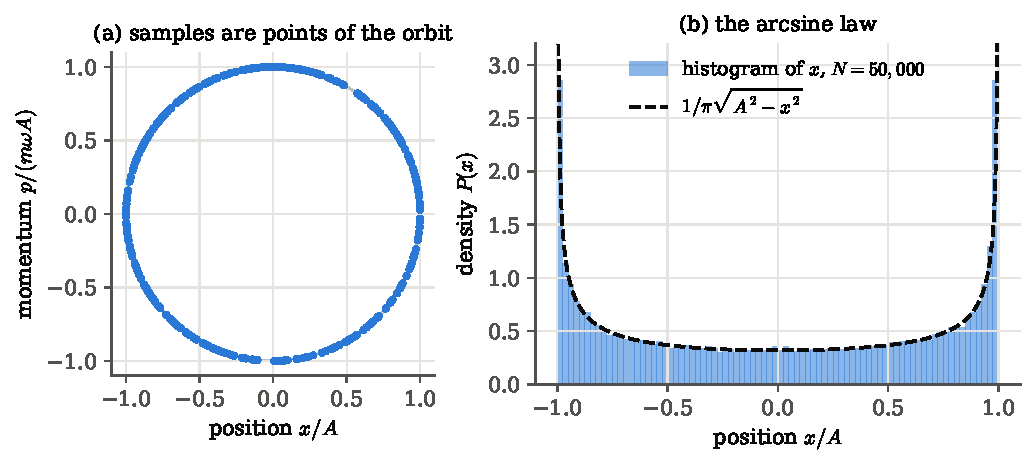
\includegraphics[width=\linewidth]{figures/ch09/oscillator_phase_space.pdf}
\caption{(a) Four hundred random instants, drawn as the phase-space points the oscillator
occupies at those instants: every sample lies on the energy circle (scaled units), which is
the whole sample space. (b) The positions of $5\times10^4$ such instants follow the arcsine
law, piling up at the turning points where the mass moves slowly.}
\label{9a:fig:oscillator}
\end{figure}

\paragraph{Why it was so easy.}
Two things happened together. The equation of motion visits every state of the sample space,
and it spends in each part of it a time proportional to that part's probability. So drawing
from the distribution reduces to drawing a uniform time, which any random-number generator
does. In the language of statistical mechanics the agreement of the two derivations of
\eqref{9a:eq:arcsine}, uniform time and microcanonical shell area, says that the average of any
quantity over one long trajectory equals its average over the ensemble of all states of the
energy shell. That property has a name.

\begin{keyidea}[Ergodicity: time average $=$ ensemble average]
A dynamics is \newterm{ergodic} on a set of states if, for every function $g$ of the state,
the average of $g$ along one long trajectory equals the average of $g$ over the set with the
ensemble's probabilities. Then one trajectory, looked at at random times, is a sample of the
ensemble. A Markov chain is useful for exactly this reason.
\end{keyidea}

\paragraph{The hidden assumption, and a counterexample.}
For one oscillator the property is automatic: the energy shell is a single closed curve and
the orbit is all of it. Nothing guarantees it in general, and a slightly bigger system
already breaks it. Take two identical oscillators ($m=\omega=1$) joined by a weak spring of
stiffness $\kappa=\NineATwoKappa$,
\begin{equation}
  H=\tfrac12\bigl(p_1^2+p_2^2+x_1^2+x_2^2\bigr)+\tfrac12\kappa(x_1-x_2)^2 ,
  \label{9a:eq:two-osc}
\end{equation}
start them with all the energy $E$ in oscillator 1 ($x_1=A$, everything else zero), and ask
what fraction $u=E_1/E$ of the energy oscillator~1 holds, where $E_1=\tfrac12(p_1^2+x_1^2)$.
The energy shell $H=E$ is now a three-dimensional surface in a four-dimensional phase space.
The microcanonical ensemble spreads probability evenly over all of it; the trajectory,
started in one particular state, goes where its equations send it. Do the two agree?

\emph{The ensemble.} Neglect the small spring term for the moment, so that
$2H=z_1^2+z_2^2+z_3^2+z_4^2$ with $z=(x_1,p_1,x_2,p_2)$, and the shell is a sphere of radius
$\sqrt{2E}$. Uniform points on a sphere in four dimensions are Gaussian vectors rescaled to
the right length (a standard Gaussian vector has a density that depends only on $\abs z$, so
its direction is uniform). Then
\begin{align}
  u=\frac{z_1^2+z_2^2}{z_1^2+z_2^2+z_3^2+z_4^2}
  &\eqby{1} \frac{X}{X+Y},\qquad X,Y\iid\mathrm{Exp}(\tfrac12), \nonumber\\
  \Prob(u\le c)
  &\eqby{2} \int_0^\infty \tfrac12e^{-y/2}\,
      \Prob\Bigl(X\le \tfrac{c}{1-c}\,y\Bigr)\,\dd y \nonumber\\
  &\eqby{3} \int_0^\infty \tfrac12e^{-y/2}\bigl(1-e^{-cy/2(1-c)}\bigr)\,\dd y
   \eqby{4} 1-(1-c)=c .
  \label{9a:eq:shell-uniform}
\end{align}
\begin{explain}
  \item The length rescaling cancels in the ratio, so we may use the Gaussian vector itself.
        $z_1^2+z_2^2$ is a $\chi^2$ variable with 2 degrees of freedom, which is the
        exponential distribution with rate $\tfrac12$ (\cref{ch:02}), and the two halves
        are independent.
  \item $X/(X+Y)\le c$ is the same as $X\le cY/(1-c)$; condition on $Y=y$ and average over its
        density $\tfrac12e^{-y/2}$.
  \item The exponential CDF $\Prob(X\le a)=1-e^{-a/2}$.
  \item $\int_0^\infty\tfrac12e^{-y/2}e^{-cy/2(1-c)}\dd y=\tfrac12\big/\bigl(\tfrac12+\tfrac{c}{2(1-c)}\bigr)=1-c$.
\end{explain}
So over the energy shell the share of oscillator 1 is \emph{uniform} on $[0,1]$: every split
of the energy is equally likely.

\emph{The trajectory: two independent oscillators in disguise.} The spring couples $x_1$ and
$x_2$, but it only feels their difference. So use the sum and the difference as coordinates,
the \newterm{normal modes} $q_\pm=(x_1\pm x_2)/\sqrt2$, with momenta $P_\pm=(p_1\pm p_2)/\sqrt2$.
Inverting, $x_1=(q_++q_-)/\sqrt2$ and $x_2=(q_+-q_-)/\sqrt2$, and the same for the momenta.
Substituting into \eqref{9a:eq:two-osc},
\begin{align}
  H&\eqby{1}\tfrac12\bigl(P_+^2+P_-^2+q_+^2+q_-^2\bigr)+\tfrac12\kappa(x_1-x_2)^2
   \eqby{2}\tfrac12\bigl(P_+^2+P_-^2+q_+^2+q_-^2\bigr)+\kappa q_-^2 \nonumber\\
   &\eqby{3}\tfrac12\bigl(P_+^2+\omega_+^2q_+^2\bigr)+\tfrac12\bigl(P_-^2+\omega_-^2q_-^2\bigr),
   \qquad \omega_+=1,\quad \omega_-=\sqrt{1+2\kappa}.
  \label{9a:eq:normal-modes}
\end{align}
\begin{explain}
  \item $x_1^2+x_2^2=\tfrac12\bigl[(q_++q_-)^2+(q_+-q_-)^2\bigr]=q_+^2+q_-^2$, the cross terms
        cancelling; the same for $p_1^2+p_2^2$.
  \item $x_1-x_2=\sqrt2\,q_-$, so $\tfrac12\kappa(x_1-x_2)^2=\kappa q_-^2$.
  \item Collect the $q_-^2$ terms, $\tfrac12q_-^2+\kappa q_-^2=\tfrac12(1+2\kappa)q_-^2$.
\end{explain}
The Hamiltonian is a sum of two uncoupled oscillators, of frequencies $\omega_+$ and
$\omega_-$, and each keeps its own energy forever.

\emph{Solve each mode.} The start $x_1=A$, $x_2=0$, all momenta zero, gives
$q_+(0)=q_-(0)=A/\sqrt2$ and zero initial momenta, so $q_\pm(t)=(A/\sqrt2)\cos\omega_\pm t$.
Back in the original coordinate,
\begin{align}
  x_1(t)&\eqby{1}\tfrac A2\bigl(\cos\omega_+t+\cos\omega_-t\bigr)
        \eqby{2}A\cos\bar\omega t\,\cos\tfrac12\Delta\omega\,t,
  \qquad \bar\omega=\tfrac12(\omega_++\omega_-),\quad \Delta\omega=\omega_--\omega_+ .
  \label{9a:eq:beat}
\end{align}
\begin{explain}
  \item $x_1=(q_++q_-)/\sqrt2$.
  \item The sum-to-product identity $\cos a+\cos b=2\cos\tfrac{a+b}2\cos\tfrac{a-b}2$, with
        $a=\omega_-t$, $b=\omega_+t$.
\end{explain}
Name the two factors. $\cos\bar\omega t$ is the fast \emph{carrier}, the ordinary oscillation
at nearly the natural frequency. $\cos\tfrac12\Delta\omega\,t$ is the slow \emph{beat}: for a
weak spring $\Delta\omega\approx\kappa$ is small, so it changes little during one carrier
cycle and acts as a slowly varying amplitude $a(t)=A\cos\tfrac12\Delta\omega\,t$.

\emph{The energy share.} Over one carrier cycle oscillator~1 is a plain oscillator of
amplitude $a(t)$ and frequency $\bar\omega\approx1$: $x_1\simeq a\cos\bar\omega t$ and
$p_1\simeq-a\sin\bar\omega t$, the derivative of the slow factor being smaller by
$\Delta\omega$. Then
$E_1=\tfrac12(p_1^2+x_1^2)\simeq\tfrac12a^2(\sin^2\bar\omega t+\cos^2\bar\omega t)=\tfrac12a^2$,
the carrier dropping out entirely. With $E\simeq\tfrac12A^2$ (the spring's share is of order
$\kappa$),
\begin{equation}
  u(t)=\frac{E_1}{E}\simeq\cos^2\phi,\qquad \phi=\tfrac12\Delta\omega\,t .
\end{equation}
During each beat the energy sloshes completely from one oscillator to the other and back
(\cref{9a:fig:two-osc}a). At a random instant the beat phase $\phi$ is uniform, and the density
of $u=\cos^2\phi$ follows from the change-of-variables rule of \cref{1b:sec:transform}:
\begin{align}
  P(u)
  &\eqby{1} 4\times\frac{1}{2\pi}\,\abs{\frac{\dd\phi}{\dd u}}
   \eqby{2} \frac{4}{2\pi}\,\frac{1}{2\abs{\cos\phi\sin\phi}}
   \eqby{3} \frac{1}{\pi\sqrt{u(1-u)}},\qquad 0<u<1 .
  \label{9a:eq:beat-arcsine}
\end{align}
\begin{explain}
  \item $\phi$ is uniform on $[0,2\pi)$ and $\cos^2\phi$ takes each value in $(0,1)$ at four
        phases per period, which contribute equally.
  \item $\dd u/\dd\phi=-2\cos\phi\sin\phi$.
  \item $\abs{\cos\phi\sin\phi}=\sqrt{\cos^2\phi\,(1-\cos^2\phi)}=\sqrt{u(1-u)}$.
\end{explain}
It is the arcsine law again, now for the energy share: the trajectory lingers where the
energy is almost all in one oscillator, because that is where the beat turns round.

\emph{The verdict.} The script \texttt{02\_two\_oscillators.py} keeps the spring term, draws
$2\times10^5$ exactly uniform points of the true shell (in scaled normal-mode coordinates $H$ is
again a sum of four squares) and $2\times10^5$ random instants of the trajectory. Both give
the same mean share, $\NineATwoMeanEns$ and $\NineATwoMeanTime$ (slightly below $\tfrac12$
because the spring holds a little energy). But the trajectory spends a fraction
$\NineATwoLowTime$ of its time with $u<0.1$, while the shell has only $\NineATwoLowEns$ of its
states there, close to the values $\tfrac2\pi\arcsin\sqrt{0.1}=0.205$ and $0.1$ of
\eqref{9a:eq:beat-arcsine} and \eqref{9a:eq:shell-uniform}; the second moments
$\langle u^2\rangle$ are $\NineATwoSqTime$ and $\NineATwoSqEns$ (\cref{9a:fig:two-osc}b).
Time average and ensemble average disagree.

\begin{figure}[htbp]
\centering
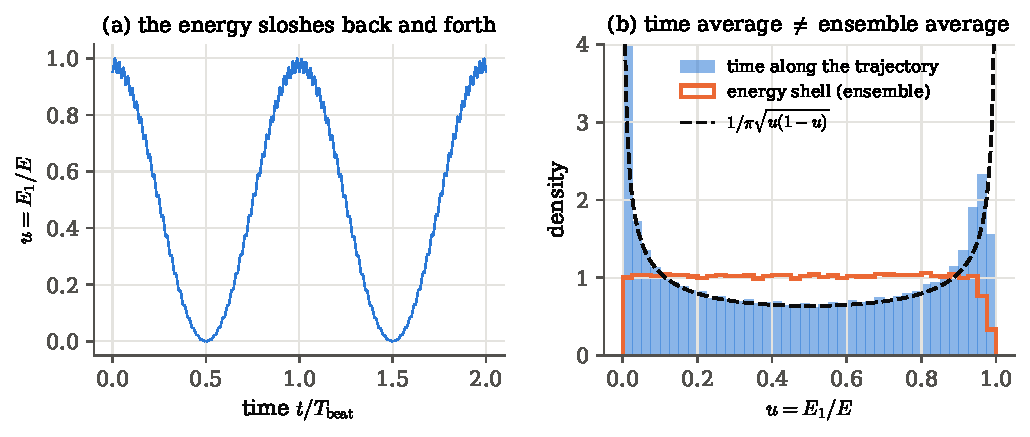
\includegraphics[width=\linewidth]{figures/ch09/two_oscillators.pdf}
\caption{Two weakly coupled oscillators, started with all the energy in the first. (a) The
first oscillator's share of the energy beats between 1 and 0 over two beat periods. (b) The
time the trajectory spends at each share (blue) follows the arcsine curve and crowds at the
ends; the energy shell itself (orange outline) gives every share the same weight. One
trajectory is not a fair sample of the shell.}
\label{9a:fig:two-osc}
\end{figure}

What went wrong is that the motion has more conserved quantities than the energy. Each
normal-mode energy is constant, so the trajectory is trapped on a two-dimensional torus
inside the three-dimensional shell and can never reach the states that the ensemble counts.
Every linear system has this disease, one conserved energy per normal mode, which is why
harmonic crystals do not thermalise on their own and why it took nonlinear couplings,
collisions, or contact with a heat bath to justify statistical mechanics. The lesson is a
sharp version of \cref{ch:01}'s: a motion samples a distribution only if it is ergodic for
that distribution, and that has to be shown, not assumed.

\paragraph{Why this cannot be the general method.}
Even an ergodic motion is rarely usable as a sampler.
\begin{enumerate}[itemsep=1pt]
  \item \emph{Many degrees of freedom.} For $N$ particles the energy shell is a surface of
        dimension $6N-1$. We cannot parametrise it to draw uniform points, and integrating the
        equations of motion for long enough to cover it, if the dynamics covers it at all, is
        as expensive as the problem we started with.
  \item \emph{The canonical ensemble.} A system in contact with a heat bath at temperature
        $T$ is described by $\rho(x,p)\propto e^{-H(x,p)/kT}$. For one oscillator this is a
        product of Gaussians and trivial to sample. For $N$ interacting particles the
        normalisation $\int e^{-H/kT}\dd^{3N}x\,\dd^{3N}p$ has no closed form, there is no
        orbit to follow (the bath changes the energy), and there is no direct sampler.
        Metropolis, the Rosenbluths and the Tellers met exactly this problem for a fluid of
        hard discs, and solved it with a random walk through configurations
        \cite{Metropolis1953}.
  \item \emph{Posteriors have no dynamics.} $p(\params\given\data)\propto\Like(\params)p(\params)$
        is a function on parameter space, known up to $Z$. Nothing moves.
\end{enumerate}
Direct, independent sampling is hard for a second reason too: the generic methods, rejection
sampling and the inverse CDF, need either an envelope that wastes exponentially many draws as
the dimension grows or a CDF we cannot write down \srcref{Lambert}{§12.7}.

So we keep the idea and change the motion. Instead of a deterministic orbit we use a
\emph{random} walker, and we choose its hopping rule so that the fraction of time it spends
anywhere equals the target probability there. The walker will need four properties. Its next
step should depend only on where it is now, so that a step is cheap to compute. The target
should be an equilibrium of its motion. It should forget where it started. And one long walk
should be a fair sample, time averages equal to ensemble averages. The first property defines
a Markov chain; the other three are theorems about Markov chains.

What kind of random walker? The simplest one, which steps left or right with equal chance
wherever it stands, is an \emph{unbiased} walker; it has no preference for any place, so in
the long run it spreads evenly and visits every region equally often
(\cref{9a:sec:diffusion}). That samples only a flat distribution. What we want instead is a
\emph{biased} walker, whose hopping rule depends on the target so that it stays longer where
the target is larger and hurries through where it is small, in exactly the proportion that
makes its fractions of time equal to the target probabilities.
\section{A walker with a memory of one step}
\label{9a:sec:markov}

An elected politician lives on a chain of seven islands, numbered $\theta=1,\dots,7$ from
west to east \srcref{Kruschke}{§7.2.1}. He wants to visit each island in proportion to its
population, but he does not know the total population, nor even how many islands there are.
All his advisers can do is ask the mayor of the island he is on, and the mayor of a
neighbouring island, how many people live there.

\paragraph{Kruschke's question.}
The story is Kruschke's way of asking the question every posterior sampler faces. Can a walker
who never sees a distribution as a whole, only the ratio of its values at two neighbouring
points, still end up visiting every point in proportion to the distribution? For a posterior
the values are $\Like(\params)p(\params)$, which we can compute at any point, and the total is
the evidence $Z$, which we cannot (\cref{9a:sec:roadmap}). If the politician can do without
his total, a sampler can do without $Z$.

\paragraph{His setup.}
Every evening the politician flips a fair coin to propose the island to the east or to the
west. If the proposed island has more people than the current one, he goes. If it has fewer,
he goes only with probability $P_{\rm proposed}/P_{\rm current}$, decided by a spinner marked
from 0 to 1; otherwise he stays another day. Beyond the ends lie two imaginary islands, 0 and
8, where nobody lives, so a proposal to go there is always refused
\srcref{Kruschke}{§7.2.2}. In one table:
\begin{center}
\small
\begin{tabular}{@{}lll@{}}
  \toprule
  ingredient & Kruschke & meaning \\
  \midrule
  islands & $\theta=1,\dots,7$ & the states the walker can be in \\
  populations & $P(\theta)=\theta$ & the target, known only up to its total $28$ \\
  proposal & fair coin: east or west & where to try next, chosen blindly \\
  acceptance & spinner: $\min\bigl(1,P_{\rm proposed}/P_{\rm current}\bigr)$ & the only place the target enters \\
  edges & islands 0 and 8 have $P=0$ & proposals off the ends are refused \\
  \bottomrule
\end{tabular}
\end{center}

\paragraph{The questions.} Suppose he starts on island 4.
\begin{enumerate}[itemsep=1pt]
  \item On day $t$, what is the probability that he is on island $\theta$?
  \item Over a long term of office, what fraction of his days does he spend on each island?
\end{enumerate}
Kruschke's claim is that the second fraction is $\theta/28$, the island's share of the total
population of $1+2+\dots+7=28$, so that the politician reaches his goal without ever learning
the total. His rule is the simplest case of the Metropolis algorithm. To check the claim we
first need to know what kind of object the politician's itinerary is, and how its distribution
moves from day to day; the reason the claim holds is his Eq.~(7.2), which needs only that
description and is derived after the transition matrix.

\subsection{Stochastic processes and the Markov property}
\label{9a:sec:process}

The itinerary $X_1,X_2,X_3,\dots$ is a sequence of random variables, one per day, and the days
are not independent: where he sleeps tomorrow depends on where he slept tonight. A collection
of random variables $\{X_t:t\in\mathcal T\}$ indexed by time is a \newterm{stochastic process}.
The values $X_t$ lie in a set $\mathcal X$, the \newterm{state space}, and $\mathcal T$ is the
\newterm{index set} \mainref{p.~381}. Both may be discrete or continuous.
\begin{itemize}[itemsep=1pt]
  \item An iid sequence $X_1,X_2,\dots$ is a stochastic process, the simplest one, with no
        dependence at all.
  \item The daily weather, $\mathcal X=\{\text{sunny},\text{cloudy}\}$, $\mathcal
        T=\{1,2,\dots\}$: discrete states, discrete time.
  \item A stock price or a detector's baseline voltage recorded continuously: a continuous
        state (for all practical purposes) and continuous time.
  \item The empirical CDF $\widehat F_n(x)=\frac1n\sum_i I(X_i\le x)$ of \cref{ch:03}, viewed
        as a function of $x\in[0,1]$: for each $x$ it is a random variable, so the whole curve
        is a process with continuous state and continuous ``time'' $x$.
\end{itemize}
Any joint distribution can be built up one variable at a time by the product rule of
\cref{ch:01},
\begin{equation}
  f(x_1,\dots,x_n)=f(x_1)\,f(x_2\given x_1)\,f(x_3\given x_1,x_2)\cdots
  f(x_n\given x_1,\dots,x_{n-1})=\prod_{i=1}^n f(x_i\given\text{past}_i),
  \label{9a:eq:product-rule}
\end{equation}
where $\text{past}_i=(x_1,\dots,x_{i-1})$. In general the $i$th factor needs the whole past.
The politician's rule needs much less: his decision tonight uses the population of the island
he is on and of the island he proposes, and nothing about how he got there. The past
influences the future only through the present.

\begin{workdef}[Markov chain]
A discrete-time process $X_0,X_1,X_2,\dots$ with values in a countable state space $\mathcal X$
is a \newterm{Markov chain} if, for every $t$ and every state $x$,
\begin{equation}
  \Prob(X_{t+1}=x\given X_0,X_1,\dots,X_t)=\Prob(X_{t+1}=x\given X_t).
  \label{9a:eq:markov}
\end{equation}
In words: given the present state \unpack{the value of $X_t$, one number}, the next state is
independent of the earlier history \unpack{the values $X_0,\dots,X_{t-1}$}. The chain has a
\newterm{memory of one step}.
\emph{Operational test:} if you can write a simulation whose step $t\to t+1$ reads only the
current state (plus fresh random numbers), the process is a Markov chain.
\end{workdef}

For a Markov chain every conditional in \eqref{9a:eq:product-rule} keeps only its last
argument, and the joint law collapses to a product of one-step factors,
\begin{equation}
  f(x_0,x_1,\dots,x_n)=f(x_0)\,f(x_1\given x_0)\,f(x_2\given x_1)\cdots f(x_n\given x_{n-1}).
  \label{9a:eq:markov-joint}
\end{equation}
As a graph, each variable has a single parent, the one before it
(\cref{9a:fig:dag}a) \mainref{p.~383}. Two remarks place the definition. First, independence is
the special case in which the factor $f(x_{t+1}\given x_t)$ does not depend on $x_t$ at all,
so the Markov property is the mildest generalisation of independence: dependence, but only on
the immediate past \srcref{CasellaBerger}{§5.8.5}. Second, the name records the
\emph{amnesia} of the stepping rule. A chain whose step depends on the last $m$ states is
called a Markov chain of order $m$ \srcref{Lambert}{§12.9}; it becomes an ordinary
(first-order) chain if we take as the state the block of the last $m$ values, so nothing new is
needed for it.

\begin{figure}[htbp]
\centering
\begin{tikzpicture}[
  st/.style={circle,draw=formblue,thick,fill=formblue!8,minimum size=8mm,inner sep=0pt,font=\small},
  ar/.style={->,thick,formblue}]
  \node[font=\small\bfseries] at (-0.6,1.0) {(a)};
  \node[st] (x0) at (0,0) {$X_0$};
  \node[st] (x1) at (1.6,0) {$X_1$};
  \node[st] (x2) at (3.2,0) {$X_2$};
  \node[font=\small] (dots) at (4.6,0) {$\cdots$};
  \node[st] (xn) at (6.0,0) {$X_t$};
  \node[st] (xn1) at (7.6,0) {$X_{t+1}$};
  \draw[ar] (x0) -- (x1); \draw[ar] (x1) -- (x2); \draw[ar] (x2) -- (dots);
  \draw[ar] (dots) -- (xn); \draw[ar] (xn) -- (xn1);
  \begin{scope}[yshift=-2.6cm]
  \node[font=\small\bfseries] at (-0.6,1.1) {(b)};
  \foreach \i in {1,...,7} {
    \node[st,minimum size={(4+0.9*\i)*1mm}] (i\i) at ({(\i-1)*1.27},0) {\i};
  }
  \foreach \i/\j in {1/2,2/3,3/4,4/5,5/6,6/7} {
    \draw[->,thick,tangentgreen] (i\i.north east) to[bend left=35] (i\j.north west);
    \draw[->,thick,bdryred!80!black] (i\j.south west) to[bend left=35] (i\i.south east);
  }
  \node[font=\footnotesize,tangentgreen!70!black,anchor=west] at (8.8,0.55) {east: $\tfrac12$};
  \node[font=\footnotesize,bdryred!80!black,anchor=west] at (8.8,-0.55) {west: $\tfrac12\,\frac{\theta-1}{\theta}$};
  \node[font=\footnotesize,anchor=west] at (8.8,0) {stay: $\frac{1}{2\theta}$};
  \end{scope}
\end{tikzpicture}
\caption{(a) A Markov chain as a graph: each variable depends directly only on the one before
it. (b) The politician's chain. Circles are islands, drawn larger for more populous ones;
upper (green) arrows are moves east, always accepted when proposed, and lower (red) arrows
are moves west, accepted with the population ratio. Island~7's eastward proposal and
island~1's westward one are always refused, which adds to the probability of staying.}
\label{9a:fig:dag}
\end{figure}

\subsection{The transition matrix}
\label{9a:sec:transition}

A Markov chain is \newterm{homogeneous} if the one-step probabilities
$\Prob(X_{t+1}=j\given X_t=i)$ do not change with $t$. All the chains of this chapter are
homogeneous: the politician uses the same rule every night. A homogeneous chain on a finite
state space is then described completely by one square table of numbers.

\begin{workdef}[transition matrix]
For a homogeneous chain on states $1,\dots,K$ the \newterm{transition probabilities} are
$p_{ij}=\Prob(X_{t+1}=j\given X_t=i)$, and the $K\times K$ \newterm{transition matrix} $P$ has
$p_{ij}$ in row $i$ \unpack{the state we are in} and column $j$ \unpack{the state we may move
to}. Every entry is non-negative and every row sums to one,
$\sum_jp_{ij}=1$, because from state $i$ the chain must go somewhere. Each row is a
probability mass function: the forecast for tomorrow given today. A matrix with these two
properties is called a \newterm{stochastic matrix}.
\end{workdef}

\paragraph{Example: Wasserman's weather.}
Suppose sunny and cloudy days follow each other as a Markov chain, the weather tomorrow
depending only on today's \mainref{p.~385}. A typical transition matrix is
\begin{equation}
  P=\begin{pmatrix}0.4&0.6\\0.8&0.2\end{pmatrix}
  \qquad(\text{rows and columns: sunny, cloudy}),
  \label{9a:eq:weather2}
\end{equation}
so after a sunny day there is a 60\% chance of cloud, and after a cloudy day an 80\% chance of
sun. Each row sums to one; the columns need not.

\paragraph{Example: a random walk with absorbing barriers.}
On the states $1,\dots,N$, flip a coin with $\Prob(\text{heads})=p$, $q=1-p$, and step right on
heads and left on tails, except that a walker who reaches $1$ or $N$ stays there forever
\mainref{p.~384}. The transition matrix has $p_{i,i+1}=p$ and $p_{i,i-1}=q$ in the interior
rows and $p_{11}=p_{NN}=1$:
\begin{equation*}
  P=\begin{pmatrix}
     1&0&0&\cdots&0&0\\
     q&0&p&\cdots&0&0\\
     0&q&0&\ddots&0&0\\
     \vdots&&\ddots&\ddots&\ddots&\vdots\\
     0&0&\cdots&q&0&p\\
     0&0&\cdots&0&0&1
  \end{pmatrix}.
\end{equation*}
It is the gambler's ruin: a gambler with $i-1$ units of capital betting one unit at a time
until he is broke or has reached a capital of $N-1$ units.

\paragraph{Example: the politician's matrix.}
From island $\theta$ the politician moves east only if the coin proposes east (probability
$\tfrac12$) and the move is accepted; since $P(\theta+1)>P(\theta)$ it always is. He moves west
only if the coin proposes west and the spinner accepts, which happens with probability
$P(\theta-1)/P(\theta)=(\theta-1)/\theta$. So for an interior island
\begin{align}
  p_{\theta,\theta+1}
  &\eqby{1}\tfrac12\min\Bigl(1,\tfrac{\theta+1}{\theta}\Bigr)=\tfrac12, \nonumber\\
  p_{\theta,\theta-1}
  &\eqby{2}\tfrac12\min\Bigl(1,\tfrac{\theta-1}{\theta}\Bigr)=\frac{\theta-1}{2\theta}, \nonumber\\
  p_{\theta\theta}
  &\eqby{3}1-\tfrac12-\frac{\theta-1}{2\theta}=\frac{1}{2\theta}.
  \label{9a:eq:politician-rows}
\end{align}
\begin{explain}
  \item The probability of a move is (probability of proposing it) $\times$ (probability of
        accepting it); here the proposed island is larger, so acceptance is certain.
  \item The proposed island is smaller, so the spinner accepts with the population ratio.
  \item The rejected proposals keep him where he is, and the row must sum to one.
\end{explain}
At the ends the formulas change only through the empty islands: island 7 never moves east, so
$p_{77}=1-\tfrac{6}{14}=\tfrac47$, and island 1 never moves west, so
$p_{11}=1-\tfrac12=\tfrac12$. Written out,
\begin{equation}
  P=\begin{pmatrix}
   \frac12&\frac12&0&0&0&0&0\\[2pt]
   \frac14&\frac14&\frac12&0&0&0&0\\[2pt]
   0&\frac13&\frac16&\frac12&0&0&0\\[2pt]
   0&0&\frac38&\frac18&\frac12&0&0\\[2pt]
   0&0&0&\frac25&\frac1{10}&\frac12&0\\[2pt]
   0&0&0&0&\frac5{12}&\frac1{12}&\frac12\\[2pt]
   0&0&0&0&0&\frac37&\frac47
  \end{pmatrix}.
  \label{9a:eq:politician-matrix}
\end{equation}
This is the matrix Kruschke builds symbolically in his Eq.~(7.3) \srcref{Kruschke}{§7.2.5}.
The script builds it in four lines, which are the rule itself:
\pyfile[firstline=22,lastline=28,firstnumber=22]{code/ch09/03_island_hopping.py}{The politician's transition matrix, built from the proposal and the acceptance rule}
Line 27 is ``propose with probability $\tfrac12$, accept with $\min(1,\text{ratio})$''; line 26
skips the empty islands, whose proposals are never accepted; line 28 puts every refused
proposal on the diagonal.

\paragraph{His key equation, in our symbols.}
Kruschke's notation and ours name the same things differently. His island $\theta$ is our
state $i$; his relative population $P(\theta)$ is our target $\pi_i$, up to the factor $28$;
his ``probability of moving from $\theta$ to $\theta+1$'' is our matrix entry
$p_{\theta,\theta+1}$. His Eq.~(7.2) compares the two directions across one bridge between
neighbouring islands. Dividing the first line of \eqref{9a:eq:politician-rows} by the second
line written for island $\theta+1$,
\begin{equation*}
  \frac{p_{\theta,\theta+1}}{p_{\theta+1,\theta}}
  =\frac{\tfrac12}{\tfrac12\,\theta/(\theta+1)}
  =\frac{P(\theta+1)}{P(\theta)} :
\end{equation*}
the ratio of the two hopping probabilities equals the ratio of the two populations, and the
total $28$ never appears. Why this ratio forces the long-run fractions to be $\theta/28$ is the
subject of detailed balance (\cref{9a:sec:detailed-balance}), where the same equation is
rearranged into a statement about traffic across each bridge.

\subsection{How a distribution moves: $p_{t+1}=p_tP$}
\label{9a:sec:evolve}

We now answer the first question. Write the probabilities of being in each state on day $t$ as
a \emph{row} vector $p_t=(p_t(1),\dots,p_t(K))$, with $p_t(j)=\Prob(X_t=j)$. Today's
distribution and the transition matrix fix tomorrow's: to be in $j$ tomorrow the walker must be
somewhere today and then jump to $j$, and the possible ``somewheres'' are disjoint, so
\begin{align}
  p_{t+1}(j)
  &\eqby{1}\sum_{i}\Prob(X_t=i,\;X_{t+1}=j)
  \eqby{2}\sum_i\Prob(X_t=i)\,\Prob(X_{t+1}=j\given X_t=i) \nonumber\\
  &\eqby{3}\sum_i p_t(i)\,p_{ij},
  \qquad\text{i.e.}\qquad p_{t+1}=p_t\,P .
  \label{9a:eq:evolve}
\end{align}
\begin{explain}
  \item Law of total probability over today's state $i$ (\cref{ch:01}).
  \item Product rule.
  \item Definitions of $p_t$ and of $p_{ij}$; homogeneity lets us drop the $t$ from $p_{ij}$.
        The sum over $i$ of a row vector times the $i$th row of $P$ is the vector--matrix
        product.
\end{explain}
One step of the chain is one multiplication by $P$ from the right. A stochastic matrix maps
probability vectors to probability vectors: the entries of $p_tP$ are sums of non-negative
terms, and they add up to $\sum_j\sum_ip_t(i)p_{ij}=\sum_ip_t(i)\sum_jp_{ij}=1$.

\begin{pitfall}[Rows or columns?]
Probabilists write distributions as row vectors and multiply by $P$ on the right, so the
\emph{rows} of $P$ sum to one. Much of the physics literature (master equations, quantum
channels) writes column vectors and uses the transpose. Before using a formula from elsewhere,
check which index is ``from'' and which is ``to''. The stationary distribution is a \emph{left}
eigenvector of $P$ in our convention.
\end{pitfall}

\paragraph{Example: the politician's first two nights.}
On day 1 he is on island 4 for sure, $p_1=(0,0,0,1,0,0,0)$. Multiplying a vector with a single
1 in position 4 by $P$ picks out row 4 of \eqref{9a:eq:politician-matrix}:
\begin{equation*}
  p_2=p_1P=\bigl(0,\,0,\,\tfrac38,\,\tfrac18,\,\tfrac12,\,0,\,0\bigr)
       =(0,0,\NineAIslTwoThree,\NineAIslTwoFour,\NineAIslTwoFive,0,0),
\end{equation*}
the three bars of Kruschke's panel $t=2$ \srcref{Kruschke}{§7.2.3}. On day 3,
\begin{align*}
  p_3(2)&\eqby{1}\tfrac38\cdot\tfrac13=\tfrac18, &
  p_3(3)&\eqby{2}\tfrac38\cdot\tfrac16+\tfrac18\cdot\tfrac38=\tfrac{7}{64}, &
  p_3(4)&\eqby{3}\tfrac38\cdot\tfrac12+\tfrac18\cdot\tfrac18+\tfrac12\cdot\tfrac25=\tfrac{129}{320},\\
  p_3(5)&\eqby{4}\tfrac18\cdot\tfrac12+\tfrac12\cdot\tfrac1{10}=\tfrac{9}{80}, &
  p_3(6)&\eqby{5}\tfrac12\cdot\tfrac12=\tfrac14, &
  p_3(1)&=p_3(7)=0 .
\end{align*}
\begin{explain}
  \item Island 2 can be reached on day 3 only from island 3 (moving west, probability
        $p_{32}=\frac13$).
  \item From island 3 by staying ($p_{33}=\frac16$) or from island 4 by moving west
        ($p_{43}=\frac38$).
  \item From 3 eastwards, from 4 by staying, from 5 westwards ($p_{54}=\frac25$).
  \item From 4 eastwards and from 5 by staying ($p_{55}=\frac1{10}$).
  \item From 5 eastwards.
\end{explain}
These are $\NineAIslThreeTwo,\ \NineAIslThreeThree,\ \NineAIslThreeFour,\
\NineAIslThreeFive,\ \NineAIslThreeSix$, and they add up to one. After two nights he can be
at most two islands from where he started, so islands 1 and 7 still have probability zero.

\paragraph{What $p_t$ means, and how to simulate a chain.}
$p_t$ is not what one politician does; one politician is on exactly one island each day. It is
the histogram of where a large number of independent politicians would be on day $t$, all
following the same rule from the same starting distribution \mainref{p.~386}. Simulating one
of them needs only the initial distribution $p_0$ and $P$: draw $X_0$ from $p_0$; if it came
out $i$, draw $X_1$ from row $i$ of $P$; if that came out $j$, draw $X_2$ from row $j$; and so
on. In code, each draw from a row is one uniform number compared with the row's cumulative
sums (the inverse-CDF method of \cref{ch:06}); that is all \pyname{walk} and
\pyname{step_many} in \texttt{lib\_markov.py} do.

\paragraph{What we compute.}
Two things, for the same days Kruschke drew. The exact crowd histogram comes from repeated
multiplication, $p_t=p_1P^{t-1}$, with $P$ the matrix \eqref{9a:eq:politician-matrix} and $p_1$
the spike on island 4. The simulated one comes from running $\NineAIslWalkers$ independent
politicians from island 4 and counting where they sleep on day $t$. The two are drawn together
in \cref{9a:fig:island-dist} for days 2, 3, 5, 13 and 99. The early distributions are
lopsided, with a bulge over the starting island; by day 13 the shape is already close to a
straight incline.

\paragraph{Side by side with Kruschke.}
Kruschke's Fig.~7.3 shows the same sequence of histograms as bars, read off his matrix
\srcref{Kruschke}{§7.2.3}. At $t=2$ there is something exact to compare; at later days the
natural comparison is with the incline $\theta/28$ itself, measured by the total-variation
distance $\tfrac12\sum_\theta\abs{p_t(\theta)-\theta/28}$ (the largest difference in
probability that any set of islands can show, defined in \cref{9a:sec:convergence}).
\begin{center}
\small
\begin{tabular}{@{}lll@{}}
  \toprule
  quantity & Kruschke, Fig.~7.3 & ours \\
  \midrule
  $p_2(3),\,p_2(4),\,p_2(5)$ & $0.375,\ 0.125,\ 0.5$ & $\NineAIslTwoThree,\ \NineAIslTwoFour,\ \NineAIslTwoFive$ \\
  day 13, distance from $\theta/28$ & close to the incline (by eye) & $\NineAIslTVThirteen$ \\
  day 99, distance from $\theta/28$ & indistinguishable (by eye) & $\NineAIslTVNinetyNine$ \\
  \bottomrule
\end{tabular}
\end{center}
The day-2 values agree exactly, as they must: both are row 4 of the same matrix. What the
calculation adds is the size of the remaining difference on later days, a number instead of a
picture; how fast it shrinks is the subject of \cref{9a:sec:convergence}.

\begin{figure}[htbp]
\centering
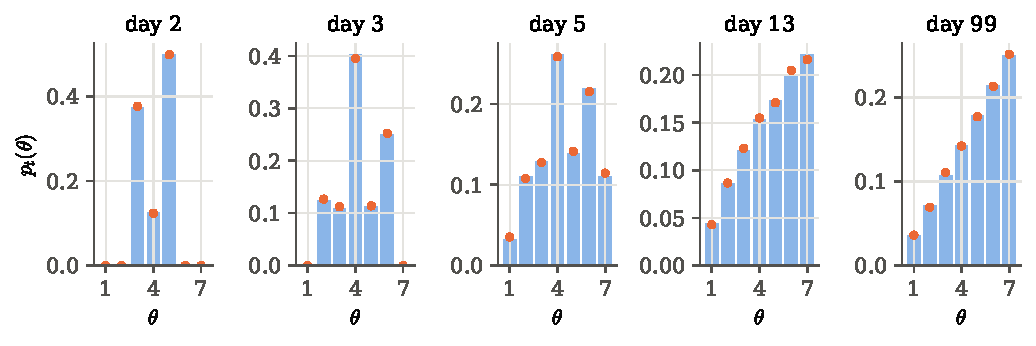
\includegraphics[width=\linewidth]{figures/ch09/island_distributions.pdf}
\caption{Where the politician is likely to be, starting from island 4. Bars are the exact
$p_t=p_1P^{t-1}$; dots are the fractions of $2\times10^4$ simulated politicians. The
distribution spreads from its starting spike, overshoots, and settles into the incline
$p(\theta)=\theta/28$, the same for every later day.}
\label{9a:fig:island-dist}
\end{figure}

\paragraph{Many steps at once: the Chapman--Kolmogorov equations.}
Let $p_{ij}(n)=\Prob(X_{m+n}=j\given X_m=i)$ be the probability of going from $i$ to $j$ in
exactly $n$ steps, and $P_n$ the matrix of these \newterm{$n$-step transition probabilities}
\mainref{p.~385}. To go from $i$ to $j$ in $m+n$ steps the chain must be somewhere, say $k$,
after the first $m$ of them:
\begin{align}
  p_{ij}(m+n)
  &= \Prob(X_{m+n}=j\given X_0=i)
  \eqby{1}\sum_k\Prob(X_{m+n}=j,\;X_m=k\given X_0=i) \nonumber\\
  &\eqby{2}\sum_k\Prob(X_{m+n}=j\given X_m=k,\;X_0=i)\,\Prob(X_m=k\given X_0=i) \nonumber\\
  &\eqby{3}\sum_k\Prob(X_{m+n}=j\given X_m=k)\,\Prob(X_m=k\given X_0=i)
  \eqby{4}\sum_k p_{ik}(m)\,p_{kj}(n).
  \label{9a:eq:chapman}
\end{align}
\begin{explain}
  \item Law of total probability over the intermediate state, inside the conditional
        probability given $X_0=i$.
  \item Product rule in its conditional form,
        $\Prob(A,B\given C)=\Prob(B\given C)\Prob(A\given B,C)$.
  \item The Markov property: once $X_m=k$ is known, $X_0$ is irrelevant for the future. (For
        $n>1$ this uses \eqref{9a:eq:markov} repeatedly, one step at a time.)
  \item Homogeneity: the probabilities depend only on the number of steps.
\end{explain}
The last line is matrix multiplication, so $P_{m+n}=P_mP_n$. Since $P_1=P$, we get
$P_2=P^2$, $P_3=P^3$ and in general
\begin{equation}
  P_n=P^n,\qquad p_n=p_0P^n .
  \label{9a:eq:pn}
\end{equation}
The second statement follows from the first by one more use of total probability,
$p_n(j)=\sum_i\Prob(X_n=j\given X_0=i)\Prob(X_0=i)=\sum_ip_0(i)\,p_{ij}(n)$, or simply by
applying \eqref{9a:eq:evolve} $n$ times. Every question about a homogeneous finite chain is
therefore a question about the powers of one matrix, and the long-run behaviour is the
behaviour of $P^n$ as $n\to\infty$, which is a question about eigenvalues.

\paragraph{Example: the weather a week ahead.}
For Wasserman's weather \eqref{9a:eq:weather2}, starting on a sunny day, $p_0=(1,0)$:
$p_1=(0.4,0.6)$, $p_2=(0.4\cdot0.4+0.6\cdot0.8,\;\dots)=(0.64,0.36)$,
$p_3=(\NineAWTwoSunThree,\ \dots)$, and $p_6(\text{sunny})=\NineAWTwoSunSix$. The forecast
swings above and below a value near $0.571$ with a shrinking amplitude. \Cref{9a:sec:convergence}
shows that the value is $4/7$ and that the swing shrinks by the factor $-0.4$ each day.

\subsection{The long run, seen in one trajectory}
\label{9a:sec:onetrip}

The second question is about a single politician over a long time, not about a crowd on one
day. \Cref{9a:fig:island-traj}a shows the first 500 days of one simulated trip on a logarithmic
time axis, like Kruschke's Fig.~7.2: the politician wanders down to island 1 early on, then
drifts east and spends most of his time among the larger islands. Counting his days over a trip
of $\NineAIslDays$ days (\cref{9a:fig:island-traj}b), the fraction spent on each island differs
from $\theta/28$ by at most $\NineAIslMaxDev$. The time he spends on an island tracks its
population.

\paragraph{Two different facts.}
\Cref{9a:fig:island-dist,9a:fig:island-traj} look alike but answer different questions. The
first is a histogram over many politicians on one day $t$: it approaches $\theta/28$ as $t$
grows, which is convergence of $p_t$ (\cref{9a:sec:convergence}). The second is a histogram
over the days of one politician: it approaches $\theta/28$ as the trip grows, which is the
ergodic theorem (\cref{9a:sec:ergodic}). Neither implies the other on sight: a crowd can
settle while each member keeps a lopsided personal history, and one long history can be fair
even when the crowd never settles (\cref{9a:sec:not-convergent}). Kruschke stops at showing that
$\theta/28$ is \emph{stable}, leaving the rest as ``far beyond'' his book
\srcref{Kruschke}{§7.2.5}; both facts are proved in \cref{9a:sec:convergence,9a:sec:ergodic}.

\paragraph{The lesson.} Reproducing the island figures turns a picture that ``looks settled''
into two separate limits, one over walkers and one over time, and only the second is what a
single MCMC run relies on.

\begin{figure}[htbp]
\centering
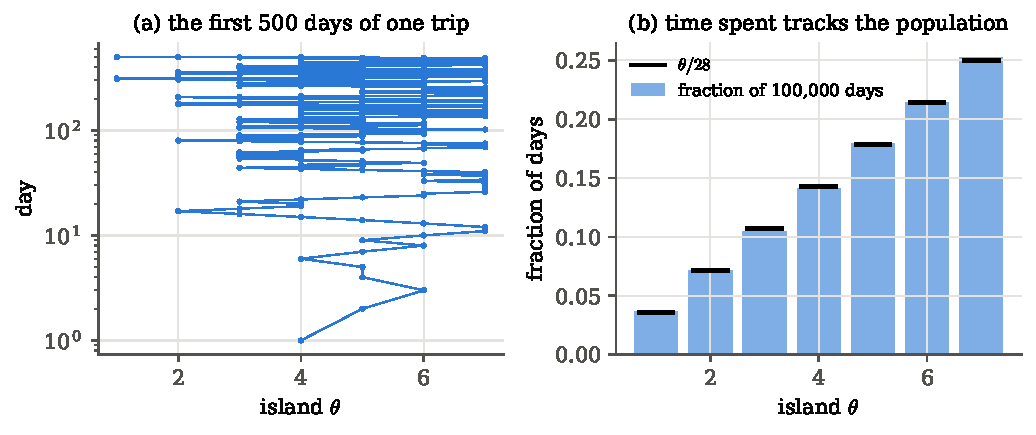
\includegraphics[width=\linewidth]{figures/ch09/island_trajectory.pdf}
\caption{(a) One politician's first 500 days, with the day on a logarithmic axis so that the
early wandering is visible. (b) The fraction of $10^5$ days he spends on each island (bars)
against the population shares $\theta/28$ (black ticks).}
\label{9a:fig:island-traj}
\end{figure}

\subsection{Reading the transition matrix off a history}
\label{9a:sec:mle}

So far $P$ was given and we predicted the walk. The inverse question also arises: we observe
one history $x_0,x_1,\dots,x_n$ of a chain (a weather record, a sequence of detector states)
and want to infer $P$. By \eqref{9a:eq:markov-joint} the probability of the observed history is
a product of one-step factors, one per observed transition. Collecting equal factors, with
$n_{ij}$ the number of observed transitions from $i$ to $j$,
\begin{equation}
  \Like(p_0,P)=p_0(x_0)\prod_{r=1}^{n}p_{x_{r-1}x_r}=p_0(x_0)\prod_{i,j}p_{ij}^{\,n_{ij}}
  \label{9a:eq:chain-like}
\end{equation}
\mainref{p.~394}. There is only one observation of the starting state, so $p_0$ cannot be
learned; we maximise over $P$. Take the logarithm of \eqref{9a:eq:chain-like},
\begin{equation*}
  \ln\Like=\ln p_0(x_0)+\sum_i\Bigl(\sum_jn_{ij}\ln p_{ij}\Bigr).
\end{equation*}
The first term does not contain $P$ at all, so it plays no part in the maximisation. The rest is
a sum of one bracket per row $i$, and each bracket contains only the entries of its own row.
The constraints are also one per row, $\sum_jp_{ij}=1$. So changing row $i$ changes only its
own bracket, and each row can be maximised on its own, with its own Lagrange multiplier
$\mu_i$ (the method of \cref{ch:03} for maximising under a constraint):
\begin{align}
  0&\eqby{1}\frac{\partial}{\partial p_{ij}}\Bigl[\sum_kn_{ik}\ln p_{ik}-\mu_i\Bigl(\sum_kp_{ik}-1\Bigr)\Bigr]
   =\frac{n_{ij}}{p_{ij}}-\mu_i
   \quad\Longrightarrow\quad p_{ij}=\frac{n_{ij}}{\mu_i}, \nonumber\\
  1&\eqby{2}\sum_jp_{ij}=\frac{n_i}{\mu_i}
   \quad\Longrightarrow\quad
   \hat p_{ij}=\frac{n_{ij}}{n_i},\qquad n_i=\sum_jn_{ij}.
  \label{9a:eq:chain-mle}
\end{align}
\begin{explain}
  \item The part of $\ln\Like$ that involves row $i$, plus the constraint for that row; set
        the derivative to zero. Only the $k=j$ terms depend on $p_{ij}$, and
        $\partial(n_{ij}\ln p_{ij})/\partial p_{ij}=n_{ij}/p_{ij}$, so the condition is
        $n_{ij}/p_{ij}=\mu_i$, that is $p_{ij}=n_{ij}/\mu_i$. It is a maximum: the second
        derivative of each term, $-n_{ij}/p_{ij}^2$, is negative, so the bracket is concave in
        the row and its only stationary point on the constraint is the top.
  \item Impose the constraint to find $\mu_i$: it equals $n_i$, the number of departures from
        state $i$.
\end{explain}
The estimate is the obvious one: of the $n_i$ times we left state $i$, the fraction that went
to $j$.

\emph{How uncertain is it?} Fix a row $i$ and look only at the $n_i$ nights the chain spent
in state $i$. By the Markov property each departure from $i$ is a fresh draw from row $i$ of $P$,
whatever happened before, so the $n_i$ destinations are independent draws from the same pmf
$(p_{i1},\dots,p_{iK})$. Counting how many went to each $j$ is then exactly the multinomial
setting of \cref{2a:sec:multinomial}, with $n_i$ trials and cell probabilities $p_{ij}$:
\begin{equation*}
  \Var(n_{ij})=n_ip_{ij}(1-p_{ij}),\qquad \Cov(n_{ij},n_{i\ell})=-n_ip_{ij}p_{i\ell}\quad(j\ne\ell).
\end{equation*}
Dividing the counts by $n_i$ gives the estimate $\hat p_{ij}=n_{ij}/n_i$, whose variance is
$p_{ij}(1-p_{ij})/n_i$, so its error bar is $\sqrt{\hat p_{ij}(1-\hat p_{ij})/n_i}$. Different
rows use different nights, so their errors are uncorrelated. For large $n_i$ the multinomial
counts are close to Normal (the central limit theorem applied to the sum of $n_i$ indicator
vectors), which gives $\sqrt{n_i}(\hat p_{ij}-p_{ij})\rightsquigarrow\Normal$ with variance
$p_{ij}(1-p_{ij})$ \mainref{p.~394, Thm~23.31}.

One thing differs from ordinary multinomial counting: $n_i$ is not fixed in advance but is
itself random, since it depends on how often the chain happened to visit $i$. For an ergodic
chain the fraction of time spent in $i$ settles to $\pi_i$ (\cref{9a:sec:ergodic}), so $n_i$
grows like $n\pi_i$ as the record lengthens, every row gets more and more departures, and the
estimate is consistent with the error bar above shrinking as $1/\sqrt{n\pi_i}$.

\paragraph{Example: a thousand days of weather.}
The script \texttt{08\_markov\_mle.py} simulates $\NineAMLEn$ days of the three-state weather
chain used throughout \cref{9a:sec:convergence} (sunny, cloudy, rainy; true rainy row
$(0.6,0,0.4)$). The record visits sun, cloud and rain $\NineAMLEnS$, $\NineAMLEnC$ and
$\NineAMLEnR$ times, and gives for the rainy row
$\hat p_{RS}=\NineAMLERS\pm\NineAMLEseRS$ and $\hat p_{RR}=\NineAMLERR\pm\NineAMLEseRR$, the error
bars being $\sqrt{\hat p(1-\hat p)/n_R}$. Rain is the rarest state, so its row is the least
well measured. Repeating the experiment on $\NineAMLERep$ independent histories, the
standardised error $(\hat p_{RS}-p_{RS})/\sqrt{p_{RS}(1-p_{RS})/n_R}$ has mean
$\NineAMLEzMean$ and standard deviation $\NineAMLEzSd$, and its histogram is a standard
Normal (\cref{9a:fig:mle}): the multinomial error bar is right even though the visits to
rain arrive in correlated clumps.

\begin{figure}[htbp]
\centering
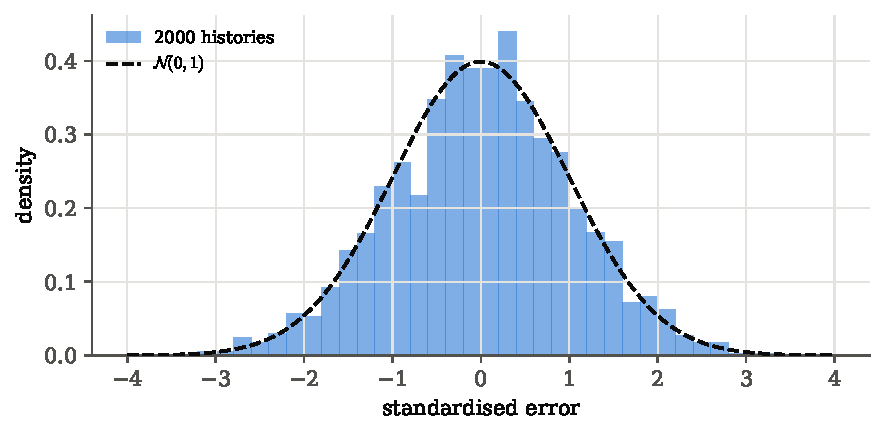
\includegraphics[width=0.75\linewidth]{figures/ch09/markov_mle.pdf}
\caption{The error of the estimated rain-to-sun probability, in units of its multinomial
standard error, over $2000$ simulated thousand-day records. The histogram follows the
standard Normal curve.}
\label{9a:fig:mle}
\end{figure}
\section{Who can reach whom: classifying the states}
\label{9a:sec:classify}

Not every Markov chain settles down. A fish that swims into a net never visits the rest of
the ocean again; a rollercoaster car runs round its track forever and is at the top of the
loop only at regular instants \srcref{Lambert}{§13.6.2}. Both are perfectly good Markov
chains, but neither has a long-run histogram that is independent of where it started: the
fish's histogram depends on when it was caught, and the car's distribution at time $t$ keeps
rotating instead of settling. Wasserman's Fig.~23.2 shows the same contrast for two simulated
chains, one wandering off for good, one fluctuating about a fixed level \mainref{p.~384}. Before
proving that a chain converges we need words for the ways in which it can fail to: some
states cannot be reached from others, some states are left and never revisited, and some are
revisited only in a fixed rhythm.

\paragraph{The questions.} For a given transition matrix $P$:
\begin{enumerate}[itemsep=1pt]
  \item From state $i$, can the chain ever get to state $j$?
  \item Having left $i$, is it certain to come back, and how long does that take on average?
  \item Can it come back at any time, or only at multiples of some period?
\end{enumerate}

\subsection{Communication and irreducibility}
\label{9a:sec:communicate}

State $i$ \newterm{reaches} $j$ (or $j$ is \newterm{accessible} from $i$), written $i\to j$,
if $p_{ij}(n)>0$ for some $n\ge0$; we count $n=0$, so every state reaches itself. If $i\to j$
and $j\to i$ the two states \newterm{communicate}, $i\leftrightarrow j$ \mainref{p.~387}.

Communication is an equivalence relation: it is reflexive ($n=0$), symmetric by definition,
and transitive, because if $i\to j$ in $m$ steps and $j\to k$ in $n$ steps then
\begin{align*}
  p_{ik}(m+n)
  &\eqby{1}\sum_\ell p_{i\ell}(m)\,p_{\ell k}(n)
  \relby{2}{\ge} p_{ij}(m)\,p_{jk}(n)
  \relby{3}{>}0 .
\end{align*}
\begin{explain}
  \item Chapman--Kolmogorov \eqref{9a:eq:chapman}.
  \item All terms are non-negative; keep only the term $\ell=j$.
  \item Both factors are positive by assumption.
\end{explain}
An equivalence relation cuts the state space into disjoint \newterm{communicating classes},
$\mathcal X=\mathcal X_1\cup\mathcal X_2\cup\cdots$, with two states in the same class exactly
when they communicate \mainref{p.~387, Thm~23.12}.

\begin{workdef}[irreducible, closed, absorbing]
A chain is \newterm{irreducible} if all its states communicate \unpack{one single class, every
state reachable from every other in some number of steps}. A set of states is
\newterm{closed} if the chain can never leave it once inside \unpack{$p_{ij}=0$ for every $i$
in the set and $j$ outside it}. A closed set consisting of one state is an
\newterm{absorbing state} \unpack{$p_{ii}=1$}.
\emph{Operational test:} draw the transition graph, an arrow $i\to j$ for every nonzero
$p_{ij}$. The chain is irreducible if and only if from every node there is a path of arrows to
every other node.
\end{workdef}

\paragraph{Example: four states, three classes.}
Wasserman's Ex.~23.13 has $\mathcal X=\{1,2,3,4\}$ and
\begin{equation*}
  P=\begin{pmatrix}
    \tfrac13&\tfrac23&0&0\\[1pt]
    \tfrac23&\tfrac13&0&0\\[1pt]
    \tfrac14&\tfrac14&\tfrac14&\tfrac14\\[1pt]
    0&0&0&1
  \end{pmatrix}.
\end{equation*}
Reading the graph (\cref{9a:fig:classes}a): 1 and 2 send arrows only to each other, so
$\{1,2\}$ is a class, and it is closed. State 3 sends arrows everywhere, but nothing comes back
to 3 from any other state, so $\{3\}$ is a class on its own, and not closed. State 4 has
$p_{44}=1$: $\{4\}$ is a closed class and 4 is absorbing. A walker that starts in 3 stays
there for a geometric number of steps (mean $1/(1-\tfrac14)=\tfrac43$) and then falls for good
into $\{1,2\}$ or into $4$. The odds of the two exits follow from row 3. Each night in state 3
the walker leaves with probability $1-\tfrac14=\tfrac34$; it goes to 1 or 2 with probability
$\tfrac14+\tfrac14=\tfrac12$ and to 4 with probability $\tfrac14$. Given that it leaves, the
chances are therefore $(\tfrac12)/(\tfrac34)=\tfrac23$ for $\{1,2\}$ and
$(\tfrac14)/(\tfrac34)=\tfrac13$ for $4$, the same on every night, so these are also the
chances of the eventual exit. Where it ends up depends on luck, so this chain has no unique
long-run histogram.

The politician's chain \eqref{9a:eq:politician-matrix} is irreducible: every island sends an
arrow to each neighbour, so any island reaches any other by a walk along the chain. The
absorbing random walk of \cref{9a:sec:transition} is not: its classes are $\{1\}$, $\{N\}$
(both absorbing) and the interior $\{2,\dots,N-1\}$, which is not closed.

\begin{figure}[htbp]
\centering
\begin{tikzpicture}[
  st/.style={circle,draw=formblue,thick,fill=formblue!8,minimum size=7mm,inner sep=0pt,font=\small},
  ar/.style={->,thick,formblue},
  cl/.style={draw=tangentgreen!70!black,dashed,rounded corners=4pt,thick}]
  \node[font=\small\bfseries] at (-0.9,1.4) {(a)};
  \node[st] (a1) at (0,0.8) {1};
  \node[st] (a2) at (0,-0.8) {2};
  \node[st] (a3) at (1.9,0) {3};
  \node[st] (a4) at (3.6,0) {4};
  \draw[ar] (a1) to[bend left=25] (a2);
  \draw[ar] (a2) to[bend left=25] (a1);
  \draw[ar] (a3) -- (a1); \draw[ar] (a3) -- (a2); \draw[ar] (a3) -- (a4);
  \draw[ar] (a1) to[loop above,looseness=6] (a1);
  \draw[ar] (a2) to[loop below,looseness=6] (a2);
  \draw[ar] (a3) to[loop above,looseness=6] (a3);
  \draw[ar] (a4) to[loop above,looseness=6] (a4);
  \draw[cl] (-0.6,-2.05) rectangle (0.6,2.05);
  \draw[cl] (3.1,-0.55) rectangle (4.1,1.25);
  \node[font=\footnotesize,tangentgreen!60!black] at (0,-2.35) {closed};
  \node[font=\footnotesize,tangentgreen!60!black] at (3.6,-0.85) {absorbing};
  \node[font=\footnotesize,bdryred!80!black] at (1.9,-0.85) {transient};
  \node[font=\small\bfseries] at (5.1,1.4) {(b)};
  \node[st] (b1) at (6.4,0.9) {1};
  \node[st] (b2) at (7.4,-0.8) {2};
  \node[st] (b3) at (5.4,-0.8) {3};
  \draw[ar] (b1) -- (b2); \draw[ar] (b2) -- (b3); \draw[ar] (b3) -- (b1);
  \node[font=\footnotesize] at (6.4,-1.6) {period 3};
  \node[font=\small\bfseries] at (8.6,1.4) {(c)};
  \node[st] (c1) at (9.2,0.8) {1};
  \node[st] (c2) at (9.2,-0.8) {2};
  \node[st] (c3) at (10.7,0.8) {3};
  \node[st] (c4) at (10.7,-0.8) {4};
  \node[st] (c5) at (12.2,0.8) {5};
  \node[st] (c6) at (12.2,-0.8) {6};
  \draw[ar] (c1) to[bend left=20] (c2); \draw[ar] (c2) to[bend left=20] (c1);
  \draw[ar] (c5) to[bend left=20] (c6); \draw[ar] (c6) to[bend left=20] (c5);
  \draw[ar] (c3) -- (c1); \draw[ar] (c3) -- (c2); \draw[ar] (c3) to[bend left=20] (c4);
  \draw[ar] (c4) to[bend left=20] (c3); \draw[ar] (c4) -- (c1); \draw[ar] (c4) -- (c6);
  \draw[cl] (8.75,-1.3) rectangle (9.65,1.3);
  \draw[cl] (11.75,-1.3) rectangle (12.65,1.3);
  \node[font=\footnotesize,bdryred!80!black] at (10.7,-1.6) {transient};
\end{tikzpicture}
\caption{Transition graphs, an arrow for every nonzero transition probability. (a) Wasserman's
Ex.~23.13: $\{1,2\}$ is a closed class, 4 is absorbing, and 3 leaks into both and is never
re-entered. (b) A deterministic cycle: the chain returns to each state only every third
step. (c) Ex.~23.28 (self-loops not drawn): two closed classes $\{1,2\}$ and $\{5,6\}$, and
states 3 and 4 that eventually drain into one of them.}
\label{9a:fig:classes}
\end{figure}

\subsection{Coming back: recurrence and transience}
\label{9a:sec:recurrence}

Start the chain in state $i$. Will it ever come back? State $i$ is \newterm{recurrent} (or
persistent) if
\begin{equation*}
  \Prob(X_n=i\text{ for some }n\ge1\given X_0=i)=1,
\end{equation*}
and \newterm{transient} otherwise \mainref{p.~388}. The test is the expected number of visits.

\begin{keyidea}[Recurrence $\Leftrightarrow$ infinitely many expected returns]
State $i$ is recurrent if and only if $\sum_{n}p_{ii}(n)=\infty$, and transient if and only
if $\sum_np_{ii}(n)<\infty$ \mainref{p.~388, Thm~23.15}.
\end{keyidea}

\paragraph{Why.}
Let $I_n=1$ if $X_n=i$ and $0$ otherwise, so that $Y=\sum_{n\ge0}I_n$ counts the visits to $i$.
Its mean, for a chain started at $i$, is
\begin{align}
  \E(Y\given X_0=i)
  &\eqby{1}\sum_{n=0}^\infty\E(I_n\given X_0=i)
   \eqby{2}\sum_{n=0}^\infty\Prob(X_n=i\given X_0=i)
   \eqby{3}\sum_{n=0}^\infty p_{ii}(n) .
  \label{9a:eq:visits}
\end{align}
\begin{explain}
  \item Linearity of expectation, which holds for infinite sums of non-negative terms.
  \item The mean of an indicator is the probability of its event.
  \item Definition of the $n$-step probability.
\end{explain}
Now count the visits differently. Let $a_i$ be the probability of ever returning. Each time
the chain is at $i$, the Markov property makes the future a fresh copy of the chain started at
$i$, so it returns again with probability $a_i$, independently of the past. If $a_i=1$ it
returns, returns again, and so on forever: $Y=\infty$ with probability one, and
\eqref{9a:eq:visits} diverges. If $a_i<1$, each visit is the last with probability $1-a_i$, so
$Y$ is geometric:
\begin{align*}
  \Prob(Y=k\given X_0=i)=a_i^{k-1}(1-a_i),\qquad
  \E(Y\given X_0=i)
  &\eqby{1}\sum_{k\ge1}k\,a_i^{k-1}(1-a_i)
   \eqby{2}\frac{1-a_i}{(1-a_i)^2}=\frac{1}{1-a_i}<\infty .
\end{align*}
\begin{explain}
  \item Mean of the geometric distribution with ``success'' (no return) probability $1-a_i$.
  \item $\sum_kka^{k-1}=\frac{\dd}{\dd a}\sum_ka^k=1/(1-a)^2$ for $\abs a<1$.
\end{explain}
So a finite sum means transience and an infinite one means recurrence. For a finite chain
there is a shortcut for the general facts \mainref{p.~389, Thm~23.16}: recurrence and
transience are properties of a whole class (if $i$ is recurrent and $i\leftrightarrow j$, then
$j$ is recurrent, and likewise for transient); a finite chain has at least one recurrent state
(it runs forever on finitely many states, so some state is visited infinitely often); and in a
finite irreducible chain every state is recurrent. The state space always splits as
$\mathcal X=\mathcal X_T\cup\mathcal X_1\cup\mathcal X_2\cup\cdots$, the transient states
$\mathcal X_T$ plus closed irreducible classes of recurrent states (the \newterm{decomposition
theorem}, \mainref{p.~389, Thm~23.17}). In \cref{9a:fig:classes}a, $\mathcal X_T=\{3\}$ and the
closed classes are $\{1,2\}$ and $\{4\}$.

\paragraph{Example: the random walk on the integers.}
A walker on $\{\dots,-1,0,1,\dots\}$ steps $+1$ with probability $p$ and $-1$ with $q=1-p$
\mainref{p.~389, Ex.~23.18}. All states communicate, so either all are recurrent or all are
transient; test state 0. A return can happen only after an even number of steps, $2n$, with
exactly $n$ steps each way, in any order, so $p_{00}(2n)=\binom{2n}{n}p^nq^n$. Stirling's
formula $n!\simeq n^n e^{-n}\sqrt{2\pi n}$ gives the size of the binomial coefficient:
\begin{align}
  \binom{2n}{n}=\frac{(2n)!}{(n!)^2}
  &\eqby{1}\frac{(2n)^{2n}e^{-2n}\sqrt{4\pi n}}{n^{2n}e^{-2n}\,2\pi n}
   \eqby{2}\frac{4^n}{\sqrt{\pi n}},
  \qquad\text{so}\qquad
  p_{00}(2n)\simeq\frac{(4pq)^n}{\sqrt{\pi n}} .
  \label{9a:eq:stirling-walk}
\end{align}
\begin{explain}
  \item Stirling for $(2n)!$ in the numerator and for each $n!$ in the denominator.
  \item $(2n)^{2n}/n^{2n}=4^n$ and $\sqrt{4\pi n}/(2\pi n)=1/\sqrt{\pi n}$.
\end{explain}
Since $pq\le\tfrac14$ with equality only at $p=\tfrac12$, two cases appear. For $p\ne\tfrac12$,
$4pq<1$ and the terms decrease geometrically, the sum converges, and the walk is transient: it
drifts away in the direction of the bias and returns only finitely often. For $p=\tfrac12$,
$p_{00}(2n)\simeq1/\sqrt{\pi n}$, whose sum diverges like $\sqrt n$, and the walk is
recurrent. Stirling is already good at $n=10$, where exact over approximate is
$\NineARetStirTen$ (\cref{9a:fig:return}a).

The two cases can also be checked against the geometric law of the visits. The expected number
of visits to 0, counting the start, is the full sum \eqref{9a:eq:visits}, and the binomial
series $\sum_{n\ge0}\binom{2n}{n}x^n=(1-4x)^{-1/2}$ (valid for $\abs{x}<\tfrac14$) sums it in
closed form with $x=pq$:
\begin{align*}
  \sum_{n\ge0}p_{00}(2n)
  &\eqby{1}(1-4pq)^{-1/2}
   \eqby{2}\bigl((p-q)^2\bigr)^{-1/2}
   \eqby{3}\frac{1}{\abs{p-q}}.
\end{align*}
\begin{explain}
  \item The binomial series with $x=pq$.
  \item $1-4pq=(p+q)^2-4pq=p^2-2pq+q^2=(p-q)^2$, using $p+q=1$.
  \item The positive square root of a square is the absolute value.
\end{explain}
The same mean is $1/(1-a)$ by the geometric law of the visits found above, so
$1/(1-a)=1/\abs{p-q}$, and the probability of ever returning is $a=1-\abs{p-q}$.
For $p=0.6$: $x=0.24$, $(1-0.96)^{-1/2}=0.04^{-1/2}=5$ visits on average including the start,
so $\sum_{n\ge1}p_{00}(2n)=\NineARetSumSix$ after removing the $n=0$ term, and the probability of
ever returning is $a=1-\tfrac15=0.8=1-\abs{0.6-0.4}$. Simulating $\NineARetWalkers$ walkers for
$\NineARetSteps$ steps (\cref{9a:fig:return}b), the fraction that has come back at least once is
$\NineARetSix$ for $p=0.6$, and $\NineARetHalf$ for $p=\tfrac12$, still creeping towards one.

\emph{How fast the symmetric walker comes home.} For $p=\tfrac12$ there is an exact
statement: the probability of no return by step $2n$ equals the probability $p_{00}(2n)$ of
being at the origin at step $2n$. A quick check at $n=1$: the walker fails to return at step 2
with probability $\tfrac12$, and $p_{00}(2)=\binom21\tfrac14=\tfrac12$. The general proof uses
the series above once more. Write $u_n=p_{00}(2n)$ and $f_n$ for the probability that the
\emph{first} return happens at step $2n$. Being at 0 at step $2n\ge2$ means a first return at
some step $2k\le2n$ followed, by the Markov property, by being back at 0 after $2n-2k$ more steps,
so $u_n=\sum_{k=1}^nf_ku_{n-k}$. Multiply by $s^n$ and sum over $n$; with
$U(s)=\sum_{n\ge0}u_ns^n$ and $F(s)=\sum_{n\ge1}f_ns^n$ this reads $U=1+FU$, and the binomial
series with $x=s/4$ gives $U(s)=(1-s)^{-1/2}$. Then
\begin{align*}
  \sum_{n\ge0}\Prob(T_{00}>2n)\,s^n
  &\eqby{1}\sum_{n\ge0}\Bigl(1-\sum_{k=1}^{n}f_k\Bigr)s^n
   \eqby{2}\frac{1-F(s)}{1-s}
   \eqby{3}\frac{1}{(1-s)\,U(s)}
   \eqby{4}(1-s)^{-1/2}=U(s).
\end{align*}
\begin{explain}
  \item No return by step $2n$ means the first return comes later than step $2n$.
  \item $\sum_ns^n=1/(1-s)$, and $\sum_n s^n\sum_{k\le n}f_k=F(s)/(1-s)$ (each $f_k$ appears
        in every term with $n\ge k$).
  \item $U=1+FU$ gives $1-F=1/U$.
  \item $U(s)=(1-s)^{-1/2}$.
\end{explain}
Two power series that are equal have equal coefficients, so
$\Prob(T_{00}>2n)=p_{00}(2n)\simeq1/\sqrt{\pi n}$ by \eqref{9a:eq:stirling-walk}, which
predicts the returned fraction $\NineARetHalfPred$ seen in the simulation.

\begin{figure}[htbp]
\centering
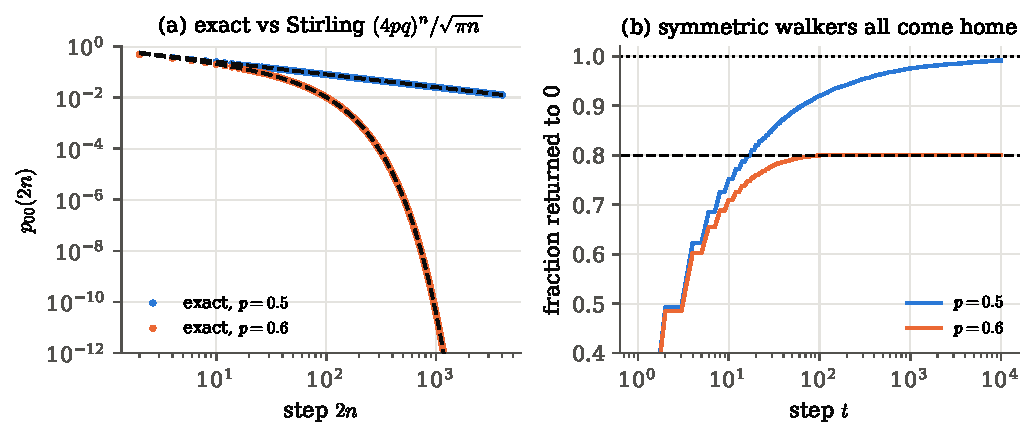
\includegraphics[width=\linewidth]{figures/ch09/return_probability.pdf}
\caption{(a) The probability of being back at the origin after $2n$ steps: exact (dots) and
Stirling's approximation (dashed). The symmetric walk decays only as $1/\sqrt n$; a bias of
$0.6$ makes it decay geometrically. (b) The fraction of $10^4$ walkers that have returned to
the origin at least once: all of them eventually for the symmetric walk, $80\%$ for the biased
one (dashed line).}
\label{9a:fig:return}
\end{figure}

\paragraph{How long until it comes back?}
Recurrence says that the return happens; it does not say how soon. The \newterm{recurrence
time} $T_{ii}=\min\{n>0:X_n=i\}$ (for $X_0=i$) has distribution
$f_{ii}(n)=\Prob(X_1\ne i,\dots,X_{n-1}\ne i,X_n=i\given X_0=i)$ and the \newterm{mean
recurrence time} is $m_i=\E(T_{ii})=\sum_nnf_{ii}(n)$ \mainref{p.~390}. A recurrent state with
$m_i=\infty$ is \newterm{null recurrent}; otherwise it is \newterm{positive recurrent}.

\emph{A mean from the tail.} For a waiting time $T$ taking values $1,2,3,\dots$ there is a
convenient way to compute the mean. Write $T$ as a count of the steps $k=0,1,\dots,T-1$ before
it, $T=\sum_{k\ge0}I(T>k)$, with $I$ the indicator ($1$ if true, $0$ if not),, and take expectations term by term (all terms are
non-negative):
\begin{equation*}
  \E(T)=\sum_{k\ge0}\Prob(T>k).
\end{equation*}
The mean is finite exactly when the tail probabilities $\Prob(T>k)$ have a finite sum.

\emph{The symmetric walk is null.} The symmetric walk on the integers is the standard
null-recurrent chain: every walker comes home, but the probability of not yet being home after
$2n$ steps is $p_{00}(2n)\simeq1/\sqrt{\pi n}$, as just shown. Each value $\Prob(T_{00}>2n)$
appears twice in the tail sum (for $k=2n$ and $k=2n+1$, since returns happen only at even
steps), so $\E(T_{00})\approx\sum_n2/\sqrt{\pi n}$, which diverges like $\sqrt n$. At a
null-recurrent state the walker is certain to return, yet the chance of finding it at home at
any given late time goes to zero, $p_{ii}(n)\to0$, because it spends longer and longer
excursions away \mainref{p.~390, Lemma~23.19}; the symmetric walk shows it directly, with
$p_{00}(2n)\simeq1/\sqrt{\pi n}$. We will meet the null walker again as the free diffusion of
\cref{9a:sec:diffusion}.

\emph{A finite chain has no null states.} Take a state $i$ in a closed irreducible class of a
finite chain. From every state $j$ of the class some path leads to $i$, and we may take it of
length at most $M$, the number of states (a shortest path never visits a state twice). Its
probability is positive, and since there are only finitely many $j$, the smallest of these
probabilities is some $\varepsilon>0$. So wherever the walker stands, the chance of reaching $i$
within the next $M$ steps is at least $\varepsilon$, and by the Markov property this holds
afresh for each block of $M$ steps. Missing $i$ in $k$ blocks in a row therefore has probability
at most $(1-\varepsilon)^k$:
\begin{equation*}
  \Prob(T_{ii}>kM)\le(1-\varepsilon)^k,
  \qquad
  m_i=\sum_{n\ge0}\Prob(T_{ii}>n)\le M\sum_{k\ge0}(1-\varepsilon)^k=\frac{M}{\varepsilon}<\infty,
\end{equation*}
using the tail formula and the fact that $\Prob(T_{ii}>n)$ can only decrease with $n$, so each
block of $M$ terms is at most $M$ times its first term. A geometric tail leaves no room for the
ever-longer excursions of a null state: in a finite chain every recurrent state is positive
recurrent \mainref{p.~390, Lemma~23.20}.

\subsection{Rhythm: periodicity}
\label{9a:sec:period}

The deterministic cycle $1\to2\to3\to1$ (\cref{9a:fig:classes}b),
\begin{equation*}
  P=\begin{pmatrix}0&1&0\\0&0&1\\1&0&0\end{pmatrix},
\end{equation*}
started in state 1 is in state 1 at times $0,3,6,9,\dots$ and never in between
\mainref{p.~390}. The \newterm{period} of state $i$ is
$d(i)=\gcd\{n\ge1:p_{ii}(n)>0\}$, the greatest common divisor of the possible return times; $i$
is \newterm{periodic} if $d(i)>1$ and \newterm{aperiodic} if $d(i)=1$. Period is a class
property: communicating states have the same period (Lemma~23.21). Two quick tests cover most
chains met in practice. A single self-loop ($p_{ii}>0$) makes the period 1, since then $1$ is a
possible return time. A walk that alternates between two sets, such as $\pm1$ steps on a ring of
even length, has period 2: it returns only after an even number of steps. The politician's
chain is aperiodic because every island has $p_{\theta\theta}=1/(2\theta)>0$; refused
proposals act as self-loops. A ``tilted'' die that always moves to a neighbouring face round the
ring of six faces \srcref{Lambert}{§12.10} has period 2, and we will see in
\cref{9a:sec:ergodic} what that does and does not spoil.

\paragraph{Example: four lakes on a ring.}
Lambert's marooned fisherman camps each evening beside one of four lakes $A,B,C,D$ joined in a
ring \srcref{Lambert}{§13.3}. He wants to fish each lake in proportion to its fish stock, so he uses
the politician's rule: flip a coin to propose the clockwise or the anticlockwise neighbour, go
there if it holds more fish, and otherwise go with probability equal to the ratio of the stocks.
If the four stocks were equal, every proposal would be accepted and he would alternate between
$\{A,C\}$ and $\{B,D\}$: period 2. Take stocks in the ratio $1:2:4:3$ (our numbers). Then
\begin{equation*}
  P=\begin{pmatrix}
    0&\tfrac12&0&\tfrac12\\[1pt]
    \tfrac14&\tfrac14&\tfrac12&0\\[1pt]
    0&\tfrac14&\tfrac38&\tfrac38\\[1pt]
    \tfrac16&0&\tfrac12&\tfrac13
  \end{pmatrix}
\end{equation*}
(rows and columns $A,B,C,D$; for example $p_{CD}=\tfrac12\cdot\tfrac34$ and $p_{CC}=1-\tfrac14-\tfrac38$).
Lake $A$ has no self-loop, since both neighbours are bigger and every proposal is accepted, but
$B$, $C$ and $D$ have refused proposals, hence $p_{ii}>0$ and period 1. Communicating states
share their period, so the whole chain is aperiodic: unequal stocks break the rhythm that
equal stocks would impose. The chain is also irreducible, so it is ergodic, and
$\pi=(0.1,0.2,0.4,0.3)$ balances every pair of neighbours (for instance
$\pi_Ap_{AB}=0.05=\pi_Bp_{BA}$).

\begin{workdef}[ergodic state and chain]
A state is \newterm{ergodic} if it is recurrent, non-null \unpack{finite mean return time}
and aperiodic \unpack{return times have greatest common divisor 1}. A chain is ergodic if all
its states are \mainref{p.~390, Def.~23.22}.
\emph{Operational test for a finite chain:} it is ergodic if and only if it is irreducible and
aperiodic, and then some power $P^m$ has every entry strictly positive.
\end{workdef}

\paragraph{Why some power of $P$ is strictly positive.}
The operational test in the box rests on a small fact about numbers. Fix a state $i$ and let
$R_i=\{n\ge1:p_{ii}(n)>0\}$ be its possible return times.

\emph{Return times can be added.} If $m$ and $n$ are in $R_i$, so is $m+n$: by
Chapman--Kolmogorov \eqref{9a:eq:chapman}, $p_{ii}(m+n)=\sum_kp_{ik}(m)p_{ki}(n)\ge
p_{ii}(m)\,p_{ii}(n)>0$, keeping only the term $k=i$ (go round one loop, then the other).

\emph{Coprime loops fill in every large number.} Aperiodic means $\gcd(R_i)=1$. Take the simplest
case, return times $3$ and $5$. Adding them in all combinations gives $3a+5b$ for whole numbers
$a,b\ge0$, and these include $8=3+5$, $9=3\cdot3$, $10=5\cdot2$, and then every larger number,
because adding $3$ to $8,9,10$ gives $11,12,13$, and so on. Only $1,2,4,7$ are missed. The
same holds for any set of positive integers with greatest common divisor 1 that is closed under
addition (a classical fact of elementary number theory, of which the $3,5$ case is the
pattern): it contains every integer beyond some $N_i$. So the walker can return to $i$ in
\emph{exactly} $n$ steps for every $n\ge N_i$.

\emph{Then go anywhere.} For any pair $i,j$, irreducibility gives a path from $i$ to $j$ of some
length $\ell_{ij}$ with $p_{ij}(\ell_{ij})>0$. Waste $N_i+k$ steps looping at $i$, then take
the path:
\begin{equation*}
  p_{ij}(N_i+k+\ell_{ij})\ge p_{ii}(N_i+k)\,p_{ij}(\ell_{ij})>0\qquad\text{for every }k\ge0 .
\end{equation*}

\emph{One power for all pairs.} There are finitely many pairs, so take $m$ larger than every
$N_i+\ell_{ij}$. Then $p_{ij}(m)>0$ for all $i,j$, which is $P^m>0$ entrywise. Finally, a
finite irreducible chain is automatically positive recurrent (\cref{9a:sec:recurrence}, the
geometric-tail argument), so irreducible and aperiodic is all the test needs.

\paragraph{Example: six states.}
Wasserman's Ex.~23.28 has
\begin{equation*}
  P=\begin{pmatrix}
    \tfrac12&\tfrac12&0&0&0&0\\[1pt]
    \tfrac14&\tfrac34&0&0&0&0\\[1pt]
    \tfrac14&\tfrac14&\tfrac14&\tfrac14&0&0\\[1pt]
    \tfrac14&0&\tfrac14&\tfrac14&0&\tfrac14\\[1pt]
    0&0&0&0&\tfrac12&\tfrac12\\[1pt]
    0&0&0&0&\tfrac12&\tfrac12
  \end{pmatrix}
\end{equation*}
\mainref{p.~392}. Rows 1--2 and 5--6 send probability only within $\{1,2\}$ and $\{5,6\}$, so
these are closed irreducible classes. States 3 and 4 communicate with each other, but the path
$3\to4\to6$ leads into $\{5,6\}$, from which there is no way back, so 3 and 4 are transient.
Every state has a self-loop, so all are aperiodic: 1, 2, 5 and 6 are ergodic, 3 and 4 are
transient (\cref{9a:fig:classes}c). The chain as a whole is not irreducible, and its long-run
behaviour depends on which closed class swallows the walker.

\paragraph{Irreducible is not the same as ergodic.}
Some texts say ``irreducible (or ergodic)'' \srcref{Lambert}{§13.6.2}, but these are different
conditions. The deterministic 3-cycle is irreducible but periodic, so its distribution at time
$t$ never settles; the symmetric random walk on the integers is irreducible and recurrent but
null, so it has no equilibrium at all. Irreducibility says the chain can get everywhere;
ergodicity adds that it comes back often enough and without a fixed rhythm. The vocabulary of
classification, collected:
\begin{center}
\small
\begin{tabularx}{\linewidth}{@{}lXl@{}}
\toprule
property & meaning & example \\
\midrule
transient & left for good with positive probability & state 3 of \cref{9a:fig:classes}a\\
null recurrent & returns surely, mean return time infinite & symmetric walk on $\Z$\\
positive recurrent & returns, finite mean return time & any state of a finite irreducible chain\\
periodic ($d>1$) & returns only at multiples of $d$ & deterministic 3-cycle\\
ergodic & positive recurrent and aperiodic & every island of the politician\\
\bottomrule
\end{tabularx}
\end{center}
\section{Equilibrium: stationary distributions and detailed balance}
\label{9a:sec:stationary}

Go back to the crowd of independent politicians of \cref{9a:sec:evolve}, all following the
island-hopping rule. Suppose that tonight the crowd happens to be spread over the islands in
proportion to their populations, a fraction $\theta/28$ on island $\theta$. Tomorrow some of
them move east, some west, some stay. Kruschke's ``climactic implication'' is that the crowd is
still spread as $\theta/28$ \srcref{Kruschke}{§7.2.5}: individuals move, the histogram does
not. This is what equilibrium means for a random walk, and it is the property that makes the
target distribution something a chain can settle into.

\paragraph{The question.} Is there a distribution of the walkers that one step of the chain
leaves unchanged? If so, is there only one, and how do we find it without solving for it?

\begin{workdef}[stationary distribution]
A probability vector $\pi=(\pi_1,\dots,\pi_K)$ \unpack{non-negative entries that sum to one}
is a \newterm{stationary} (or invariant) distribution of the chain if
\begin{equation}
  \pi=\pi P,\qquad\text{that is}\qquad \pi_j=\sum_i\pi_i\,p_{ij}\quad\text{for every }j .
  \label{9a:eq:stationary}
\end{equation}
It is a left eigenvector of $P$ with eigenvalue 1 \mainref{p.~390, Def.~23.23}.
\emph{Operational recipe:} solve the linear system $\pi(P-\Id)=0$ together with
$\sum_i\pi_i=1$, or compute the left eigenvector of $P$ for eigenvalue 1 and normalise it
(\pyname{stationary} in \texttt{lib\_markov.py}).
\end{workdef}

If the chain starts in a stationary distribution it stays there forever. With $X_0\sim\pi$,
\eqref{9a:eq:pn} gives $p_1=\pi P=\pi$, $p_2=\pi P^2=(\pi P)P=\pi P=\pi$, and by induction
$p_n=\pi P^n=\pi$ for all $n$ \mainref{p.~391}. Each individual walker keeps moving; only the
distribution of the crowd is frozen.

A stationary vector always exists for a finite chain, because the eigenvalue 1 always occurs:
the rows of $P$ sum to one, which says $P\mathbf1=\mathbf1$ for the column vector $\mathbf1$ of
ones, so 1 is an eigenvalue of $P$, and a matrix and its transpose have the same eigenvalues,
so there is also a left eigenvector. That this left eigenvector can be chosen with non-negative
entries, and that it is unique when the chain is irreducible, are the content of the
Perron--Frobenius theorem; \cref{9a:sec:convergence} proves both by a direct argument.

\paragraph{Balance of flows.}
Think of probability as a conserved fluid on the states, with $\pi_ip_{ij}$ the amount that
flows from $i$ to $j$ in one step. Write the stationarity condition \eqref{9a:eq:stationary} for
state $j$ in two ways, separating in each the part that stays put at $j$:
\begin{align*}
  \pi_j&\eqby{1}\sum_i\pi_i\,p_{ij}=\pi_j\,p_{jj}+\sum_{i\ne j}\pi_i\,p_{ij},\\
  \pi_j&\eqby{2}\pi_j\sum_k p_{jk}=\pi_j\,p_{jj}+\sum_{k\ne j}\pi_j\,p_{jk}.
\end{align*}
\begin{explain}
  \item Stationarity: what is at $j$ tomorrow is what arrives from everywhere, including from
        $j$ itself; take the $i=j$ term out of the sum.
  \item Row $j$ of $P$ sums to one, so multiplying $\pi_j$ by that sum changes nothing; take
        the $k=j$ term out.
\end{explain}
The left sides are equal, so the right sides are. Cancel the common term $\pi_jp_{jj}$, the
probability that sits at $j$ and stays:
\begin{equation}
  \underbrace{\sum_{i\ne j}\pi_i\,p_{ij}}_{\text{flow into }j}
  \;=\;
  \underbrace{\sum_{k\ne j}\pi_j\,p_{jk}}_{\text{flow out of }j}
  \qquad\text{for every }j .
  \label{9a:eq:global-balance}
\end{equation}
Stationarity is \newterm{global balance}: at every state the inflow equals the outflow, like
Kirchhoff's current law at every node of a circuit. It does not say that the flow along each
wire vanishes. That stronger statement is detailed balance, below.

\paragraph{Example: Wasserman's weather.}
For \eqref{9a:eq:weather2} the first component of $\pi=\pi P$ reads
$\pi_S=0.4\pi_S+0.8\pi_C$, so $0.6\pi_S=0.8\pi_C$, and with $\pi_S+\pi_C=1$,
$\pi=(\tfrac47,\tfrac37)$. In the long run four days in seven are sunny. For a general two-state
chain with $a=p_{12}$ and $b=p_{21}$ the same two lines give
\begin{equation}
  \pi=\Bigl(\frac{b}{a+b},\ \frac{a}{a+b}\Bigr),
  \label{9a:eq:pi-two}
\end{equation}
the flow balance $\pi_1a=\pi_2b$ in disguise: the state that is harder to leave gets more
weight.

\paragraph{Example: a three-state weather chain.}
Our running example of a chain has states sunny (S), cloudy (C) and rainy (R) and
\begin{equation}
  P=\begin{pmatrix}0.6&0.2&0.2\\0.3&0.7&0\\0.6&0&0.4\end{pmatrix}.
  \label{9a:eq:weather3}
\end{equation}
Cloud tends to persist; rain clears straight to sun, and there is no direct cloud--rain
transition in either direction. The three equations of $\pi=\pi P$ are
\begin{align*}
  \pi_S&=0.6\pi_S+0.3\pi_C+0.6\pi_R,&
  \pi_C&=0.2\pi_S+0.7\pi_C,&
  \pi_R&=0.2\pi_S+0.4\pi_R .
\end{align*}
The second gives $\pi_C=\tfrac23\pi_S$, the third $\pi_R=\tfrac13\pi_S$ (the first is then
automatic, since the three equations add up to an identity), and normalisation gives
\begin{equation}
  \pi=\bigl(\tfrac12,\ \tfrac13,\ \tfrac16\bigr).
  \label{9a:eq:pi-weather3}
\end{equation}

\paragraph{Example: the Hardy--Weinberg law.}
A gene comes in two types $A$ and $a$, and each person carries two copies, so people are of
genotype $AA$, $Aa$ or $aa$ \mainref{p.~392, Ex.~23.29}. Each parent passes on one of its two
copies at random, and mates are chosen at random.

\emph{The gene pool.} Let a population have genotype fractions $r$ ($AA$), $s$ ($Aa$) and
$1-r-s$ ($aa$). Pool all the genes: an $AA$ person contributes two $A$'s, an $Aa$ person one
$A$ out of two, so the fraction of $A$ genes in the pool is $g=r+s/2$, and the fraction of $a$
genes is $h=1-g$. A child gets one gene from each parent, each an independent draw from the
pool, so it is $AA$ with probability $g^2$, $Aa$ with $2gh$ (an $A$ from either parent) and
$aa$ with $h^2$. Its own genes then carry the fraction $g^2+\tfrac12(2gh)=g(g+h)=g$ of $A$: the
gene frequency does not change, and from the second generation on the genotype fractions are
$(g^2,2gh,h^2)$, the Hardy--Weinberg law.

\emph{One family line.} Now follow a single person and their descendants, one child per
generation, each child's other parent drawn at random from the population. The genotype of the
$n$th descendant depends only on the genotype of the $(n-1)$th (and on the fixed pool), so it is
a Markov chain on $\{AA,Aa,aa\}$. Its rows come from asking what each parent passes on.
\begin{itemize}[itemsep=1pt]
  \item An $AA$ parent always passes $A$; the mate passes $A$ with probability $g$. The child is
        $AA$ with probability $g$ and $Aa$ with $h$.
  \item An $Aa$ parent passes $A$ or $a$ with probability $\tfrac12$ each. The child is $AA$ if
        both pass $A$, probability $\tfrac12g$; $aa$ if both pass $a$, probability $\tfrac12h$;
        and $Aa$ otherwise, probability $\tfrac12h+\tfrac12g=\tfrac12$ (using $g+h=1$).
  \item An $aa$ parent always passes $a$. The child is $Aa$ with probability $g$ and $aa$ with $h$.
\end{itemize}
So
\begin{equation*}
  P=\begin{pmatrix} g&h&0\\ \tfrac g2&\tfrac12&\tfrac h2\\ 0&g&h\end{pmatrix}.
\end{equation*}
\emph{Hardy--Weinberg is stationary.} Take $\pi=(g^2,2gh,h^2)$ and check $\pi P=\pi$ component
by component, using $g+h=1$,
\begin{align*}
  (\pi P)_{AA}&=g^2\cdot g+2gh\cdot\tfrac g2=g^2(g+h)=g^2,\\
  (\pi P)_{Aa}&=g^2\cdot h+2gh\cdot\tfrac12+h^2\cdot g=gh(g+h)+gh=2gh,\\
  (\pi P)_{aa}&=2gh\cdot\tfrac h2+h^2\cdot h=h^2(g+h)=h^2 .
\end{align*}
\emph{From the crowd to one line.} The chain is irreducible when $0<g<1$ (every genotype can
reach every other within two generations) and aperiodic (the diagonal entries are positive), so
by the ergodic theorem (\cref{9a:sec:ergodic}) the fraction of its generations that one family
line spends as $AA$ tends to $\pi_{AA}=g^2$: the same as the fraction of $AA$ people in any one
generation.

\subsection{Stationary does not mean convergent}
\label{9a:sec:not-convergent}

A stationary distribution is an equilibrium. Whether the chain ever reaches it is a different
question \mainref{p.~392, Ex.~23.27}. The deterministic 3-cycle of \cref{9a:sec:period} has
the uniform distribution $\pi=(\tfrac13,\tfrac13,\tfrac13)$ as a stationary distribution
($\pi P$ just permutes the three equal entries). Started in $\pi$ it stays in $\pi$. Started in
state 1 it is in state 1, then 2, then 3, then 1 again: $p_t$ is a spike that rotates forever,
and its distance from $\pi$ never shrinks (\cref{9a:fig:cycles}, blue). What does converge is the
\emph{time average} of $p_t$ over a period, which is uniform; we will see in
\cref{9a:sec:ergodic} that time averages need less than distributions do.

The chain has a \newterm{limiting distribution} $\pi$ if the rows of $P^n$ all converge to the
same vector $\pi$,
\begin{equation}
  \lim_{n\to\infty}p_{ij}(n)=\pi_j\quad\text{for every }i,
  \qquad\text{i.e.}\qquad
  P^n\to\begin{pmatrix}\pi\\ \pi\\ \vdots\\ \pi\end{pmatrix}
  \label{9a:eq:limiting}
\end{equation}
\mainref{p.~391, Def.~23.24}. Then $p_n=p_0P^n\to\sum_ip_0(i)\pi=\pi$ for every initial
distribution: the chain forgets where it started. The 3-cycle has a stationary distribution but
no limiting one.

\subsection{Detailed balance}
\label{9a:sec:detailed-balance}

Kruschke's argument for why the island rule works starts not from $\pi=\pi P$ but from pairs
of neighbouring islands \srcref{Kruschke}{§7.2.5, Eq.~(7.2)}. The ratio of the probability of
hopping east from $\theta$ to that of hopping back west from $\theta+1$ is, by
\eqref{9a:eq:politician-rows},
\begin{equation*}
  \frac{p_{\theta,\theta+1}}{p_{\theta+1,\theta}}
  =\frac{\tfrac12}{\tfrac12\,\theta/(\theta+1)}
  =\frac{\theta+1}{\theta}
  =\frac{P(\theta+1)}{P(\theta)} .
\end{equation*}
Rearranged, $P(\theta)\,p_{\theta,\theta+1}=P(\theta+1)\,p_{\theta+1,\theta}$: with the crowd
spread in proportion to the populations, as many politicians cross from $\theta$ to $\theta+1$
each night as cross back. Every bridge carries equal traffic both ways.

\begin{workdef}[detailed balance]
A distribution $\pi$ satisfies \newterm{detailed balance} with respect to $P$ if
\begin{equation}
  \pi_i\,p_{ij}=\pi_j\,p_{ji}\qquad\text{for every pair }i,j
  \label{9a:eq:detailed-balance}
\end{equation}
\unpack{the probability flow from $i$ to $j$ equals the flow from $j$ to $i$, for each pair
separately} \mainref{p.~391, (23.15)}. A chain with such a $\pi$ is called
\newterm{reversible}.
\emph{Operational test:} for each pair with $p_{ij}>0$, check that $p_{ji}>0$ and that
$p_{ij}/p_{ji}=\pi_j/\pi_i$. Only ratios of $\pi$ enter.
\end{workdef}

Detailed balance is stronger than stationarity, and it implies it. Sum
\eqref{9a:eq:detailed-balance} over $i$:
\begin{align}
  (\pi P)_j=\sum_i\pi_i\,p_{ij}
  &\eqby{1}\sum_i\pi_j\,p_{ji}
   \eqby{2}\pi_j\sum_ip_{ji}
   \eqby{3}\pi_j .
  \label{9a:eq:db-implies}
\end{align}
\begin{explain}
  \item Detailed balance, term by term.
  \item $\pi_j$ does not depend on the summation index.
  \item Row $j$ of $P$ sums to one.
\end{explain}
That is the whole proof \mainref{p.~391, Thm~23.26}. Compare it with Kruschke's verification of
stationarity for the islands, which needs the four cases of whether each neighbour is larger
or smaller \srcref{Kruschke}{§7.2.5, Eq.~(7.4)}: detailed balance does all four at once.

\begin{keyidea}[Detailed balance $\Rightarrow$ stationary]
If $\pi_ip_{ij}=\pi_jp_{ji}$ for all pairs, then $\pi P=\pi$. To build a chain with a
prescribed stationary distribution it is enough to make every pair of moves balance, and that
needs only the ratios $\pi_j/\pi_i$, never the normalisation of $\pi$.
\end{keyidea}

\paragraph{Example: the politician's equilibrium.}
For the islands, \eqref{9a:eq:detailed-balance} holds with $\pi_\theta\propto\theta$ for each
pair of neighbours (just shown), and trivially for non-neighbours, where both sides are zero.
So $\pi_\theta=\theta/28$ is stationary. The politician never needed the total population 28:
his rule uses only the ratio of two neighbouring populations, and the ratio is all detailed
balance asks for. That is the whole secret of the Metropolis algorithm, and why it can sample a
posterior whose evidence $Z$ is unknown \cite{Metropolis1953,Hastings1970}.

\paragraph{Example: the three-state weather chain is reversible.}
For \eqref{9a:eq:weather3} with $\pi=(\tfrac12,\tfrac13,\tfrac16)$:
$\pi_Sp_{SC}=\tfrac12\cdot0.2=0.1=\tfrac13\cdot0.3=\pi_Cp_{CS}$;
$\pi_Sp_{SR}=\tfrac12\cdot0.2=0.1=\tfrac16\cdot0.6=\pi_Rp_{RS}$; and
$\pi_Cp_{CR}=0=\pi_Rp_{RC}$. Each of the three ``bridges'' carries $0.1$ of the probability each
way per day (\cref{9a:fig:currents}a).

\paragraph{The physical picture: equilibrium without currents.}
In statistical mechanics, detailed balance is the statement that in thermal equilibrium every
elementary process is balanced by its reverse: as many molecules react $A\to B$ per second as
react $B\to A$, as many photons are absorbed in a transition as are emitted in the reverse one.
This principle of microscopic reversibility is what made Einstein's $A$ and $B$ coefficients
consistent with the Planck spectrum. There are no net probability currents anywhere. A
stationary state can exist with currents, however, as a steady current flows round a circuit
driven by a battery: global balance \eqref{9a:eq:global-balance} holds at every node, but the
flow on each wire does not vanish. Such states are \emph{non-equilibrium steady states}.

\paragraph{Example: a biased cycle has a stationary distribution but no detailed balance.}
On a ring of three states let the walker step clockwise with probability $0.6$, anticlockwise
with $0.2$, and stay with $0.2$:
\begin{equation*}
  P=\begin{pmatrix}0.2&0.6&0.2\\0.2&0.2&0.6\\0.6&0.2&0.2\end{pmatrix}.
\end{equation*}
Its columns sum to one as well as its rows (a \newterm{doubly stochastic} matrix), so the
uniform $\pi=(\tfrac13,\tfrac13,\tfrac13)$ is stationary: $(\pi P)_j=\tfrac13\sum_ip_{ij}=\tfrac13$.
But $\pi_1p_{12}=0.2\ne\pi_2p_{21}=0.0\overline{6}$. Each edge carries a net clockwise current
$J=\tfrac13(0.6-0.2)=\NineACycJ$ per step, the same on all three edges, so the inflow and
outflow balance at every node while probability circulates for ever (\cref{9a:fig:currents}b).
A reversible chain could not do this. Going round any closed loop of states, detailed balance
forces the product of the transition probabilities one way to equal the product the other way,
because the $\pi$'s cancel ($p_{12}p_{23}p_{31}=\frac{\pi_2}{\pi_1}p_{21}\cdot\frac{\pi_3}{\pi_2}p_{32}
\cdot\frac{\pi_1}{\pi_3}p_{13}$), and here $0.6^3\ne0.2^3$. (The converse also holds, and this
loop test is Kolmogorov's criterion for reversibility.)

\begin{figure}[htbp]
\centering
\begin{tikzpicture}[
  st/.style={circle,draw=formblue,thick,fill=formblue!8,minimum size=9mm,inner sep=0pt,font=\small},
  fw/.style={->,thick,tangentgreen!70!black},
  bw/.style={->,thick,bdryred!80!black}]
  \node[font=\small\bfseries] at (-1.6,1.9) {(a)};
  \node[st] (S) at (0,1.2) {S};
  \node[st] (C) at (-1.3,-0.9) {C};
  \node[st] (R) at (1.3,-0.9) {R};
  \draw[fw] (S) to[bend right=18] (C);
  \draw[bw] (C) to[bend right=18] (S);
  \draw[fw] (S) to[bend left=18] (R);
  \draw[bw] (R) to[bend left=18] (S);
  \node[font=\footnotesize,anchor=east] at (-1.05,0.45) {$0.1\rightleftarrows0.1$};
  \node[font=\footnotesize,anchor=west] at (1.05,0.45) {$0.1\rightleftarrows0.1$};
  \node[font=\footnotesize] at (0,-1.55) {no C--R transitions};
  \node[font=\footnotesize,align=center] at (0,-2.3) {weather: every pair balanced};
  \begin{scope}[xshift=6.2cm]
  \node[font=\small\bfseries] at (-1.6,1.9) {(b)};
  \node[st] (1) at (0,1.2) {1};
  \node[st] (2) at (1.3,-0.9) {2};
  \node[st] (3) at (-1.3,-0.9) {3};
  \draw[fw,very thick] (1) to[bend left=18] (2);
  \draw[fw,very thick] (2) to[bend left=18] (3);
  \draw[fw,very thick] (3) to[bend left=18] (1);
  \draw[bw] (2) to[bend left=12] (1);
  \draw[bw] (3) to[bend left=12] (2);
  \draw[bw] (1) to[bend left=12] (3);
  \draw[->,thick,accent] ([shift={(160:0.27)}]0,-0.2) arc (160:-110:0.27);
  \node[font=\footnotesize,accent] at (0,-0.2) {$J$};
  \node[font=\footnotesize,align=center] at (0,-2.3) {biased cycle: flows $0.2$ vs $0.0\overline6$\\ on each edge, net current $J$};
  \end{scope}
\end{tikzpicture}
\caption{Probability flows $\pi_ip_{ij}$ in two stationary chains. (a) The three-state weather
chain: each pair of states exchanges $0.1$ of the probability per day in each direction, so no
net current flows anywhere (equilibrium). (b) The biased three-state cycle: the clockwise flow
(thick green) exceeds the anticlockwise one (red) on every edge, and a net current circulates
round the ring, although inflow equals outflow at each state (a steady state that is not an
equilibrium).}
\label{9a:fig:currents}
\end{figure}

The biased cycle nevertheless converges to its uniform $\pi$ (\cref{9a:fig:cycles}, orange): it
is irreducible and aperiodic (it has self-loops), and that is all convergence needs. Detailed
balance is sufficient for stationarity, not necessary. Its signature in the dynamics is visible
in the figure: the approach to $\pi$ oscillates.

\emph{The eigenvalues of the biased cycle.} $P$ is \newterm{circulant}: each row is the row
above shifted one place to the right, because the ring looks the same from every state. For such
a matrix the eigenvectors can be written down at once. Let $w=e^{2\pi i/3}$, a cube root of
one, and try $v_k=(1,w^k,w^{2k})$ for $k=0,1,2$. Row 1 of $Pv_k$ is
$0.2+0.6w^k+0.2w^{2k}$; row 2 is $0.2+0.2w^k+0.6w^{2k}=w^k(0.2w^{-k}+0.2+0.6w^k)$, which is
$w^k$ times the same number because $w^{-k}=w^{2k}$, and row 3 works the same way. So $v_k$ is
a right eigenvector with eigenvalue
\begin{equation*}
  \lambda_k=0.2+0.6\,w^k+0.2\,w^{-k}
\end{equation*}
(the same step as for the ring in \eqref{9a:eq:ring}). For $k=0$, $\lambda_0=1$, the uniform
mode. For $k=1$, with $w=-\tfrac12+i\tfrac{\sqrt3}2$ and $w^{-1}=-\tfrac12-i\tfrac{\sqrt3}2$,
\begin{align*}
  \lambda_1&\eqby{1}0.2+0.6\bigl(-\tfrac12+i\tfrac{\sqrt3}2\bigr)+0.2\bigl(-\tfrac12-i\tfrac{\sqrt3}2\bigr)
   \eqby{2}-0.2+0.4\cdot\tfrac{\sqrt3}2\,i=-0.2+0.346\,i,\\
  \abs{\lambda_1}&\eqby{3}\sqrt{0.2^2+0.346^2}=\sqrt{0.04+0.12}=\NineACycLam .
\end{align*}
\begin{explain}
  \item Substitute $w$ and $w^{-1}$.
  \item Real part $0.2-0.3-0.1=-0.2$; imaginary part $(0.6-0.2)\tfrac{\sqrt3}2$.
  \item Modulus of a complex number; $0.346^2=0.4^2\cdot\tfrac34=0.12$.
\end{explain}
$\lambda_2$ is the complex conjugate. Clockwise and anticlockwise steps enter with different
weights, $0.6$ and $0.2$, so the imaginary parts do not cancel; with equal weights $\lambda_1$
would be real.

\emph{A complex eigenvalue is a rotation.} Write $\lambda_1=0.4\,e^{i\alpha}$ with
$\alpha=120^\circ$. Then $\lambda_1^t=0.4^t e^{i\alpha t}$: each step multiplies the size by
$0.4$ and advances the phase by $120^\circ$, one third of a turn, as the walker drifts one state
clockwise. The deviation $p_t-\pi$ is a combination of this mode and its conjugate, so each of its
components is $0.4^t$ times a cosine of $\alpha t$ plus a phase that differs from state to state: the excess probability is carried round the
ring while it shrinks, a spiral into $\pi$, with distance decaying as $0.4^t$
(\cref{9a:fig:cycles}b).
A reversible chain cannot rotate: with $D=\diag(\sqrt{\pi_i})$, detailed balance says that
$DPD^{-1}$ is a symmetric matrix ($\sqrt{\pi_i}p_{ij}/\sqrt{\pi_j}=\sqrt{\pi_j}p_{ji}/\sqrt{\pi_i}$),
so all eigenvalues of $P$ are real.

\begin{figure}[htbp]
\centering
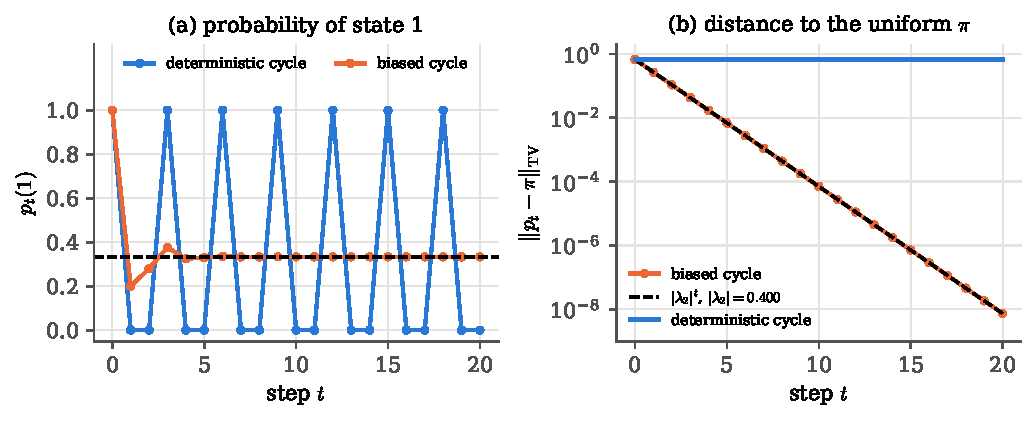
\includegraphics[width=\linewidth]{figures/ch09/cycles.pdf}
\caption{Two chains on a ring of three states, both with the uniform distribution as
equilibrium, started in state 1. (a) The deterministic cycle (blue) carries its spike round
forever; the biased cycle (orange) spirals in towards $\tfrac13$. (b) The distance to the
uniform distribution: constant for the deterministic cycle, and decaying as $0.4^t$ for the
biased one.}
\label{9a:fig:cycles}
\end{figure}

\paragraph{Reversibility as a movie run backwards.}
The name ``reversible'' has a literal meaning. In equilibrium, $X_t\sim\pi$, the probability of
seeing the step $i\to j$ is $\Prob(X_t=i,X_{t+1}=j)=\pi_ip_{ij}$, and of seeing $j\to i$ it is
$\pi_jp_{ji}$. Detailed balance says these are equal, so a film of the stationary chain has the
same statistics played forwards or backwards \srcref{Lambert}{§13.6.3}. For the biased cycle
the film run backwards shows a walker that prefers anticlockwise steps; you can tell the
direction of time.

\subsection{Continuous states}
\label{9a:sec:kernel}

Nothing changes for a continuous state space except that sums become integrals. The transition
matrix becomes a \newterm{transition kernel} $p(x,y)$, the density of the next state $y$ given
the current state $x$, with $\int p(x,y)\,\dd y=1$ \mainref{p.~413}. A density $f_t$ of walkers
moves to
\begin{equation}
  f_{t+1}(y)=\int f_t(x)\,p(x,y)\,\dd x
  \label{9a:eq:kernel-evolve}
\end{equation}
(the transition operator applied to $f_t$, \srcref{Lambert}{§13.6.1}), a density $f$ is
stationary if $f(y)=\int f(x)p(x,y)\,\dd x$, and detailed balance reads
$f(x)\,p(x,y)=f(y)\,p(y,x)$. The proof that it implies stationarity is
\eqref{9a:eq:db-implies} with integrals \mainref{p.~414, (24.7)}:
$\int f(x)p(x,y)\,\dd x=\int f(y)p(y,x)\,\dd x=f(y)\int p(y,x)\,\dd x=f(y)$.

\paragraph{Example: a Gaussian walker with a pull.}
Let the next state be $Y=\rho x+\sqrt{1-\rho^2}\,Z$ with $Z\sim\Normal(0,1)$ and $\abs\rho<1$,
so that $p(x,y)$ is the $\Normal(\rho x,1-\rho^2)$ density in $y$: a fraction $\rho$ of the
current position is kept and fresh noise is added. This is the \newterm{AR(1)} chain
(autoregressive of order 1), the discrete-time version of a Brownian particle in a harmonic
well (the Ornstein--Uhlenbeck process). Is $f=\Normal(0,1)$ stationary? Check detailed balance:
the exponent of $f(x)p(x,y)$ is
\begin{align*}
  -\frac{x^2}{2}-\frac{(y-\rho x)^2}{2(1-\rho^2)}
  &\eqby{1}-\frac{x^2(1-\rho^2)+y^2-2\rho xy+\rho^2x^2}{2(1-\rho^2)}
   \eqby{2}-\frac{x^2-2\rho xy+y^2}{2(1-\rho^2)} ,
\end{align*}
\begin{explain}
  \item Common denominator, and $(y-\rho x)^2=y^2-2\rho xy+\rho^2x^2$.
  \item The $\rho^2x^2$ terms cancel.
\end{explain}
which is symmetric under $x\leftrightarrow y$, and the prefactor
$1/(2\pi\sqrt{1-\rho^2})$ is symmetric too. So $f(x)p(x,y)=f(y)p(y,x)$: the AR(1) chain is
reversible with stationary law $\Normal(0,1)$. The joint law of two consecutive states in
equilibrium is the bivariate Gaussian with correlation $\rho$, the same whichever way round you
read it. We will watch this chain forget its starting point in \cref{9a:sec:diffusion}.
\section{Forgetting where you started}
\label{9a:sec:convergence}

Five weather forecasters use the same three-state weather chain \eqref{9a:eq:weather3}
(sunny, cloudy, rainy, with $p_{SS}=0.6$, $p_{CC}=0.7$, $p_{RR}=0.4$, rain clearing straight to
sun and no direct cloud--rain changes), but they disagree violently about today. One is certain
it is sunny, one certain it is cloudy, one certain it is raining; one has no idea and
says $(\tfrac13,\tfrac13,\tfrac13)$; one is $90\%$ sure of rain. Each forecasts day $t$ by
$p_t=p_0P^t$. \Cref{9a:fig:weather}a shows their forecasts of rain: wildly different on day 0,
nearly indistinguishable by day 5, all on the line $\pi_R=\tfrac16$ of the stationary
distribution \eqref{9a:eq:pi-weather3} soon after. The chain has forgotten where it started.

This is the property an MCMC run relies on. We cannot start a sampler from the target
distribution (if we could draw from it we would not need the sampler), so we start it
anywhere, and we need a guarantee that the start is forgotten, together with a rate.

\paragraph{The questions.}
\begin{enumerate}[itemsep=1pt]
  \item Does $p_t=p_0P^t$ converge to the same $\pi$ for every $p_0$?
  \item How fast does the memory of $p_0$ fade?
  \item What property of $P$ guarantees it?
\end{enumerate}

To answer ``how fast'' we need a distance between distributions.

\begin{workdef}[total-variation distance]
For two distributions $p,q$ on the same states,
\begin{equation}
  \norm{p-q}_{\rm TV}=\tfrac12\sum_i\abs{p_i-q_i}=\max_{A}\abs{p(A)-q(A)},
  \label{9a:eq:tv}
\end{equation}
where $A$ runs over all events \unpack{all subsets of states}. It is the largest disagreement
between $p$ and $q$ about the probability of any event, so it lies between 0 (identical) and
1 (no overlap at all). \emph{Operational recipe:} half the sum of absolute differences
(\pyname{tv} in \texttt{lib\_markov.py}).
\end{workdef}

The two expressions in \eqref{9a:eq:tv} agree. Let $A^*=\{i:p_i>q_i\}$. For any event $A$,
$p(A)-q(A)=\sum_{i\in A}(p_i-q_i)$ is largest when $A$ contains exactly the states where the
difference is positive, so the maximum is $p(A^*)-q(A^*)$ (and the most negative value is
$-(p(A^*)-q(A^*))$, at the complement). Because $\sum_i(p_i-q_i)=1-1=0$, the positive and the
negative differences have equal total size, and each is half of $\sum_i\abs{p_i-q_i}$.

\subsection{Two states: the whole story in one line}
\label{9a:sec:two-state}

Take a two-state chain with $a=p_{12}$, $b=p_{21}$ and stationary distribution
$\pi=(\frac{b}{a+b},\frac{a}{a+b})$ \eqref{9a:eq:pi-two}. Let $d_t=p_t(1)-\pi_1$ be the
forecaster's excess belief in state 1. Then
\begin{align}
  d_{t+1}=p_{t+1}(1)-\pi_1
  &\eqby{1}\bigl[p_t(1)(1-a)+(1-p_t(1))\,b\bigr]-\bigl[\pi_1(1-a)+(1-\pi_1)\,b\bigr]
  \nonumber\\
  &\eqby{2}(1-a-b)\bigl(p_t(1)-\pi_1\bigr)
   =\lambda\,d_t,
  \qquad \lambda\equiv1-a-b .
  \label{9a:eq:two-state-step}
\end{align}
\begin{explain}
  \item One step of \eqref{9a:eq:evolve} for the first component, for $p_t$ and for the
        stationary $\pi$ (for which one step changes nothing).
  \item Collect the terms in $p_t(1)$ and $\pi_1$: the constant $b$ cancels.
\end{explain}
So $d_t=\lambda^td_0$, and since $p_t(2)-\pi_2=-d_t$,
\begin{equation}
  p_t=\pi+\lambda^t\,(p_0-\pi),\qquad
  \norm{p_t-\pi}_{\rm TV}=\abs{\lambda}^t\,\norm{p_0-\pi}_{\rm TV} .
  \label{9a:eq:two-state-solution}
\end{equation}
The memory of the start decays geometrically with ratio $\abs\lambda=\abs{1-a-b}$, and
$\lambda$ is the second eigenvalue of $P$ (the trace of $P$ is $2-a-b=1+\lambda$). The two ways
for $\abs\lambda$ to equal 1 are exactly the failures of \cref{9a:sec:classify}: $a=b=0$, two
absorbing states and a reducible chain, which remembers its start forever; and $a=b=1$, a
deterministic flip with period 2, for which $\lambda=-1$ and the excess $d_t$ changes sign
every day without shrinking. Every other two-state chain forgets.

\paragraph{Example: Wasserman's weather.}
For \eqref{9a:eq:weather2}, $a=0.6$, $b=0.8$, so $\lambda=-0.4$ and $\pi=(\tfrac47,\tfrac37)$.
Starting on a sunny day, $d_0=1-\tfrac47=\tfrac37$, and
$p_t(\text{sunny})=\tfrac47+\tfrac37(-0.4)^t$: $1,\ 0.4,\ 0.64,\ 0.544,\dots$, the sequence
found by brute force in \cref{9a:sec:evolve}. The negative $\lambda$ explains the overshoot: a
sunny day makes cloud likely tomorrow, which makes sun likely the day after, and the
alternation damps by a factor $0.4$ a day.

\subsection{Many states: the eigenvalues of $P$}
\label{9a:sec:eigen}

For a $K$-state chain the role of $\lambda$ is played by the eigenvalues of $P$. Let us assume
that $P$ has $K$ independent eigenvectors (this is always true for a reversible chain, whose
eigenvalues were shown to be real in \cref{9a:sec:detailed-balance}; for the rest see the end of
this subsection). There are right eigenvectors, $Pv_k=\lambda_kv_k$ (columns), and left
eigenvectors, $\ell_kP=\lambda_k\ell_k$ (rows), with the same eigenvalues. A left and a right
eigenvector with different eigenvalues are orthogonal: $\ell_kPv_m$ equals both $\lambda_k\ell_kv_m$
and $\lambda_m\ell_kv_m$, so $\ell_kv_m=0$ when $\lambda_k\ne\lambda_m$. Label $\lambda_1=1$,
with right eigenvector $v_1=\mathbf1$ (rows sum to one) and left eigenvector $\ell_1=\pi$, and
order the rest by modulus, $\abs{\lambda_2}\ge\abs{\lambda_3}\ge\cdots$. Expand the starting
distribution in left eigenvectors, $p_0=\sum_kc_k\ell_k$; multiplying by $v_k$ and using the
orthogonality picks out one coefficient, $c_k=p_0v_k/(\ell_kv_k)$. Then
\begin{align}
  p_t=p_0P^t
  &\eqby{1}\sum_kc_k\,\ell_kP^t
   \eqby{2}\sum_kc_k\,\lambda_k^t\,\ell_k
   \eqby{3}\pi+\sum_{k\ge2}c_k\,\lambda_k^t\,\ell_k .
  \label{9a:eq:spectral}
\end{align}
\begin{explain}
  \item Expand $p_0$; the product is linear.
  \item Each $\ell_k$ is a left eigenvector, so $\ell_kP^t=\lambda_k^t\ell_k$.
  \item $\lambda_1=1$, $\ell_1=\pi$ and
        $c_1=p_0\mathbf1/(\pi\mathbf1)=1/1=1$: every probability vector contains exactly one
        unit of the stationary distribution.
\end{explain}
Every other component is multiplied by $\lambda_k^t$ each step. If $\abs{\lambda_k}<1$ for all
$k\ge2$, all of them die and $p_t\to\pi$ from any start. At late times the slowest one
dominates,
\begin{equation}
  \norm{p_t-\pi}_{\rm TV}\simeq C\,\abs{\lambda_2}^t,
  \qquad
  \ln\norm{p_t-\pi}_{\rm TV}\simeq\ln C+t\ln\abs{\lambda_2},
  \label{9a:eq:lambda2-rate}
\end{equation}
a straight line of slope $\ln\abs{\lambda_2}$ on a log plot. The number of steps for the
memory to fall by a factor $e$ is the \newterm{relaxation time}
$t_{\rm rel}=-1/\ln\abs{\lambda_2}$, and $1-\abs{\lambda_2}$ is called the \newterm{spectral
gap}. This is exactly the physics of normal modes in a damped system: the initial condition is
a superposition of modes, each decays at its own rate, and after a while only the slowest one
is visible.

\paragraph{Why $\abs\lambda\le1$, and why only one eigenvalue equals 1.}
This is the Perron--Frobenius theorem for stochastic matrices, and for our purposes it has a
two-line proof. Take a right eigenvector, $Pv=\lambda v$, and look at its largest entry in
modulus, at state $i^*$. Row $i^*$ of $Pv$ is an \emph{average} of the entries of $v$ with
weights $p_{i^*j}\ge0$ that sum to one, and an average cannot exceed the largest thing being
averaged:
\begin{align}
  \abs\lambda\,\abs{v_{i^*}}
  =\abs{(Pv)_{i^*}}
  &\eqby{1}\Bigl|\sum_jp_{i^*j}v_j\Bigr|
   \relby{2}{\le}\sum_jp_{i^*j}\abs{v_j}
   \relby{3}{\le}\sum_jp_{i^*j}\abs{v_{i^*}}
   \eqby{4}\abs{v_{i^*}} .
  \label{9a:eq:pf}
\end{align}
\begin{explain}
  \item Definition of the matrix--vector product.
  \item Triangle inequality.
  \item $\abs{v_j}\le\abs{v_{i^*}}$ by the choice of $i^*$.
  \item Row $i^*$ sums to one.
\end{explain}
So $\abs\lambda\le1$. Now suppose the chain is ergodic, so that some power $P^m$ has all entries
positive (\cref{9a:sec:period}), and apply the same argument to $P^m$, whose eigenvalue for $v$
is $\lambda^m$. If $\abs{\lambda}=1$, both inequalities in \eqref{9a:eq:pf} must be equalities.
With every weight $p_{i^*j}(m)$ positive, equality in (3) forces $\abs{v_j}=\abs{v_{i^*}}$ for
\emph{all} $j$, and equality in the triangle inequality (2) forces all the $v_j$ to have the same
phase. So $v$ is constant, $v\propto\mathbf1$, and then $Pv=v$ says $\lambda=1$. Hence for an ergodic chain the eigenvalue 1 belongs only to the constant vector and
every other eigenvalue has $\abs{\lambda_k}<1$. The failures are again the ones of
\cref{9a:sec:classify}: the deterministic 3-cycle has the eigenvalues $1,e^{\pm2\pi i/3}$, all of
modulus 1, which rotate the spike forever; a chain with two closed classes has the eigenvalue 1
twice, one stationary distribution living on each class.

\emph{When there are not enough eigenvectors.} The expansion \eqref{9a:eq:spectral} assumed
$K$ independent eigenvectors. A matrix can fall short of that, and the simplest example shows
what changes. Take the $2\times2$ block
\begin{equation*}
  B=\begin{pmatrix}\lambda&1\\0&\lambda\end{pmatrix},\qquad
  B^t=\begin{pmatrix}\lambda^t&t\lambda^{t-1}\\0&\lambda^t\end{pmatrix},
\end{equation*}
which has the single eigenvector $(1,0)^{\mathsf T}$. The formula for $B^t$ holds at $t=1$, and
multiplying it by $B$ once more gives the off-diagonal entry $\lambda^t+t\lambda^{t-1}\lambda
=(t+1)\lambda^t$, so it holds for all $t$. The power still decays like $\abs\lambda^t$, only
with an extra factor $t$, which a geometric decay overwhelms. Every square matrix can be brought
to blocks of this kind (its Jordan form), and a block of size $r+1$ gives factors up to $t^r$;
the decay is again geometric with ratio $\abs{\lambda_2}$, so the conclusion is unchanged. The
general block is not worked out here, and nothing below depends on it: the Doeblin argument of
\cref{9a:sec:doeblin} proves geometric forgetting without any eigenvectors.

\paragraph{Example: the three-state weather chain, exactly.}
Take the three-state weather chain \eqref{9a:eq:weather3} (sunny, cloudy, rainy), with
$\pi=(\tfrac12,\tfrac13,\tfrac16)$ from \eqref{9a:eq:pi-weather3}, and find all of its
eigenvalues and eigenvectors by hand.

\emph{The eigenvalues.} The sum of the eigenvalues is the trace, $0.6+0.7+0.4=1.7$, and their
product is the determinant. Expanding along the first row, each entry times the $2\times2$
determinant left when its row and column are struck out,
\begin{align*}
  \det P
  &=0.6\begin{vmatrix}0.7&0\\0&0.4\end{vmatrix}
   -0.2\begin{vmatrix}0.3&0\\0.6&0.4\end{vmatrix}
   +0.2\begin{vmatrix}0.3&0.7\\0.6&0\end{vmatrix}
   =0.6(0.28)-0.2(0.12)+0.2(-0.42)=0.06 .
\end{align*}
With $\lambda_1=1$ the other two satisfy $\lambda_2+\lambda_3=0.7$ and
$\lambda_2\lambda_3=0.06$, the roots of $\lambda^2-0.7\lambda+0.06=0$: $\lambda_2=0.6$ and
$\lambda_3=0.1$.

\emph{The right eigenvectors.} For $\lambda=0.6$ the equation $(P-0.6\,\Id)v=0$ is three
row equations,
\begin{equation*}
  0.2v_2+0.2v_3=0,\qquad 0.3v_1+0.1v_2=0,\qquad 0.6v_1-0.2v_3=0 .
\end{equation*}
The third gives $v_3=3v_1$, the second $v_2=-3v_1$, and the first is then satisfied
($-0.6v_1+0.6v_1=0$), as it must be for an eigenvalue. Choosing $v_1=1$ gives
$v_2=(1,-3,3)^{\mathsf T}$. For $\lambda=0.1$ the rows read $0.5v_1+0.2v_2+0.2v_3=0$,
$0.3v_1+0.6v_2=0$ and $0.6v_1+0.3v_3=0$, so $v_2=-\tfrac12v_1$ and $v_3=-2v_1$; with $v_1=2$,
$v_3=(2,-1,-4)^{\mathsf T}$ (the first row checks: $1-0.2-0.8=0$).

\emph{The left eigenvectors from reversibility.} The chain satisfies detailed balance
(\cref{9a:sec:detailed-balance}), and that turns each right eigenvector into a left one. Define
$\ell(i)=\pi_iv(i)$, each entry of $v$ weighted by the stationary probability. Then
\begin{align*}
  (\ell P)_j
  &\eqby{1}\sum_i\pi_iv_i\,p_{ij}
   \eqby{2}\sum_i\pi_jp_{ji}\,v_i
   \eqby{3}\pi_j\,(Pv)_j
   \eqby{4}\lambda\,\pi_jv_j=\lambda\,\ell_j .
\end{align*}
\begin{explain}
  \item Row vector times matrix, with $\ell_i=\pi_iv_i$.
  \item Detailed balance, $\pi_ip_{ij}=\pi_jp_{ji}$.
  \item $\pi_j$ does not depend on $i$; what is left is row $j$ of $Pv$.
  \item $v$ is a right eigenvector.
\end{explain}
So
\begin{align*}
  v_2&=(1,-3,3)^{\mathsf T}, & \ell_2&=\bigl(\tfrac12,-1,\tfrac12\bigr), & \ell_2v_2&=5,\\
  v_3&=(2,-1,-4)^{\mathsf T}, & \ell_3&=\bigl(1,-\tfrac13,-\tfrac23\bigr), & \ell_3v_3&=5.
\end{align*}
(Check one: the first entry of $\ell_2P$ is $\tfrac12(0.6)-1(0.3)+\tfrac12(0.6)=0.3=0.6\cdot\tfrac12$.)
For the forecaster certain of rain, $p_0=(0,0,1)$, so $c_2=p_0v_2/5=\tfrac35$ and
$c_3=p_0v_3/5=-\tfrac45$, and \eqref{9a:eq:spectral} becomes
\begin{equation}
  p_t=\bigl(\tfrac12,\tfrac13,\tfrac16\bigr)
      +\tfrac35\,(0.6)^t\,\bigl(\tfrac12,-1,\tfrac12\bigr)
      -\tfrac45\,(0.1)^t\,\bigl(1,-\tfrac13,-\tfrac23\bigr).
  \label{9a:eq:weather-exact}
\end{equation}
At $t=0$ this is $(0,0,1)$, as it must be. The $0.1^t$ mode is gone within two or three days;
after that $\norm{p_t-\pi}_{\rm TV}\simeq\tfrac35(0.6)^t\cdot\tfrac12(\tfrac12+1+\tfrac12)
=\tfrac35(0.6)^t$. On day 10 this predicts $\NineAWTVTenPred$, and the exact distance is
$\NineAWTVTen$; by day 20 it is $\NineAWTVTwenty$. Fitting a straight line to $\ln\norm{p_t-\pi}$
over days 10--30 gives slope $\NineAWSlope$, against $\ln0.6=\NineAWLnLam$
(\cref{9a:fig:weather}b). All five forecasters have the same slope; they differ only in the
constant $C$, which is the size of their initial error along $\ell_2$. The uniform forecaster
starts closest and stays closest. Simulating $\NineAWWalkers$ independent weather histories from
a rainy day reproduces the exact curve until it hits the Monte Carlo floor
$\approx\NineAWMCFloor$, the typical distance between $\pi$ and a histogram of that many draws
from $\pi$.

\begin{figure}[htbp]
\centering
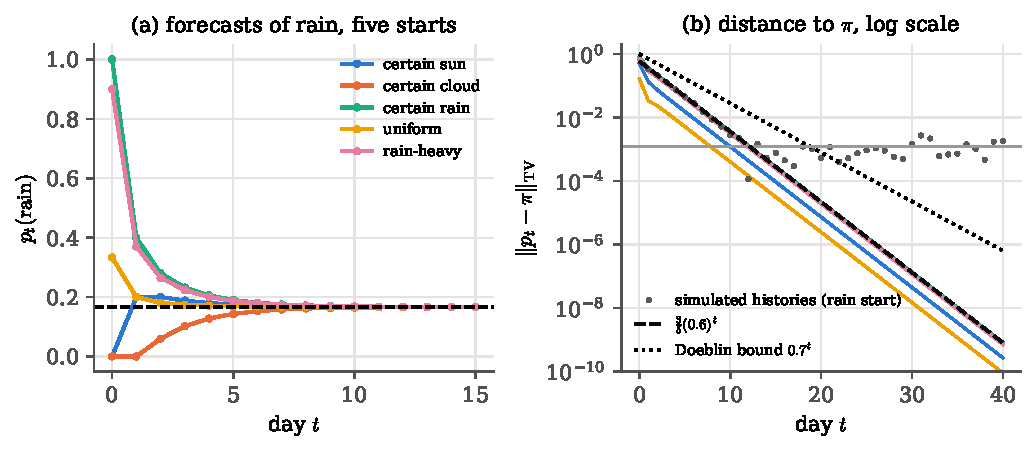
\includegraphics[width=\linewidth]{figures/ch09/weather_convergence.pdf}
\caption{Five forecasters with very different beliefs about day 0, one weather chain. (a) Their
forecasts of rain converge to $\pi_R=\frac16$ (dashed) within a few days. (b) The total-variation
distance to $\pi$ on a log scale: after a short transient from the fast $0.1^t$ mode, every curve
is a straight line of slope $\ln0.6$, parallel to $\frac35(0.6)^t$ (dashed). Grey dots are
$2\times10^5$ simulated histories started on a rainy day; they follow the exact curve down to
the sampling-noise floor (horizontal line). The dotted line is the Doeblin bound $0.7^t$ of
\cref{9a:sec:doeblin}, which lies above every curve.}
\label{9a:fig:weather}
\end{figure}

\begin{keyidea}[A finite ergodic chain forgets its start]
If a finite chain is irreducible and aperiodic, it has exactly one stationary distribution
$\pi$, and for every initial distribution $p_0$, $\norm{p_0P^t-\pi}_{\rm TV}\to0$
geometrically. The rate is set by the second-largest eigenvalue modulus:
$\norm{p_t-\pi}_{\rm TV}\simeq C\abs{\lambda_2}^t$.
\end{keyidea}

\subsection{The easy-to-see proof: a contraction}
\label{9a:sec:doeblin}

The eigenvalue argument gives the exact rate, but it needs the eigenvectors. There is a cruder
argument that needs nothing, works directly with probability, and proves convergence,
existence and uniqueness of $\pi$ at once. It goes back to Doeblin.

\paragraph{The idea.} Look at the rows of the weather matrix \eqref{9a:eq:weather3} as three
forecasts for tomorrow, one for each kind of today (\cref{9a:fig:doeblin}). Whatever today is,
tomorrow is sunny with probability at least $0.3$ (the smallest entry of the first column). That
$0.3$ is common to all three forecasts: it does not depend on today at all. So we may think of
tomorrow's weather as drawn in two stages. With probability $\delta=0.3$, ignore today
completely and draw tomorrow from a fixed distribution $\nu$ (here, sun for certain). With
probability $1-\delta=0.7$, draw it from what is left of today's row. Whenever the first branch
is taken, the memory of today is wiped out. After $t$ days the memory survives only if the
second branch was taken every time, which has probability $0.7^t$.

\begin{figure}[htbp]
\centering
\begin{tikzpicture}[x=9cm,y=0.75cm]
  \foreach \r/\lab/\s/\c in {2/S/0.6/0.2, 1/C/0.3/0.7, 0/R/0.6/0.0} {
    \pgfmathsetmacro{\rr}{1-\s-\c}
    \fill[tangentgreen!35] (0,\r) rectangle (0.3,\r+0.7);
    \fill[formblue!20] (0.3,\r) rectangle (\s,\r+0.7);
    \fill[fibreorange!30] (\s,\r) rectangle ({\s+\c},\r+0.7);
    \fill[bdryred!25] ({\s+\c},\r) rectangle (1,\r+0.7);
    \draw[softgray] (0,\r) rectangle (1,\r+0.7);
    \node[anchor=east,font=\small] at (-0.01,\r+0.35) {today \lab};
  }
  \draw[thick,tangentgreen!60!black,dashed] (0.3,-0.25) -- (0.3,2.95);
  \node[font=\footnotesize,anchor=south] at (0.15,2.95) {shared: $\delta=0.3$};
  \node[font=\footnotesize,anchor=north] at (0.3,-0.25) {sun};
  \node[font=\footnotesize,anchor=north] at (0.8,-0.25) {cloud / rain (row-dependent)};
\end{tikzpicture}
\caption{The rows of the weather matrix as stacked bars: tomorrow's sun (green and blue),
cloud (orange) and rain (red), for each kind of today. The green part, a probability $0.3$ of
sun, is the same in every row; the rest depends on today. Each day, the shared part erases the
dependence on the past with probability $\delta=0.3$.}
\label{9a:fig:doeblin}
\end{figure}

\paragraph{The calculation.} Define the \newterm{Doeblin coefficient}
$\delta=\sum_j\min_ip_{ij}$, the total mass that all rows have in common, and suppose
$\delta>0$. Then $\nu_j=\min_ip_{ij}/\delta$ is a probability vector, and
$R=(P-\delta\,\mathbf1\nu)/(1-\delta)$ is a stochastic matrix (its entries are non-negative
because $p_{ij}\ge\min_kp_{kj}$, and its rows sum to $(1-\delta)/(1-\delta)=1$). So
\begin{equation}
  P=\delta\,\mathbf1\nu+(1-\delta)\,R,
  \label{9a:eq:doeblin-split}
\end{equation}
where $\mathbf1\nu$ is the matrix with every row equal to $\nu$. Take any two distributions $p$
and $q$:
\begin{align}
  \norm{pP-qP}_{\rm TV}
  &\eqby{1}\tfrac12\bigl\lVert\delta\,(p-q)\mathbf1\,\nu+(1-\delta)(p-q)R\bigr\rVert_1
   \eqby{2}(1-\delta)\,\tfrac12\norm{(p-q)R}_1 \nonumber\\
  &\relby{3}{\le}(1-\delta)\,\tfrac12\norm{p-q}_1
   =(1-\delta)\,\norm{p-q}_{\rm TV} .
  \label{9a:eq:contraction}
\end{align}
\begin{explain}
  \item Insert \eqref{9a:eq:doeblin-split}; $\norm{x}_1=\sum_j\abs{x_j}$.
  \item $(p-q)\mathbf1=\sum_ip_i-\sum_iq_i=0$: the shared part sends both distributions to the
        same place, so it cancels in the difference.
  \item A stochastic matrix cannot increase the $\ell_1$ norm:
        $\sum_j\abs{\sum_ix_iR_{ij}}\le\sum_j\sum_i\abs{x_i}R_{ij}=\sum_i\abs{x_i}$, using the
        triangle inequality and then the row sums of $R$.
\end{explain}
One step of the chain shrinks the distance between any two distributions by at least the factor
$1-\delta$. Three consequences follow at once.
\begin{itemize}[itemsep=1pt]
  \item \emph{Uniqueness.} If $\pi$ and $\pi'$ were both stationary,
        $\norm{\pi-\pi'}=\norm{\pi P-\pi'P}\le(1-\delta)\norm{\pi-\pi'}$, which forces
        $\norm{\pi-\pi'}=0$.
  \item \emph{Existence.} The sequence $p_0,p_0P,p_0P^2,\dots$ has steps that shrink
        geometrically, so it is a Cauchy sequence and converges; its limit is unchanged by one
        more step, so it is stationary. (This is the contraction-mapping theorem.)
  \item \emph{Forgetting, with a guaranteed rate.} Taking $q=\pi$ and iterating,
        \begin{equation}
          \norm{p_0P^t-\pi}_{\rm TV}\le(1-\delta)^t\,\norm{p_0-\pi}_{\rm TV}\le(1-\delta)^t .
          \label{9a:eq:doeblin-bound}
        \end{equation}
\end{itemize}

\paragraph{Example: two states, where the bound is exact.}
For the two-state chain, $\delta=\min(1-a,b)+\min(a,1-b)$. If $a+b\le1$ then $1-a\ge b$ and
$1-b\ge a$, so $\delta=a+b$ and $1-\delta=1-a-b$. If $a+b>1$ the minima are $1-a$ and $1-b$, so
$1-\delta=a+b-1$. Either way $1-\delta=\abs{1-a-b}=\abs\lambda$: for two states the contraction
factor is exactly the eigenvalue modulus, and \eqref{9a:eq:doeblin-bound} is the exact solution
\eqref{9a:eq:two-state-solution}. For Wasserman's weather,
$\delta=\min(0.4,0.8)+\min(0.6,0.2)=0.6$ and $1-\delta=0.4=\abs{-0.4}$.

\paragraph{Example: three states, where it is only a bound.}
For the three-state weather chain the column minima are $0.3$, $0$ and $0$, so
$\delta=\NineAWDelta$ and the guaranteed factor is $0.7$ per day, against the true $0.6$
(\cref{9a:fig:weather}b, dotted line). The bound is honest but pessimistic: it only uses the part
of the rows that is literally identical, while the eigenvalue sees all the averaging.

\paragraph{When no column is shared.}
For the politician, no island can be reached from every island in one night, so every column of
\eqref{9a:eq:politician-matrix} has a zero and $\delta=0$. The argument then applies to $P^m$
instead of $P$: for an ergodic chain some power $P^m$ is strictly positive (\cref{9a:sec:period}),
so its Doeblin coefficient $\delta_m$ is positive, and the distance shrinks by $1-\delta_m$ every
$m$ steps.

\emph{The seven islands.} After three nights, can every island have sent the politician to
island 4? From island 1 the only way is east, east, east, with probability
$\tfrac12\cdot\tfrac12\cdot\tfrac12=\tfrac18$; from island 7 it is west, west, west, with
probability $\tfrac37\cdot\tfrac5{12}\cdot\tfrac25=\tfrac1{14}$. The islands nearer to 4 get
there in fewer moves and must spend the remaining nights somewhere, which they can because
every island has a refused proposal, $p_{\theta\theta}=1/(2\theta)>0$, by
\eqref{9a:eq:politician-rows}. Adding the probabilities of all such three-night paths gives
column 4 of $P^3$, from islands $1,\dots,7$:
\begin{equation*}
  \bigl(0.125,\ 0.135,\ 0.309,\ 0.150,\ 0.254,\ 0.051,\ 0.071\bigr).
\end{equation*}
Every entry is positive, and the smallest, $0.051$ from island 6 (two moves plus one wasted
night on an island that rarely refuses), is the mass that all rows of $P^3$ share in column 4.
No other column of $P^3$ is positive in every row (island 1 cannot reach island 5 or beyond in
three nights, island 7 cannot reach 3 or below), so $\delta_3\approx0.05$. Longer blocks share
more:
\begin{center}
\small
\begin{tabular}{@{}lcccccc@{}}
  \toprule
  block length $m$ & 1 & 2 & 3 & 4 & 5 & 6\\
  \midrule
  $\delta_m$ & 0 & 0 & 0.051 & 0.152 & 0.229 & 0.316\\
  \bottomrule
\end{tabular}
\end{center}
At $m=6$ every column has a positive minimum, so $P^6$ is strictly positive. Geometric
forgetting holds; only the guaranteed rate is per block of $m$ steps, for example a factor
$1-0.316$ every six days.

\emph{The actual rate.} It is again $\abs{\lambda_2}$, which is $\NineAIslLamTwo$ for the
politician. The memory falls as $\abs{\lambda_2}^t$, so it halves after the number of days $t$ with
$\abs{\lambda_2}^{t}=\tfrac12$, that is $t=\ln2/(-\ln\abs{\lambda_2})=\ln2/(-\ln\NineAIslLamTwo)
\approx6$ days, slower than the weather, because he can move only one island at a time.

\subsection{Coupling: two walkers who meet}
\label{9a:sec:coupling}

The two-stage picture of the Doeblin step has a vivid probabilistic version, which turns the
inequality into a story about two walkers. Walker A starts from our arbitrary $p_0$. Walker B
starts from the stationary $\pi$, so B's distribution is $\pi$ on every day. Let them move
together in a correlated way, each one still obeying the chain $P$ on its own, and arrange that
once they stand on the same state they move together forever. Let $T$ be the day they first
meet. After $T$ the two walkers are identical, so for any event $A$,
\begin{align}
  \abs{\Prob(X^A_t\in A)-\Prob(X^B_t\in A)}
  &\eqby{1}\abs{\Prob(X^A_t\in A,\,T>t)-\Prob(X^B_t\in A,\,T>t)}
   \relby{2}{\le}\Prob(T>t),
  \label{9a:eq:coupling}
\end{align}
\begin{explain}
  \item Split each probability according to whether $T\le t$ or $T>t$. On $T\le t$ the two
        walkers are at the same place, so those parts are equal and cancel.
  \item Both remaining terms lie between 0 and $\Prob(T>t)$, so their difference does too.
\end{explain}
and, since $X^B_t\sim\pi$, maximising over $A$ gives the \newterm{coupling inequality}
$\norm{p_t-\pi}_{\rm TV}\le\Prob(T>t)$. Forgetting the start is the same as meeting a walker
who never had one to forget.

The Doeblin split \eqref{9a:eq:doeblin-split} tells us how to make them meet.

\emph{The construction.} Each day, flip one coin, shared by both walkers, that comes up heads
with probability $\delta$. On heads, draw one state from $\nu$ and move \emph{both} walkers
there. On tails, each walker draws its next state from its own row of $R$, independently of the
other. Once they stand on the same state, let them use the same random numbers from then on, so
they never separate.

\emph{Each walker on its own is still the chain $P$.} Look at walker A alone, standing at $i$.
It goes to $j$ either by heads and then $\nu$ choosing $j$, or by tails and then row $i$ of $R$
choosing $j$:
\begin{equation*}
  \Prob(\text{A moves }i\to j)=\delta\,\nu_j+(1-\delta)\,R_{ij}=p_{ij},
\end{equation*}
which is exactly row $i$ of \eqref{9a:eq:doeblin-split}. The same holds for B, and also after
the meeting, since then both follow one walker's moves. So the coupling changes how the two
walkers are correlated but not how either moves, and $X^B_t\sim\pi$ on every day, as the
coupling inequality needs.

\emph{The meeting time.} Every heads day ends with the walkers together, so they can still be
apart on day $t$ only if all $t$ coins came up tails: $\Prob(T>t)\le(1-\delta)^t$, which is
\eqref{9a:eq:doeblin-bound} again, now as a statement about meeting times. The bound can be
sharpened a little at the start. A and B may already stand on the same state on day 0; with
their starting draws arranged to agree as often as possible, this happens with probability
$\sum_i\min(p_0(i),\pi_i)$. For A starting on a rainy day this is $\pi_R$, so the two are apart
on day 0 with probability $1-\pi_R$, and $\Prob(T>t)\le(1-\delta)^t(1-\pi_R)$.

The script \texttt{05\_coupling.py} runs $\NineACoupWalkers$ pairs from a rainy
day (A) and from $\pi$ (B), once with this Doeblin coupling and once with the naive coupling in
which the two walkers move independently until they happen to meet
(\cref{9a:fig:coupling}). On day 10 the exact distance is $\NineACoupTVTen$; the probability of
not having met is $\NineACoupDoeTen$ for the Doeblin coupling and $\NineACoupIndTen$ for
independent moves; and the guaranteed bound $(0.7)^{10}(1-\pi_R)$ is $\NineACoupBoundTen$. Each coupling gives a valid
upper bound on the distance; a cleverer coupling gives a tighter one.

\begin{figure}[htbp]
\centering
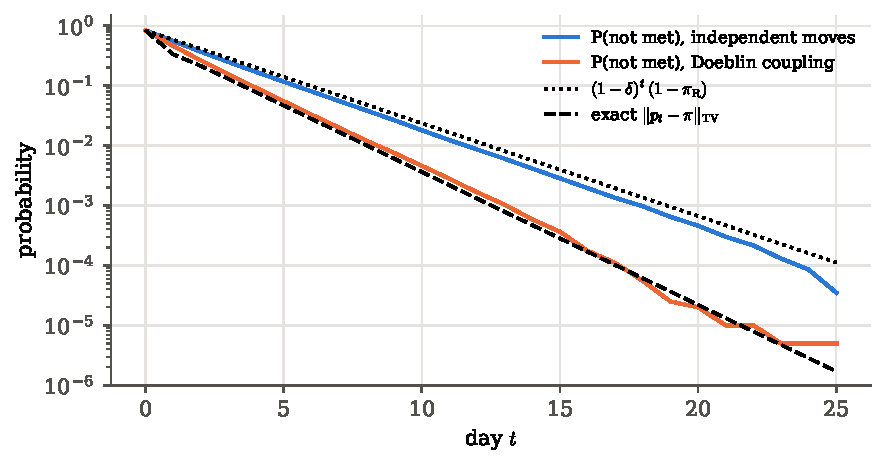
\includegraphics[width=0.8\linewidth]{figures/ch09/coupling.pdf}
\caption{Coupling a walker started on a rainy day with one started from the stationary
distribution. The probability that they have not yet met, for walkers moving independently
(blue) and for the Doeblin coupling that sometimes forces them onto the same state (orange),
always lies above the true distance $\norm{p_t-\pi}_{\rm TV}$ (dashed), and the Doeblin coupling
lies below its guaranteed bound $(1-\delta)^t(1-\pi_R)$ (dotted).}
\label{9a:fig:coupling}
\end{figure}

\begin{pitfall}[A bound is not a rate]
$(1-\delta)^t$ and $\Prob(T>t)$ guarantee forgetting; they do not measure it. The actual
decay of $\norm{p_t-\pi}$ is $\abs{\lambda_2}^t$, which can be much faster. In the other
direction, a chain can look converged long before it is: a walker trapped in one of two
well-separated regions has $\abs{\lambda_2}$ just below 1, a tiny Doeblin coefficient, and a
histogram that looks perfectly stable for a long time while it misses half of the target.
\end{pitfall}
\section{One long walk is a sample: the ergodic theorem}
\label{9a:sec:ergodic}

\Cref{9a:sec:convergence} was about a crowd: the histogram of many independent walkers on day
$t$ approaches $\pi$. An MCMC run is not a crowd. It is one walker (or a handful), followed for a
long time, and what we use is its diary: the fraction of steps it spent in each region, or the
average of some quantity $g$ over all the steps. One politician, followed for $\NineAIslDays$
days, spent his days in proportions within $\NineAIslMaxDev$ of $\theta/28$
(\cref{9a:fig:island-traj}b). Why should a single walker's diary reproduce the crowd's
equilibrium? The successive entries in the diary are not independent, so the ordinary law of
large numbers of \cref{ch:03} does not apply.

\paragraph{The questions.}
\begin{enumerate}[itemsep=1pt]
  \item Does the fraction of time one walker spends in state $j$ converge to $\pi_j$, and the
        average of $g(X_t)$ along the walk to $\E_\pi g=\sum_jg(j)\pi_j$?
  \item How accurate is the average after $N$ steps, given that the steps are correlated?
\end{enumerate}
The first question is the oscillator's question of \cref{9a:sec:oscillator}, time average
versus ensemble average, now for a random dynamics.

\begin{keyidea}[Ergodic theorem for Markov chains]
For an irreducible, ergodic Markov chain with stationary distribution $\pi$, started anywhere,
and for any bounded function $g$ of the state,
\begin{equation}
  \frac1N\sum_{n=1}^Ng(X_n)\;\xrightarrow[N\to\infty]{}\;\E_\pi(g)=\sum_jg(j)\,\pi_j
  \qquad\text{with probability one}
  \label{9a:eq:ergodic}
\end{equation}
\mainref{p.~391, Thm~23.25}. The time average along one walk equals the average over the
stationary ensemble.
\end{keyidea}

It is a law of large numbers for dependent variables, and the iid law is the special case of a
chain that ignores its present state \srcref{CasellaBerger}{§5.8.5}. Markov introduced his chains for this very purpose: the law of large numbers does not need independence, only forgetting (in 1913 he marked the two-hundredth anniversary of the law with a celebration of his own \srcref{Lambert}{§12.9}). It is the reason MCMC
works at all: estimate any posterior expectation by averaging along the chain
\mainref{p.~411}. Two arguments make it believable at our level: one counts returns, the other
computes the variance.

\subsection{Why: counting returns}
\label{9a:sec:kac}

Take $g$ to be the indicator of one state $j$, so that the time average is the fraction of time
spent in $j$. Every time the walker arrives at $j$, the Markov property says the future is a
fresh copy of the chain started at $j$, independent of how it got there. So the waiting times
between successive visits, $T^{(1)},T^{(2)},\dots$, are independent copies of the return time
$T_{jj}$, with mean $m_j$ (\cref{9a:sec:recurrence}). After the $k$th visit the elapsed time is
$T^{(1)}+\dots+T^{(k)}$ (plus the time to the first visit, which is finite and does not grow with
$k$), so
\begin{align}
  \frac{\text{visits to }j\text{ in }n\text{ steps}}{n}
  &\eqby{1}\frac{k}{T^{(1)}+\dots+T^{(k)}}
  \eqby{2}\Bigl(\frac{T^{(1)}+\dots+T^{(k)}}{k}\Bigr)^{-1}
  \;\xrightarrow[k\to\infty]{}\;\frac1{m_j}.
  \label{9a:eq:kac-frac}
\end{align}
\begin{explain}
  \item Choose $n$ at the $k$th visit; between visits the count does not change, and this
        changes the fraction by at most $1/k$.
  \item The ordinary law of large numbers for the iid return times: their average tends to
        $m_j$.
\end{explain}
The long-run fraction of time in $j$ exists and equals $1/m_j$, whatever the start, since an
irreducible finite chain reaches $j$ from anywhere.

\emph{Which number is $1/m_j$?} Now run the same walker from a different start: draw $X_0$
from a stationary distribution $\pi$ (one exists for every finite chain,
\cref{9a:sec:stationary}). Then $p_t=\pi$ on every day, and the \emph{expected} fraction of time
in $j$ over $n$ steps is exactly
\begin{equation*}
  \E\Bigl(\frac{\text{visits to }j\text{ in }n\text{ steps}}{n}\Bigr)=\frac1n\sum_{t=1}^n\Prob(X_t=j)
  =\frac1n\sum_{t=1}^n\pi_j=\pi_j
\end{equation*}
for every $n$ (the expectation of a count of visits is the sum of the probabilities of a
visit, as in \eqref{9a:eq:visits}). The fraction itself tends to $1/m_j$ with probability one,
and it always lies between 0 and 1. A sequence of random variables that stays between fixed
bounds and converges with probability one also has converging expectations (the bounded
convergence theorem: no rare, huge values can hold the mean away from the limit). So the
constant expectation $\pi_j$ equals the limit $1/m_j$, which gives \newterm{Kac's formula}
\begin{equation}
  \pi_j=\frac{1}{m_j}:
  \label{9a:eq:kac}
\end{equation}
the equilibrium probability of a state is one over its mean recurrence time. A rare state is one
that is revisited only after long excursions. Two by-products come free. The argument never
asked whether $p_t$ converges from other starts, so it holds for periodic chains too. And since
$m_j$ is fixed by the chain, any stationary distribution must equal $(1/m_1,\dots,1/m_K)$:
an irreducible finite chain has only one.

\emph{From one state to any function.} On a finite state space any function $g$ is a sum of
indicators, $g(x)=\sum_jg(j)\,I(x=j)$, so its time average is a weighted sum of time fractions,
\begin{equation*}
  \frac1N\sum_{n=1}^Ng(X_n)=\sum_jg(j)\times\Bigl(\text{fraction of the }N\text{ steps spent in }j\Bigr)
  \;\xrightarrow[N\to\infty]{}\;\sum_jg(j)\,\pi_j=\E_\pi(g),
\end{equation*}
each fraction tending to $\pi_j=1/m_j$ and the finite sum following term by term. That is
\eqref{9a:eq:ergodic}.

\paragraph{Example: how long until it rains again?}
For the three-state weather chain $\pi_R=\tfrac16$, so the mean time from one rainy day to the
next is 6 days. In a simulated history of $\NineAErgLong$ days the average gap between rainy days
is $\NineAErgRainGap$. For the politician, $\pi_1=\tfrac1{28}$: having left island 1, he is back
there on average 28 nights later.

\paragraph{Example: the cycle.}
The deterministic 3-cycle of \cref{9a:sec:not-convergent} returns to each state after exactly 3
steps, so $m_j=3$ and the time fractions are exactly $\tfrac13=\pi_j$. Yet $p_t$ never
converges. The return argument used irreducibility and positive recurrence, but not
aperiodicity. That is a general fact: periodicity spoils the convergence of the distribution at
a fixed time, not the convergence of time averages. The tilted die that always moves to a
neighbouring face (\cref{9a:sec:period}) has period 2, and its average face value still tends to
3.5.

\subsection{How accurate: the variance of a time average}
\label{9a:sec:time-average-variance}

Suppose the chain has already reached equilibrium, $X_1\sim\pi$, so that every $X_t$ has the
same distribution and the covariance $C_k=\Cov\bigl(g(X_t),g(X_{t+k})\bigr)$ depends only on the
lag $k$. Write $\bar g_N=\frac1N\sum_{t=1}^Ng(X_t)$, $\sigma^2=C_0$, and
$\rho_k=C_k/C_0$ for the autocorrelation at lag $k$. Then
\begin{align}
  \Var(\bar g_N)
  &\eqby{1}\frac1{N^2}\sum_{s=1}^N\sum_{t=1}^NC_{\abs{s-t}}
   \eqby{2}\frac1{N^2}\Bigl[NC_0+2\sum_{k=1}^{N-1}(N-k)\,C_k\Bigr] \nonumber\\
  &\eqby{3}\frac{\sigma^2}{N}\Bigl[1+2\sum_{k=1}^{N-1}\Bigl(1-\frac kN\Bigr)\rho_k\Bigr]
   \;\simeq\;\frac{\sigma^2}{N}\,\tau,
   \qquad \tau\equiv1+2\sum_{k=1}^\infty\rho_k .
  \label{9a:eq:var-time-average}
\end{align}
\begin{explain}
  \item Variance of a sum is the sum of all covariances (\cref{ch:01}), with stationarity.
  \item There are $N$ pairs with $s=t$ and $2(N-k)$ ordered pairs with $\abs{s-t}=k$.
  \item Factor out $N$; for $N$ much larger than the correlation length, $k/N\to0$ in the terms
        that matter, and the sum extends to infinity.
\end{explain}
\emph{Is $\tau$ finite?} The covariances can be computed from $P$. Centre $g$ on its
equilibrium mean, $g_c=g-\E_\pi g$. Given $X_t=i$, the expected value of $g_c$ after $k$ more
steps is $\sum_jp_{ij}(k)g_c(j)=(P^kg_c)(i)$, so averaging over $X_t\sim\pi$,
\begin{equation*}
  C_k=\E\bigl[g_c(X_t)\,g_c(X_{t+k})\bigr]=\sum_i\pi_i\,g_c(i)\,(P^kg_c)(i).
\end{equation*}
Expand $g_c$ in the right eigenvectors of $P$, $g_c=\sum_mb_mv_m$, the same expansion as
\eqref{9a:eq:spectral} with columns in place of rows (assuming, as there, a full set of
eigenvectors). There is no $m=1$ term, since $v_1=\mathbf1$ and the coefficient along it is
$\pi g_c=0$. Each $P^k$ multiplies $v_m$ by $\lambda_m^k$, so
\begin{equation*}
  C_k=\sum_{m\ge2}a_m\,\lambda_m^k,\qquad a_m=b_m\sum_i\pi_i\,g_c(i)\,v_m(i),
\end{equation*}
a sum of geometric sequences, one per mode. For a finite ergodic chain every
$\abs{\lambda_m}<1$ ($m\ge2$), so each sums, and
\begin{equation*}
  \tau=1+2\sum_{k\ge1}\frac{C_k}{C_0}=1+2\sum_{m\ge2}\frac{a_m}{C_0}\,\frac{\lambda_m}{1-\lambda_m},
\end{equation*}
using $\sum_{k\ge1}\lambda^k=\lambda/(1-\lambda)$. Slow modes ($\lambda_m$ near 1) inflate $\tau$
in proportion to how much of $g$ lies along them; negative $\lambda_m$ reduce it. With $\tau$
finite, the variance of the time average falls as $1/N$, and $\bar g_N\to\E_\pi g$ in mean square. That is a second,
quantitative route to \eqref{9a:eq:ergodic}. The price of dependence is the factor $\tau$, the
\newterm{integrated autocorrelation time}: the chain average is as accurate as an average of
$N/\tau$ independent draws, which is why $N/\tau$ is called the effective number of samples.
Estimating $\tau$ from the chain itself, when no formula is available, is one of the MCMC
diagnostics of this chapter; here we compute it exactly where we can.

\paragraph{Example: two states, exactly.}
For the two-state chain with $a=p_{12}$, $b=p_{21}$ and $\lambda=1-a-b$, let $g$ be the
indicator of state 1. From \eqref{9a:eq:two-state-solution} with $p_0=(1,0)$,
$d_0=1-\pi_1=\pi_2$, so $\Prob(X_k=1\given X_0=1)=\pi_1+\pi_2\lambda^k$, and
\begin{align}
  C_k
  &\eqby{1}\Prob(X_0=1,X_k=1)-\pi_1^2
   \eqby{2}\pi_1(\pi_1+\pi_2\lambda^k)-\pi_1^2
   =\pi_1\pi_2\,\lambda^k, \nonumber\\
  \tau
  &\eqby{3}1+2\sum_{k\ge1}\lambda^k
   =1+\frac{2\lambda}{1-\lambda}
   =\frac{1+\lambda}{1-\lambda} .
  \label{9a:eq:tau-two}
\end{align}
\begin{explain}
  \item $\Cov(I,I')=\E(II')-\E I\,\E I'$ for indicators, in equilibrium.
  \item $\Prob(X_0=1)=\pi_1$ times the $k$-step return probability just found.
  \item $\rho_k=\lambda^k$ since $C_0=\pi_1\pi_2$; geometric series, $\abs\lambda<1$.
\end{explain}
So the fraction of time in state 1 over $N$ steps has variance $\pi_1\pi_2\tau/N$. Two cases
make the point (\cref{9a:fig:ergodic}a). Wasserman's weather has $\lambda=-0.4$ and
$\tau=\NineAErgWeatherTau$: consecutive days are \emph{anti}correlated, sun tends to follow cloud,
and the chain average is \emph{more} accurate than an average of independent days. A sticky chain
with $a=0.1$, $b=0.2$ has $\lambda=0.7$ and $\tau=\NineAErgStickyTau$: it lingers, and needs almost
six times as many steps for the same accuracy. Over $\NineAErgChains$ independent chains of 1000
steps, the measured $N\Var$ of the time fraction is $\NineAErgWeatherMeas$ against the predicted
$\NineAErgWeatherPred$ for the weather, and $\NineAErgStickyMeas$ against $\NineAErgStickyPred$ for
the sticky chain.

\paragraph{Example: the tilted die.}
Lambert's tilted die makes the dependence tangible \srcref{Lambert}{§12.10}. A fair six-sided die
is ``thrown'' by tilting it: with a probability $\eps$, the \emph{tilt probability}, it rolls to
one of the two neighbouring faces round the ring $1,2,\dots,6,1$ (each with chance $\tfrac12$),
and otherwise it is thrown afresh. Call $W$ the matrix of the roll to a neighbour, with
$W_{j,j\pm1}=\tfrac12$ (faces counted round the ring) and zeros elsewhere; a fresh throw is the
matrix $\tfrac16\mathbf1\mathbf1^{\mathsf T}$ with every entry $\tfrac16$. The transition matrix
is the mixture
\begin{equation*}
  P=(1-\eps)\,\tfrac16\mathbf1\mathbf1^{\mathsf T}+\eps\,W .
\end{equation*}
\emph{The uniform distribution is stationary.} Each column of $\tfrac16\mathbf1\mathbf1^{\mathsf T}$
holds six entries $\tfrac16$ and sums to 1; each column of $W$ holds two entries $\tfrac12$ and
also sums to 1. So every column of $P$ sums to $(1-\eps)+\eps=1$, and then
$(\pi P)_j=\tfrac16\sum_ip_{ij}=\tfrac16$ for $\pi$ uniform. The time average of the face value
therefore converges to 3.5 for every $\eps$.

\emph{The slowest mode alternates.} Try the vector $v_j=(-1)^j$, $+1$ on even faces and $-1$
on odd ones. Both neighbours of face $j$ have the opposite sign, so $(Wv)_j=\tfrac12(-v_j)+\tfrac12(-v_j)=-v_j$;
and $v$ sums to zero, so the fresh-throw part gives $0$. Hence $Pv=(1-\eps)\cdot0+\eps(-v)=-\eps v$:
an eigenvalue $-\eps$. The other non-trivial modes are the smooth waves round the ring of
\eqref{9a:eq:ring}, with eigenvalues $\eps\cos(2\pi k/6)=\pm\eps/2$. With $\eps=0.9$ the largest
non-trivial modulus is therefore $\NineAErgDieLam$, from the alternating mode.

\emph{Why $\tau$ is small anyway.} The face value $g(j)=j$ rises steadily round most of the ring,
so it lies mostly along the smoothest waves: about $69\%$ of its variance is in the two modes
with $\lambda=+0.45$, $23\%$ in those with $\lambda=-0.45$, and only $9\%$ in the alternating
mode with $\lambda=-0.9$. Inserted in the formula for $\tau$ above, the positive modes add about
$1.1$, the negative ones subtract about $0.2$, and $\tau=\NineAErgDieTau$, as computed by the
function below. A negative eigenvalue anticorrelates successive throws, which helps rather than
hurts. After 1000 throws the rms error of the average is $\NineAErgDieErr$, against
$\NineAErgFairErr$ for a fair die: a ratio close to $\sqrt\tau$ (\cref{9a:fig:ergodic}b). The
lesson is that $\tau$ depends on the function being averaged, through how it projects on the
slow and fast modes, and not on $\abs{\lambda_2}$ alone.

\pyfile[firstline=56,lastline=65,firstnumber=56]{code/ch09/06_ergodic_average.py}{The integrated autocorrelation time of $g(X)$ for a stationary finite chain}
Line 59 centres $g$ on its equilibrium mean. Line 63 is the whole trick: $v=P^kg_c$ is the
conditional expectation $\E\bigl(g_c(X_k)\given X_0=i\bigr)$ for every starting state $i$, so
averaging it against $\pi_ig_c(i)$ in line 64 gives the lag-$k$ covariance $C_k$. The loop sums
$C_k$ over lags, and line 65 assembles $\tau$ from \eqref{9a:eq:var-time-average}.

\begin{figure}[htbp]
\centering
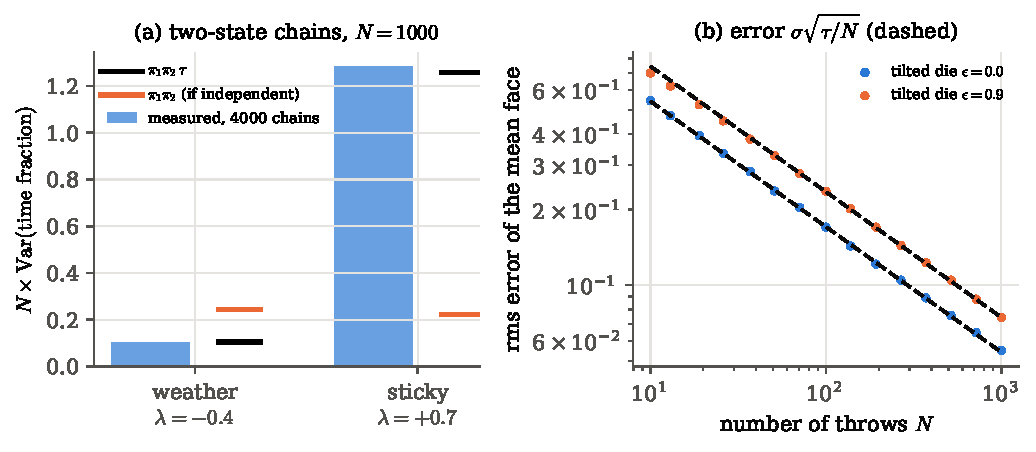
\includegraphics[width=\linewidth]{figures/ch09/ergodic_average.pdf}
\caption{The cost (or benefit) of correlated steps. (a) $N$ times the variance of the fraction
of time spent in state 1, measured over 4000 chains of 1000 steps (bars), against
$\pi_1\pi_2\tau$ (black ticks) and the value for independent draws (orange ticks). The
anticorrelated weather chain beats independent sampling; the sticky chain is almost six times
worse. (b) The rms error of the average face of the tilted die after $N$ throws, for a fair die
($\eps=0$) and a strongly tilted one ($\eps=0.9$); both follow $\sigma\sqrt{\tau/N}$ (dashed).}
\label{9a:fig:ergodic}
\end{figure}

\paragraph{One long history.}
\Cref{9a:fig:running} follows the fraction of rainy days along a single weather history of
$\NineAErgLong$ days that starts on a rainy day. The early fraction is dominated by the start and
by chance; after a few hundred days it lives inside the band $\pi_R\pm2\sqrt{\pi_R(1-\pi_R)\tau/N}$,
with $\tau=\NineAErgRainTau$ for the rain indicator, and at the end it is $\NineAErgRainFrac$,
against $\tfrac16=0.1667$, with a predicted standard error of $\NineAErgRainErr$. The starting
point has been forgotten twice over: its influence on the distribution decays as $0.6^t$, and its
weight in the running average is diluted as $1/N$.

\begin{figure}[htbp]
\centering
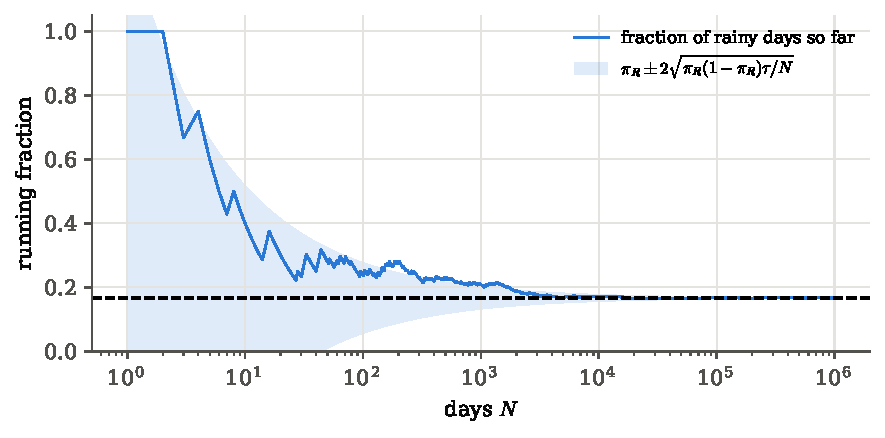
\includegraphics[width=0.8\linewidth]{figures/ch09/ergodic_running.pdf}
\caption{The fraction of rainy days so far along one simulated weather history, started on a
rainy day, on a logarithmic time axis. It settles on $\pi_R=\frac16$ (dashed) and stays within
the two-standard-error band predicted by \eqref{9a:eq:var-time-average}.}
\label{9a:fig:running}
\end{figure}

\paragraph{How much the start biases a finite run.}
Started out of equilibrium, from a distribution $p_0$, the chain's expected value of $g$ at
step $t$ is $p_tg=\sum_jp_t(j)g(j)$. By the spectral expansion \eqref{9a:eq:spectral},
$p_t=\pi+\sum_{k\ge2}c_k\lambda_k^t\ell_k$, with $c_k$ the weights of the starting distribution
along the left eigenvectors $\ell_k$, so
\begin{equation*}
  \E g(X_t)-\E_\pi g=\sum_{k\ge2}c_k\,\lambda_k^t\,(\ell_kg)\simeq c\,\lambda_2^t,
  \qquad c\equiv c_2\,(\ell_2g),
\end{equation*}
where at late times the slowest mode dominates. The amplitude $c$ is the product of how far the
start sits along the slowest mode ($c_2$) and how strongly $g$ responds to that mode ($\ell_2g$).
(For a reversible chain $\lambda_2$ is real, \cref{9a:sec:detailed-balance}.) Averaging over the
$N$ steps of the run,
\begin{align}
  \E(\bar g_N)-\E_\pi g
  &\eqby{1}\frac1N\sum_{t=1}^N\bigl(\E g(X_t)-\E_\pi g\bigr)
   \eqby{2}\frac cN\sum_{t=1}^N\lambda_2^t
   \eqby{3}\frac cN\sum_{t=1}^\infty\lambda_2^t
   \eqby{4}\frac{c\,\lambda_2}{N(1-\lambda_2)} .
  \label{9a:eq:burnin-bias}
\end{align}
\begin{explain}
  \item The mean of an average is the average of the means.
  \item The transient of each step, keeping the slowest mode.
  \item The terms beyond $t=N$ add $\lambda_2^{N+1}/(1-\lambda_2)$, negligible once
        $N$ is many relaxation times.
  \item Geometric series, $\sum_{t\ge1}\lambda^t=\lambda/(1-\lambda)$ for $\abs\lambda<1$.
\end{explain}
The start causes a bias of order $1/N$, while the statistical error $\sigma\sqrt{\tau/N}$ of
\eqref{9a:eq:var-time-average} is of order $1/\sqrt N$. For a long chain the start is harmless:
the bias shrinks faster than the noise. For a short chain started far from the bulk of $\pi$,
where $c$ is large and $\lambda_2$ close to 1, it is not, and practitioners discard the first
part of the chain, the \newterm{burn-in}.

\paragraph{The conventions of a CMB analysis.}
Dunkley et al.\ asked a practical question \cite{Dunkley2005}: how long must a chain for
cosmological parameters be, and how much of its start must be thrown away, before the table of
means and errors it produces stops changing when the chain is run longer? Their answers are two
rules of thumb, and both follow from the formulas above.

\emph{Stop when the chain mean is good to a tenth of an error bar.} They ask for the variance of
the chain mean to be below one percent of the posterior variance. Their convergence ratio $r$,
the variance of the chain mean divided by the variance of the parameter, is in our symbols
$\Var(\bar g_N)/\sigma^2=\tau/N$ by \eqref{9a:eq:var-time-average}, with $g$ the parameter. So
\begin{equation*}
  \frac{\sigma^2\tau}{N}\le0.01\,\sigma^2
  \quad\Longleftrightarrow\quad
  \frac N\tau\ge100:
\end{equation*}
at least about $100$ effective samples per parameter, and then the Monte Carlo error of a posterior
mean is a tenth of its posterior error bar. Their chain length is our $N$, and their correlation
length plays the role of our $\tau$.

\emph{Discard until the density is within a factor 10 of its peak.} Their burn-in rule removes
the start of the chain until the target density has risen to a tenth of its maximum. For a
Gaussian posterior in one parameter the density relative to the peak is $e^{-z^2/2}$ at $z$
standard deviations, so
\begin{equation*}
  e^{-z^2/2}=0.1\quad\Longleftrightarrow\quad z=\sqrt{2\ln10}\approx2.15 .
\end{equation*}
A walker that has reached that level is within about two standard deviations of the peak, in the
bulk of the posterior, where $c$ in \eqref{9a:eq:burnin-bias} is no longer large. In $d$
parameters the same rule means $\Delta\chi^2=2\ln10\approx4.6$ from the best fit, and since
typical posterior points sit at $\Delta\chi^2\approx d$, for a handful of parameters this is
already among typical points.

The toy chains of this section check the ingredients of both rules, $\tau$ and the $\lambda_2^t$
transient, against exact values; a CMB chain has to estimate them from its own output.

\begin{inpractice}[Chain averages as posterior summaries]
Every number in a cosmological parameter table produced by MCMC (CosmoMC, Cobaya, MontePython,
\texttt{emcee}) is a time average \eqref{9a:eq:ergodic} along a few long chains: a posterior mean is
the chain mean of $\theta$, a credible interval is a pair of chain quantiles, a marginal is the
histogram of one column. Its Monte Carlo error is $\sigma\sqrt{\tau/N}$, and the stopping rule
$N/\tau\gtrsim100$ effective samples per parameter derived above keeps it at a tenth of the
posterior error. In the toy chains
above, the Monte Carlo \emph{verifies} formulas we derived ($\tau$, Kac, $\abs{\lambda_2}^t$); in a
real analysis $\tau$ and $\lambda_2$ are unknown and must be estimated from the chain itself. Scale
is the other difference. Our chains have $10^3$--$10^6$ steps of a model that costs nanoseconds,
and run in seconds on a laptop; a Planck analysis runs 4--8 chains of $10^5$--$10^6$ steps with a
Boltzmann code costing about a second per step, which takes days on a cluster. A laptop-scale CMB
analysis keeps the run short by replacing the Boltzmann code with an emulated or
Taylor-expanded spectrum, at the price of a restricted parameter range and some loss of
accuracy.
\end{inpractice}
\section{The walker that never settles: free diffusion}
\label{9a:sec:diffusion}

Take Kruschke's politician of \cref{9a:sec:markov} and remove two things: the ends of the
archipelago and his habit of comparing populations. He now lives on an endless chain of
islands, flips a coin every morning, and moves to the left or right neighbour as the coin says,
whatever the islands look like. Make the islands into a continuous coastline and the coin into
a Gaussian, and this is the simplest continuous Markov chain there is: the \newterm{unbiased
random walk}
\begin{equation}
  X_{t+1}=X_t+s\,Z_{t+1},\qquad Z_1,Z_2,\dots\ \text{iid}\ \Normal(0,1),
  \label{9a:eq:free-walk}
\end{equation}
where $s$ is the step size and each $Z_t$ is a fresh standard Gaussian draw. Its transition kernel
(\cref{9a:sec:kernel}, the density of the next position $y$ given the current position $x$) is
$p(x,y)=\varphi_s(y-x)$, with $\varphi_s$ the $\Normal(0,s^2)$ density. It is what a Markov chain
sampler does if we keep its proposals and throw away every rule that refers to the target. It is
also a Brownian particle observed once per time step.

Every result of the previous sections needed some pull towards a target distribution $\pi$:
the politician's acceptance rule, the weather's fixed transition probabilities on a finite set
of states. Here there is none, and the walker is free to wander over the whole real line.

\paragraph{The questions.}
\begin{enumerate}[itemsep=1pt]
  \item Where is the walker after $t$ steps, and does the histogram of many walkers settle down?
  \item Is there a stationary density, one that the walk would leave unchanged?
  \item Does the walk at least forget its starting point?
\end{enumerate}

\subsection{Where the walker is after $t$ steps}
\label{9a:sec:free-spread}

Unrolling \eqref{9a:eq:free-walk} from a fixed start $X_0=x_0$ gives the position as the start
plus a sum of independent kicks:
\begin{align}
  X_t
  &\eqby{1}x_0+s\,(Z_1+Z_2+\dots+Z_t),
  \nonumber\\
  \E X_t&\eqby{2}x_0,
  \qquad
  \Var X_t\eqby{3}s^2\bigl(\Var Z_1+\dots+\Var Z_t\bigr)=s^2t,
  \nonumber\\
  X_t&\;\sim\;\Normal\bigl(x_0,\,s^2t\bigr).
  \label{9a:eq:free-spread}
\end{align}
\begin{explain}
  \item Apply \eqref{9a:eq:free-walk} $t$ times: $X_t=X_{t-1}+sZ_t=X_{t-2}+sZ_{t-1}+sZ_t=\dots$
  \item Each $Z_k$ has mean zero.
  \item The kicks are independent, so their variances add (\cref{ch:01}); each $Z_k$ has
        variance 1.
\end{explain}
The last line holds because a sum of independent Gaussians is Gaussian (\cref{ch:02}). The
centre never moves, because the walk is unbiased; the width grows as $s\sqrt t$, without limit.
This is the random-walk law of Brownian motion, $\langle(X_t-x_0)^2\rangle\propto t$, which
Einstein used to connect the jiggling of pollen grains to the size of molecules.

The same result can be read as an equation for the density of walkers. One step convolves the
density with the kernel, $f_{t+1}(y)=\int f_t(x)\,\varphi_s(y-x)\,\dd x$
(\cref{9a:eq:kernel-evolve}). Substitute $x=y-u$ and expand $f_t$ around $y$ for small steps:
\begin{align}
  f_{t+1}(y)
  &\eqby{1}\int f_t(y-u)\,\varphi_s(u)\,\dd u
  \nonumber\\
  &\eqby{2}\int\Bigl[f_t(y)-u\,f_t'(y)+\tfrac12u^2f_t''(y)-\dots\Bigr]\varphi_s(u)\,\dd u
  \nonumber\\
  &\eqby{3}f_t(y)+\tfrac12s^2f_t''(y)+O\bigl(s^4f_t''''\bigr).
  \label{9a:eq:diffusion-step}
\end{align}
\begin{explain}
  \item Change of variable $u=y-x$; $\varphi_s$ is even, so $\varphi_s(y-x)=\varphi_s(u)$.
  \item Taylor expansion of $f_t$ about $y$, valid when $f_t$ varies little over one step $s$.
  \item The kernel integrates to 1, has mean $\int u\,\varphi_s\,\dd u=0$ and variance
        $\int u^2\varphi_s\,\dd u=s^2$; the next surviving term is the fourth moment, $3s^4$.
\end{explain}
\emph{From steps to a clock.} Suppose the walker takes one step every $\Delta t$ seconds. Call
the step number $n$ (it was $t$ in \eqref{9a:eq:diffusion-step}), so that after $n$ steps the
physical time is $t=n\,\Delta t$, and write $f(x,t)$ for the density of walkers at that time.
For small steps taken often, the density changes little from one step to the next, and
\begin{align*}
  \Delta t\,\frac{\partial f}{\partial t}
  &\eqby{1}f(x,t+\Delta t)-f(x,t)
   \eqby{2}f_{n+1}(x)-f_n(x)
   \eqby{3}\tfrac12s^2\,\frac{\partial^2f}{\partial x^2}.
\end{align*}
\begin{explain}
  \item The first-order Taylor expansion in time, valid when $f$ changes little during one
        step.
  \item One step of the clock is one step of the walk.
  \item \eqref{9a:eq:diffusion-step}, dropping the higher-order term.
\end{explain}
Dividing by $\Delta t$ gives the \newterm{diffusion equation}
\begin{equation}
  \frac{\partial f}{\partial t}=D\,\frac{\partial^2f}{\partial x^2},
  \qquad D=\frac{s^2}{2\,\Delta t},
  \label{9a:eq:diffusion}
\end{equation}
the heat equation, with the \newterm{diffusion coefficient} $D$ collecting the step size and the
step rate. Its solution from a point is the spreading Gaussian of \eqref{9a:eq:free-spread}, and
the two descriptions agree on the width: after $n=t/\Delta t$ steps the variance is
$s^2n=s^2t/\Delta t=2Dt$. A density of
walkers behaves exactly like a drop of ink in still water.

\paragraph{Example: twenty thousand walkers.}
\Cref{9a:fig:diffusion} follows $\NineADiffWalkers$ independent walkers with $s=1$, all started at
the origin. The histograms at $t=10$, $100$, $1000$ lie on the Gaussians
$\Normal(0,t)$, and the sample variance is $\NineADiffVarHundred$ at $t=100$ and
$\NineADiffVarThousand$ at $t=1000$, against $s^2t=100$ and $1000$. The core of the simulation is
eight lines:

\pyfile[firstline=20,lastline=27,firstnumber=20]{code/ch09/07_random_walk_diffusion.py}{The unbiased random walk for many walkers at once}
Line 20 puts every walker at the origin. Line 23 is \eqref{9a:eq:free-walk} applied to all of them
in one vectorised step: each walker gets its own fresh Gaussian kick. Line 24 records the spread of
the crowd, and lines 25--26 keep three snapshots for the histograms. Nothing in the loop refers to
any target; the walkers obey the kernel and nothing else.

\begin{figure}[htbp]
\centering
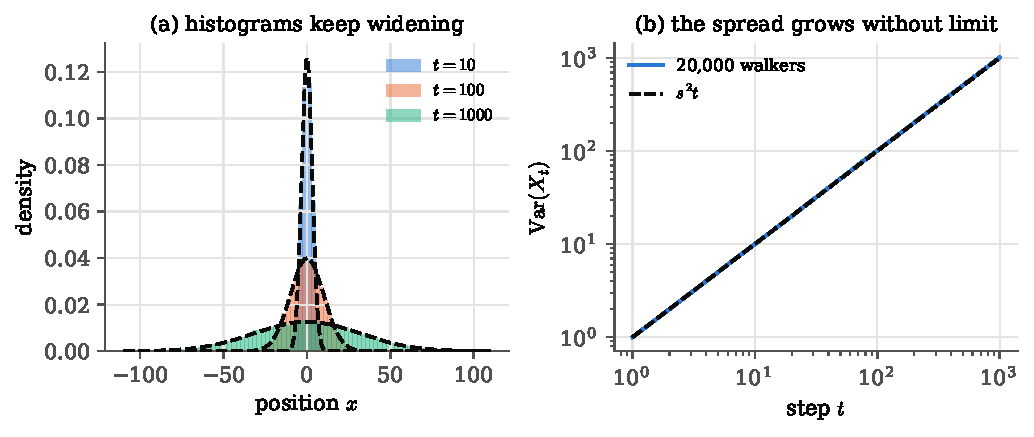
\includegraphics[width=\linewidth]{figures/ch09/random_walk_diffusion.pdf}
\caption{The unbiased walker never settles. (a) Histograms of $20\,000$ walkers started at the
origin, after 10, 100 and 1000 steps of size $s=1$, with the Gaussians $\Normal(0,s^2t)$
(dashed): the crowd keeps flattening. (b) The variance of the crowd grows in proportion to the
number of steps, on a log--log scale, with no sign of levelling off.}
\label{9a:fig:diffusion}
\end{figure}

\subsection{No stationary density}
\label{9a:sec:no-stationary}

The histograms flatten for ever, which suggests that there is nothing for them to converge to.
Let us prove it. A stationary density $f$ would satisfy $f=f*\varphi_s$, a convolution. The
convolution theorem turns this into a product for the characteristic functions
$\chi_f(k)=\E\,e^{ikX}=\int f(x)e^{ikx}\,\dd x$, the Fourier transforms of the densities, and the
characteristic function of the Gaussian kick is $e^{-s^2k^2/2}$ (\cref{ch:02}). So
\begin{align}
  \chi_f(k)
  &\eqby{1}\chi_f(k)\,e^{-s^2k^2/2}
  \quad\Longrightarrow\quad
  \chi_f(k)\bigl(1-e^{-s^2k^2/2}\bigr)\eqby{2}0
  \quad\Longrightarrow\quad
  \chi_f(k)\eqby{3}0\ \ \text{for every }k\ne0 .
  \label{9a:eq:no-stationary}
\end{align}
\begin{explain}
  \item $X_{t+1}=X_t+sZ$ with $X_t\sim f$ independent of $Z$, so
        $\E e^{ikX_{t+1}}=\E e^{ikX_t}\,\E e^{iksZ}$, and stationarity demands $X_{t+1}\sim f$.
  \item Move everything to one side.
  \item The bracket is nonzero for $k\ne0$.
\end{explain}
But every probability density has $\chi_f(0)=\int f=1$ and a characteristic function that is
continuous in $k$. One that is zero for every $k\ne0$ cannot jump to 1 at $k=0$. So no
probability density is stationary for the free walk.

Detailed balance points to the same answer from another side. The kernel is symmetric,
$p(x,y)=\varphi_s(y-x)=p(y,x)$, so the detailed-balance condition
$f(x)p(x,y)=f(y)p(y,x)$ of \cref{9a:sec:kernel} reduces to $f(x)=f(y)$: the only balanced
``distribution'' is a constant, the flat measure over the whole line. It cannot be normalised.
The unbiased walker is, in this precise sense, trying to sample a uniform distribution on
$\mathbb R$, and there is no such distribution. In the language of \cref{9a:sec:recurrence}, the
one-dimensional walk is null recurrent: it returns to every neighbourhood, but only after
excursions so long that the mean return time $m$ is infinite, and Kac's formula
\eqref{9a:eq:kac}, $\pi=1/m$, assigns every region probability zero.

\subsection{Forgetting without settling}
\label{9a:sec:forget-no-settle}

The third question is subtler. Start one crowd at $x_0=0$ and another at $x_0=a$. After $t$
steps they are $\Normal(0,\sigma_t^2)$ and $\Normal(a,\sigma_t^2)$ with $\sigma_t=s\sqrt t$. How
different are they? For two Gaussians of equal width the densities cross at the midpoint $a/2$,
so the event on which the first exceeds the second is $\{x<a/2\}$, and the total-variation
distance \eqref{9a:eq:tv} (written for densities, $\tfrac12\int\abs{p-q}\,\dd x$) is
\begin{align}
  \norm{\Normal(0,\sigma_t^2)-\Normal(a,\sigma_t^2)}_{\rm TV}
  &\eqby{1}\Prob_0\Bigl(X<\frac a2\Bigr)-\Prob_a\Bigl(X<\frac a2\Bigr)
  \eqby{2}\Phi\Bigl(\frac a{2\sigma_t}\Bigr)-\Phi\Bigl(-\frac a{2\sigma_t}\Bigr)
  \nonumber\\
  &\eqby{3}2\,\Phi\Bigl(\frac a{2\sigma_t}\Bigr)-1
  \;\simeq\;\frac{a}{\sigma_t\sqrt{2\pi}}
  =\frac{a}{s\sqrt{2\pi t}} .
  \label{9a:eq:tv-gauss-shift}
\end{align}
\begin{explain}
  \item The maximum of $\abs{p(A)-q(A)}$ is reached on the set where $p>q$
        (\cref{9a:sec:convergence}), here $\{x<a/2\}$.
  \item Standardise: under $\Normal(\mu,\sigma^2)$, $\Prob(X<c)=\Phi\bigl((c-\mu)/\sigma\bigr)$,
        with $\Phi$ the standard normal CDF.
  \item $\Phi(-z)=1-\Phi(z)$; then for small $z$, $\Phi(z)\simeq\tfrac12+z/\sqrt{2\pi}$, since the
        standard normal density at 0 is $1/\sqrt{2\pi}$.
\end{explain}
The distance goes to zero: the walk does forget where it started. Two crowds launched from
different islands become indistinguishable, because both spread so widely that the initial
offset is a negligible fraction of their width. But the forgetting is slow, like $1/\sqrt t$ rather
than geometrically, and, more importantly, the two crowds do not converge to anything. They just
become equally flat.

\begin{pitfall}[Forgetting the start is not converging]
A chain can lose all memory of its initial distribution and still have no equilibrium to offer.
The free walk does exactly that. For a sampler both properties are needed: a normalisable
stationary distribution $\pi$ (for a countable chain, positive recurrence) and convergence to it.
Time averages along a free walk do not estimate anything: the fraction of time spent in any
bounded interval goes to zero.
\end{pitfall}

\subsection{The walker with a pull}
\label{9a:sec:ar1-forgetting}

Add a restoring pull to the free walk and everything comes back. The AR(1) chain of
\cref{9a:sec:kernel} keeps only a fraction $\rho$ of the current position before the kick,
\begin{equation}
  X_{t+1}=\rho\,X_t+\sqrt{1-\rho^2}\;Z_{t+1},\qquad \abs\rho<1,
  \label{9a:eq:ar1}
\end{equation}
which is a Brownian particle in a harmonic well, observed at discrete times; we showed there that
it satisfies detailed balance with respect to $\Normal(0,1)$. Unrolling it from $X_0=x_0$, the
same way as \eqref{9a:eq:free-spread},
\begin{align}
  X_t
  &\eqby{1}\rho^t x_0+\sqrt{1-\rho^2}\sum_{k=0}^{t-1}\rho^k Z_{t-k},
  \nonumber\\
  \E X_t&\eqby{2}\rho^t x_0,
  \qquad
  \Var X_t\eqby{3}(1-\rho^2)\sum_{k=0}^{t-1}\rho^{2k}\eqby{4}1-\rho^{2t}.
  \label{9a:eq:ar1-unroll}
\end{align}
\begin{explain}
  \item Substitute \eqref{9a:eq:ar1} into itself $t$ times: the start is multiplied by $\rho$ at
        every step, and the kick received $k$ steps ago by $\rho^k$.
  \item The kicks have mean zero.
  \item Independent kicks, each of variance 1, multiplied by $\sqrt{1-\rho^2}\,\rho^k$.
  \item Geometric sum, $\sum_{k=0}^{t-1}\rho^{2k}=(1-\rho^{2t})/(1-\rho^2)$.
\end{explain}
So $X_t\sim\Normal(\rho^tx_0,\,1-\rho^{2t})\to\Normal(0,1)$ for every start. Compare with the free
walk: the width now saturates at 1, and the offset of the start shrinks as $\rho^t$. Two crowds
started at $x_0$ and $x_0'$ have the same width $\sqrt{1-\rho^{2t}}$ and centres $\rho^tx_0$ and
$\rho^tx_0'$, so \eqref{9a:eq:tv-gauss-shift} with offset $a=\rho^t\abs{x_0-x_0'}$ gives a
distance $\simeq\rho^t\abs{x_0-x_0'}/\sqrt{2\pi}$ once $\rho^{2t}\ll1$: geometric forgetting at
rate $\rho$.

The rate $\rho$ plays the part of $\lambda_2$ of \cref{9a:sec:eigen}. For a finite chain $\lambda_2$
belonged to a right eigenvector $v$, with $(Pv)_i=\E\bigl(v(X_1)\given X_0=i\bigr)=\lambda_2v_i$.
The continuous analogue is a function $g$ whose conditional expectation one step later is a
multiple of itself:
\begin{align}
  \E\bigl(X_{1}\given X_0=x\bigr)
  &\eqby{1}\rho\,x,
  \nonumber\\
  \E\bigl(X_{1}^2-1\given X_0=x\bigr)
  &\eqby{2}\rho^2x^2+(1-\rho^2)-1
  =\rho^2\,(x^2-1),
  \nonumber\\
  \E\bigl(X_{1}^3-3X_1\given X_0=x\bigr)
  &\eqby{3}\rho^3x^3+3\rho x(1-\rho^2)-3\rho x
  =\rho^3\,(x^3-3x).
  \label{9a:eq:ar1-eigen}
\end{align}
\begin{explain}
  \item The kick has mean zero.
  \item $\E\bigl((\rho x+\sqrt{1-\rho^2}Z)^2\bigr)=\rho^2x^2+2\rho x\sqrt{1-\rho^2}\,\E Z
        +(1-\rho^2)\E Z^2$, with $\E Z=0$ and $\E Z^2=1$.
  \item Write $\sigma=\sqrt{1-\rho^2}$ and expand the cube:
        $(\rho x+\sigma Z)^3=\rho^3x^3+3\rho^2x^2\sigma Z+3\rho x\sigma^2Z^2+\sigma^3Z^3$, with
        $\E Z=\E Z^3=0$ (the Gaussian is symmetric) and $\E Z^2=1$; the $-3X_1$ term has
        expectation $-3\rho x$. The terms in $x$ then combine to $3\rho x(1-\rho^2-1)=-3\rho^3x$.
\end{explain}
So $g_1(x)=x$ is an eigenfunction with eigenvalue $\rho$, $g_2(x)=x^2-1$ one with eigenvalue
$\rho^2$, and $g_3(x)=x^3-3x$ one with eigenvalue $\rho^3$. Each is the power $x^n$ minus
lower powers chosen to cancel the extra terms the kick produces. These are the Hermite polynomials, and the
pattern continues: the $n$th Hermite polynomial has eigenvalue $\rho^n$ (Mehler's formula, not
proved here). The slowest non-trivial mode decays as $\rho^t$, exactly the rate found for the
mean in \eqref{9a:eq:ar1-unroll}. The variance lives in the $x^2-1$ mode: by
\eqref{9a:eq:ar1-unroll} its distance from the target value 1 is $1-\Var X_t=\rho^{2t}=(\rho^2)^t$,
the eigenvalue $\rho^2$ of that mode raised to the power $t$, so it relaxes twice as fast in the
exponent.

\paragraph{Example: three starts, one law.}
With $\rho=0.9$, \cref{9a:fig:ar1} starts three crowds of $\NineADiffWalkers$ walkers at
$x_0=-20$, $0$ and $+20$, twenty standard deviations of the target apart. The means follow
$\rho^tx_0$: from $x_0=20$ the crowd's mean after 40 steps is $\NineAARMeanForty$, against
$20\times0.9^{40}=\NineAARMeanFortyPred$. After 80 steps the three histograms lie on top of
$\Normal(0,1)$; the crowd started at $+20$ has mean $\NineAARMeanEnd$ and variance
$\NineAARVarEnd$, against $0$ and $1-0.9^{160}\simeq\NineAARVarEndPred$. Everything a sampler needs
is present: a normalisable stationary law, and geometric forgetting of the start.

\begin{figure}[htbp]
\centering
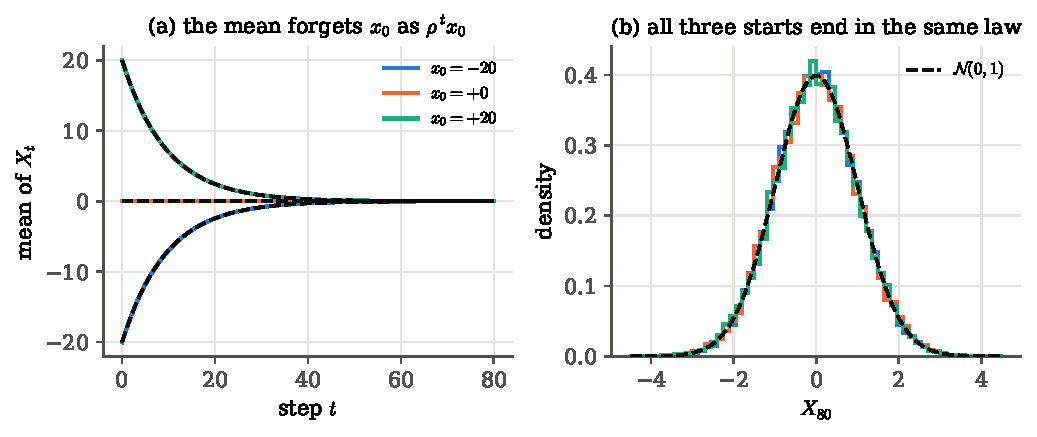
\includegraphics[width=\linewidth]{figures/ch09/ar1_forgetting.pdf}
\caption{The walker with a pull, $X_{t+1}=0.9X_t+\sqrt{1-0.81}\,Z$, forgets where it started.
(a) The mean position of three crowds started at $-20$, $0$ and $+20$ (solid) follows
$\rho^tx_0$ (dashed) back to zero. (b) After 80 steps the three crowds have the same histogram,
the standard Gaussian (dashed).}
\label{9a:fig:ar1}
\end{figure}

\paragraph{Example: the free walk on a ring.}
Is it the randomness or the endless line that stops the free walker from settling? Wrap the line
into a ring of $K$ islands, and let the walker stay put with probability $\tfrac12$ and step to
each neighbour with probability $\tfrac14$ (staying put removes the period 2 of
\cref{9a:sec:period}). There is still no bias anywhere. The rows of the transition matrix sum to
one and so do its columns (each island receives $\tfrac12$ from itself and $\tfrac14$ from each
neighbour), so the uniform distribution $\pi_j=1/K$ is stationary:
$\sum_i\pi_ip_{ij}=\tfrac1K\sum_ip_{ij}=\tfrac1K\cdot1$. The
eigenvectors are the Fourier modes $v_j=e^{2\pi i\,jk/K}$, $k=0,\dots,K-1$, the normal modes of a
ring of coupled oscillators:
\begin{align}
  (Pv)_j
  &\eqby{1}\tfrac12v_j+\tfrac14v_{j+1}+\tfrac14v_{j-1}
  \eqby{2}v_j\Bigl[\tfrac12+\tfrac14\bigl(e^{2\pi ik/K}+e^{-2\pi ik/K}\bigr)\Bigr]
  \nonumber\\
  &\eqby{3}v_j\,\frac{1+\cos(2\pi k/K)}{2}
  \eqby{4}v_j\cos^2\frac{\pi k}{K}.
  \label{9a:eq:ring}
\end{align}
\begin{explain}
  \item One step: stay with probability $\tfrac12$, move to either neighbour with $\tfrac14$
        (indices modulo $K$, which is the ring).
  \item $v_{j\pm1}=v_j\,e^{\pm2\pi ik/K}$.
  \item $e^{i\phi}+e^{-i\phi}=2\cos\phi$.
  \item $1+\cos2\alpha=2\cos^2\alpha$.
\end{explain}
\emph{Which mode is slowest?} The eigenvalue $\cos^2(\pi k/K)$ lies between 0 and 1, and it is
largest when the angle $\pi k/K$ is closest to $0$ or to $\pi$. The mode $k=0$ gives exactly 1:
it is the constant vector, the uniform distribution itself. Among the others, the angle is
closest to $0$ or $\pi$ for $k=1$ and $k=K-1$, the longest waves round the ring, so
$\lambda_2=\cos^2(\pi/K)$ (shared by the two). The distance from uniform decays as
$\cos^{2t}(\pi/K)$, and the relaxation time is
\begin{equation*}
  \frac1{1-\lambda_2}=\frac1{\sin^2(\pi/K)}\simeq\frac{K^2}{\pi^2}\ \text{steps},
\end{equation*}
using $1-\cos^2=\sin^2$ and, for large $K$, $\sin x\simeq x$ for the small angle $x=\pi/K$. For
$K=10$ islands, $\sin18^\circ=0.309$, $\sin^218^\circ=0.0955$, and $1/0.0955\simeq10.5$
steps; for $K=100$, $1/\sin^21.8^\circ\simeq1013$, against $K^2/\pi^2=1013$. On a finite ring the free
walker does settle, and its target is the flat distribution it was ``trying'' to sample all along.
But the time it takes grows as the \emph{square} of the size of the space, the signature of
diffusion: to cross $K$ sites with steps of size one takes about $K^2$ steps.

\paragraph{What diffusion costs a sampler.}
The ring makes a point that every random-walk sampler pays for. A chain that explores by
unbiased local steps of size $s$ needs about $(L/s)^2$ steps to cross a region of size $L$. Large
steps would cross faster, but on a peaked target most of them land where the probability is tiny.
The politician's acceptance rule of \cref{9a:sec:markov} and the Metropolis--Hastings rule built
from detailed balance keep the unbiased proposal of \eqref{9a:eq:free-walk} and add exactly the
bias that is missing here, turning the unbiased walker into the biased one of
\cref{9a:sec:oscillator}: a step towards higher probability is always taken, a step away from it
only sometimes, so that the walker lingers where the target is large
\srcref{Kruschke}{§7.2.1}, \mainref{p.~411}. The diffusive cost then sets the length of every
MCMC run. In the laptop examples of this chapter it means $10^4$--$10^5$ steps of a fast model; a
full cosmological analysis, with a dozen correlated parameters and an expensive likelihood, needs
the same order of steps per chain but at a second per step, which is why it runs on a cluster.

\begin{recap}
\begin{itemize}
  \item A sample is the distribution for every practical purpose. An oscillator of fixed energy
        samples its own orbit when looked at at random instants, because its motion covers the
        orbit at the right rate; time average equals ensemble average. Many coupled degrees of
        freedom, a canonical ensemble or a posterior offer no such motion, so we build one.
  \item A Markov chain remembers one step: the next state depends only on the current one,
        through a transition matrix $P$ (rows are pmfs) or kernel $p(x,y)$. A distribution of
        walkers evolves as $p_{t+1}=p_tP$, and $P^n$ gives the $n$-step probabilities
        (Chapman--Kolmogorov). The MLE of $p_{ij}$ from one history is $n_{ij}/n_i$.
  \item States split into communicating classes. A good sampler is irreducible (every state
        reachable from every other), positive recurrent (finite mean return time) and aperiodic.
        The symmetric walk on the integers is recurrent but null; biased, it is transient.
  \item $\pi$ is stationary if $\pi P=\pi$: probability flowing in balances probability flowing out.
        Detailed balance, $\pi_ip_{ij}=\pi_jp_{ji}$, is a sufficient condition with no net
        current between any pair, the analogue of thermodynamic equilibrium; a circulating
        current can be stationary without it.
  \item A finite irreducible aperiodic chain forgets its starting distribution geometrically:
        $\norm{p_t-\pi}_{\rm TV}\simeq C\abs{\lambda_2}^t$, and the Doeblin contraction bounds it by
        $(1-\delta)^t$; coupling gives the same result by letting two walkers meet.
  \item The ergodic theorem: time averages along one walk converge to averages over $\pi$, also
        for periodic chains. Their variance is $\sigma^2\tau/N$ with
        $\tau=1+2\sum_k\rho_k$, so $N$ steps are worth $N/\tau$ independent draws; and
        $\pi_j=1/m_j$ (Kac).
  \item The unbiased random walk on the line spreads as $s\sqrt t$, obeys the diffusion equation,
        and has no normalisable stationary density: it forgets its start, like $1/\sqrt t$, but
        has nothing to converge to. A restoring pull (AR(1)) gives a stationary $\Normal(0,1)$
        and forgetting at rate $\rho^t$. The missing bias is what Metropolis--Hastings supplies.
\end{itemize}
\end{recap}
\providecommand{\NineBBwN}{}\renewcommand{\NineBBwN}{50\,000}
\providecommand{\NineBBwStep}{}\renewcommand{\NineBBwStep}{1.5}
\providecommand{\NineBBwAccDrunk}{}\renewcommand{\NineBBwAccDrunk}{1}
\providecommand{\NineBBwAccMetro}{}\renewcommand{\NineBBwAccMetro}{0.5426}
\providecommand{\NineBBwAccClimb}{}\renewcommand{\NineBBwAccClimb}{2.200\times10^{-4}}
\providecommand{\NineBBwDrunkEnd}{}\renewcommand{\NineBBwDrunkEnd}{-38.75}
\providecommand{\NineBBwDrunkScale}{}\renewcommand{\NineBBwDrunkScale}{335.4}
\providecommand{\NineBBwClimbEnd}{}\renewcommand{\NineBBwClimbEnd}{2.000}
\providecommand{\NineBBwFracRight}{}\renewcommand{\NineBBwFracRight}{0.7083}
\providecommand{\NineBBwMean}{}\renewcommand{\NineBBwMean}{0.8518}
\providecommand{\NineBBwMeanExact}{}\renewcommand{\NineBBwMeanExact}{0.8}
\providecommand{\NineBBwVar}{}\renewcommand{\NineBBwVar}{3.84}
\providecommand{\NineBBwVarExact}{}\renewcommand{\NineBBwVarExact}{3.916}
\providecommand{\NineBBwRightLow}{}\renewcommand{\NineBBwRightLow}{0.5929}
\providecommand{\NineBBwRightExactLow}{}\renewcommand{\NineBBwRightExactLow}{0.5915}
\providecommand{\NineBBwRightOne}{}\renewcommand{\NineBBwRightOne}{0.6937}
\providecommand{\NineBBwRightExactOne}{}\renewcommand{\NineBBwRightExactOne}{0.6957}
\providecommand{\NineBBwRightThree}{}\renewcommand{\NineBBwRightThree}{0.8742}
\providecommand{\NineBBwRightExactThree}{}\renewcommand{\NineBBwRightExactThree}{0.8772}
\providecommand{\NineBHbN}{}\renewcommand{\NineBHbN}{200\,000}
\providecommand{\NineBHbStep}{}\renewcommand{\NineBHbStep}{2}
\providecommand{\NineBHbLowExact}{}\renewcommand{\NineBHbLowExact}{0.01439}
\providecommand{\NineBHbMeanA}{}\renewcommand{\NineBHbMeanA}{3.008}
\providecommand{\NineBHbLowA}{}\renewcommand{\NineBHbLowA}{0.01464}
\providecommand{\NineBHbAccA}{}\renewcommand{\NineBHbAccA}{0.6225}
\providecommand{\NineBHbMeanB}{}\renewcommand{\NineBHbMeanB}{3.183}
\providecommand{\NineBHbLowB}{}\renewcommand{\NineBHbLowB}{0.009384}
\providecommand{\NineBHbAccB}{}\renewcommand{\NineBHbAccB}{0.7093}
\providecommand{\NineBHbMeanC}{}\renewcommand{\NineBHbMeanC}{2.975}
\providecommand{\NineBHbLowC}{}\renewcommand{\NineBHbLowC}{0.01402}
\providecommand{\NineBHbAccC}{}\renewcommand{\NineBHbAccC}{0.7086}
\providecommand{\NineBHbMeanD}{}\renewcommand{\NineBHbMeanD}{3.012}
\providecommand{\NineBHbLowD}{}\renewcommand{\NineBHbLowD}{0.01366}
\providecommand{\NineBHbAccD}{}\renewcommand{\NineBHbAccD}{0.5573}
\providecommand{\NineBHbMeanE}{}\renewcommand{\NineBHbMeanE}{1.989}
\providecommand{\NineBHbLowE}{}\renewcommand{\NineBHbLowE}{0.09093}
\providecommand{\NineBHbAccE}{}\renewcommand{\NineBHbAccE}{0.6234}
\providecommand{\NineBCauAccSmall}{}\renewcommand{\NineBCauAccSmall}{0.9731}
\providecommand{\NineBCauHalfSmall}{}\renewcommand{\NineBCauHalfSmall}{0.8332}
\providecommand{\NineBCauHalfLongSmall}{}\renewcommand{\NineBCauHalfLongSmall}{0.5517}
\providecommand{\NineBCauTauSmall}{}\renewcommand{\NineBCauTauSmall}{608}
\providecommand{\NineBCauAccOne}{}\renewcommand{\NineBCauAccOne}{0.7723}
\providecommand{\NineBCauHalfOne}{}\renewcommand{\NineBCauHalfOne}{0.2478}
\providecommand{\NineBCauHalfLongOne}{}\renewcommand{\NineBCauHalfLongOne}{0.5032}
\providecommand{\NineBCauTauOne}{}\renewcommand{\NineBCauTauOne}{23.86}
\providecommand{\NineBCauAccBig}{}\renewcommand{\NineBCauAccBig}{0.2712}
\providecommand{\NineBCauHalfBig}{}\renewcommand{\NineBCauHalfBig}{0.5455}
\providecommand{\NineBCauHalfLongBig}{}\renewcommand{\NineBCauHalfLongBig}{0.5002}
\providecommand{\NineBCauTauBig}{}\renewcommand{\NineBCauTauBig}{15.5}
\providecommand{\NineBCoinAccSmall}{}\renewcommand{\NineBCoinAccSmall}{0.9334}
\providecommand{\NineBCoinEssSmall}{}\renewcommand{\NineBCoinEssSmall}{463}
\providecommand{\NineBCoinKrAccSmall}{}\renewcommand{\NineBCoinKrAccSmall}{0.936}
\providecommand{\NineBCoinKrEssSmall}{}\renewcommand{\NineBCoinKrEssSmall}{469}
\providecommand{\NineBCoinMeanSmall}{}\renewcommand{\NineBCoinMeanSmall}{0.6867}
\providecommand{\NineBCoinAccMid}{}\renewcommand{\NineBCoinAccMid}{0.4958}
\providecommand{\NineBCoinEssMid}{}\renewcommand{\NineBCoinEssMid}{11181}
\providecommand{\NineBCoinKrAccMid}{}\renewcommand{\NineBCoinKrAccMid}{0.495}
\providecommand{\NineBCoinKrEssMid}{}\renewcommand{\NineBCoinKrEssMid}{11724}
\providecommand{\NineBCoinMeanMid}{}\renewcommand{\NineBCoinMeanMid}{0.6812}
\providecommand{\NineBCoinAccBig}{}\renewcommand{\NineBCoinAccBig}{0.06174}
\providecommand{\NineBCoinEssBig}{}\renewcommand{\NineBCoinEssBig}{2065}
\providecommand{\NineBCoinKrAccBig}{}\renewcommand{\NineBCoinKrAccBig}{0.0624}
\providecommand{\NineBCoinKrEssBig}{}\renewcommand{\NineBCoinKrEssBig}{2113}
\providecommand{\NineBCoinMeanBig}{}\renewcommand{\NineBCoinMeanBig}{0.6812}
\providecommand{\NineBCoinMeanExact}{}\renewcommand{\NineBCoinMeanExact}{0.6818}
\providecommand{\NineBCoinLo}{}\renewcommand{\NineBCoinLo}{0.4758}
\providecommand{\NineBCoinHi}{}\renewcommand{\NineBCoinHi}{0.8547}
\providecommand{\NineBCoinLoExact}{}\renewcommand{\NineBCoinLoExact}{0.4782}
\providecommand{\NineBCoinHiExact}{}\renewcommand{\NineBCoinHiExact}{0.8541}
\providecommand{\NineBStLopt}{}\renewcommand{\NineBStLopt}{2.381}
\providecommand{\NineBStAopt}{}\renewcommand{\NineBStAopt}{0.2338}
\providecommand{\NineBStBestAccOne}{}\renewcommand{\NineBStBestAccOne}{0.4583}
\providecommand{\NineBStBestLOne}{}\renewcommand{\NineBStBestLOne}{2.26}
\providecommand{\NineBStTauDOne}{}\renewcommand{\NineBStTauDOne}{4.433}
\providecommand{\NineBStAccOptOne}{}\renewcommand{\NineBStAccOptOne}{0.4452}
\providecommand{\NineBStBestAccTen}{}\renewcommand{\NineBStBestAccTen}{0.2816}
\providecommand{\NineBStBestLTen}{}\renewcommand{\NineBStBestLTen}{2.26}
\providecommand{\NineBStTauDTen}{}\renewcommand{\NineBStTauDTen}{3.353}
\providecommand{\NineBStAccOptTen}{}\renewcommand{\NineBStAccOptTen}{0.2588}
\providecommand{\NineBStBestAccFifty}{}\renewcommand{\NineBStBestAccFifty}{0.2629}
\providecommand{\NineBStBestLFifty}{}\renewcommand{\NineBStBestLFifty}{2.26}
\providecommand{\NineBStTauDFifty}{}\renewcommand{\NineBStTauDFifty}{2.98}
\providecommand{\NineBStAccOptFifty}{}\renewcommand{\NineBStAccOptFifty}{0.2396}
\providecommand{\NineBStIsoBestTau}{}\renewcommand{\NineBStIsoBestTau}{33.67}
\providecommand{\NineBStIsoBestStep}{}\renewcommand{\NineBStIsoBestStep}{1.166}
\providecommand{\NineBStIsoBestAcc}{}\renewcommand{\NineBStIsoBestAcc}{0.2024}
\providecommand{\NineBStCorrSmallAcc}{}\renewcommand{\NineBStCorrSmallAcc}{0.9286}
\providecommand{\NineBStCorrSmallTau}{}\renewcommand{\NineBStCorrSmallTau}{2981}
\providecommand{\NineBStCorrSmallStep}{}\renewcommand{\NineBStCorrSmallStep}{0.05}
\providecommand{\NineBStCorrLargeAcc}{}\renewcommand{\NineBStCorrLargeAcc}{5.750\times10^{-4}}
\providecommand{\NineBStCorrLargeTau}{}\renewcommand{\NineBStCorrLargeTau}{1229}
\providecommand{\NineBStCorrLargeStep}{}\renewcommand{\NineBStCorrLargeStep}{30}
\providecommand{\NineBStCorrTunedAcc}{}\renewcommand{\NineBStCorrTunedAcc}{0.2009}
\providecommand{\NineBStCorrTunedTau}{}\renewcommand{\NineBStCorrTunedTau}{35.55}
\providecommand{\NineBStCorrTunedStep}{}\renewcommand{\NineBStCorrTunedStep}{1.166}
\providecommand{\NineBStCorrShapedAcc}{}\renewcommand{\NineBStCorrShapedAcc}{0.3554}
\providecommand{\NineBStCorrShapedTau}{}\renewcommand{\NineBStCorrShapedTau}{9.278}
\providecommand{\NineBStCorrShapedStep}{}\renewcommand{\NineBStCorrShapedStep}{1.683}
\providecommand{\NineBStRho}{}\renewcommand{\NineBStRho}{0.95}
\providecommand{\NineBBaSig}{}\renewcommand{\NineBBaSig}{0.3}
\providecommand{\NineBBaN}{}\renewcommand{\NineBBaN}{200\,000}
\providecommand{\NineBBaRepN}{}\renewcommand{\NineBBaRepN}{12}
\providecommand{\NineBBaRoundVarRepMean}{}\renewcommand{\NineBBaRoundVarRepMean}{2.06}
\providecommand{\NineBBaRoundVarRepSd}{}\renewcommand{\NineBBaRoundVarRepSd}{0.28}
\providecommand{\NineBBaRoundVarRepErr}{}\renewcommand{\NineBBaRoundVarRepErr}{0.08}
\providecommand{\NineBBaShapedVarRepMean}{}\renewcommand{\NineBBaShapedVarRepMean}{2.21}
\providecommand{\NineBBaShapedVarRepSd}{}\renewcommand{\NineBBaShapedVarRepSd}{0.31}
\providecommand{\NineBBaShapedVarRepErr}{}\renewcommand{\NineBBaShapedVarRepErr}{0.09}
\providecommand{\NineBBaStraightVarRepMean}{}\renewcommand{\NineBBaStraightVarRepMean}{2.07}
\providecommand{\NineBBaStraightVarRepSd}{}\renewcommand{\NineBBaStraightVarRepSd}{0.05}
\providecommand{\NineBBaStraightVarRepErr}{}\renewcommand{\NineBBaStraightVarRepErr}{0.01}
\providecommand{\NineBBaEmVarRepMean}{}\renewcommand{\NineBBaEmVarRepMean}{2.14}
\providecommand{\NineBBaEmVarRepSd}{}\renewcommand{\NineBBaEmVarRepSd}{0.20}
\providecommand{\NineBBaEmVarRepErr}{}\renewcommand{\NineBBaEmVarRepErr}{0.06}
\providecommand{\NineBBaRoundAcc}{}\renewcommand{\NineBBaRoundAcc}{0.196}
\providecommand{\NineBBaRoundTau}{}\renewcommand{\NineBBaRoundTau}{265.8}
\providecommand{\NineBBaRoundMeanTwo}{}\renewcommand{\NineBBaRoundMeanTwo}{1.025}
\providecommand{\NineBBaRoundVarTwo}{}\renewcommand{\NineBBaRoundVarTwo}{2.323}
\providecommand{\NineBBaShapedAcc}{}\renewcommand{\NineBBaShapedAcc}{0.07981}
\providecommand{\NineBBaShapedTau}{}\renewcommand{\NineBBaShapedTau}{89.19}
\providecommand{\NineBBaShapedMeanTwo}{}\renewcommand{\NineBBaShapedMeanTwo}{0.976}
\providecommand{\NineBBaShapedVarTwo}{}\renewcommand{\NineBBaShapedVarTwo}{1.887}
\providecommand{\NineBBaStraightAcc}{}\renewcommand{\NineBBaStraightAcc}{0.3576}
\providecommand{\NineBBaStraightTau}{}\renewcommand{\NineBBaStraightTau}{7.486}
\providecommand{\NineBBaStraightMeanTwo}{}\renewcommand{\NineBBaStraightMeanTwo}{1.007}
\providecommand{\NineBBaStraightVarTwo}{}\renewcommand{\NineBBaStraightVarTwo}{2.091}
\providecommand{\NineBBaRoundStep}{}\renewcommand{\NineBBaRoundStep}{1.028}
\providecommand{\NineBBaPilotCorr}{}\renewcommand{\NineBBaPilotCorr}{0.169}
\providecommand{\NineBBaEmAcc}{}\renewcommand{\NineBBaEmAcc}{0.5143}
\providecommand{\NineBBaEmTau}{}\renewcommand{\NineBBaEmTau}{192.9}
\providecommand{\NineBBaEmWalkers}{}\renewcommand{\NineBBaEmWalkers}{32}
\providecommand{\NineBBaEmSteps}{}\renewcommand{\NineBBaEmSteps}{20000}
\providecommand{\NineBBaEmMeanTwo}{}\renewcommand{\NineBBaEmMeanTwo}{0.9786}
\providecommand{\NineBBaEmVarTwo}{}\renewcommand{\NineBBaEmVarTwo}{1.861}
\providecommand{\NineBBaVarTwoExact}{}\renewcommand{\NineBBaVarTwoExact}{2.09}
\providecommand{\NineBAcRho}{}\renewcommand{\NineBAcRho}{0.9}
\providecommand{\NineBAcN}{}\renewcommand{\NineBAcN}{10\,000}
\providecommand{\NineBAcR}{}\renewcommand{\NineBAcR}{300}
\providecommand{\NineBAcTauExact}{}\renewcommand{\NineBAcTauExact}{19}
\providecommand{\NineBAcNaiveMax}{}\renewcommand{\NineBAcNaiveMax}{1.4\times10^{-14}}
\providecommand{\NineBAcKrMean}{}\renewcommand{\NineBAcKrMean}{18.33}
\providecommand{\NineBAcKrSd}{}\renewcommand{\NineBAcKrSd}{1.779}
\providecommand{\NineBAcSoMean}{}\renewcommand{\NineBAcSoMean}{18.95}
\providecommand{\NineBAcSoSd}{}\renewcommand{\NineBAcSoSd}{3.412}
\providecommand{\NineBAcVarMeanMeas}{}\renewcommand{\NineBAcVarMeanMeas}{18.84}
\providecommand{\NineBAcVarMeanPred}{}\renewcommand{\NineBAcVarMeanPred}{19}
\providecommand{\NineBAcThinTwenty}{}\renewcommand{\NineBAcThinTwenty}{1.344}
\providecommand{\NineBAcThinTwentyMeas}{}\renewcommand{\NineBAcThinTwentyMeas}{1.39}
\providecommand{\NineBAcDim}{}\renewcommand{\NineBAcDim}{10}
\providecommand{\NineBAcBurn}{}\renewcommand{\NineBAcBurn}{147}
\providecommand{\NineBAcLpStart}{}\renewcommand{\NineBAcLpStart}{-500}
\providecommand{\NineBAcLpEqMean}{}\renewcommand{\NineBAcLpEqMean}{-4.995}
\providecommand{\NineBAcLpEqSd}{}\renewcommand{\NineBAcLpEqSd}{2.29}
\providecommand{\NineBAcLpMax}{}\renewcommand{\NineBAcLpMax}{-0.6265}
\providecommand{\NineBAcDunkFrac}{}\renewcommand{\NineBAcDunkFrac}{0.8213}
\providecommand{\NineBMcN}{}\renewcommand{\NineBMcN}{20\,000}
\providecommand{\NineBMcRhatFinal}{}\renewcommand{\NineBMcRhatFinal}{1.001}
\providecommand{\NineBMcRhatSplit}{}\renewcommand{\NineBMcRhatSplit}{1.002}
\providecommand{\NineBMcFirstOk}{}\renewcommand{\NineBMcFirstOk}{847}
\providecommand{\NineBMcRhatHundred}{}\renewcommand{\NineBMcRhatHundred}{1.618}
\providecommand{\NineBMcMeanLo}{}\renewcommand{\NineBMcMeanLo}{0.7282}
\providecommand{\NineBMcMeanHi}{}\renewcommand{\NineBMcMeanHi}{0.8603}
\providecommand{\NineBMcMeanExact}{}\renewcommand{\NineBMcMeanExact}{0.8}
\providecommand{\NineBMcFarRhat}{}\renewcommand{\NineBMcFarRhat}{11.1}
\providecommand{\NineBMcSameRhat}{}\renewcommand{\NineBMcSameRhat}{1.000}
\providecommand{\NineBMcSameMean}{}\renewcommand{\NineBMcSameMean}{6.008}
\providecommand{\NineBMcFarMeanExact}{}\renewcommand{\NineBMcFarMeanExact}{2.4}
\providecommand{\NineBMcFarSingleTau}{}\renewcommand{\NineBMcFarSingleTau}{19.55}
\providecommand{\NineBMcCalM}{}\renewcommand{\NineBMcCalM}{4}
\providecommand{\NineBMcCalN}{}\renewcommand{\NineBMcCalN}{2000}
\providecommand{\NineBMcCalR}{}\renewcommand{\NineBMcCalR}{200}
\providecommand{\NineBMcCalTau}{}\renewcommand{\NineBMcCalTau}{4.338}
\providecommand{\NineBMcCalExcess}{}\renewcommand{\NineBMcCalExcess}{0.00111}
\providecommand{\NineBMcCalPred}{}\renewcommand{\NineBMcCalPred}{0.001106}
\providecommand{\NineBMcCalExcessErr}{}\renewcommand{\NineBMcCalExcessErr}{7.644\times10^{-5}}
\providecommand{\NineBMcTauOurs}{}\renewcommand{\NineBMcTauOurs}{4.336}
\providecommand{\NineBMcTauEmcee}{}\renewcommand{\NineBMcTauEmcee}{4.336}
\providecommand{\NineBMcNearPeakTwo}{}\renewcommand{\NineBMcNearPeakTwo}{0.9}
\providecommand{\NineBMcNearPeakTen}{}\renewcommand{\NineBMcNearPeakTen}{0.08405}
\providecommand{\NineBMcNearPeakFifty}{}\renewcommand{\NineBMcNearPeakFifty}{8.033\times10^{-18}}
\providecommand{\NineBSpFewSum}{}\renewcommand{\NineBSpFewSum}{7}
\providecommand{\NineBSpFewAMean}{}\renewcommand{\NineBSpFewAMean}{2.669}
\providecommand{\NineBSpFewASd}{}\renewcommand{\NineBSpFewASd}{0.9472}
\providecommand{\NineBSpFewARhat}{}\renewcommand{\NineBSpFewARhat}{1.000}
\providecommand{\NineBSpFewASpread}{}\renewcommand{\NineBSpFewASpread}{0.02948}
\providecommand{\NineBSpFewAMeanExact}{}\renewcommand{\NineBSpFewAMeanExact}{2.667}
\providecommand{\NineBSpFewBMean}{}\renewcommand{\NineBSpFewBMean}{6.297}
\providecommand{\NineBSpFewBSd}{}\renewcommand{\NineBSpFewBSd}{0.9652}
\providecommand{\NineBSpFewBRhat}{}\renewcommand{\NineBSpFewBRhat}{1.000}
\providecommand{\NineBSpFewBSpread}{}\renewcommand{\NineBSpFewBSpread}{0.03322}
\providecommand{\NineBSpFewBMeanExact}{}\renewcommand{\NineBSpFewBMeanExact}{6.291}
\providecommand{\NineBSpManySum}{}\renewcommand{\NineBSpManySum}{1183}
\providecommand{\NineBSpManyAMean}{}\renewcommand{\NineBSpManyAMean}{3.947}
\providecommand{\NineBSpManyASd}{}\renewcommand{\NineBSpManyASd}{0.1145}
\providecommand{\NineBSpManyARhat}{}\renewcommand{\NineBSpManyARhat}{1.000}
\providecommand{\NineBSpManyASpread}{}\renewcommand{\NineBSpManyASpread}{0.003866}
\providecommand{\NineBSpManyAMeanExact}{}\renewcommand{\NineBSpManyAMeanExact}{3.947}
\providecommand{\NineBSpManyBMean}{}\renewcommand{\NineBSpManyBMean}{4.018}
\providecommand{\NineBSpManyBSd}{}\renewcommand{\NineBSpManyBSd}{0.1146}
\providecommand{\NineBSpManyBRhat}{}\renewcommand{\NineBSpManyBRhat}{1.000}
\providecommand{\NineBSpManyBSpread}{}\renewcommand{\NineBSpManyBSpread}{0.002426}
\providecommand{\NineBSpManyBMeanExact}{}\renewcommand{\NineBSpManyBMeanExact}{4.019}
\providecommand{\NineBSpFewShift}{}\renewcommand{\NineBSpFewShift}{3.83}
\providecommand{\NineBSpManyShift}{}\renewcommand{\NineBSpManyShift}{0.621}
\providecommand{\NineBSpLongMean}{}\renewcommand{\NineBSpLongMean}{6.303}
\providecommand{\NineBSpLongN}{}\renewcommand{\NineBSpLongN}{200\,000}
\providecommand{\NineBSpTrue}{}\renewcommand{\NineBSpTrue}{4}
\providecommand{\NineBSpN}{}\renewcommand{\NineBSpN}{20\,000}
\providecommand{\NineBSpCountsFew}{}\renewcommand{\NineBSpCountsFew}{3, 3, 1}
\providecommand{\NineBCaN}{}\renewcommand{\NineBCaN}{200\,000}
\providecommand{\NineBCaAcc}{}\renewcommand{\NineBCaAcc}{0.355}
\providecommand{\NineBCaVarX}{}\renewcommand{\NineBCaVarX}{1.008}
\providecommand{\NineBCaVarP}{}\renewcommand{\NineBCaVarP}{1.008}
\providecommand{\NineBCaKin}{}\renewcommand{\NineBCaKin}{0.5039}
\providecommand{\NineBCaPot}{}\renewcommand{\NineBCaPot}{0.5039}
\providecommand{\NineBCaE}{}\renewcommand{\NineBCaE}{1.008}
\providecommand{\NineBCaFracHot}{}\renewcommand{\NineBCaFracHot}{0.1394}
\providecommand{\NineBCaFracHotExact}{}\renewcommand{\NineBCaFracHotExact}{0.1353}
\providecommand{\NineBCaCorrXP}{}\renewcommand{\NineBCaCorrXP}{-0.004609}
\providecommand{\NineBCaShellVar}{}\renewcommand{\NineBCaShellVar}{0.9943}
\providecommand{\NineBDwHotXsqMC}{}\renewcommand{\NineBDwHotXsqMC}{0.8294}
\providecommand{\NineBDwHotXsqExact}{}\renewcommand{\NineBDwHotXsqExact}{0.8327}
\providecommand{\NineBDwHotRight}{}\renewcommand{\NineBDwHotRight}{0.4953}
\providecommand{\NineBDwHotHops}{}\renewcommand{\NineBDwHotHops}{395.8}
\providecommand{\NineBDwColdXsqMC}{}\renewcommand{\NineBDwColdXsqMC}{0.919}
\providecommand{\NineBDwColdXsqExact}{}\renewcommand{\NineBDwColdXsqExact}{0.9177}
\providecommand{\NineBDwColdRight}{}\renewcommand{\NineBDwColdRight}{0.5109}
\providecommand{\NineBDwColdHops}{}\renewcommand{\NineBDwColdHops}{56.5}
\providecommand{\NineBDwSlope}{}\renewcommand{\NineBDwSlope}{-1.047}
\providecommand{\NineBDwSlopeBig}{}\renewcommand{\NineBDwSlopeBig}{-0.8675}
\providecommand{\NineBDwBarrier}{}\renewcommand{\NineBDwBarrier}{1}
\providecommand{\NineBDwN}{}\renewcommand{\NineBDwN}{400\,000}
\providecommand{\NineBDwVBig}{}\renewcommand{\NineBDwVBig}{0.4096}
\providecommand{\NineBDwHopsColdBig}{}\renewcommand{\NineBDwHopsColdBig}{677.2}
\providecommand{\NineBIsL}{}\renewcommand{\NineBIsL}{32}
\providecommand{\NineBIsSites}{}\renewcommand{\NineBIsSites}{1024}
\providecommand{\NineBIsTc}{}\renewcommand{\NineBIsTc}{2.269}
\providecommand{\NineBIsBurn}{}\renewcommand{\NineBIsBurn}{2000}
\providecommand{\NineBIsMeas}{}\renewcommand{\NineBIsMeas}{6000}
\providecommand{\NineBIsMLow}{}\renewcommand{\NineBIsMLow}{0.9566}
\providecommand{\NineBIsMLowExact}{}\renewcommand{\NineBIsMLowExact}{0.9569}
\providecommand{\NineBIsULow}{}\renewcommand{\NineBIsULow}{-1.859}
\providecommand{\NineBIsULowExact}{}\renewcommand{\NineBIsULowExact}{-1.859}
\providecommand{\NineBIsMHigh}{}\renewcommand{\NineBIsMHigh}{0.08438}
\providecommand{\NineBIsUHigh}{}\renewcommand{\NineBIsUHigh}{-0.8158}
\providecommand{\NineBIsUHighExact}{}\renewcommand{\NineBIsUHighExact}{-0.8173}
\providecommand{\NineBIsAccLow}{}\renewcommand{\NineBIsAccLow}{0.04152}
\providecommand{\NineBIsAccHigh}{}\renewcommand{\NineBIsAccHigh}{0.4615}
\providecommand{\NineBIsLogConfigs}{}\renewcommand{\NineBIsLogConfigs}{308.3}
\providecommand{\NineBGhRho}{}\renewcommand{\NineBGhRho}{0.95}
\providecommand{\NineBGhN}{}\renewcommand{\NineBGhN}{50\,000}
\providecommand{\NineBGhGibbsTau}{}\renewcommand{\NineBGhGibbsTau}{18.73}
\providecommand{\NineBGhGibbsTauExact}{}\renewcommand{\NineBGhGibbsTauExact}{19.51}
\providecommand{\NineBGhHmcTau}{}\renewcommand{\NineBGhHmcTau}{0.9427}
\providecommand{\NineBGhHmcAcc}{}\renewcommand{\NineBGhHmcAcc}{0.9737}
\providecommand{\NineBGhEps}{}\renewcommand{\NineBGhEps}{0.15}
\providecommand{\NineBGhLeap}{}\renewcommand{\NineBGhLeap}{15}
\providecommand{\NineBGhHmcJump}{}\renewcommand{\NineBGhHmcJump}{1.646}
\providecommand{\NineBGhHmcDH}{}\renewcommand{\NineBGhHmcDH}{0.05734}
\providecommand{\NineBGhGibbsVar}{}\renewcommand{\NineBGhGibbsVar}{0.9952}
\providecommand{\NineBGhHmcVar}{}\renewcommand{\NineBGhHmcVar}{1.001}
\section{From the drunkard to the biased walker}
\label{9b:sec:biased}

The free walk of \cref{9a:sec:diffusion} has a walker on the real line who,
at every tick of a clock, takes a step $x_{t+1}=x_t+s\,z_t$ with $z_t$ a fresh standard Gaussian
number and $s$ a fixed step length. That walker never settles. His
spread grows like $s\sqrt t$, his distribution flattens out forever, and there is no
normalisable density for him to converge to. He forgets where he started, but he has nothing
to remember instead. We will call him the \newterm{drunkard}, or the unbiased random walker:
every direction is as good as every other, because nothing in his rule knows about any
particular distribution.

Now give the walker a job. Suppose the data of an experiment have left us with a posterior
density for a parameter $x$, and that this posterior has two bumps:
\begin{equation}
  f(x)=0.3\,\Normal\bigl(x;-2,0.6^2\bigr)+0.7\,\Normal\bigl(x;2,0.8^2\bigr),
  \label{9b:eq:two-bumps}
\end{equation}
where $\Normal(x;\mu,\sigma^2)$ is the Gaussian density with mean $\mu$ and variance $\sigma^2$.
A sign ambiguity does this in practice: the data fix $\abs{x}$ well and the sign of $x$ only
weakly. In a real problem we would not know that $f$ is a sum of two Gaussians. All we would
have is a routine that returns $f(x)$, or rather $\ln f(x)$ up to an additive constant, for any
$x$ we ask about. We cannot draw from $f$ directly, but we would like a long list of numbers
whose histogram is $f$: then every average, interval and marginal we want is a count over the
list, as in \cref{ch:06}.

\paragraph{The question.} Keep the drunkard's way of suggesting a move: from the present
position $x$, propose $y=x+s\,z$. Add one decision, ``go to $y$ or stay at $x$''. Which decision
rule makes the walker spend, in the long run, a fraction of his time near each $x$ that is
proportional to $f(x)$?

Before trying candidates, it helps to list what we are able to do at each step
\srcref{Kruschke}{§7.2.4}: we can generate the proposal $y$; we can evaluate $f$ at $x$ and at
$y$, so in particular the ratio $f(y)/f(x)$; and we can draw a uniform random number $U$ in
$[0,1]$. Any rule must be built from these three things.

\begin{figure}[htbp]
\centering
\begin{tikzpicture}
\begin{axis}[width=11cm,height=5.2cm,xmin=-4.5,xmax=4.8,ymin=0,ymax=0.43,
  axis lines=left,clip=false,xlabel={},ylabel={$f(x)$},ytick=\empty,xtick=\empty,
  every axis x label/.style={at={(current axis.right of origin)},anchor=west},
  every axis y label/.style={at={(current axis.north west)},anchor=south east}]
  \addplot[formblue,thick,domain=-4.5:4.8,samples=200]
    {0.3*exp(-0.5*((x+2)/0.6)^2)/(0.6*sqrt(2*pi))+0.7*exp(-0.5*((x-2)/0.8)^2)/(0.8*sqrt(2*pi))};
  \pgfmathdeclarefunction{ff}{1}{\pgfmathparse{0.3*exp(-0.5*((#1+2)/0.6)^2)/(0.6*sqrt(2*pi))+0.7*exp(-0.5*((#1-2)/0.8)^2)/(0.8*sqrt(2*pi))}}
  \addplot[thick,black,samples at={0.9}] coordinates {(0.9,0) (0.9,{ff(0.9)})};
  \addplot[thick,tangentgreen,dashed] coordinates {(1.7,0) (1.7,{ff(1.7)})};
  \addplot[thick,bdryred,dashed] coordinates {(-0.3,0) (-0.3,{ff(-0.3)})};
  \addplot[only marks,mark=*,mark size=2pt,black] coordinates {(0.9,{ff(0.9)})};
  \addplot[only marks,mark=*,mark size=2pt,tangentgreen] coordinates {(1.7,{ff(1.7)})};
  \addplot[only marks,mark=*,mark size=2pt,bdryred] coordinates {(-0.3,{ff(-0.3)})};
  \node[lbl,anchor=north] at (axis cs:0.9,0) {$x$};
  \node[lbl,anchor=north,tangentgreen] at (axis cs:1.7,0) {$y_{\rm up}$};
  \node[lbl,anchor=north,bdryred] at (axis cs:-0.3,0) {$y_{\rm down}$};
  \node[lbl,anchor=west,tangentgreen,align=left] at (axis cs:2.9,0.33)
     {$f(y_{\rm up})>f(x)$:\\ always go};
  \node[lbl,anchor=north,bdryred,align=center] at (axis cs:-2.4,0.40)
     {$f(y_{\rm down})<f(x)$: go with\\ probability $f(y_{\rm down})/f(x)$};
\end{axis}
\end{tikzpicture}
\caption{The Metropolis decision on the two-bump density. From the present point $x$ the walker
proposes a symmetric random step. A proposal to a higher density (green) is always taken. A
proposal to a lower density (red) is taken with probability equal to the ratio of the two
heights, so that small drops are usually taken and deep drops almost never.}
\label{9b:fig:decision}
\end{figure}

\paragraph{Three candidate rules.}
We take the natural candidates one at a time and ask, for each, what its walker would do.
\Cref{9b:fig:walkers} shows the three walkers started at $x_0=0$ with step $s=\NineBBwStep$,
for $\NineBBwN$ steps.

\emph{Always go.} This rule ignores $f$ completely, so it cannot know where $f$ is large. It is
the drunkard again. Its walker drifts off and never comes back: after $\NineBBwN$ steps it is at
$\NineBBwDrunkEnd$, a typical distance for a walk whose spread is $s\sqrt t\simeq
\NineBBwDrunkScale$ (\cref{9b:fig:walkers}a). Its histogram has nothing to do with $f$ and keeps
changing as the walk goes on.

\emph{Go only uphill.} This rule uses $f$ as much as possible: a proposal is taken only if
$f(y)\ge f(x)$. Its walker climbs the nearest hill and stays at the top, because once it is at a
maximum every proposal is downhill. Of all proposals only a fraction $\NineBBwAccClimb$ were
taken, and the walker ended at $x=\NineBBwClimbEnd$, the top of the right bump
(\cref{9b:fig:walkers}c). This is an optimiser, not a sampler: it finds the most probable value
(here only the local one) and reports nothing about the spread around it.

\emph{Go uphill always, downhill sometimes.} Between ignoring $f$ and obeying it slavishly
there is a middle way. Take every uphill proposal, and take a downhill one with a probability
that shrinks the further down it goes: probability $f(y)/f(x)$, the ratio of the two heights
(\cref{9b:fig:decision}). A step to a point half as probable is taken half the time; a step to
a point a thousand times less probable is almost never taken. The walker now wanders, but it
lingers where $f$ is high. After discarding the first 1000 steps, its histogram lies on $f$
(\cref{9b:fig:walkers}b): it spent a fraction $\NineBBwFracRight$ of its time at $x>0$, where
\eqref{9b:eq:two-bumps} puts $0.7$, its mean is $\NineBBwMean$ against the exact
$0.3\times(-2)+0.7\times2=\NineBBwMeanExact$, and its variance is $\NineBBwVar$ against
$\NineBBwVarExact$. It accepted a fraction $\NineBBwAccMetro$ of its proposals.

\begin{figure}[htbp]
\centering
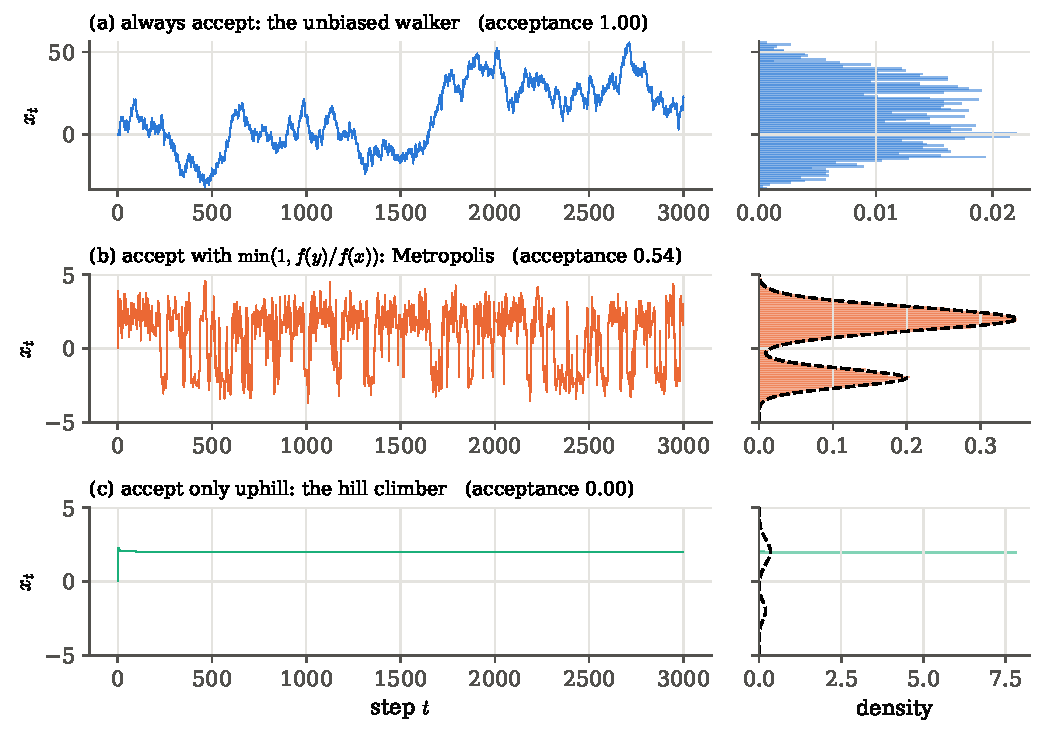
\includegraphics[width=\linewidth]{figures/ch09/biased_walker.pdf}
\caption{Three walkers with the same Gaussian proposals and three decision rules, on the
two-bump density \eqref{9b:eq:two-bumps}. Left: the first 3000 steps. Right: histograms, with the
target dashed. (a) The drunkard wanders off; its histogram is not a density of anything stable.
(b) The Metropolis walker hops between the bumps and its long-run histogram is the target.
(c) The hill climber reaches the top of the nearest bump and freezes there.}
\label{9b:fig:walkers}
\end{figure}

Why the ratio $f(y)/f(x)$, and not, say, its square? Here is the plausibility argument; the
proof comes with detailed balance (\cref{9b:sec:balance}). Suppose many walkers are already spread out as $f$, the way the crowd
of politicians was spread over the islands in proportion to the populations
(\cref{9a:sec:stationary}). Take two points $x$ and $y$ with $f(y)<f(x)$. The number of walkers
who move from $x$ to $y$ in one step is (number at $x$) $\times$ (chance of proposing $y$)
$\times$ (chance of accepting). The number moving back is (number at $y$) $\times$ (chance of
proposing $x$) $\times$ (chance of accepting). The proposal is symmetric, so the two proposal
chances are equal. The walkers at $x$ outnumber those at $y$ by $f(x)/f(y)$. For the two flows
to cancel, which is detailed balance, the acceptance from $x$ to $y$ must be smaller than the
acceptance from $y$ to $x$ by exactly the factor $f(y)/f(x)$. Accepting every uphill move and
downhill moves with probability $f(y)/f(x)$ does precisely that, and nothing else in the rule
refers to $f$.

\begin{keyidea}[The biased random walker]
A random walk alone samples nothing: it diffuses forever. What turns it into a sampler is a
bias, and the accept--reject step is that bias. Uphill proposals are always taken, a downhill
proposal is taken with probability equal to the ratio of the target densities, and a refused
proposal leaves the walker where he is for one more tick. The walker then spends more time where
the probability is higher, in exact proportion to it. Without the accept--reject step we would
simply be simulating the random walk \mainref{p.~415}.
\end{keyidea}

Written as a recipe, this is the algorithm that \textcite{Metropolis1953} published for the
statistical mechanics of interacting particles, and that \textcite{Hastings1970} generalised to
asymmetric proposals (\cref{9b:sec:hastings}).

\begin{workdef}[random-walk Metropolis]
Given a function returning $\ln f(x)$ up to a constant, a starting point $x_0$ with $f(x_0)>0$,
and a step length $s$:
\begin{enumerate}[nosep]
  \item \emph{Propose} $y=x_t+s\,z$ with $z\sim\Normal(0,1)$ \unpack{the drunkard's step, symmetric in $x$ and $y$}.
  \item \emph{Compare}: compute $R=f(y)/f(x_t)$ \unpack{the only place the target enters}.
  \item \emph{Decide}: draw $U\sim\mathrm{Uniform}(0,1)$. If $U<R$ set $x_{t+1}=y$
        \unpack{this happens with probability $\min(1,R)$}. Otherwise set $x_{t+1}=x_t$
        \unpack{the old point is recorded again, it is not skipped}.
\end{enumerate}
The list $x_0,x_1,x_2,\dots$, after the first stretch is discarded, is a correlated sample from
$f$ \mainref{pp.~411--412}, \srcref{Kruschke}{§7.3}, \srcref{Padilla}{eq.~56}.
\emph{Operational test:} the fraction of accepted proposals is between about 0.2 and 0.5, and
long runs from different starts give the same histograms (\cref{9b:sec:stepsize,9b:sec:rhat}).
\end{workdef}

\subsection{Only ratios enter: the denominator of Bayes cancels}
\label{9b:sec:ratios}

The rule needs $f(y)/f(x)$ and nothing else. To see why that is such good news, run once more
through the reasoning of \cref{ch:05} that produces a posterior, in its usual order. \emph{What
did we observe?} The whole data vector $\data$, all of it at once, is the one observed event.
\emph{What could have produced it?} Each value of the parameter vector $\params$ is a candidate
explanation, one hypothesis about how nature was set up. \emph{How readily would each have
produced it?} For every candidate the likelihood $p(\data\given\params)$ answers: had nature
been set up this way, how plausible would it have been to get exactly this $\data$?
\emph{How do we update?} Bayes' theorem multiplies that likelihood by the prior plausibility of
the candidate and divides by the evidence $Z=p(\data)$, the sum of likelihood times prior over
every candidate. That denominator is the one quantity that needs every hypothesis at once.

The walker never asks for a posterior on its own. At each tick it holds two candidate
explanations side by side, the present point and the proposal, and asks only how much more
weight one has than the other. A ratio of two weights that share the same denominator does not
contain the denominator. Write the target as the posterior of a parameter vector $\params$
given data $\data$, with likelihood $\Like(\params)=p(\data\given\params)$ and prior
$p(\params)$. For a current point $\params$ and a proposal $\params'$,
\begin{align}
  R
  &\eqby{1}\frac{p(\params'\given\data)}{p(\params\given\data)}
   \eqby{2}\frac{\Like(\params')\,p(\params')/Z}{\Like(\params)\,p(\params)/Z}
   \eqby{3}\frac{\Like(\params')\,p(\params')}{\Like(\params)\,p(\params)},
  \nonumber\\
  \ln R
  &\eqby{4}\bigl[\ln\Like(\params')+\ln p(\params')\bigr]
     -\bigl[\ln\Like(\params)+\ln p(\params)\bigr].
  \label{9b:eq:ratio}
\end{align}
\begin{explain}
  \item The target density $f$ is the posterior.
  \item Bayes' theorem (\cref{ch:05}) at each of the two points, with the same $Z=\int
        \Like(\params)\,p(\params)\,\dd\params$ in both.
  \item $Z$ does not depend on the point at which the posterior is evaluated, so it cancels.
  \item Logarithm of a ratio is a difference of logarithms; the decision $U<R$ becomes
        $\ln U<\ln R$.
\end{explain}
The walker needs ``likelihood times prior'' at two points, both of which we can always compute,
and never the integral over all points, which we usually cannot: the evidence is the same
number for both candidates, so it drops out. The same cancellation will appear in statistical mechanics,
where the target is the Boltzmann weight $e^{-E/kT}/Z$ and the normalisation $Z$ is the
partition function (\cref{9b:sec:canonical}).

\paragraph{Example: the coin.}
Kruschke's coin \srcref{Kruschke}{§7.3.1} landed heads $z=14$ times in $N=20$ flips. With a flat
prior on the bias $\theta\in(0,1)$ the posterior is
$p(\theta\given\data)=\theta^{z}(1-\theta)^{N-z}/B(z+1,N-z+1)$, where $B$ is the beta function.
From $\theta=0.6$ a proposal $\theta'=0.75$ has
\begin{align*}
  \ln R
  &\eqby{1}14\ln\frac{0.75}{0.6}+6\ln\frac{0.25}{0.4}
   \eqby{2}14\times0.2231+6\times(-0.4700)
   =3.124-2.820=0.304 ,
\end{align*}
\begin{explain}
  \item The beta function, the evidence of this problem, cancels; the flat prior is 1 at both
        points.
  \item $\ln1.25=0.2231$ and $\ln0.625=-0.4700$.
\end{explain}
so $R=e^{0.304}=1.36>1$ and the move is taken. The reverse proposal, from $0.75$ to $0.6$,
has $R=1/1.36=0.74$ and is taken 74 times in a hundred. The walker therefore sits near $0.75$ a
little more often than near $0.6$, by the factor 1.36, which is the ratio of the posterior
densities at the two points.

\paragraph{Example: why we never compute $Z$ instead.}
The evidence is a $D$-dimensional integral. A grid with $n$ points per axis costs $n^D$
evaluations, $10^{12}$ for $n=100$ and $D=6$ (\cref{ch:05}). Plain acceptance--rejection
sampling (\cref{ch:06}) does no better in many dimensions. To sample uniformly inside the unit
ball in $D$ dimensions by drawing points in the enclosing cube of side 2 and keeping those
inside, the acceptance is the volume ratio
$V_D/2^D=(\sqrt\pi/2)^D/\Gamma(1+D/2)$: $\pi/4\simeq0.79$ for $D=2$, about $0.0025$ for
$D=10$, and about $10^{-70}$ for $D=100$ \srcref{HobsonBMC}{§3.2.2, p.~61}. Most of a
high-dimensional box is corners. A walker that moves locally and only compares neighbouring
points never pays this price, because it never looks at the empty corners at all.\footnote{The
source quotes $\sim0.025$ for $n=10$; the formula it gives evaluates to
$(\sqrt\pi/2)^{10}/\Gamma(6)=0.0025$.}

\paragraph{Example: why logarithms.}
A likelihood built from many data points is a product of many factors and underflows. For a
Gaussian likelihood of $10^4$ data points with $\chi^2\simeq10^4$, $\Like\propto
e^{-\chi^2/2}=e^{-5000}$, far below the smallest positive double-precision number,
$e^{-745}\simeq5\times10^{-324}$. Every point would evaluate to zero and every ratio to $0/0$.
The difference $\ln\Like(\params')-\ln\Like(\params)=-(\chi^{\prime2}-\chi^2)/2$ is an
ordinary number of order one. Every sampler below therefore works with $\ln f$ and
accepts when $\ln U<\ln f(y)-\ln f(x)$, which is the advice of \cref{ch:05} to sum
log-likelihoods and never multiply raw ones.
\section{Why the rule is \texorpdfstring{$\min(1,R)$}{min(1,R)}: detailed balance}
\label{9b:sec:balance}

The walker of \cref{9b:sec:biased} took every uphill proposal and a downhill one with
probability $f(y)/f(x)$, and on the two-bump density \eqref{9b:eq:two-bumps} its histogram came
out right. We justified the rule with a crowd of walkers whose flows between two points cancel.
That argument used one special feature, a symmetric proposal, and it left open whether other
rules would also work. Both points matter in practice. Parameters with a boundary, such as a
rate that must be positive, need proposals that are not symmetric, and among the rules that
work we want the one that wastes the fewest proposals.

\paragraph{The question.} Fix a way of proposing moves: from $x$, a candidate $y$ is drawn from
a density $q(y\given x)$. With what probability $a(x,y)$ should we accept it so that the target
$f$ is the stationary distribution of the resulting chain?

\paragraph{The one-step law of the chain.}
Two things can happen in one step from $x$. Either a candidate $y$ is proposed \emph{and}
accepted, which has density $q(y\given x)\,a(x,y)$ in $y$; or the candidate is refused and the
chain stays at $x$. The second possibility has total probability
\begin{equation}
  r(x)=1-\int q(y\given x)\,a(x,y)\,\dd y ,
  \label{9b:eq:reject-mass}
\end{equation}
because the proposal certainly produces some $y$ and the step either accepts or refuses it.
The transition kernel of \cref{9a:sec:kernel} therefore has a smooth part and a spike at the
starting point:

\begin{workdef}[Metropolis--Hastings kernel]
The probability that one step from $x$ lands in a small set $\dd y$ is
\begin{equation}
  P(x,\dd y)=q(y\given x)\,a(x,y)\,\dd y\;+\;r(x)\,\delta_x(\dd y),
  \label{9b:eq:mh-kernel}
\end{equation}
where $\delta_x$ \unpack{the point mass at $x$, probability one on the point itself} carries the
refusals, and the acceptance probability is
\begin{equation}
  a(x,y)=\min\bigl(1,R_H(x,y)\bigr),
  \qquad
  R_H(x,y)=\frac{f(y)\,q(x\given y)}{f(x)\,q(y\given x)} .
  \label{9b:eq:hastings-ratio}
\end{equation}
$R_H$ is the \newterm{Hastings ratio} \unpack{target ratio times the ratio of the reverse to the
forward proposal density}; for a symmetric proposal, $q(x\given y)=q(y\given x)$, it
reduces to $f(y)/f(x)$ \mainref{p.~412}, \srcref{HobsonBMC}{§3.2.4, p.~63},
\srcref{Padilla}{eqs.~55--56}.
\end{workdef}

\paragraph{Deriving the acceptance from detailed balance.}
Recall from \cref{9a:sec:detailed-balance} that a chain is in \emph{detailed balance} with $f$
when the probability flow from $x$ to $y$ equals the flow from $y$ to $x$, for every pair. For
$y\ne x$ only the smooth part of \eqref{9b:eq:mh-kernel} moves probability, so we ask
\begin{align}
  f(x)\,q(y\given x)\,a(x,y)
  &\eqby{1}f(y)\,q(x\given y)\,a(y,x)
  \nonumber\\
  \iff\quad
  \frac{a(x,y)}{a(y,x)}
  &\eqby{2}\frac{f(y)\,q(x\given y)}{f(x)\,q(y\given x)}
   \eqby{3}R_H(x,y).
  \label{9b:eq:db-ratio}
\end{align}
\begin{explain}
  \item Flow from $x$ to $y$: density of being at $x$, times density of proposing $y$, times the
        chance of accepting; and the same for the reverse flow.
  \item Divide both sides by $f(x)\,q(y\given x)\,a(y,x)$, assuming these are nonzero.
  \item Definition \eqref{9b:eq:hastings-ratio}. Note that $R_H(y,x)=1/R_H(x,y)$.
\end{explain}
Detailed balance fixes only the \emph{ratio} of the two acceptances, not each one. So let the
acceptance be some function of the Hastings ratio, $a(x,y)=g\bigl(R_H(x,y)\bigr)$, with values
in $[0,1]$. Because $R_H(y,x)=1/R_H(x,y)$, condition \eqref{9b:eq:db-ratio} becomes a condition
on $g$ alone:
\begin{equation}
  g(R)=R\,g(1/R)\qquad\text{for every }R>0 .
  \label{9b:eq:g-condition}
\end{equation}
Many functions satisfy it. Two classic ones are the Metropolis choice and Barker's choice:
\begin{align*}
  g_{\rm M}(R)&=\min(1,R):
  &&\text{for }R\ge1,\;\;R\,g_{\rm M}(1/R)=R\cdot\tfrac1R=1=g_{\rm M}(R),\\
  &&&\text{for }R<1,\;\;R\,g_{\rm M}(1/R)=R\cdot1=R=g_{\rm M}(R);\\
  g_{\rm B}(R)&=\frac{R}{1+R}:
  &&R\,g_{\rm B}(1/R)=R\,\frac{1/R}{1+1/R}=\frac{R}{R+1}=g_{\rm B}(R).
\end{align*}

\paragraph{The Metropolis choice is the largest.}
Any admissible $g$ satisfies two bounds: $g(R)\le1$, because it is a probability, and
$g(R)=R\,g(1/R)\le R\cdot1=R$, by \eqref{9b:eq:g-condition} and the first bound applied to
$g(1/R)$. Hence
\begin{equation}
  g(R)\le\min(1,R)=g_{\rm M}(R)\qquad\text{for every admissible }g .
  \label{9b:eq:peskun}
\end{equation}
Metropolis accepts every proposal with the largest probability that detailed balance allows
(\cref{9b:fig:g-family}). Fewer refusals mean fewer wasted steps and less stickiness, and
\textcite{Peskun1973} showed that, for a given proposal, this choice also gives the smallest
asymptotic variance of chain averages among such rules.

\begin{figure}[htbp]
\centering
\begin{tikzpicture}
\begin{axis}[width=8.5cm,height=5.2cm,xmin=0,xmax=4,ymin=0,ymax=1.15,
  axis lines=left,xlabel={Hastings ratio $R$},ylabel={acceptance $g(R)$},
  ytick={0,0.5,1},xtick={0,1,2,3,4},legend style={draw=none,fill=none,font=\small,
  at={(0.97,0.35)},anchor=east},legend cell align=left]
  \addplot[formblue,very thick,domain=0:4,samples=200] {min(1,x)};
  \addlegendentry{Metropolis, $\min(1,R)$}
  \addplot[fibreorange,thick,domain=0:4,samples=200] {x/(1+x)};
  \addlegendentry{Barker, $R/(1+R)$}
  \addplot[faint,dashed,domain=0:1.15] {x};
  \addplot[faint,dashed,domain=0:4] {1};
\end{axis}
\end{tikzpicture}
\caption{Two acceptance rules that both satisfy detailed balance. Every admissible rule lies
below the line $g=R$ and below $g=1$ (both dashed); the Metropolis rule runs along these two
bounds, so it refuses as few proposals as possible.}
\label{9b:fig:g-family}
\end{figure}

\paragraph{From detailed balance to stationarity, with the refusals included.}
Detailed balance \eqref{9b:eq:db-ratio} concerns $y\ne x$. The refusals in
\eqref{9b:eq:mh-kernel} keep probability at $x$, and they must be counted when we check that $f$
is stationary, that is, that a crowd of walkers spread as $f$ is still spread as $f$ after one
step. The density of walkers at $y$ after the step is the flow into $y$ from everywhere else plus
the walkers already at $y$ who stayed:
\begin{align}
  \int f(x)\,q(y\given x)\,a(x,y)\,\dd x+f(y)\,r(y)
  &\eqby{1}\int f(y)\,q(x\given y)\,a(y,x)\,\dd x+f(y)\,r(y)
  \nonumber\\
  &\eqby{2}f(y)\Bigl[\int q(x\given y)\,a(y,x)\,\dd x+r(y)\Bigr]
   \eqby{3}f(y).
  \label{9b:eq:mh-stationary}
\end{align}
\begin{explain}
  \item Detailed balance \eqref{9b:eq:db-ratio} for each pair $(x,y)$ inside the integral.
  \item $f(y)$ does not depend on the integration variable $x$.
  \item By \eqref{9b:eq:reject-mass} at the point $y$, the probability of leaving $y$ plus the
        probability of staying is one.
\end{explain}
Wasserman checks \eqref{9b:eq:db-ratio} case by case \mainref{pp.~413--414, (24.7)--(24.9)}: if
$f(x)q(y\given x)>f(y)q(x\given y)$, then $a(x,y)=R_H<1$ and $a(y,x)=1$, so
$f(x)\,q(y\given x)\,a(x,y)=f(y)\,q(x\given y)=f(y)\,q(x\given y)\,a(y,x)$; the other case is the
same with $x$ and $y$ exchanged.

Stationarity is half of what a sampler needs; the other half is that the chain actually gets
there from any start. The results of \cref{9a:sec:convergence,9a:sec:ergodic} supply it once the
chain is irreducible and aperiodic. A Gaussian proposal has $q(y\given x)>0$ for every $y$, so
any region where $f>0$ can be reached in a single step: the chain is irreducible. And whenever
some proposals are refused, the chain can stay put, which removes any cycle: it is aperiodic.
Then the distribution of $X_t$ converges to $f$ from any starting point, and chain averages
converge to averages over $f$ (the ergodic theorem, \cref{9a:sec:ergodic}).\footnote{For a
continuous state space the full statement needs a little more measure theory (Harris
recurrence); for the targets of this book, with $f$ continuous and positive on a connected
region and Gaussian proposals, it holds.}

\paragraph{Example: two states, Metropolis against Barker.}
Take two states with target $f=(\tfrac13,\tfrac23)$ and a proposal that always suggests the
other state, so $q$ is symmetric and the Hastings ratio is just the target ratio. A walker in
state 1 is offered state 2, with $R=f_2/f_1=2$; a walker in state 2 is offered state 1, with
$R=f_1/f_2=\tfrac12$. Each rule turns these two ratios into acceptance probabilities:
\begin{align*}
  \text{from state 1 }(R=2):&\quad a_{\rm M}\eqby{1}\min(1,2)=1,
  &a_{\rm B}&\eqby{2}\frac{2}{1+2}=\frac23,\\
  \text{from state 2 }(R=\tfrac12):&\quad a_{\rm M}\eqby{1}\min\bigl(1,\tfrac12\bigr)=\tfrac12,
  &a_{\rm B}&\eqby{2}\frac{1/2}{1+1/2}=\frac13 .
\end{align*}
\begin{explain}
  \item The Metropolis rule $g_{\rm M}(R)=\min(1,R)$.
  \item Barker's rule $g_{\rm B}(R)=R/(1+R)$.
\end{explain}
An accepted proposal switches state; a refused one keeps it, so each row of the transition
matrix is (refuse, accept) or (accept, refuse). With rows labelled by where the walker is and
columns by where it goes,
\begin{equation*}
  P_{\rm M}=\begin{pmatrix}0&1\\ \tfrac12&\tfrac12\end{pmatrix},
  \qquad
  P_{\rm B}=\begin{pmatrix}\tfrac13&\tfrac23\\ \tfrac13&\tfrac23\end{pmatrix}.
\end{equation*}
Both leave $f$ unchanged: $(\tfrac13,\tfrac23)P_{\rm M}=(\tfrac13,\tfrac23)$, and every row of
$P_{\rm B}$ is already $f$.

\emph{Which is the better sampler?} Both are correct, so the question is how many steps each
needs for a given precision. The two-state chain with $p_{12}=a$ and $p_{21}=b$ has
autocorrelation $\lambda^k$ with $\lambda=1-a-b$ and integrated autocorrelation time
$\tau=(1+\lambda)/(1-\lambda)$, from \eqref{9a:eq:tau-two}. Barker has $a=\tfrac23$,
$b=\tfrac13$, $\lambda=0$ and $\tau=1$: its draws are independent. Metropolis has $a=1$,
$b=\tfrac12$, $\lambda=-\tfrac12$ and
\begin{equation*}
  \tau_{\rm M}=\frac{1-\tfrac12}{1+\tfrac12}=\frac13 .
\end{equation*}
\emph{What $\tau$ buys.} The variance of a chain average is $\sigma^2\tau/N$ by
\eqref{9a:eq:var-time-average}, where $\sigma^2$ is the variance of one value. Independent draws
have $\tau=1$, so $N_{\rm ind}$ of them give $\sigma^2/N_{\rm ind}$. The two variances are equal
when $N_{\rm ind}=N/\tau$, which for $\tau_{\rm M}=\tfrac13$ is $3N$: $N$ Metropolis steps
estimate the fraction of time in state 1 as well as $3N$ independent draws would.

\emph{Why the chain beats independence.} From state 1 the move to state 2 is uphill, and
Metropolis never refuses an uphill move, so the walker leaves state 1 at every visit. The chain
switches state as often as detailed balance allows, and a value in state 1 is followed by a
value in state 2 more often than chance would have it. Successive values are anticorrelated
($\lambda<0$), and their errors in the running average partly cancel instead of adding up.
Barker refuses the uphill move one time in three and loses this. The general statement, proved
by \textcite{Peskun1973} for any target and any fixed proposal, is that a rule which refuses
less never gives a larger asymptotic variance; the two-state matrices above are that theorem
in its smallest case.

\paragraph{Example: the tempered family.}
What if the walker accepts with probability $\min\bigl(1,R^\beta\bigr)$ for some exponent
$\beta\ge0$? Since
\begin{equation*}
  R^\beta=\Bigl(\frac{f(y)}{f(x)}\Bigr)^\beta=\frac{f(y)^\beta}{f(x)^\beta},
\end{equation*}
this is exactly the Metropolis rule for the target $f^\beta$, so by \eqref{9b:eq:mh-stationary}
the walker samples $f^\beta/\!\int f^\beta$. The family interpolates between the two failures of
\cref{9b:sec:biased}: $\beta=0$ is the drunkard ($f^0=1$ is flat and not normalisable on the
line) and $\beta\to\infty$ is the hill climber ($f^\beta$ piles up at the highest point).
\Cref{9b:fig:tempered} checks the claim on the two-bump density with $2\times10^5$ steps: the
fraction of time at $x>0$ is $\NineBBwRightLow$ for $\beta=0.3$ (exact, from $f^{0.3}$ normalised
on a grid: $\NineBBwRightExactLow$), $\NineBBwRightOne$ for $\beta=1$ ($\NineBBwRightExactOne$) and
$\NineBBwRightThree$ for $\beta=3$ ($\NineBBwRightExactThree$). If $f=e^{-E}$ then
$f^\beta=e^{-\beta E}$, a Boltzmann weight at temperature $1/\beta$: lowering $\beta$ heats the
target and flattens its barriers. Simulated annealing (raising $\beta$ slowly to find a global
maximum) and parallel tempering (running several $\beta$ at once and swapping) are built on this
observation; the temperature returns as a physical temperature in \cref{9b:sec:canonical}.

\begin{figure}[htbp]
\centering
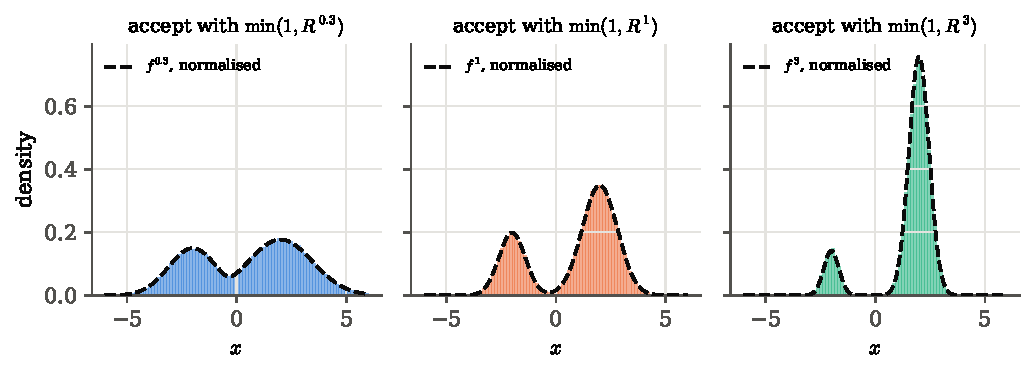
\includegraphics[width=\linewidth]{figures/ch09/tempered_family.pdf}
\caption{A walker that accepts with $\min(1,R^\beta)$ samples $f^\beta$, not $f$. Histograms of
three such walkers on the two-bump density, with $f^\beta$ normalised on a grid (dashed). Small
$\beta$ flattens the target towards the drunkard's flat line; large $\beta$ sharpens it towards
the hill climber's spike.}
\label{9b:fig:tempered}
\end{figure}

\subsection{Asymmetric proposals: the Hastings factor}
\label{9b:sec:hastings}

A Poisson process gave $n=2$ events in unit exposure. With a flat prior on the rate $\lambda>0$,
the posterior is $f(\lambda)\propto\lambda^2e^{-\lambda}$, a Gamma density with shape 3, mean 3,
and probability $\NineBHbLowExact$ below $\lambda=0.5$. Rates, variances, masses and amplitudes
all live on a half-line, and near the wall at $\lambda=0$ a Gaussian proposal of width $s=2$
often suggests a negative rate.

\paragraph{The question.} What should the walker do with a proposal on the wrong side of the
wall, and what changes if we choose proposals that never cross it?

We try five samplers, each run for $\NineBHbN$ steps (\cref{9b:fig:hastings}), and ask of each
whether it satisfies \eqref{9b:eq:db-ratio}.

\emph{A: Gaussian step, stay put if $y<0$.} The target is $f(y)=0$ there, so $R=0$ and the
proposal is refused like any other bad proposal. Nothing about the rule has changed, so it is
exact: mean $\NineBHbMeanA$, and a fraction $\NineBHbLowA$ of the time below 0.5.

\emph{B: Gaussian step, redraw until $y>0$, no correction.} This feels harmless but changes the
proposal. \emph{The redrawn proposal density.} An untruncated step $y=x+sZ$ has density
$\phi\bigl((y-x)/s\bigr)/s$, where $\phi$ and $\Phi$ are the standard Gaussian density and
cumulative distribution. The step lands on the allowed side with probability
$\Prob(x+sZ>0)=\Prob(Z>-x/s)=\Phi(x/s)$, the last step because $Z$ is symmetric about zero.
Redrawing until $y>0$ keeps only those draws, so it renormalises the Gaussian over $y>0$ by
dividing by that probability:
\begin{equation}
  q(y\given x)=\frac{\phi\bigl((y-x)/s\bigr)}{s\,\Phi(x/s)},\qquad y>0.
  \label{9b:eq:trunc-q}
\end{equation}
Close to the wall, $\Phi(x/s)$ is near $\tfrac12$ (half of all steps are thrown back); far from
it, $\Phi(x/s)$ is near 1. So the denominator differs between the two directions of a move.

\emph{Which flow is unbalanced?} Take a point $x$ near the wall and a point $y$ farther out.
Sampler B accepts with $\min\bigl(1,f(y)/f(x)\bigr)$, as if the proposal were symmetric. The
two flows of \eqref{9b:eq:db-ratio} are then
\begin{align*}
  \frac{\text{flow }x\to y}{\text{flow }y\to x}
  &\eqby{1}\frac{f(x)\,q(y\given x)\min\bigl(1,f(y)/f(x)\bigr)}
               {f(y)\,q(x\given y)\min\bigl(1,f(x)/f(y)\bigr)}
   \eqby{2}\frac{q(y\given x)\,\min\bigl(f(x),f(y)\bigr)}{q(x\given y)\,\min\bigl(f(y),f(x)\bigr)}
   \eqby{3}\frac{\Phi(y/s)}{\Phi(x/s)} .
\end{align*}
\begin{explain}
  \item Density at the start, times the proposal density, times the acceptance, for each
        direction.
  \item Take $f(x)$ and $f(y)$ inside the minimum: $f(x)\min(1,f(y)/f(x))=\min(f(x),f(y))$.
  \item The two minima are the same number. In the ratio of the two densities
        \eqref{9b:eq:trunc-q} the $\phi$ factors are equal, because $\phi$ is even, and only the
        denominators are left.
\end{explain}
For $x$ nearer the wall than $y$, $\Phi(y/s)>\Phi(x/s)$ and the ratio exceeds one. With $s=2$,
$x=0.2$ and $y=2$ it is $\Phi(1)/\Phi(0.1)=0.841/0.540\simeq1.56$: probability leaves the
neighbourhood of the wall about one and a half times as fast as it comes back. Detailed balance
fails in one direction for every such pair, so the walker settles into a stationary law that is
depleted near zero. That is what the run measures: it spent only $\NineBHbLowB$ of its time below
0.5, and its mean came out at $\NineBHbMeanB$.

\emph{C: as B, with the Hastings factor.} From \eqref{9b:eq:trunc-q}, the $\phi$ factors are
equal because $\phi$ is even, and
\begin{equation*}
  \frac{q(x\given y)}{q(y\given x)}
  =\frac{\phi\bigl((x-y)/s\bigr)/[s\,\Phi(y/s)]}{\phi\bigl((y-x)/s\bigr)/[s\,\Phi(x/s)]}
  =\frac{\Phi(x/s)}{\Phi(y/s)} .
\end{equation*}
Multiplying the target ratio by this factor, as \eqref{9b:eq:hastings-ratio} instructs, restores
balance: mean $\NineBHbMeanC$, fraction below 0.5 $\NineBHbLowC$.

\emph{D: multiplicative steps with the Hastings factor.} Propose $y=x\,e^{\sigma Z}$ with
$\sigma=1$ and $Z\sim\Normal(0,1)$: a Gaussian step in $\ln\lambda$, which can never cross zero.
This is Lambert's log-normal proposal \srcref{Lambert}{§13.8}. Its density is
\begin{align}
  q(y\given x)
  &\eqby{1}\frac{1}{y\,\sigma\sqrt{2\pi}}\exp\Bigl[-\frac{(\ln y-\ln x)^2}{2\sigma^2}\Bigr],
  \nonumber\\
  \frac{q(x\given y)}{q(y\given x)}
  &\eqby{2}\frac{1/x}{1/y}
   =\frac{y}{x}.
  \label{9b:eq:lognormal-factor}
\end{align}
\begin{explain}
  \item $\ln y=\ln x+\sigma Z$ is Gaussian; the density of $y$ picks up the Jacobian
        $\abs{\dd\ln y/\dd y}=1/y$ (change of variables, \cref{ch:02}).
  \item The exponential is symmetric in $x$ and $y$ and cancels; only the Jacobian factors
        remain.
\end{explain}
With the factor $y/x$ the sampler is exact: mean $\NineBHbMeanD$, fraction below 0.5
$\NineBHbLowD$.

\emph{E: as D, without the factor.} Here the walker uses $\min\bigl(1,f(y)/f(x)\bigr)$ although
the proposal is not symmetric in $\lambda$. What does it sample? In the variable $u=\ln\lambda$
the proposal $u\to u+\sigma Z$ \emph{is} symmetric, and the decision uses $f(e^{u'})/f(e^u)$. So,
as a chain in $u$, it is an honest Metropolis sampler of the density $h(u)\propto f(e^u)$. Back
in $\lambda$,
\begin{align}
  p_E(\lambda)
  &\eqby{1}h(\ln\lambda)\,\Bigl\lvert\frac{\dd u}{\dd\lambda}\Bigr\rvert
   \eqby{2}\frac{f(\lambda)}{\lambda}
   \eqby{3}\lambda\,e^{-\lambda} .
  \label{9b:eq:no-hastings}
\end{align}
\begin{explain}
  \item Change of variables from $u$ to $\lambda=e^u$.
  \item $h(\ln\lambda)\propto f(\lambda)$ and $\dd u/\dd\lambda=1/\lambda$.
  \item $f(\lambda)\propto\lambda^2e^{-\lambda}$.
\end{explain}
The forgotten factor costs one power of $\lambda$: the walker samples a Gamma density with shape 2
and mean 2. It returned mean $\NineBHbMeanE$ and fraction $\NineBHbLowE$ below 0.5, against
$1-1.5\,e^{-0.5}=0.090$ for that wrong target. The Hastings factor is the Jacobian of the
proposal's own geometry; leaving it out is the same mistake as forgetting a Jacobian when
changing variables. This is also Wasserman's advice for bounded parameters, ``transform to
$\ln X$'' \mainref{p.~415}: sampling $u=\ln\lambda$ with symmetric steps is fine provided the
target in $u$ includes the Jacobian, $h(u)=f(e^u)\,e^u$, which is exactly the factor $y/x$ of D.

\begin{figure}[htbp]
\centering
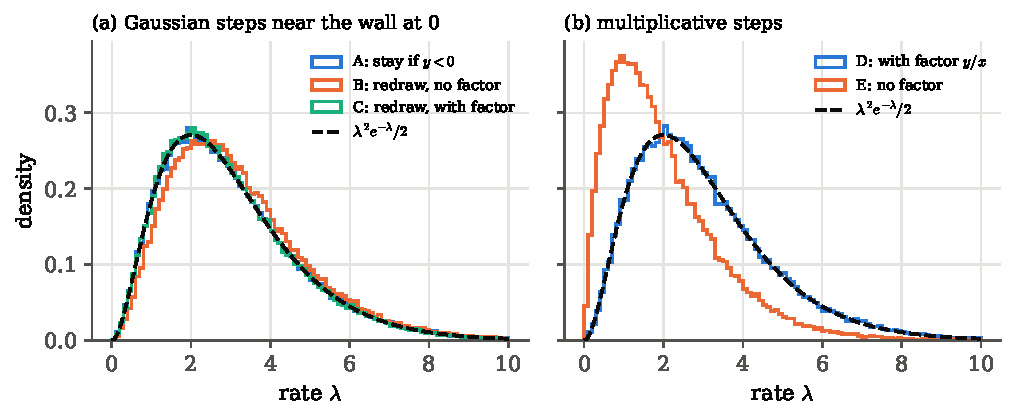
\includegraphics[width=\linewidth]{figures/ch09/hastings_boundary.pdf}
\caption{Five ways to sample a positive rate with posterior $\lambda^2e^{-\lambda}/2$ (dashed).
(a) Gaussian steps: staying put when the step crosses zero (A) and redrawing with the Hastings
factor (C) are exact; redrawing without it (B) pushes the walker away from the wall. (b)
Multiplicative steps: with the factor $y/x$ (D) exact; without it (E) the walker samples
$\lambda e^{-\lambda}$, with one power of $\lambda$ missing.}
\label{9b:fig:hastings}
\end{figure}

Sampler A deserves a remark because one textbook warns against it. Lambert writes that if all
steps proposing a negative value are rejected, too few samples are generated near zero
\srcref{Lambert}{§13.8}.\footnote{Lambert's statement and Fig.~13.15 describe what happens when the
negative proposals are \emph{discarded and redrawn}, which is our sampler B. If the walker stays
where it is and records the current point again, which is how every Metropolis step treats a
refusal, the region near zero is sampled correctly; sampler A agrees with the exact answer.}
What goes wrong is redrawing, not refusing.

\begin{pitfall}[A refusal repeats the current point]
In acceptance--rejection sampling (\cref{ch:06}, \srcref{Cowan}{§3.3}) a rejected candidate is
thrown away and a fresh independent one is drawn. In Metropolis--Hastings a refused proposal
means the walker stays, and the current point is written into the chain \emph{again}. The repeats
are not a nuisance: they are how a high-density point earns its extra weight, by being hard to
leave. Recording only the accepted moves, or redrawing until something is accepted, removes
that weight and biases every average towards low-density regions
\srcref{Padilla}{§4.1.1, step 4}.
\end{pitfall}

\paragraph{Example: the independence sampler.}
The proposal need not depend on $x$ at all. Draw every candidate from a fixed density $g$, so
$q(y\given x)=g(y)$. Then \eqref{9b:eq:hastings-ratio} gives
\begin{equation}
  R_H(x,y)=\frac{f(y)\,g(x)}{f(x)\,g(y)}=\frac{w(y)}{w(x)},\qquad w\equiv\frac fg ,
  \label{9b:eq:independence}
\end{equation}
the ratio of the importance weights of \cref{ch:06} at the candidate and at the current point
\mainref{p.~415}. A candidate with a larger weight than the current point is always accepted;
one with a smaller weight sometimes. When $g=f$ every weight is equal and every proposal is
accepted: the chain becomes independent sampling. When $g$ has thinner tails than $f$, a walker
that reaches the tail finds $w(x)$ huge and refuses almost everything for a very long time;
for exactly the reason given in \cref{ch:06} for importance sampling, $g$ must have heavier tails
than $f$.
\section{The sampler in a dozen lines, and two textbook runs}
\label{9b:sec:code}

The biased walker of \cref{9b:sec:biased} needs three operations per step: a Gaussian kick, one
evaluation of $\ln f$, and one uniform number. That fits in a short function, and the same
function will drive every chain in the rest of the book: the straight-line fit and the CMB
likelihood that follow, the comparison with the Fisher matrix in \cref{ch:10}, and the
topological summaries of \cref{ch:12}. Before trusting it with any of those, we run it on two
published examples whose numbers we did not choose, Wasserman's Cauchy chains and Kruschke's
coin.

\pyfile[firstline=25,lastline=49]{code/ch09/lib_mcmc.py}{Random-walk Metropolis, the core of
\pyname{lib_mcmc.py}}

The function follows the working definition of \cref{9b:sec:biased} line by line, with four
practical choices.
\begin{itemize}[itemsep=1pt]
  \item The target enters only through \pyname{logp}, the log density up to a constant. A point
        outside the support returns $-\infty$; then $\ln U<-\infty$ is false and the proposal
        is refused, which is sampler A of \cref{9b:sec:hastings}.
  \item The proposal is $y=x+s\,L z$ with $z$ a vector of independent standard Gaussians and
        $L$ the Cholesky factor of a matrix $\Cmat$, so $LL\T=\Cmat$. Its covariance is
        $\Cov(sLz)=s^2L\,\Cov(z)\,L\T=s^2LL\T=s^2\Cmat$. With no $\Cmat$ given, the steps are
        round; shaping them like the target is the subject of \cref{9b:sec:stepsize}.
  \item All Gaussian kicks and all uniform numbers are drawn at once before the loop. Only the
        decision, which depends on where the walker is, has to be sequential.
  \item The value of $\ln f$ at the current point is stored, so each step costs exactly one
        evaluation of the target, at the proposal. In a cosmological analysis that evaluation
        is a full likelihood call, and the number of steps is the cost of the analysis.
\end{itemize}
A refused step writes the current point again (the last line of the loop). The companion function \pyname{mh} in the
same file takes any proposal together with its log density \pyname{log_q} and adds
$\ln q(x\given y)-\ln q(y\given x)$ to the log ratio, which is the Hastings factor of
\eqref{9b:eq:hastings-ratio}; samplers C, D and E of \cref{9b:sec:hastings} used it.

\begin{pitfall}[Start where the target is positive]
Follow what the function does if the starting point has $f(x_0)=0$. Its stored log density is
then $\ln f(x_0)=-\infty$. If a proposal $y$ lands where $f(y)>0$, the log ratio is the finite
number $\ln f(y)$ minus $-\infty$, which is $+\infty$; the test $\ln U<+\infty$ is true, the move is
taken, and from then on the walker is inside the support and everything is normal. But if the
proposal also lands where $f=0$, the log ratio is $(-\infty)-(-\infty)$, which floating-point
arithmetic returns as \texttt{NaN} (``not a number''). Every comparison with \texttt{NaN} is
false, so $\ln U<\texttt{NaN}$ is false and the proposal is refused, without any warning. A start
outside the support with steps too short to reach it, say $\theta_0=-1$ for a coin bias with
steps of 0.02, therefore refuses every proposal: the trace is a flat line and the acceptance is
exactly zero. The same happens inside the support if $\ln f$ underflows to $-\infty$ at the start
and at all its neighbours. Always start where the posterior is positive
\srcref{Kruschke}{§7.3}: inside the prior range, with a finite likelihood.
\end{pitfall}

\subsection{Wasserman's Cauchy chains}
\label{9b:sec:wasserman-cauchy}

Wasserman's first MCMC example \mainref{pp.~412--413, Ex.~24.10} makes one point. A
Metropolis chain samples a density we cannot draw from directly, and it is correct for every
proposal width; but how quickly its histogram comes to resemble the target depends on that width,
and a badly chosen width wastes most of the run. He judges this by eye: a chain \emph{mixes well}
when its trace wanders over the whole range of the target without creeping or sticking. As target
he takes the Cauchy density of \cref{ch:02},
\begin{equation*}
  f(x)=\frac{1}{\pi(1+x^2)},
\end{equation*}
which is a good test for two reasons: every property of it is known exactly, so any run can be
checked, and its tails are heavy, so a sampler has to reach far from the centre to get it right.

\emph{The ratio the walker uses.} His proposal is a Gaussian step, $y\sim\Normal(x,b^2)$, with $b$
the step width. It is symmetric, so the acceptance needs only the target ratio:
\begin{align*}
  R=\frac{f(y)}{f(x)}
  &\eqby{1}\frac{1/[\pi(1+y^2)]}{1/[\pi(1+x^2)]}
   \eqby{2}\frac{1+x^2}{1+y^2}.
\end{align*}
\begin{explain}
  \item The Cauchy density at the proposal and at the present point.
  \item The $\pi$ cancels, like every normalisation (\cref{9b:sec:ratios}); dividing by a fraction
        is multiplying by its inverse.
\end{explain}
A proposal nearer the centre than $x$ has $R>1$ and is always taken; one farther out is taken
with probability $(1+x^2)/(1+y^2)$, which falls like $1/y^2$ for a long jump.

\emph{The setup.} Wasserman runs three chains that differ only in the width:
\begin{center}
\begin{tabular}{lccc}
\toprule
 & small width & middle width & large width\\
\midrule
proposal width $b$ & 0.1 & 1 & 10 \\
steps $N$ & 1000 & 1000 & 1000 \\
start & $x_0=0$ & $x_0=0$ & $x_0=0$ \\
\bottomrule
\end{tabular}
\end{center}
The start is at the centre of the target, so there is no burn-in to discard: everything that goes
wrong is caused by the width. The width $0.1$ is a tenth of the half-width of the Cauchy peak, and
$10$ is ten times it.

\emph{A number to check against.} The trace plots of his Fig.~24.2 carry no numbers, so we need
one that a run can be checked with. A convenient one is the fraction of time spent at
$\abs x<1$, whose exact value is
\begin{align*}
  \Prob(\abs X<1)
  &\eqby{1}\int_{-1}^{1}\frac{\dd x}{\pi(1+x^2)}
   \eqby{2}\frac{1}{\pi}\bigl[\arctan x\bigr]_{-1}^{1}
   =\frac1\pi\Bigl(\frac\pi4+\frac\pi4\Bigr)=\frac12 .
\end{align*}
\begin{explain}
  \item Probability of an interval is the integral of the density over it.
  \item $\dd(\arctan x)/\dd x=1/(1+x^2)$.
\end{explain}

\emph{What we compute.} The script \pyname{13_textbook_chains.py} calls the function
\pyname{metropolis} listed above with the log target $-\ln(1+x^2)$ (the constant $-\ln\pi$ is
dropped), the start $[0]$, and each width in turn. For each width it makes two runs: one of 1000
steps, as Wasserman did, and one of $2\times10^5$ steps. From each it records the fraction of
steps with $\abs x<1$, and from the long run also the acceptance rate and the integrated
autocorrelation time $\tau$ of the indicator of $\abs x<1$ (\cref{9a:sec:time-average-variance},
estimated as in \cref{9b:sec:tau}). A chain of $N$ steps with correlation time $\tau$ is worth
$N/\tau$ independent draws.

\emph{Side by side.} \Cref{9b:fig:cauchy} shows our three 1000-step chains, laid out as in his
Fig.~24.2, and the table puts his verdicts next to our numbers.
\begin{center}
\begin{tabular}{lccc}
\toprule
proposal width $b$ & 0.1 & 1 & 10 \\
\midrule
Wasserman, Fig.~24.2 (by eye) & explores little & mixes well & often stuck \\
ours, 1000 steps: time at $\abs x<1$ & $\NineBCauHalfSmall$ & $\NineBCauHalfOne$ & $\NineBCauHalfBig$ \\
ours, $2\times10^5$ steps: time at $\abs x<1$ & $\NineBCauHalfLongSmall$ & $\NineBCauHalfLongOne$ & $\NineBCauHalfLongBig$ \\
ours, $2\times10^5$ steps: acceptance & $\NineBCauAccSmall$ & $\NineBCauAccOne$ & $\NineBCauAccBig$ \\
ours, $2\times10^5$ steps: $\tau$ (steps) & $\NineBCauTauSmall$ & $\NineBCauTauOne$ & $\NineBCauTauBig$ \\
\bottomrule
\end{tabular}
\end{center}
The traces have the features he describes. With $b=0.1$ the walker takes tiny steps and is still
exploring the centre after 1000 of them, so it spends far too much time at $\abs x<1$. With
$b=10$ most proposals land far out in the tail and are refused, and the trace is a staircase of
long flat stretches. The $b=1$ chain looks the liveliest. But in our run it happened to make a
long excursion into a tail and spent only $\NineBCauHalfOne$ of its time at $\abs x<1$, further
from the exact $\tfrac12$ than the ``stuck'' $b=10$ chain.

\begin{figure}[htbp]
\centering
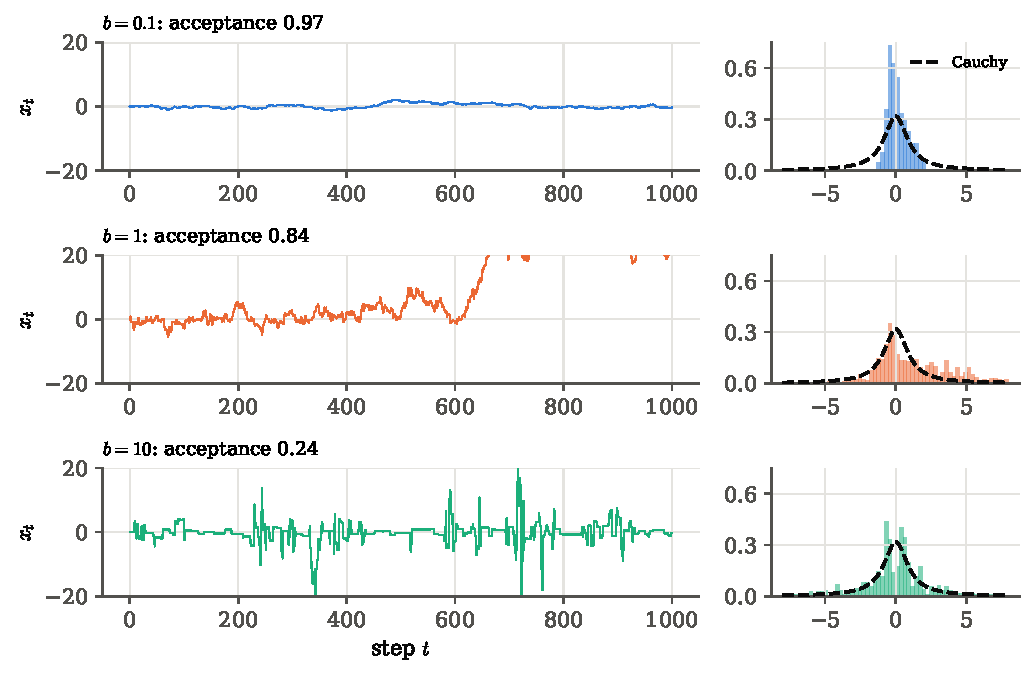
\includegraphics[width=\linewidth]{figures/ch09/cauchy_chains.pdf}
\caption{Wasserman's Cauchy example: three Metropolis chains of 1000 steps with proposal widths
$b=0.1$, $1$ and $10$ (left), and their histograms with the Cauchy density (right). Small steps
creep; large steps are mostly refused and the trace has flat stretches; in 1000 steps no
histogram is yet a good copy of the target.}
\label{9b:fig:cauchy}
\end{figure}

\emph{Why the verdicts differ.} A 1000-step run cannot carry the weight of a ranking. The
statistical error of a chain average is $\sigma\sqrt{\tau/N}$ (\cref{9b:sec:tau}). For the
fraction of time at $\abs x<1$, an average of an indicator that is 1 half the time, $\sigma=\tfrac12$.
With $N=1000$ and the long-run $\tau$ values of the table, the error is
$\tfrac12\sqrt{\NineBCauTauOne/1000}\simeq0.08$ for $b=1$ and
$\tfrac12\sqrt{\NineBCauTauBig/1000}\simeq0.06$ for $b=10$: two widths whose $\tau$ differ by
less than a factor of two cannot be told apart by one short run, and any single 1000-step
histogram, his or ours, is a noisy copy of the target. Only $b=0.1$, whose $\tau$ is some thirty
times larger, is clearly worse in 1000 steps, and that part of his verdict stands.

The long runs are close to converged (each fraction is within two of its errors of $\tfrac12$), and they rank the
other two the other way round: $b=10$ has the shorter $\tau$, so it is at least as good as $b=1$
although it refuses three proposals in four. The reason is the Cauchy tail:
$\Prob(\abs X>10)=1-\tfrac2\pi\arctan10=0.063$, so six per cent of the probability sits beyond
$\abs x=10$, and only long jumps reach it in reasonable time. A walker with $b=1$ has to diffuse
out there one unit at a time and back again, which is the long excursion its short trace shows.
A good step length depends on the shape of the target, not only on the width of its peak.

Note also what we did \emph{not} estimate: the mean of a Cauchy variable does not exist
(\cref{ch:02}), and a chain average of $x$ would wander forever however well the chain mixes. A
sampler cannot create a moment the distribution does not have.

\emph{The lesson.} A thousand steps judged by eye can tell a creeping chain from a working one,
but they cannot rank two working samplers; that takes $\tau$ from a long run.

\subsection{Kruschke's coin}
\label{9b:sec:kruschke-coin}

Kruschke's first Metropolis run \srcref{Kruschke}{§7.3.1, Fig.~7.4} answers a question every
user of the method has at the start. A coin was flipped $N=20$ times and landed heads $z=14$
times. We want the posterior for its bias $\theta$, the probability of heads, and we do not want
to integrate anything: can a walker that only ever compares two values of $\theta$ produce that
posterior, and what does the choice of proposal width do to the result?

\emph{The exact answer, for checking.} With the flat prior $\mathrm{Beta}(\theta;1,1)$ the
posterior can be written down, which is why the problem makes a good test:
\begin{align*}
  p(\theta\given\data)
  &\eqby{1}\frac{\theta^{14}(1-\theta)^{6}\cdot1}{\int_0^1t^{14}(1-t)^6\,\dd t}
   \eqby{2}\mathrm{Beta}(\theta;15,7),
\end{align*}
\begin{explain}
  \item Bernoulli likelihood $\theta^z(1-\theta)^{N-z}$ times a flat prior, normalised.
  \item The normalised density $\propto\theta^{a-1}(1-\theta)^{b-1}$ is the beta density with
        $a=15$, $b=7$ (\cref{ch:05}); its mean is $a/(a+b)=15/22=0.6818$ and its standard
        deviation is $0.097$.
\end{explain}
The walker does not use this formula. It receives only the log target $14\ln\theta+6\ln(1-\theta)$
inside $(0,1)$ and $-\infty$ outside, and the integral in the denominator never appears
(\cref{9b:sec:ratios}).

\emph{A deliberately bad start.} Kruschke starts every chain at $\theta=0.01$, far in the left
tail: the posterior density there is smaller than at the mean by a factor
\begin{equation*}
  \frac{f(0.01)}{f(0.68)}=\exp\Bigl[14\ln\frac{0.01}{0.68}+6\ln\frac{0.99}{0.32}\Bigr]\simeq e^{-52}.
\end{equation*}
A start there shows the walker finding the posterior before it explores it, the burn-in of
\cref{9b:sec:burnin}, and how long that takes for each width.

\emph{Three widths.} Each chain runs $50\,000$ steps, and only the width $s$ of the Gaussian
proposal changes. Compared with the posterior width of about $0.1$:
\begin{itemize}[itemsep=1pt]
  \item $s=0.02$ is a fifth of the posterior width. Almost every step is a small move to a point of
        nearly the same density, so almost every step is accepted, but the walker covers ground
        only by diffusion and creeps.
  \item $s=0.2$ is about twice the posterior width. A proposal lands in a region of quite
        different density about as often as not, so roughly half are taken, and each accepted move
        is a real jump across the posterior.
  \item $s=2$ is twenty times the posterior width, and twice the whole allowed interval. Most
        proposals land outside $(0,1)$, where the target is zero, or far down a tail, and are
        refused; the walker sits still for long stretches.
\end{itemize}
For each chain Kruschke reports two numbers: the acceptance rate, and the \newterm{effective
sample size} $\mathrm{ESS}=N/\tau$, the number of independent draws that would give the posterior
mean as accurately as the $N$ correlated steps do, with $\tau$ the integrated autocorrelation
time (defined in full, with its estimator, in \cref{9b:sec:tau}).

\emph{Side by side.} Our runs use the same start, widths and length, with our own random numbers:
\begin{center}
\begin{tabular}{lccc}
\toprule
proposal width & 0.02 & 0.2 & 2 \\
\midrule
acceptance, ours & $\NineBCoinAccSmall$ & $\NineBCoinAccMid$ & $\NineBCoinAccBig$ \\
acceptance, Kruschke & $\NineBCoinKrAccSmall$ & $\NineBCoinKrAccMid$ & $\NineBCoinKrAccBig$ \\
effective size, ours & $\NineBCoinEssSmall$ & $\NineBCoinEssMid$ & $\NineBCoinEssBig$ \\
effective size, Kruschke & $\NineBCoinKrEssSmall$ & $\NineBCoinKrEssMid$ & $\NineBCoinKrEssBig$ \\
\bottomrule
\end{tabular}
\end{center}

\emph{How close should they be?} Two runs with different random numbers cannot agree exactly; the
question is how far apart chance alone puts them. The acceptance rate is an average of $N$
accept-or-refuse indicators, with a spread of order $\sqrt{a(1-a)/N}\simeq0.002$ for $a=0.5$ and
$N=50\,000$, a little more because successive decisions are correlated; the three pairs differ by
a few thousandths. The estimated $\tau$, and hence the ESS, has a relative spread of about
$\sqrt{2(2M+1)/N}$ from one random-number stream to another, with $M\simeq5\tau$ the window of
the estimate \eqref{9b:eq:tau-noise}. With $\tau=N/\mathrm{ESS}$ from the table, that is about
$4\%$ for width 0.2 (an ESS spread of $\pm500$), $10\%$ for width 2 ($\pm200$) and $20\%$ for width
0.02 ($\pm100$). The three ESS pairs differ by about $540$, $50$ and $6$: all within what a second
stream would give. Kruschke's ESS also comes from a different
estimator (the \pyname{coda} package of R), which adds a few per cent of its own.

\emph{What each walker did.} The 0.02 walker needs hundreds of steps to crawl from $0.01$ to the
bulk of the posterior (\cref{9b:fig:coin}, top left) and then explores it like a snake; the
width-2 walker proposes mostly outside $(0,1)$ and refuses almost all of them. The middle walker,
which accepts about half its proposals, is worth $\NineBCoinEssMid$ independent draws out of
$50\,000$. Its posterior mean is $\NineBCoinMeanMid$, against $\NineBCoinMeanExact$, and its
central 95\% interval is $[\NineBCoinLo,\NineBCoinHi]$ against the exact beta quantiles
$[\NineBCoinLoExact,\NineBCoinHiExact]$. (Kruschke's figure quotes the 95\% highest-density
interval, which for this left-skewed posterior lies slightly to the right of the central one;
\cref{ch:05}.) The same coin exercise, with five chains started between 0.1 and 0.9, opens the
MCMC section of a cosmology tutorial \srcref{Padilla}{§4.1.2--4.1.3}.

\begin{figure}[htbp]
\centering
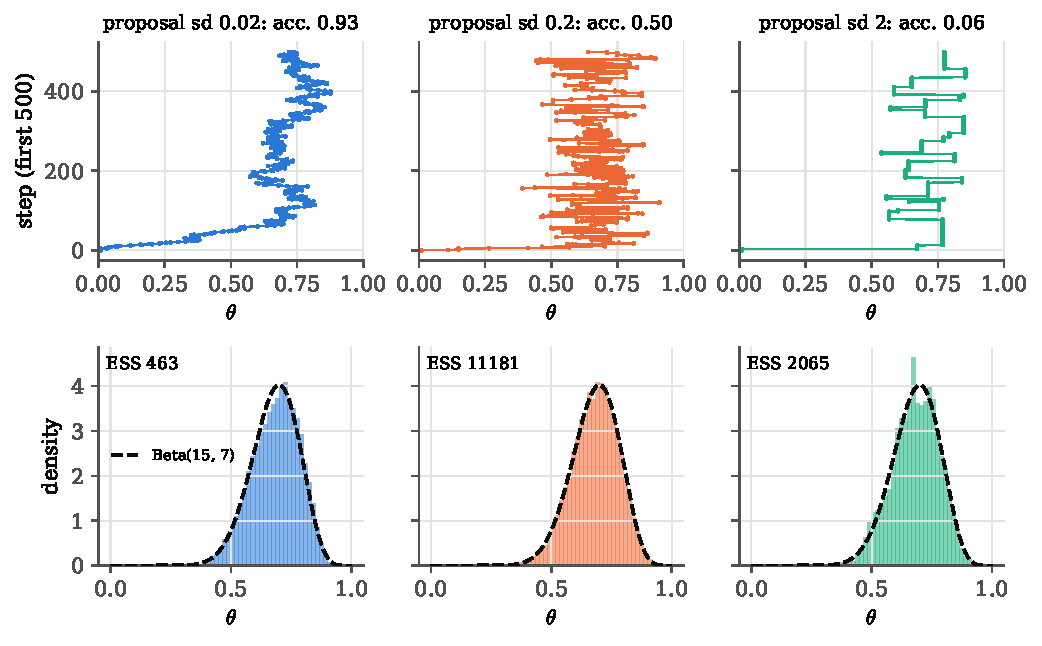
\includegraphics[width=\linewidth]{figures/ch09/coin_chains.pdf}
\caption{Kruschke's coin, reproduced. Top: the first 500 steps of three chains started at
$\theta=0.01$ with proposal widths 0.02, 0.2 and 2 (step number runs upwards). Bottom: histograms
of the remaining steps against the exact $\mathrm{Beta}(15,7)$ posterior, with the effective
sample size of each chain.}
\label{9b:fig:coin}
\end{figure}

All three coin histograms in \cref{9b:fig:coin} are close to the beta density. Every proposal
width gives the right answer eventually, because each defines a chain with the posterior as its
stationary distribution. What differs is how long ``eventually'' is, more than an order of magnitude
in effective sample size between the best and the worst width here.

\emph{The lesson.} The proposal width never decides whether the answer is right, only what it
costs; choosing it well is the subject of \cref{9b:sec:stepsize}.
\section{How big should the steps be?}
\label{9b:sec:stepsize}

Kruschke's three coin walkers of \cref{9b:sec:code} all converged to the same beta posterior, and
yet the best was worth more than ten times as many independent draws as the worst. The two bad
ones failed in opposite ways. The walker with tiny steps accepted almost everything but moved like
the drunkard, a distance $s\sqrt t$ in $t$ steps, so crossing a posterior of width $L$ took about
$(L/s)^2$ steps, the diffusive cost met at the end of \cref{9a:sec:diffusion}. The walker with
huge steps proposed points far out in the tails, refused them, and sat still for long stretches.
In between there must be a best step length, and since the target's width is usually unknown we
would like to recognise it from something the chain itself reports.

\paragraph{The question.} For a given target, which step length makes the walker produce
independent information fastest, and is there a quantity we can monitor, such as the fraction of
accepted proposals, that tells us we are there?

\subsection{The Gaussian in many dimensions: 2.38 and 0.234}
\label{9b:sec:0234}

The one target where this question has a clean answer is the standard Gaussian in $D$
dimensions, $f(x)\propto e^{-\abs x^2/2}$, sampled with round Gaussian steps
$y=x+(\ell/\sqrt D)\,z$, $z\sim\Normal(0,\Id_D)$, where $\ell$ is a dimensionless step scale.
Why divide by $\sqrt D$? Because the log ratio is a sum over all $D$ coordinates, and if each
coordinate moved by a fixed amount the sum would grow with $D$ and every proposal would be
refused. Shrinking the step per coordinate as $1/\sqrt D$ keeps the log ratio of order one.

\paragraph{The log ratio becomes Gaussian.}
For a walker at $x$ and a proposal $y=x+(\ell/\sqrt D)z$,
\begin{align}
  \ln R
  &\eqby{1}-\tfrac12\bigl(\abs{y}^2-\abs x^2\bigr)
   \eqby{2}-\frac{\ell}{\sqrt D}\,x\cdot z-\frac{\ell^2}{2D}\,\abs z^2
  \nonumber\\
  &\eqby{3}-\ell\,\frac{\abs x}{\sqrt D}\,\zeta-\frac{\ell^2}{2}\,\frac{\abs z^2}{D}
   \;\xrightarrow{D\to\infty}\;
   \Lambda\sim\Normal\Bigl(-\frac{\ell^2}2,\;\ell^2\Bigr).
  \label{9b:eq:logR-gauss}
\end{align}
\begin{explain}
  \item The normalisation of $f$ cancels; only the exponents differ.
  \item $\abs{x+v}^2=\abs x^2+2x\cdot v+\abs v^2$ with $v=(\ell/\sqrt D)z$.
  \item For fixed $x$, $x\cdot z$ is a sum of independent Gaussians with variance
        $\sum_ix_i^2=\abs x^2$, so $x\cdot z=\abs x\,\zeta$ with $\zeta\sim\Normal(0,1)$. A walker
        in equilibrium has $\abs x^2/D\to1$ and $\abs z^2/D\to1$ by the law of large numbers
        (both are averages of $D$ squared standard Gaussians), so the first term tends to
        $-\ell\zeta$ and the second to $-\ell^2/2$.
\end{explain}

\paragraph{The acceptance rate.}
Call the limiting log ratio of \eqref{9b:eq:logR-gauss} $\Lambda$ (a capital lambda, for
``log ratio''). The acceptance probability of one proposal is $\min(1,R)=\min(1,e^\Lambda)$, so
the mean acceptance is $a(\ell)=\E\bigl[\min(1,e^{\Lambda})\bigr]$ with
$\Lambda\sim\Normal(-\sigma^2/2,\sigma^2)$ and $\sigma=\ell$. Split it into the uphill part
($\Lambda>0$, accepted for sure) and the
downhill part:
\begin{align}
  a(\ell)
  &\eqby{1}\Prob(\Lambda>0)+\E\bigl[e^\Lambda;\,\Lambda<0\bigr]
  \nonumber\\
  &\eqby{2}\Phi\Bigl(-\frac\sigma2\Bigr)
   +\int_{-\infty}^0\frac{1}{\sigma\sqrt{2\pi}}\,
     \exp\Bigl[w-\frac{(w+\sigma^2/2)^2}{2\sigma^2}\Bigr]\dd w
  \nonumber\\
  &\eqby{3}\Phi\Bigl(-\frac\sigma2\Bigr)
   +\int_{-\infty}^0\frac{1}{\sigma\sqrt{2\pi}}\,
     \exp\Bigl[-\frac{(w-\sigma^2/2)^2}{2\sigma^2}\Bigr]\dd w
  \eqby{4}2\,\Phi\Bigl(-\frac\ell2\Bigr).
  \label{9b:eq:acc-theory}
\end{align}
\begin{explain}
  \item $\min(1,e^\Lambda)$ is $1$ when $\Lambda>0$ and $e^\Lambda$ when $\Lambda<0$; $\E[X;A]$ means the expectation of
        $X$ restricted to the event $A$.
  \item $\Prob(\Lambda>0)=\Prob\bigl(\sigma\zeta-\sigma^2/2>0\bigr)=\Prob(\zeta>\sigma/2)=\Phi(-\sigma/2)$,
        with $\Phi$ the standard Gaussian cumulative distribution; the second term is the
        Gaussian density of $\Lambda$ times $e^w$.
  \item Complete the square:
        $w-(w+\sigma^2/2)^2/2\sigma^2=-(w^2-\sigma^2w+\sigma^4/4)/2\sigma^2=-(w-\sigma^2/2)^2/2\sigma^2$.
        Multiplying by $e^w$ has moved the Gaussian's mean from $-\sigma^2/2$ to $+\sigma^2/2$.
  \item The integral is the probability that a $\Normal(\sigma^2/2,\sigma^2)$ variable is
        negative, which is again $\Phi(-\sigma/2)$; and $\sigma=\ell$.
\end{explain}
Small steps give $a\to2\Phi(0)=1$; large steps give $a\to0$. \Cref{9b:fig:step-scaling}a shows
that chains in $D=10$ and $50$ follow \eqref{9b:eq:acc-theory} closely, and that even $D=1$ is
not far from it.

\paragraph{The best step.}
\emph{How far does one step move the walker?} When a proposal is accepted, the walker moves by
$(\ell/\sqrt D)z$; when it is refused, by nothing. Write $A$ for the indicator of acceptance (1 if
taken, 0 if refused). The mean squared jump per step, summed over coordinates, is
\begin{align}
  \E\,\abs{x_{t+1}-x_t}^2
  &\eqby{1}\E\Bigl[\frac{\ell^2}{D}\,\abs z^2\,A\Bigr]
   \eqby{2}\ell^2\,\E\Bigl[\frac{\abs z^2}{D}\,A\Bigr]
   \relby{3}{\simeq}\ell^2\,\E[A]
   \eqby{4}\ell^2\,a(\ell)=2\ell^2\,\Phi(-\ell/2).
  \label{9b:eq:esjd}
\end{align}
\begin{explain}
  \item The squared jump is $\abs{(\ell/\sqrt D)z}^2=(\ell^2/D)\abs z^2$ if accepted and 0 if not.
  \item Take the constant $\ell^2$ out, leaving $\ell^2/D$ times $\abs z^2$ as $\ell^2$ times the
        average $\abs z^2/D$.
  \item $\abs z^2/D$ is an average of $D$ squared standard Gaussians, so for large $D$ it is 1
        with a spread of only $\sqrt{2/D}$; it is then a constant and comes out of the expectation.
        The acceptance $A$ depends on $z$ only through the one sum $x\cdot z$ of
        \eqref{9b:eq:logR-gauss} and through this same average, so no single $z_i$ matters and
        nothing correlates $A$ with the size of the jump.
  \item $\E[A]$ is the mean acceptance \eqref{9b:eq:acc-theory}.
\end{explain}

\emph{From jump size to autocorrelation time.} Follow one coordinate, $x_1$. Its share of the
mean squared jump is $\ell^2a(\ell)/D$ per step, and in equilibrium it spreads over a range of
standard deviation 1. A coordinate that moves by diffusion forgets where it was once it has
travelled about one standard deviation, and a diffusion with mean squared step $v$ needs about
$1/v$ steps for that, the cost $(L/s)^2$ of \cref{9a:sec:diffusion} with $L=1$ and $s^2=v$. So
\begin{equation*}
  \tau\;\propto\;\frac{D}{\ell^2\,a(\ell)} ,
\end{equation*}
and the step that maximises the mean squared jump minimises the autocorrelation time. The
statement that this is exact as $D\to\infty$ is the theorem of
\textcite{RobertsGelmanGilks1997}: watched on a clock that ticks $D$ steps at a time, each
coordinate of the chain becomes a diffusion (a Langevin process) whose speed is exactly
$h(\ell)=2\ell^2\Phi(-\ell/2)$.

\emph{Maximising the speed.} Set the derivative of $h$ to zero:
\begin{align*}
  0=\frac{\dd h}{\dd\ell}
  &\eqby{1}4\ell\,\Phi(-\ell/2)-\ell^2\,\phi(\ell/2)
  \quad\iff\quad
  4\,\Phi(-\ell/2)=\ell\,\phi(\ell/2),
\end{align*}
\begin{explain}
  \item Product rule, with $\dd\Phi(-\ell/2)/\dd\ell=-\tfrac12\phi(\ell/2)$ and $\phi$ the
        standard Gaussian density.
\end{explain}
whose root, found numerically, is $\ell=\NineBStLopt$. The acceptance there is
\begin{equation*}
  a=2\,\Phi\Bigl(-\frac{\NineBStLopt}{2}\Bigr)=2\,\Phi(-1.19)=2\times0.117=\NineBStAopt ,
\end{equation*}
so the best walker refuses $1-0.234\simeq\tfrac34$ of its proposals, three in four.

\emph{Why both extremes lose.} For small $\ell$ the acceptance tends to 1 and $h\approx\ell^2$
is small. For large $\ell$ the acceptance collapses, and the rate follows from the Gaussian tail.
For large $u$,
\begin{align*}
  \Phi(-u)
  &\eqby{1}\int_u^\infty\phi(t)\,\dd t
   \eqby{2}\phi(u)\int_u^\infty e^{-(t^2-u^2)/2}\,\dd t
   \eqby{3}\phi(u)\int_0^\infty e^{-u\,v-v^2/2}\,\dd v
   \;\approx\;\frac{\phi(u)}{u}=\frac{e^{-u^2/2}}{u\sqrt{2\pi}} .
\end{align*}
\begin{explain}
  \item $\Phi(-u)=\Prob(Z<-u)=\Prob(Z>u)$ for a standard Gaussian $Z$.
  \item $\phi(t)=\phi(u)\,e^{-(t^2-u^2)/2}$.
  \item Put $t=u+v$, so $t^2-u^2=2uv+v^2$. For large $u$ the factor $e^{-uv}$ cuts the integral
        off at $v\sim1/u$, where $v^2/2$ is negligible, and $\int_0^\infty e^{-uv}\dd v=1/u$.
\end{explain}
With $u=\ell/2$ this gives $a(\ell)=2\Phi(-\ell/2)\approx(4/\ell\sqrt{2\pi})\,e^{-\ell^2/8}$: the
acceptance dies like $e^{-\ell^2/8}$, faster than $\ell^2$ grows, and $h$ goes to zero. The
compromise between the two sits at $\ell=2.38$.

\begin{keyidea}[The 2.38 and 0.234 rule]
For a target that is roughly Gaussian in $D$ dimensions, the most efficient round random-walk
proposal has width $2.38/\sqrt D$ in units of the target's standard deviation, and accepts about
23\% of its proposals \parencite{RobertsGelmanGilks1997}. In one dimension the best acceptance is
higher, near one half. The chain then needs of order $D$ steps per independent draw
\srcref{HobsonBMC}{§3.2.4, p.~65}.
\end{keyidea}

\Cref{9b:fig:step-scaling}b measures the mean squared jump of real chains of $4\times10^4$ steps
on a grid of 22 step scales. The best measured acceptances are $\NineBStBestAccOne$ in $D=1$,
$\NineBStBestAccTen$ in $D=10$ and $\NineBStBestAccFifty$ in $D=50$, approaching $0.234$ as $D$
grows. At $\ell=2.38$ the integrated autocorrelation time of one coordinate, divided by $D$, is
$\NineBStTauDOne$, $\NineBStTauDTen$ and $\NineBStTauDFifty$: an independent draw every three
to four and a half times $D$ steps. \textcite{Dunkley2005} found the same for cosmological chains, an
inverse efficiency of about $3.3D$ and an optimal acceptance tending to 0.25, and recommended the
width $2.4/\sqrt D$ that \textcite{LewisBridle2002} use in CosmoMC. Wasserman's rule of thumb,
accept about half the proposals \mainref{p.~415}, is the one-dimensional answer; Kruschke's
adaptive phase aims at ``a middling value such as 0.5'' \srcref{Kruschke}{p.~161}. In many
dimensions the target is 0.2--0.3.

\begin{figure}[htbp]
\centering
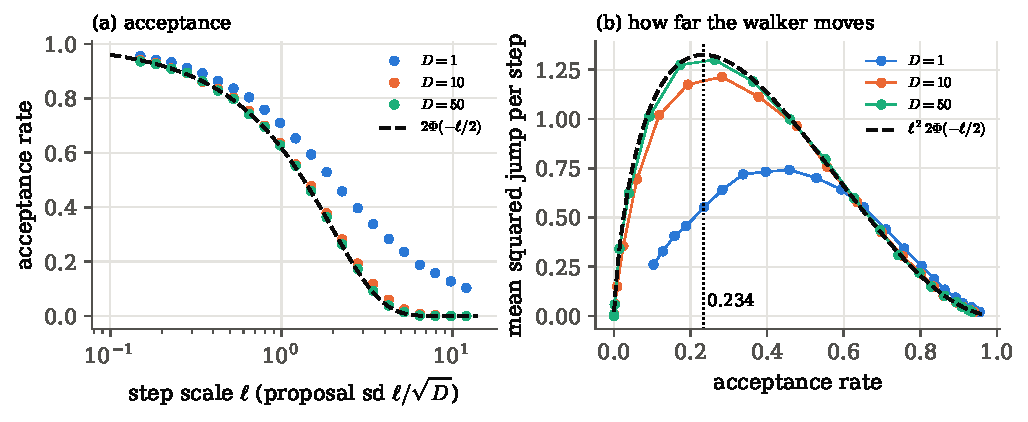
\includegraphics[width=\linewidth]{figures/ch09/step_scaling.pdf}
\caption{Step size on a standard Gaussian target in $D=1$, $10$ and $50$ dimensions, with
proposal width $\ell/\sqrt D$. (a) Measured acceptance against $\ell$, with the large-$D$
formula $2\Phi(-\ell/2)$ (dashed). (b) Mean squared jump per step against acceptance: it peaks
near acceptance 0.23 in many dimensions (dotted line), and near 0.45 in one dimension.}
\label{9b:fig:step-scaling}
\end{figure}

\subsection{Correlated targets: shape the steps like the posterior}
\label{9b:sec:shaped}

Real posteriors are rarely round. Two parameters that the data constrain only in combination,
such as the amplitude and tilt of a power spectrum, or the matter density and the Hubble rate,
give a long thin ellipse. Take the Gaussian with unit variances and correlation $\rho=0.95$,
covariance $\Cmat=\bigl(\begin{smallmatrix}1&\rho\\\rho&1\end{smallmatrix}\bigr)$. Its principal
axes are the eigenvectors of $\Cmat$:
\begin{align*}
  \det(\Cmat-\lambda\Id)
  &\eqby{1}(1-\lambda)^2-\rho^2=0
  \quad\iff\quad
  \lambda_\pm\eqby{2}1\pm\rho ,
\end{align*}
\begin{explain}
  \item Determinant of a $2\times2$ matrix.
  \item $1-\lambda=\mp\rho$; the eigenvectors are $(1,1)/\sqrt2$ for $1+\rho$ and $(1,-1)/\sqrt2$
        for $1-\rho$.
\end{explain}
The standard deviation along the ridge is $\sqrt{1.95}=1.40$ and across it
$\sqrt{0.05}=0.22$, a ratio of about six.

\emph{What a round step costs here.} A round step cannot be tuned to both widths at once.
Suppose we tune it to the narrow one, since that is the direction in which proposals are refused.
For a round Gaussian in $D=2$ the best step is $\ell/\sqrt D=2.38/\sqrt2\simeq1.7$ standard
deviations (\cref{9b:sec:0234}), so here it is about $1.7\times0.22\simeq0.37$. Along the ridge
the walker then diffuses with steps of that size, and by the diffusion cost $(L/s)^2$ of
\cref{9a:sec:diffusion} crossing a distance $L$ takes about $(L/s)^2$ steps:
\begin{align*}
  \text{ridge, step tuned to the narrow width:}\quad
  &\Bigl(\frac{1.40}{1.7\times0.22}\Bigr)^2\eqby{1}\Bigl(\frac{1.40}{0.37}\Bigr)^2\simeq14,
  \\
  \text{round target of width 1.40:}\quad
  &\Bigl(\frac{1.40}{1.7\times1.40}\Bigr)^2\eqby{2}\frac1{1.7^2}\simeq0.35,
  \\
  \text{ratio:}\quad
  &\eqby{3}\Bigl(\frac{1.40}{0.22}\Bigr)^2\simeq40 .
\end{align*}
\begin{explain}
  \item Ridge length $L=1.40$, step $s=1.7\times0.22$.
  \item For a round target the best step is 1.7 times its own width, so it crosses in less than
        one step.
  \item The factor 1.7 cancels: the penalty is the square of the ratio of the two widths.
\end{explain}
So a round step sized for the narrow direction makes the walker some forty times slower along the
ridge than the same walker on a round target. In practice the best round step is larger than
this, a compromise that accepts fewer proposals and moves farther along the ridge when it does,
and the penalty is smaller, as the runs below show; but no round step escapes it.

\Cref{9b:fig:step-correlated} shows four walkers of $4\times10^4$ steps on this ellipse. Tiny
round steps ($s=\NineBStCorrSmallStep$) are accepted $\NineBStCorrSmallAcc$ of the time and creep
along the ridge, with integrated autocorrelation time $\tau=\NineBStCorrSmallTau$ steps. Huge
round steps ($s=\NineBStCorrLargeStep$) are accepted a fraction $\NineBStCorrLargeAcc$ of the
time, $\tau=\NineBStCorrLargeTau$. The best round step of a scan, $s=\NineBStIsoBestStep$, gives
acceptance $\NineBStCorrTunedAcc$ and $\tau=\NineBStCorrTunedTau$. A proposal with the
covariance of the target itself, scaled by the 2.38 rule, gives acceptance
$\NineBStCorrShapedAcc$ and $\tau=\NineBStCorrShapedTau$.

\begin{figure}[htbp]
\centering
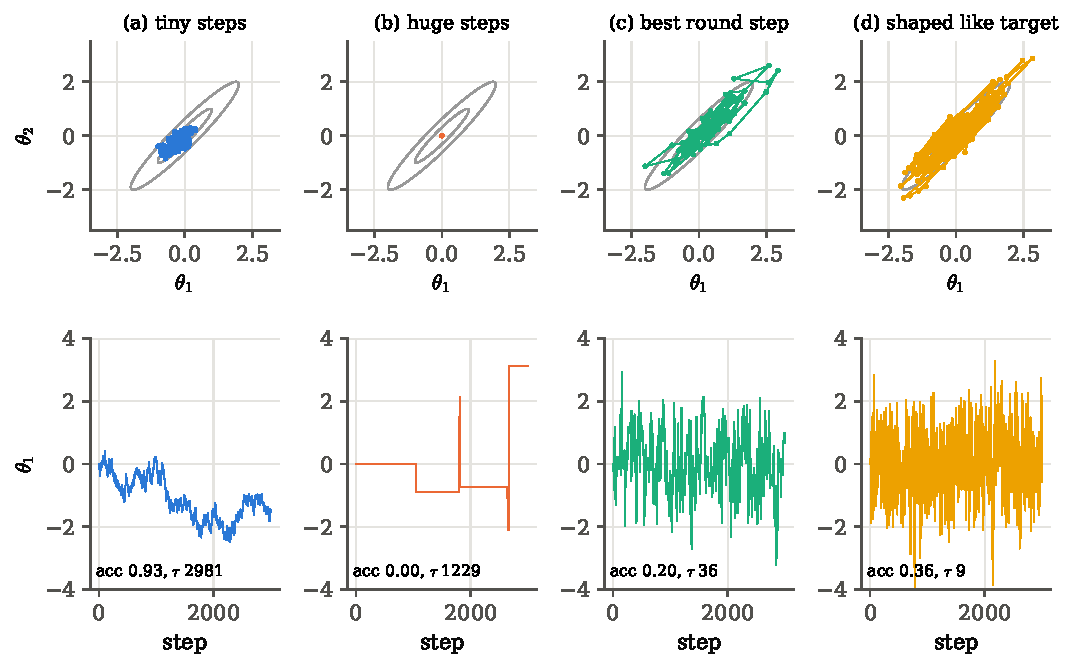
\includegraphics[width=\linewidth]{figures/ch09/step_correlated.pdf}
\caption{Four walkers on a Gaussian with correlation 0.95 (68\% and 95\% contours in grey).
Top: the first 400 steps. Bottom: 3000 steps of $\theta_1$, with acceptance rate and integrated
autocorrelation time. (a) Tiny round steps creep. (b) Huge round steps are almost always
refused. (c) The best round step still has to diffuse along the ridge. (d) Steps shaped like
the target cover it in a few moves.}
\label{9b:fig:step-correlated}
\end{figure}

Why does shaping work so well? Write the target's covariance as $\Cmat=LL\T$ (Cholesky) and
change to whitened coordinates $u=L^{-1}x$, in which the target is round. A shaped proposal
$y=x+sLz$ in the original coordinates is, in the new ones,
\begin{align*}
  u'
  &\eqby{1}L^{-1}y
   =L^{-1}x+sL^{-1}Lz
   \eqby{2}u+s\,z ,
\end{align*}
\begin{explain}
  \item Apply the linear map $L^{-1}$ to the proposal $y=x+sLz$.
  \item $L^{-1}x=u$ and $L^{-1}L=\Id$.
\end{explain}
a round proposal. And because the map is linear, its Jacobian is a constant that cancels from
every ratio. So the shaped walker on the ellipse \emph{is} the round walker on the round
Gaussian, and inherits its efficiency: with $\ell=2.38$ and $D=2$ the measured $\tau=\NineBStCorrShapedTau$ steps is a few
times $D$, whatever $\rho$ is. In practice the covariance is unknown, so one runs a short pilot chain,
estimates the covariance from it, and uses that for the proposal of the real run, repeating if
necessary \srcref{Padilla}{§4.1.4}, \srcref{HobsonBMC}{§3.2.4, p.~65}. The adaptation must stop
before the samples that are kept: a proposal that keeps changing with the chain's own history is
no longer a Markov chain with $f$ as its stationary law \srcref{HobsonBMC}{p.~63}.

\begin{pitfall}[A good acceptance rate is not a good chain]
The best round walker above accepted $\NineBStCorrTunedAcc$ of its proposals, right in the
recommended range, and was still several times slower than the shaped walker. The acceptance rate
measures only whether the step length suits the narrowest direction. It knows nothing about
whether the walker moves along the long ones. Judge a chain by its autocorrelation time or
effective sample size (\cref{9b:sec:diagnostics}), never by its acceptance rate alone.
\end{pitfall}

\subsection{Curved targets: change variables}
\label{9b:sec:banana}

A covariance matrix describes a straight ellipse. Many posteriors are curved, because the data
constrain a nonlinear combination of the parameters. The standard test case is the banana
\begin{equation}
  p(\theta_1,\theta_2)\propto\exp\Bigl[-\frac{\theta_1^2}{2}
    -\frac{(\theta_2-\theta_1^2)^2}{2\sigma^2}\Bigr],\qquad\sigma=\NineBBaSig .
  \label{9b:eq:banana}
\end{equation}
Read it as a recipe: $\theta_1\sim\Normal(0,1)$, and given $\theta_1$, $\theta_2$ is Gaussian with
mean $\theta_1^2$ and standard deviation $\sigma$. The exact moments follow from this reading:
\begin{align*}
  \E\theta_2
  &\eqby{1}\E\bigl[\E(\theta_2\given\theta_1)\bigr]=\E\theta_1^2=1,
  \\
  \Var\theta_2
  &\eqby{2}\Var\bigl(\E(\theta_2\given\theta_1)\bigr)+\E\bigl[\Var(\theta_2\given\theta_1)\bigr]
   =\Var(\theta_1^2)+\sigma^2
   \eqby{3}(3-1)+\sigma^2=2+\sigma^2,
  \\
  \Cov(\theta_1,\theta_2)
  &\eqby{4}\E\bigl[\theta_1\,\E(\theta_2\given\theta_1)\bigr]-\E\theta_1\,\E\theta_2
   =\E\theta_1^3=0 .
\end{align*}
\begin{explain}
  \item Tower rule: average the conditional mean over $\theta_1$.
  \item Law of total variance (\cref{ch:01}).
  \item $\E\theta_1^4=3$ and $\E\theta_1^2=1$ for a standard Gaussian.
  \item Odd moments of a standard Gaussian vanish.
\end{explain}
The last line is the trap: $\theta_1$ and $\theta_2$ are strongly dependent, yet their linear
correlation is exactly zero. A covariance matrix cannot see a symmetric banana.

\Cref{9b:fig:banana} confirms it with $\NineBBaN$ steps per walker. The best round walker has
$\tau=\NineBBaRoundTau$. A pilot run's covariance has correlation $\NineBBaPilotCorr$, which is
only noise, since the true correlation is zero. So the ``shaped'' proposal does little more than
rescale the two axes; it has acceptance
$\NineBBaShapedAcc$ and $\tau=\NineBBaShapedTau$. Both walkers struggle to get into the arms of
the banana. In this run their estimates of $\Var\theta_2$ are $\NineBBaRoundVarTwo$ and
$\NineBBaShapedVarTwo$, against the exact $\NineBBaVarTwoExact$. How much of that is luck? Run
each walker again $\NineBBaRepN$ times with fresh random numbers: the estimate moves by about
$\NineBBaRoundVarRepSd$ from run to run for the round walker and $\NineBBaShapedVarRepSd$ for the
shaped one. A slow chain sees only a few excursions into the arms, and the variance of a
long-tailed quantity depends on exactly those.

The cure is to remove the curvature by a change of variables. With $u=\theta_2-\theta_1^2$ the
target becomes $\exp[-\theta_1^2/2-u^2/2\sigma^2]$, a product of two independent Gaussians. The
map $(\theta_1,\theta_2)\mapsto(\theta_1,u)$ has Jacobian determinant
$\det\bigl(\begin{smallmatrix}1&0\\-2\theta_1&1\end{smallmatrix}\bigr)=1$, so no extra factor
appears in the density. A round walker in $(\theta_1,u)$, mapped back with
$\theta_2=u+\theta_1^2$, has acceptance $\NineBBaStraightAcc$, $\tau=\NineBBaStraightTau$, and
$\Var\theta_2=\NineBBaStraightVarTwo$, which moves by only $\NineBBaStraightVarRepSd$ from run to
run. Lewis and Bridle give the same advice for cosmology: when
a degeneracy is known, sample in the combination the data constrain well, for example the
angular size of the sound horizon instead of the Hubble rate, and remember the Jacobian in the
prior \srcref{HobsonBMC}{§3.2.4, p.~66}.

\begin{figure}[htbp]
\centering
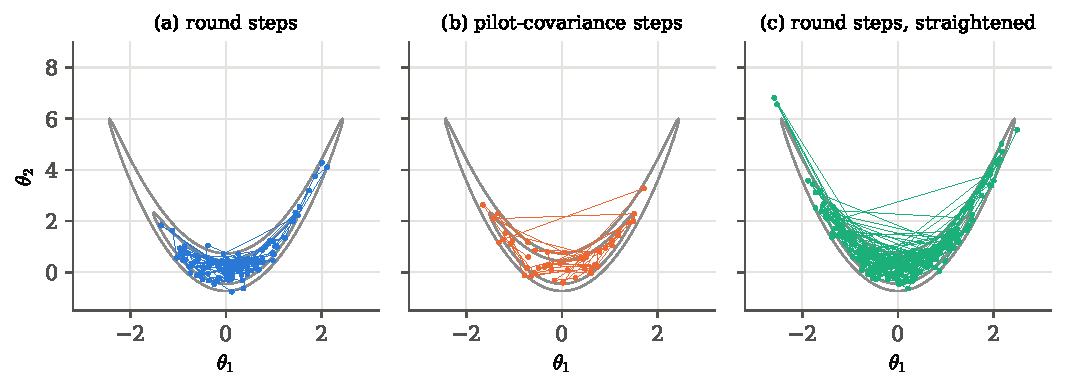
\includegraphics[width=\linewidth]{figures/ch09/banana_paths.pdf}
\caption{Six hundred steps of three walkers on the banana \eqref{9b:eq:banana}. (a) Round steps
and (b) steps shaped by a pilot covariance both crawl along the curved ridge. (c) Round steps
in the straightened variables $(\theta_1,\theta_2-\theta_1^2)$, mapped back, jump across the
whole banana.}
\label{9b:fig:banana}
\end{figure}

\paragraph{Cross-check against a standard library.}
The affine-invariant ensemble sampler \pyname{emcee} \parencite{ForemanMackey2013}, described
in \cref{9b:sec:relatives}, runs many walkers that propose moves along the lines joining them.
With $\NineBBaEmWalkers$ walkers and $\NineBBaEmSteps$ steps each on the banana it accepts
$\NineBBaEmAcc$ of its moves and reports an autocorrelation time of $\NineBBaEmTau$ steps, far
longer than the $\NineBBaStraightTau$ of the straightened walker: an affine-invariant method is
blind to linear correlations, but a banana is not linear. Its $\Var\theta_2$ is
$\NineBBaEmVarTwo$ in this run and moves by about $\NineBBaEmVarRepSd$ from run to run. The
triangle plot of \cref{9b:fig:banana-corner}, drawn with our own \pyname{corner} function,
overlays the straightened Metropolis chain and the \pyname{emcee} chain; the cores agree, and the
tips of the arms, where few samples land, are noisy in both.

\begin{figure}[htbp]
\centering
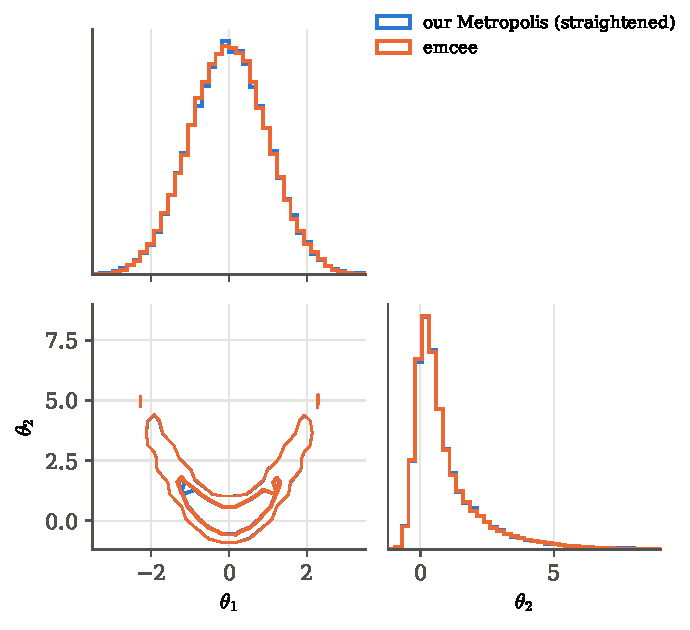
\includegraphics[width=0.62\linewidth]{figures/ch09/banana_corner.pdf}
\caption{Triangle plot of the banana: one-dimensional marginal histograms on the diagonal, 68\%
and 95\% regions of the two-dimensional histogram below it. Blue: our Metropolis sampler in the
straightened variables. Orange: \texttt{emcee} in the original variables.}
\label{9b:fig:banana-corner}
\end{figure}
\section{Reading a chain: burn-in, autocorrelation and effective sample size}
\label{9b:sec:diagnostics}

A finished run is a list of numbers, one row per step. Before quoting any average from it we have
to answer two questions \srcref{Kruschke}{§7.5}. Which part of the list is still remembering the arbitrary starting
point, and must be thrown away? And how much information is in the rest: how many independent
draws is it worth, and how accurate are the averages computed from it? The chain itself has to
answer both, because in a real problem nothing else knows the answer.

\subsection{Burn-in: where does equilibrium start?}
\label{9b:sec:burnin}

Start a Metropolis walker for the standard Gaussian in $D=\NineBAcDim$ dimensions at the point
$(10,10,\dots,10)$, ten standard deviations out in every coordinate, with the 2.38 step of
\cref{9b:sec:0234}. The quantity that shows the approach to equilibrium most clearly is the log
density along the chain, $\ln f(\theta_t)$, here $-\abs{\theta_t}^2/2$ up to a constant. It
starts at $\NineBAcLpStart$ and climbs (\cref{9b:fig:thin-burnin}b).

\paragraph{The question.} When has the walker arrived? The tempting answer, ``when it reaches
the peak'', is wrong, and seeing why is the most useful fact about high-dimensional posteriors.

In equilibrium $\theta\sim\Normal(0,\Id_D)$, so $\abs\theta^2=\sum_i\theta_i^2$ is a sum of $D$
squared standard Gaussians, a $\chi^2_D$ variable (\cref{ch:02}). Therefore
\begin{align}
  \E\bigl[\ln f(\theta)\bigr]
  &\eqby{1}-\tfrac12\E\chi^2_D=-\frac D2,
  \qquad
  \mathrm{sd}\bigl[\ln f(\theta)\bigr]
  \eqby{2}\tfrac12\sqrt{\Var\chi^2_D}=\tfrac12\sqrt{2D}=\sqrt{D/2}.
  \label{9b:eq:lnp-typical}
\end{align}
\begin{explain}
  \item $\E\theta_i^2=1$ for each of the $D$ terms.
  \item $\Var\theta_i^2=\E\theta_i^4-1=3-1=2$, and the $D$ terms are independent.
\end{explain}
For $D=10$ the equilibrium walker lives at $\ln f=-5\pm2.2$, never at the peak value 0. The
chain agrees: after step 10\,000 its $\ln f$ averages $\NineBAcLpEqMean$ with standard deviation
$\NineBAcLpEqSd$, and the highest value it ever reached was $\NineBAcLpMax$.

\emph{Why the walker avoids the peak.} The reason is volume. Ask how probable it is to find the
walker at a distance between $r$ and $r+\dd r$ from the centre. The density there is the same at
every point, $e^{-r^2/2}$ up to a constant, and the points form a thin spherical shell whose volume
is its area times its thickness. The area of a sphere of radius $r$ in $D$ dimensions grows as
$r^{D-1}$ (a circle's length as $r$, a sphere's area as $r^2$, and so on). So the radius has the
density
\begin{align}
  p(r)
  &\eqby{1}(\text{area}\propto r^{D-1})\times(\text{density } e^{-r^2/2})
   \propto r^{D-1}e^{-r^2/2},
  \nonumber\\
  \frac{\dd\ln p}{\dd r}
  &\eqby{2}\frac{D-1}{r}-r=0
   \quad\Longrightarrow\quad
   r_{\rm peak}^2\eqby{3}D-1\approx D .
  \label{9b:eq:shell}
\end{align}
\begin{explain}
  \item Probability in a thin shell is density times shell volume, and the shell volume is
        area times $\dd r$.
  \item $\ln p=(D-1)\ln r-r^2/2+\text{const}$; set its derivative to zero to find the most
        probable radius.
  \item Multiply by $r$ and solve.
\end{explain}
The first factor is zero at the centre and grows; the second is largest at the centre and dies
quickly; their product peaks at $r\approx\sqrt D$. At that radius $\ln f=-r^2/2\approx-D/2$, the
equilibrium mean of \eqref{9b:eq:lnp-typical}. For $D=10$ the most probable radius is
$\sqrt9=3$, where $\ln f=-4.5$, against the chain's average $\NineBAcLpEqMean$; the peak of $f$ at
$r=0$ has no volume around it at all. The bulk of the probability sits on a thin shell away from
the mode. Lambert calls this region the \newterm{typical set}, and describes
MCMC as two phases, first finding the typical set and then exploring it
\srcref{Lambert}{§13.7.1}.

Burn-in therefore ends when $\ln f$ stops climbing and starts fluctuating around a steady level,
not when it reaches the maximum. Here the trace first crossed its equilibrium median at step
$\NineBAcBurn$ (\cref{9b:fig:thin-burnin}b). A popular rule in cosmology discards the start of a
chain while $p/p_{\max}<0.1$ \parencite{Dunkley2005}. Read literally with the true peak, it must
be scaled with dimension. For a Gaussian posterior, $-2\ln(p/p_{\max})$ is exactly the
$\abs\theta^2$ above, a $\chi^2_D$ variable, so the fraction of equilibrium draws that satisfy
$p/p_{\max}\ge0.1$ is $\Prob(\chi^2_D\le2\ln10)$: $\NineBMcNearPeakTwo$ for $D=2$,
$\NineBMcNearPeakTen$ for $D=10$, and $\NineBMcNearPeakFifty$ for $D=50$. In fifty dimensions an
equilibrium chain essentially never comes within a factor of ten of the peak. Any threshold on
$\ln p$ has to be judged against the spread \eqref{9b:eq:lnp-typical} of $\ln p$ in equilibrium.
Two practical rules are common: look at the trace of $\ln p$ and of each parameter and cut where
they become stationary; or, with several chains, discard the first half of each by default
\srcref{Lambert}{§13.9.5}, \srcref{Kruschke}{§7.5.1}. Multiple chains make the cut checkable
(\cref{9b:sec:rhat}).

\begin{figure}[htbp]
\centering
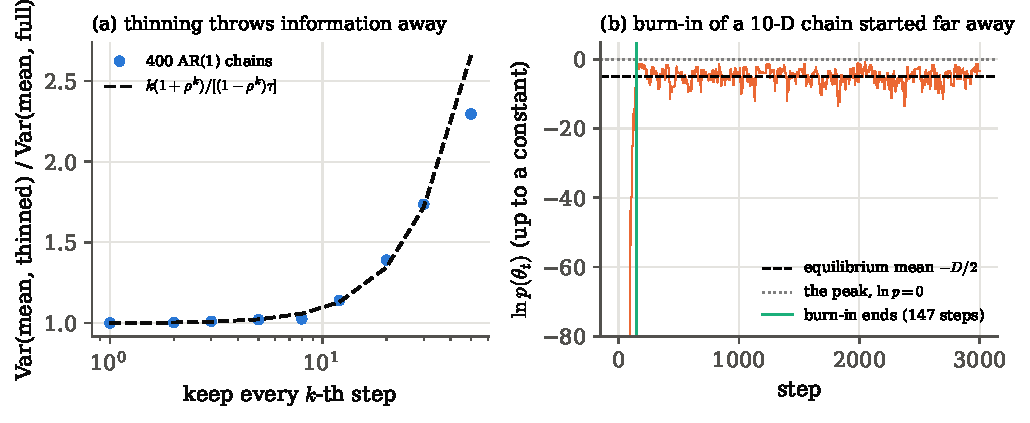
\includegraphics[width=\linewidth]{figures/ch09/thin_burnin.pdf}
\caption{(a) Thinning an AR(1) chain with $\rho=0.9$ by keeping every $k$th step: the variance of
the mean of the thinned chain, relative to the full chain, measured over 400 chains (dots) and
predicted (dashed). It is never below one. (b) $\ln p$ along a 10-dimensional chain started far
out: it climbs from $-500$ and settles around $-D/2$ (dashed), well below the peak value 0
(dotted).}
\label{9b:fig:thin-burnin}
\end{figure}

\subsection{Autocorrelation and the integrated autocorrelation time}
\label{9b:sec:tau}

Once the burn-in is gone, the remaining $N$ steps $x_1,\dots,x_N$ of one parameter are a
stationary but correlated series: every $x_t$ has the same variance $\sigma^2$, and the covariance
$C_k=\Cov(x_t,x_{t+k})=\sigma^2\rho_k$ depends only on the lag $k$, with $\rho_k$ the
autocorrelation. How accurate is the chain average $\bar x=\frac1N\sum_tx_t$? The derivation of
\cref{9a:sec:time-average-variance}, repeated in three lines:
\begin{align}
  \Var(\bar x)
  &\eqby{1}\frac1{N^2}\sum_{s=1}^N\sum_{t=1}^NC_{\abs{t-s}}
   \eqby{2}\frac{\sigma^2}{N}\Bigl[1+2\sum_{k=1}^{N-1}\Bigl(1-\frac kN\Bigr)\rho_k\Bigr]
   \eqby{3}\frac{\sigma^2}{N}\,\tau,
  \qquad
  \tau=1+2\sum_{k=1}^\infty\rho_k .
  \label{9b:eq:var-mean-recall}
\end{align}
\begin{explain}
  \item The variance of a sum is the sum of all the covariances of its terms.
  \item The $N$ pairs with $s=t$ give $N\sigma^2$; the $2(N-k)$ ordered pairs at lag $k\ge1$ give
        $2(N-k)\sigma^2\rho_k$; divide by $N^2$.
  \item For $N$ much longer than the range of the correlations, $k/N$ is negligible wherever
        $\rho_k$ is not, and the sum can run to infinity.
\end{explain}
With independent draws $\tau=1$ and this is the familiar $\sigma^2/N$; correlation replaces $N$ by
$N/\tau$, so the chain is worth $N/\tau$ independent draws. In \cref{9a:sec:ergodic} we computed
$\tau$ exactly from the transition matrix; now we must estimate it from the series alone.

\paragraph{Estimating the autocorrelation.}
The natural estimator of the lag-$k$ covariance averages the products of deviations $k$ steps
apart,
\begin{equation}
  \hat C_k=\frac1N\sum_{t=1}^{N-k}(x_t-\bar x)(x_{t+k}-\bar x),
  \qquad
  \hat\rho_k=\hat C_k/\hat C_0 ,
  \label{9b:eq:acf-hat}
\end{equation}
the \newterm{autocorrelation function} (ACF) of the chain \srcref{Kruschke}{§7.5.2}. It is
computed for all lags at once with a fast Fourier transform (\pyname{acf} in
\pyname{lib_mcmc.py}). One might now plug every $\hat\rho_k$ into \eqref{9b:eq:var-mean-recall}.
That gives exactly zero, for any data:
\begin{align}
  N\Bigl[\hat C_0+2\sum_{k=1}^{N-1}\hat C_k\Bigr]
  &\eqby{1}\sum_{s=1}^N\sum_{t=1}^N(x_s-\bar x)(x_t-\bar x)
   \eqby{2}\Bigl[\sum_{t=1}^N(x_t-\bar x)\Bigr]^2
   \eqby{3}0 .
  \label{9b:eq:naive-tau}
\end{align}
\begin{explain}
  \item Group the $N^2$ ordered pairs $(s,t)$ by their lag $\abs{t-s}=k$: lag 0 gives $N\hat
        C_0$ and each lag $k\ge1$ appears twice, giving $2N\hat C_k$.
  \item A double sum of products of the same terms is the square of the single sum.
  \item Deviations from the sample mean sum to zero.
\end{explain}
So $1+2\sum_{k\ge1}\hat\rho_k=0$ identically; our script finds it to be zero to within
$\NineBAcNaiveMax$, rounding error. The estimated autocorrelations at large lags are almost pure
noise, and they are forced to cancel the real correlation at small lags. The sum must be cut off
at a window $M$ beyond which the true $\rho_k$ is negligible but the noise is not yet large.

\paragraph{Choosing the window.}
Kruschke stops the sum at the first lag with $\hat\rho_k<0.05$ \srcref{Kruschke}{eq.~7.11}.
Stan, following Geyer, stops when the sum of two consecutive estimates first turns negative
\srcref{Lambert}{§13.10}. Our library uses Sokal's self-consistent window: the smallest $M$ with
$M\ge c\,\hat\tau(M)$, where $\hat\tau(M)=1+2\sum_{k=1}^M\hat\rho_k$ and $c\simeq5$
\parencite{Sokal1997}. The window then grows with the correlation time itself, so that slowly
decaying correlations are not cut short.

\emph{Why the window scales with $\tau$, and why $c\simeq5$.} Cutting the sum at $M$ makes two
errors that pull in opposite directions. The first is the correlation left out. If the true
autocorrelation decays as $\rho_k\simeq e^{-k/T}$ over some number of steps $T$, the sum gives
$\tau\simeq2T$ and the omitted tail is $2\sum_{k>M}e^{-k/T}\simeq2T\,e^{-M/T}$, a fraction
$e^{-M/T}$ of $\tau$. The second is noise. Each $\hat\rho_k$ fluctuates by about $1/\sqrt N$ (a
little more for a correlated series), and adding $M$ of them adds noise that grows like
$\sqrt M$; the careful calculation \parencite{Sokal1997} gives
\begin{equation}
  \frac{\Var(\hat\tau)}{\tau^2}\simeq\frac{2(2M+1)}{N}.
  \label{9b:eq:tau-noise}
\end{equation}
The omitted part shrinks exponentially in $M/T$, the noise grows only like $\sqrt M$, so the
right window is a few times the correlation length, and since $T$ is not known the estimate
$\hat\tau$ itself is used as the ruler: $M=c\hat\tau$. With $c=5$ the omitted fraction is
$e^{-10}$ for a single exponential and stays below $e^{-5}\simeq0.7\%$ even if a slow component
makes $T$ as long as $\tau$, while the relative noise is $\sqrt{2(10\tau+1)/N}$, still small once
$N$ is a few hundred times $\tau$. For the AR(1) test below, $\tau=19$ and $N=10^4$ give
$M\simeq95$ and a predicted spread of $\sqrt{191\times2/10^4}\times19\simeq3.7$ in $\hat\tau$.

\pyfile[firstline=91,lastline=98]{code/ch09/lib_mcmc.py}{Integrated autocorrelation time with
Sokal's window}

\paragraph{Example: calibrating on a chain with known $\tau$.}
The AR(1) chain $x_{t+1}=\rho x_t+\sqrt{1-\rho^2}\,z_t$ of \cref{9a:sec:ar1-forgetting} has
$\rho_k=\rho^k$ exactly, so
\begin{equation*}
  \tau=1+2\sum_{k\ge1}\rho^k=1+\frac{2\rho}{1-\rho}=\frac{1+\rho}{1-\rho},
\end{equation*}
which is $\NineBAcTauExact$ for $\rho=\NineBAcRho$. Over $\NineBAcR$ chains of $\NineBAcN$ steps,
Kruschke's rule gives $\hat\tau=\NineBAcKrMean\pm\NineBAcKrSd$ (mean and spread over the
chains), slightly low because it drops the tail of the correlation; Sokal's window gives
$\NineBAcSoMean\pm\NineBAcSoSd$, unbiased but noisier (\cref{9b:fig:acf}a), with a spread close
to the $3.7$ that \eqref{9b:eq:tau-noise} predicts. The prediction
\eqref{9b:eq:var-mean-recall} itself checks out: across the same kind of chains,
$N\Var(\bar x)/\sigma^2=\NineBAcVarMeanMeas$ against $\tau=\NineBAcVarMeanPred$. As a cross-check
against a standard library, \pyname{emcee}'s estimator \pyname{integrated_time}, applied to a
Metropolis chain of $2\times10^5$ steps on a standard Gaussian, returns $\tau=\NineBMcTauEmcee$,
and ours returns $\NineBMcTauOurs$.

\begin{workdef}[effective sample size and Monte Carlo standard error]
For a chain of $N$ steps of one quantity with integrated autocorrelation time $\tau$, the
\newterm{effective sample size} is
\begin{equation*}
  \mathrm{ESS}=\frac{N}{\tau}=\frac{N}{1+2\sum_{k\ge1}\rho_k}
\end{equation*}
\unpack{the number of independent draws that would give the mean with the same accuracy}
\srcref{Kruschke}{eq.~7.11}, \srcref{Lambert}{§13.10}, and the \newterm{Monte Carlo standard
error} of the chain average is
$\mathrm{MCSE}=\mathrm{SD}/\sqrt{\mathrm{ESS}}=\mathrm{SD}\sqrt{\tau/N}$
\srcref{Kruschke}{eq.~7.12}, with SD the standard deviation of the chain.
\emph{Operational recipe:} discard the burn-in, estimate $\tau$ with a window
(\pyname{tau_int}), and quote $\mathrm{ESS}$ for every parameter; the smallest one counts.
\end{workdef}

Note the difference between the two numbers in the box. The MCSE is the error of our
\emph{computation} of the posterior mean, the error that a longer run would reduce. The SD is the
width of the posterior itself, the uncertainty about the parameter that no amount of computing
removes. A run is long enough when the first is small compared with the second.

\paragraph{Example: Kruschke's coin chains.}
\Cref{9b:fig:acf}b shows the ACFs of the three coin chains of \cref{9b:sec:code}. With proposal
width 0.02 the ACF is still high after 60 steps; with width 2 it decays slowly too, because the
chain repeats the same value for long stretches; with width 0.2 it falls to near zero within ten
lags. These shapes are why the three effective sizes differed so much. For the middle chain,
$\mathrm{ESS}\approx\NineBCoinEssMid$ and the posterior SD is about $0.1$, so the posterior mean
is computed to $\mathrm{MCSE}\approx0.1/\sqrt{\NineBCoinEssMid}\approx0.001$, far below the SD.
Kruschke recommends an ESS of about 10\,000 when the limits of a 95\% interval are wanted, since
tails are sampled more sparsely than the centre \srcref{Kruschke}{§7.5.2}.

\begin{figure}[htbp]
\centering
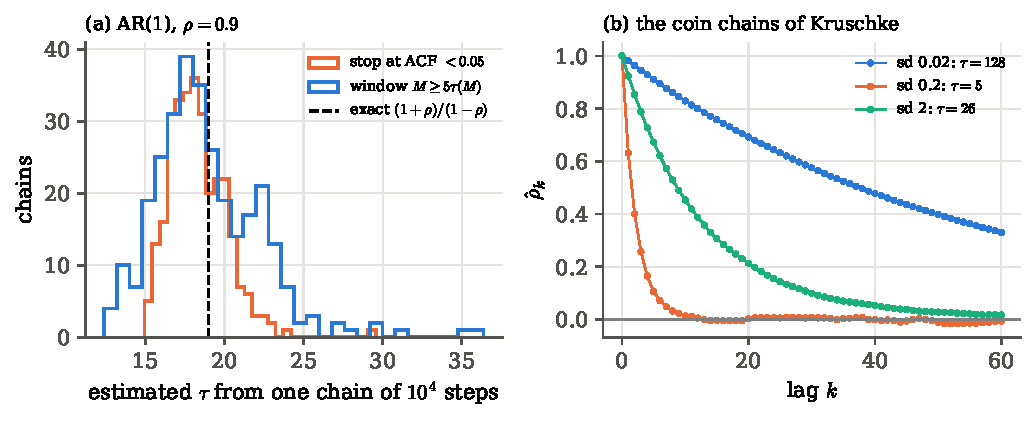
\includegraphics[width=\linewidth]{figures/ch09/acf_tau.pdf}
\caption{(a) Estimates of $\tau$ from single AR(1) chains of $10^4$ steps with exact $\tau=19$
(dashed): stopping at the first $\hat\rho_k<0.05$ is slightly biased low, Sokal's
self-consistent window is centred on the truth. (b) Autocorrelation functions of Kruschke's three
coin chains, with their estimated $\tau$.}
\label{9b:fig:acf}
\end{figure}

\subsection{Thinning}
\label{9b:sec:thinning}

Keeping only every $k$th step makes the stored points look less correlated, and is often done.
Does it make the averages better? For the AR(1) chain $x_{t+1}=\rho x_t+\sqrt{1-\rho^2}\,z_t$
(\cref{9b:sec:tau}, with $z_t$ independent standard Gaussians) the answer can be computed exactly.

\emph{The thinned chain is again AR(1).} Apply the recursion $k$ times:
\begin{align*}
  x_{t+k}
  &\eqby{1}\rho^k x_t+\sqrt{1-\rho^2}\sum_{j=0}^{k-1}\rho^j z_{t+k-1-j},
  \\
  \Var\Bigl(\sqrt{1-\rho^2}\sum_{j=0}^{k-1}\rho^j z_{t+k-1-j}\Bigr)
  &\eqby{2}(1-\rho^2)\frac{1-\rho^{2k}}{1-\rho^2}=1-\rho^{2k}.
\end{align*}
\begin{explain}
  \item Substitute $x_{t+k-1}=\rho x_{t+k-2}+\dots$ into itself $k$ times; each earlier kick
        arrives multiplied by one more factor $\rho$.
  \item The kicks are independent with variance 1, so the variances add:
        $(1-\rho^2)\sum_{j=0}^{k-1}\rho^{2j}$, a geometric sum.
\end{explain}
So the kept points obey $x_{t+k}=\rho^kx_t+\sqrt{1-\rho^{2k}}\,z'$ with a fresh standard Gaussian
$z'$, built from kicks that no other kept step uses: the same AR(1) form with coefficient
$\rho^k$. Its stationary variance is still $\sigma^2=1$, as it must be, since every $x_t$ in
equilibrium has the same distribution whichever steps we keep. The thinned chain has $N/k$
points. By \eqref{9b:eq:var-mean-recall} with the AR(1) $\tau$,
\begin{align}
  \frac{\Var(\bar x_{\rm thinned})}{\Var(\bar x_{\rm full})}
  &\eqby{1}\frac{\dfrac{\sigma^2k}{N}\,\dfrac{1+\rho^k}{1-\rho^k}}
            {\dfrac{\sigma^2}{N}\,\dfrac{1+\rho}{1-\rho}}
   \eqby{2}\frac{k\coth(ka/2)}{\coth(a/2)}
   \relby{3}{\ge}1,
   \qquad \rho=e^{-a}.
  \label{9b:eq:thinning}
\end{align}
\begin{explain}
  \item Numerator: $N/k$ points with correlation time $(1+\rho^k)/(1-\rho^k)$. Denominator: $N$
        points with $\tau=(1+\rho)/(1-\rho)$.
  \item $(1+e^{-b})/(1-e^{-b})=\coth(b/2)$, used with $b=ka$ and $b=a$.
  \item The function $u\coth u$ increases for $u>0$: its derivative is
        $\coth u-u/\sinh^2u=(\tfrac12\sinh2u-u)/\sinh^2u>0$, because $\sinh v>v$ for $v>0$. Hence
        $(ka/2)\coth(ka/2)\ge(a/2)\coth(a/2)$ for $k\ge1$; multiply by $2/a$.
\end{explain}
Thinning never helps the average; it can only lose information. For $\rho=0.9$ and $k=20$ the
predicted ratio is $\NineBAcThinTwenty$ and 400 simulated chains give $\NineBAcThinTwentyMeas$
(\cref{9b:fig:thin-burnin}a). The variance grows by a third although only one point in twenty
was kept; when the steps are strongly correlated the discarded ones carried little, but never
nothing.

\begin{pitfall}[Thinning is for storage, not accuracy]
Thinning a chain does not make it ``more independent'' in any useful sense: the thinned average
is never more accurate than the full one \eqref{9b:eq:thinning}. Thin only to save memory or
disk, for example when each step stores a whole map \srcref{Lambert}{§13.10.1},
\srcref{Padilla}{§4.1.4}, and report the ESS of what you kept.
\end{pitfall}
\section{Many chains from far apart: the Gelman--Rubin statistic}
\label{9b:sec:rhat}

A single chain can look perfectly healthy and be wrong. If the posterior has a second region of
high probability that the walker never found, the trace is stationary, the ACF decays, the ESS is
large, and every number in \cref{9b:sec:diagnostics} is computed from the wrong distribution.
Nothing inside one chain can reveal a region the chain has never visited. The remedy is to send
out several walkers from starting points spread far wider than the posterior is expected to be,
and to see whether they end up telling the same story \srcref{Padilla}{§4.1.3},
\srcref{Kruschke}{§7.5.1}.

\paragraph{The question.} This was the question \textcite{GelmanRubin1992} set out to answer:
given $M$ chains of $N$ steps each, started far apart, how can we tell from the chains alone that
none of them still remembers where it started? Put differently, how do we turn ``they agree''
into a number, and how close to its ideal value must the number be?

\paragraph{Example: four walkers on the two bumps.}
Take again the two-bump density \eqref{9b:eq:two-bumps}, with bumps at $x=-2$ and $x=+2$, and
start four Metropolis walkers (step 1.5) at $x_0=-30$, $-10$, $+10$ and $+30$, ten to fifteen
posterior widths away. \Cref{9b:fig:multichain}a shows that within a hundred steps all four have
fallen into the region of the bumps and are hopping between them. The histograms of the second
halves of the four chains, $\NineBMcN$ steps each, lie on top of one another and of $f$
(\cref{9b:fig:multichain}b). Their four means range from $\NineBMcMeanLo$ to $\NineBMcMeanHi$,
around the exact $\NineBMcMeanExact$.

\paragraph{Within and between.}
Index the chains by $j=1,\dots,M$ and the steps by $i=1,\dots,N$, so $\theta_{ij}$ is step $i$ of
chain $j$; let $\bar\theta_j$ be the mean of chain $j$ and $\bar\theta$ the mean of everything.
Two quantities summarise the spread \srcref{Padilla}{eqs.~57--60}, \srcref{Lambert}{§13.9.3}:
\begin{equation}
  W=\frac1M\sum_{j=1}^M s_j^2,\quad s_j^2=\frac{1}{N-1}\sum_{i=1}^N(\theta_{ij}-\bar\theta_j)^2,
  \qquad
  \frac BN=\frac{1}{M-1}\sum_{j=1}^M(\bar\theta_j-\bar\theta)^2 .
  \label{9b:eq:WB}
\end{equation}
$W$ is the average variance \emph{within} a chain. $B/N$ is the variance \emph{between} the chain
means. The sources write these with slightly different letters:
\begin{center}
\begin{tabular}{lccc}
\toprule
 & here & \textcite{GelmanRubin1992}, Lambert & Padilla, eq.~59\\
\midrule
variance of the chain means & $B/N$ & $B/N$ (their $B$ is $N$ times it) & $B$\\
average within-chain variance & $W$ & $W$ & $W$\\
\bottomrule
\end{tabular}
\end{center}
Gelman and Rubin multiply the variance of the means by $N$ so that their $B$ is comparable with
the variance of single draws; we keep their $B$ and always write it as $B/N$. If the chains have not
mixed, each one has explored only part of the posterior: $W$ is too small, because no chain has
seen the full spread, and $B/N$ is too large, because the chains sit in different places.

How are $W$ and $B/N$ related when the chains \emph{are} all in equilibrium? Write $\sigma^2$ for
the posterior variance and $v=\Var(\bar\theta_j)$ for the variance of a chain mean, which by
\eqref{9b:eq:var-mean-recall} is $\sigma^2\tau/N$. Then
\begin{align}
  \E\Bigl[\frac{N-1}{N}\,W\Bigr]
  &\eqby{1}\E\Bigl[\frac1N\sum_{i=1}^N(\theta_{ij}-\bar\theta_j)^2\Bigr]
   \eqby{2}\E\Bigl[\frac1N\sum_{i}(\theta_{ij}-\mu)^2\Bigr]-\E(\bar\theta_j-\mu)^2
   \eqby{3}\sigma^2-v,
  \nonumber\\
  \E\Bigl[\frac BN\Bigr]
  &\eqby{4}v,
  \qquad\text{so}\qquad
  \E\Bigl[\frac{N-1}{N}\,W+\frac BN\Bigr]=\sigma^2 .
  \label{9b:eq:sigma-plus}
\end{align}
\begin{explain}
  \item Definition of $s_j^2$; all chains have the same expectation.
  \item With $\mu$ the posterior mean,
        $\sum_i(\theta_{ij}-\bar\theta_j)^2=\sum_i(\theta_{ij}-\mu)^2-N(\bar\theta_j-\mu)^2$,
        the parallel-axis theorem for the sum of squares.
  \item Each $\theta_{ij}$ has variance $\sigma^2$; $\E(\bar\theta_j-\mu)^2=v$. This holds for
        correlated draws as well: correlation only changes $v$ from $\sigma^2/N$
        to $\sigma^2\tau/N$.
  \item Independent chains: the chain means are $M$ independent draws with variance $v$, and
        \eqref{9b:eq:WB} is their unbiased sample variance.
\end{explain}
So the pooled estimate $\hat\sigma^2_+=\frac{N-1}NW+\frac BN$ is unbiased for the posterior
variance once the chains are in equilibrium. From here Gelman and Rubin's statistic follows in
three moves.

\emph{Before equilibrium, the two estimates err in opposite directions.} Started overdispersed,
the chain means are spread not only by the noise $v$ of \eqref{9b:eq:sigma-plus} but also by the
memory of their starting points, which were chosen wider than the posterior. That extra spread
enters $B/N$, so $\hat\sigma^2_+$ is too \emph{large}. At the same time each chain has explored
only the part of the posterior near where it is, and the sample variance $s_j^2$ of a chain that
has not yet seen the whole posterior is too \emph{small}; so is their average $W$. The true
$\sigma^2$ lies between the two:
\begin{equation*}
  \E W\;\lesssim\;\sigma^2\;\lesssim\;\E\hat\sigma^2_+ ,
\end{equation*}
and both inequalities become equalities as the chains forget their starts.

\emph{The uncertainty of the centre.} The pooled estimate describes the spread of draws around
the true posterior mean $\mu$. But $\mu$ is not known; it is estimated by the grand mean
$\bar\theta$, the average of $M$ chain means, each with variance $B/N$. Its variance is therefore
$B/(MN)$, and the spread of a draw around the \emph{estimated} centre is
\begin{align*}
  \hat V
  &\eqby{1}\hat\sigma^2_+ +\frac{B}{MN}
   \eqby{2}\frac{N-1}{N}\,W+\Bigl(1+\frac1M\Bigr)\frac BN .
\end{align*}
\begin{explain}
  \item The variance of a draw around $\bar\theta$ is the variance around $\mu$ plus the variance
        of $\bar\theta$ itself: variances of independent pieces add, and one draw out of $MN$
        barely moves $\bar\theta$, so the two are very nearly independent.
  \item Collect the two terms in $B/N$.
\end{explain}
With few chains the centre is poorly known and the correction matters: for $M=4$ it adds a
quarter to the between-chain term.

\emph{The ratio, in units of a standard deviation.} $\hat V$ errs high and $W$ errs low, so
$\hat V/W$ is above 1 while the chains still remember their starts and tends to 1 as they mix.
Its square root compares two standard deviations instead of two variances: it is the factor by
which the present estimate of the posterior's \emph{scale} could still shrink if the chains ran
forever, hence the name \parencite{GelmanRubin1992}.

\begin{workdef}[potential scale reduction factor $\hat R$]
For $M$ chains of $N$ post-burn-in steps of one parameter, with $W$ and $B/N$ as in
\eqref{9b:eq:WB},
\begin{equation}
  \hat V=\frac{N-1}{N}\,W+\Bigl(1+\frac1M\Bigr)\frac BN,
  \qquad
  \hat R=\sqrt{\hat V/W}
  \label{9b:eq:rhat}
\end{equation}
\unpack{by how much the estimated posterior spread could still shrink if the chains ran forever}.
$\hat R\to1$ from above as the chains mix. \emph{Operational test:} compute $\hat R$ for every
parameter, on the second halves of the chains, and keep running until all are below a threshold.
Kruschke worries above 1.1 \srcref{Kruschke}{§7.5.1}; current practice often asks for 1.01.
Splitting every chain into two halves before computing $\hat R$ (``split-$\hat R$'') also catches
a single chain that is still drifting \srcref{Lambert}{§13.9.4}.
\end{workdef}

Padilla's version \srcref{Padilla}{eq.~61} is the ratio $\hat V/W$ without the square root, with
the criterion $0.97<\hat R<1.03$; since $\sqrt{1+\epsilon}\simeq1+\epsilon/2$, a threshold of 1.03
on $\hat V/W$ is roughly 1.015 on $\sqrt{\hat V/W}$. When reading a paper, check which is meant.

\paragraph{How close to 1 is close enough?}
Even perfectly converged chains give $\hat R>1$, because $W$ and $B$ are estimated from finite
chains. Using \eqref{9b:eq:sigma-plus} with $\E W=\frac{N}{N-1}(\sigma^2-v)$,
\begin{align}
  \hat R^2
  &\eqby{1}\frac{\hat V}{W}
   \simeq\frac{N-1}{N}\,\frac{\sigma^2+v/M}{\sigma^2-v}
   \eqby{2}\Bigl(1-\frac1N\Bigr)\frac{1+\tau/(MN)}{1-\tau/N}
   \eqby{3}1+\Bigl[\Bigl(1+\frac1M\Bigr)\tau-1\Bigr]\frac1N+O\bigl((\tau/N)^2\bigr),
  \nonumber\\
  \hat R-1
  &\eqby{4}\frac{(1+1/M)\,\tau-1}{2N}
   \simeq\Bigl(1+\frac1M\Bigr)\frac{1}{2\,\mathrm{ESS}_{\rm chain}} .
  \label{9b:eq:rhat-equilibrium}
\end{align}
\begin{explain}
  \item Replace each estimate by its expectation: $\hat V\simeq\sigma^2+v/M$ and
        $W\simeq\frac{N}{N-1}(\sigma^2-v)$.
  \item $v=\sigma^2\tau/N$; divide numerator and denominator by $\sigma^2$.
  \item $1/(1-\epsilon)\simeq1+\epsilon$ for small $\epsilon=\tau/N$, and multiply out, keeping
        terms of order $1/N$. The $-1/N$ comes from the factor $(N-1)/N$; it is as large as the
        other terms when $\tau$ is a few, so it cannot be dropped.
  \item $\sqrt{1+\epsilon}\simeq1+\epsilon/2$. The last form holds when $\tau\gg1$;
        $\mathrm{ESS}_{\rm chain}=N/\tau$ is the effective sample size of one chain.
\end{explain}
In equilibrium $\hat R-1$ is about half the inverse effective size per chain. A threshold of
$1.01$ with four chains therefore asks for at least $1.25/(2\times0.01)\simeq60$ effective
draws per chain; a threshold of 1.1 asks for only about six, which is why it is too lax for
quoting tails. A calibration with $\NineBMcCalR$ replicate sets of $M=\NineBMcCalM$ chains of
$N=\NineBMcCalN$ steps on a standard Gaussian, all started in equilibrium, with mean
$\tau=\NineBMcCalTau$, gives an average $\hat R-1=\NineBMcCalExcess\pm\NineBMcCalExcessErr$,
against $\NineBMcCalPred$ from the first form of \eqref{9b:eq:rhat-equilibrium}.

Back to the four walkers on the two bumps. \Cref{9b:fig:multichain}c shows $\hat R-1$ computed
from steps $n/2$ to $n$ as the chains grow. After 100 steps $\hat R$ is still
$\NineBMcRhatHundred$, dominated by the starting points; $\hat R-1$ falls below $0.01$ after $\NineBMcFirstOk$ steps and ends at
$\hat R=\NineBMcRhatFinal$ (split-$\hat R=\NineBMcRhatSplit$).

\begin{figure}[htbp]
\centering
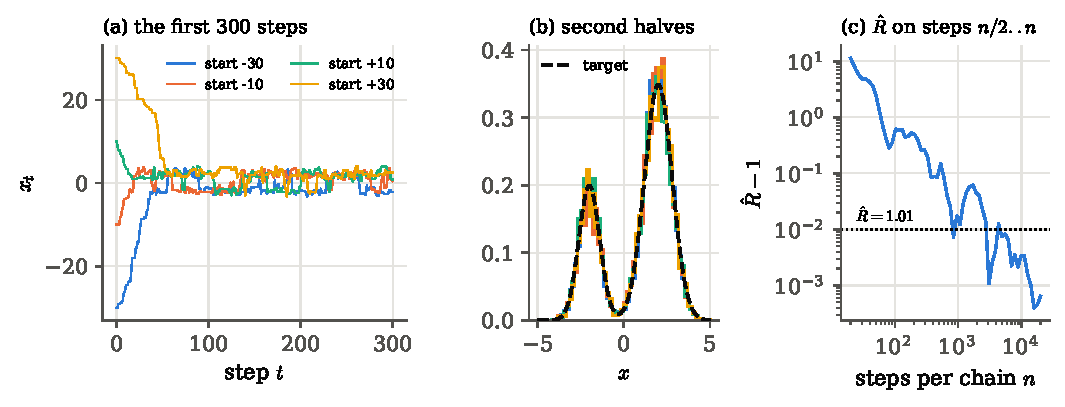
\includegraphics[width=\linewidth]{figures/ch09/multichain.pdf}
\caption{Four Metropolis chains on the two-bump density, started at $-30$, $-10$, $+10$ and $+30$.
(a) The first 300 steps: every chain falls into the bumps and starts hopping between them.
(b) Histograms of the second halves of the four chains, with the target (dashed). (c) $\hat R-1$
on the second half of the steps so far, falling through the $1.01$ line.}
\label{9b:fig:multichain}
\end{figure}

\paragraph{Example: what $\hat R$ sees, and what it cannot see.}
Now move the bumps to $x=\pm6$, keep their widths, and use short steps of 0.5. The valley between
the bumps is now so deep that a walker essentially never crosses it. Four walkers from $-30$,
$-10$, $+10$ and $+30$ settle into the bump on their own side and stay there
(\cref{9b:fig:rhat-traps}a). Each chain on its own looks excellent: its trace is stationary, and
its autocorrelation time is only about $\NineBMcFarSingleTau$ steps. Only the comparison
between chains reveals the problem: $\hat R=\NineBMcFarRhat$.

Then start all four walkers on the right, at $8$, $12$, $20$ and $30$
(\cref{9b:fig:rhat-traps}b). They all fall into the right bump and agree perfectly:
$\hat R=\NineBMcSameRhat$. Their common mean is $\NineBMcSameMean$, while the true mean of the
target is $0.3\times(-6)+0.7\times6=\NineBMcFarMeanExact$. Thirty per cent of the probability
is in a bump that none of the walkers has seen, and no statistic computed from them can know.

\begin{figure}[htbp]
\centering
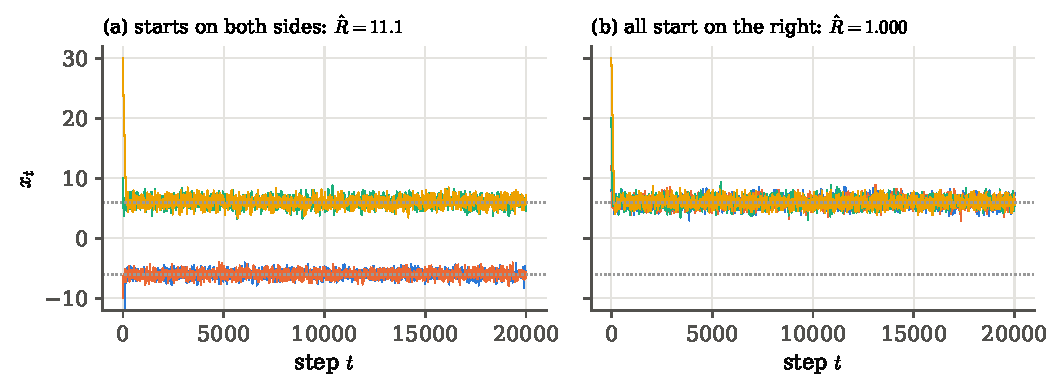
\includegraphics[width=\linewidth]{figures/ch09/rhat_traps.pdf}
\caption{The same test on a target with bumps at $\pm6$ (dotted), sampled with short steps.
(a) Chains started on both sides stay on their own side; $\hat R$ is far above one and exposes
the problem. (b) Chains all started on the right agree with each other perfectly and $\hat R$ is
one, yet all of them miss the left bump.}
\label{9b:fig:rhat-traps}
\end{figure}

\begin{pitfall}[$\hat R\simeq1$ is necessary, not sufficient]
$\hat R$ compares chains with each other. It detects chains that disagree; it cannot detect
chains that agree on the wrong answer because none of them reached part of the posterior
\srcref{Kruschke}{§7.5.1}. Start the chains genuinely overdispersed, wider than any plausible
posterior and on all sides of it, and be most suspicious when the posterior may have several
separated modes. The same trap reappears in physics as broken ergodicity: a double well at low
temperature (\cref{9b:sec:canonical}).
\end{pitfall}

Lambert distinguishes the two ways chains can fail to converge \srcref{Lambert}{§13.9.4}: poor
mixing \emph{between} chains, as in \cref{9b:fig:rhat-traps}a, which ordinary $\hat R$ catches;
and poor mixing \emph{within} a chain, a chain whose first half and second half disagree because
it is still drifting, which only split-$\hat R$ catches. \textcite{BrooksGelman1998} extended the
diagnostic to many parameters at once; modern practice computes split-$\hat R$ for every
parameter, together with the ESS of \cref{9b:sec:tau}.
\section{Forgetting the start is not forgetting the prior}
\label{9b:sec:start-prior}

Two things in an MCMC analysis are chosen before any step is taken, and both are sometimes loosely
called ``initial conditions'': the point where the walker starts, and the prior. It is easy to
think that a long enough chain forgets both. It forgets only one of them.

The starting point is forgotten by the chain. That is ergodicity (\cref{9a:sec:convergence}):
for an irreducible aperiodic chain the distribution of $X_t$ approaches the stationary
distribution geometrically fast from any start (the Doeblin contraction of
\cref{9a:sec:doeblin}), and the three crowds of the AR(1) chain, started twenty standard
deviations apart, ended with the same histogram (\cref{9a:sec:ar1-forgetting}). The four walkers
of \cref{9b:sec:rhat} did the same on the two bumps.

The prior is not part of the walk; it is part of the target. The walker samples
$f(\params)\propto\Like(\params)\,p(\params)$, and a different prior is a different $f$. A chain
run with a wrong prior converges, faithfully and from any start, to the posterior of that wrong
prior. Running it longer only makes the wrong answer more precise. What forgets the prior is more
\emph{data}: the likelihood is a product over data points and grows sharper as their number $N$
grows, while the prior stays as it is, so for large $N$ the posterior is governed by the
likelihood. That is the Bernstein--von Mises statement of \cref{ch:05}.

A physicist has met this distinction before. A gas in a box forgets its initial microstate as it
thermalises. It does not forget its Hamiltonian: an external potential added to the Hamiltonian
changes the equilibrium state, and waiting longer only brings the gas closer to the equilibrium
of that Hamiltonian. In the language of \cref{9b:sec:ratios}, $-\ln f=-\ln\Like-\ln p$ plays the
role of the energy, and the prior is a fixed external potential $-\ln p$ that the data's
potential $-\ln\Like$, growing in proportion to $N$, eventually overwhelms.

\begin{figure}[htbp]
\centering
\begin{tikzpicture}[node distance=6mm and 9mm,
  box/.style={draw=black!45,rounded corners=2pt,align=center,font=\small,inner sep=4pt,
              minimum height=10mm},
  arr/.style={->,thick,black!60}]
  \node[box] (start) {starting point $x_0$};
  \node[box,right=of start] (chain) {run the chain\\ longer};
  \node[box,right=of chain,fill=tangentgreen!10] (post) {the posterior\\ $\propto\Like\,p$};
  \draw[arr] (start) -- (chain);
  \draw[arr] (chain) -- (post);
  \node[box,below=12mm of start] (prior) {prior $p(\params)$};
  \node[box,right=of prior] (target) {part of the\\ target $f\propto\Like\,p$};
  \node[box,right=of target,fill=bdryred!8] (wrong) {posterior of\\ \emph{that} prior};
  \draw[arr] (prior) -- (target);
  \draw[arr] (target) -- (wrong);
  \node[box,below=12mm of target] (data) {more data:\\ $\ln\Like$ grows as $N$};
  \node[box,right=of data,fill=tangentgreen!10] (bvm) {prior's pull\\ shrinks as $1/\sqrt N$};
  \draw[arr] (data) -- (bvm);
  \draw[arr,dashed] (data.north) -- (target.south);
  \node[font=\footnotesize,anchor=west,text=softgray] at ($(post.east)+(1mm,0)$) {forgotten};
  \node[font=\footnotesize,anchor=west,text=softgray] at ($(wrong.east)+(1mm,0)$) {kept};
  \node[font=\footnotesize,anchor=west,text=softgray] at ($(bvm.east)+(1mm,0)$) {forgotten};
\end{tikzpicture}
\caption{Two different kinds of forgetting. Top: the starting point is erased by running the chain
(ergodicity). Middle: the prior is built into the target, so running the chain longer leads to the
posterior of that prior. Bottom: only more data, through a likelihood that sharpens with $N$,
reduce the prior's influence.}
\label{9b:fig:forget-schema}
\end{figure}

\paragraph{The question.} Can we see both statements in one experiment? Same data; two priors,
one sensible and one confidently wrong; several chains from wildly different starting points; few
data and many data.

\paragraph{The experiment.}
A detector counts events from a Poisson process with true rate $\lambda=\NineBSpTrue$ per unit
exposure; this is the counting situation of a collider bin or a photon detector (\cref{ch:02}).
We observe $N$ exposures with counts $n_1,\dots,n_N$ and total $S=\sum_in_i$. Two priors for
$\lambda$:
\begin{itemize}[itemsep=1pt]
  \item[A:] flat on $\lambda>0$;
  \item[B:] confident and wrong, $\ln\lambda\sim\Normal(\ln10,0.2^2)$, that is,
        ``$\lambda$ is $10$, give or take 20\%''.
\end{itemize}
The log posterior, up to a constant, is
\begin{equation}
  \ln f(\lambda)=\underbrace{S\ln\lambda-N\lambda}_{\ln\Like}+\ln p(\lambda),
  \qquad
  \ln p_B(\lambda)=-\ln\lambda-\frac{(\ln\lambda-\ln10)^2}{2\times0.2^2},
  \label{9b:eq:poisson-post}
\end{equation}
where the Poisson likelihood $\prod_ie^{-\lambda}\lambda^{n_i}/n_i!$ contributes $S\ln\lambda-N\lambda$
after dropping the $n_i!$, which do not depend on $\lambda$, and $\ln p_B$ includes the Jacobian
$1/\lambda$ of the log-normal density. Under prior A the posterior is known exactly:
\begin{align*}
  p_A(\lambda\given\data)
  &\eqby{1}\frac{\lambda^Se^{-N\lambda}}{\int_0^\infty t^Se^{-Nt}\dd t}
   \eqby{2}\frac{N^{S+1}}{S!}\,\lambda^Se^{-N\lambda},
  \qquad
  \E_A(\lambda\given\data)\eqby{3}\frac{S+1}{N}.
\end{align*}
\begin{explain}
  \item Likelihood times a flat prior, normalised.
  \item $\int_0^\infty t^Se^{-Nt}\dd t=S!/N^{S+1}$ (substitute $u=Nt$; Gamma integral).
  \item The mean of a Gamma density with shape $S+1$ and rate $N$; the same integral with $S+1$
        in place of $S$.
\end{explain}
Under prior B the posterior is computed by one-dimensional quadrature on a fine grid, as the
reference. For each prior and each data set we run four Metropolis--Hastings chains of
$\NineBSpN$ steps with multiplicative steps $\lambda\to\lambda e^{sZ}$ and the Hastings factor
$y/x$ of \cref{9b:sec:hastings}, started at $\lambda_0=0.05$, $1$, $40$ and $200$, four decades
apart.

\paragraph{Few data: the start is forgotten, the prior is not.}
With $N=3$ exposures the counts were $(\NineBSpCountsFew)$, $S=\NineBSpFewSum$; these happen to
be low for a true rate of 4, as three Poisson counts easily are. Within some tens of steps the
four chains from four decades apart have merged (\cref{9b:fig:start-prior}a), and their
second-phase means differ by only $\NineBSpFewBSpread$; $\hat R=\NineBSpFewBRhat$ for prior B
and $\NineBSpFewARhat$ for prior A. The starting points are gone. The priors are not. The
posterior mean is $\NineBSpFewAMean$ under A (exact $(S+1)/N=\NineBSpFewAMeanExact$) and
$\NineBSpFewBMean$ under B (quadrature: $\NineBSpFewBMeanExact$), $\NineBSpFewShift$ posterior
standard deviations apart (\cref{9b:fig:start-prior}c). Running prior B ten times longer,
$\NineBSpLongN$ steps, gives $\NineBSpLongMean$: no movement at all towards the truth, because
there is nothing for it to move towards. The chain has already found its target.

\paragraph{Many data: the likelihood takes over.}
With $N=300$ exposures, $S=\NineBSpManySum$. The chains again forget their starts, more slowly
now because the posterior is narrow and the steps small (\cref{9b:fig:start-prior}b). And now the
two priors nearly agree: $\NineBSpManyAMean$ under A (exact $\NineBSpManyAMeanExact$) and
$\NineBSpManyBMean$ under B, only $\NineBSpManyShift$ posterior standard deviations apart, both
close to the true 4 (\cref{9b:fig:start-prior}d). The data have outweighed even a prior that
claimed 10 within 20\%.

\begin{figure}[htbp]
\centering
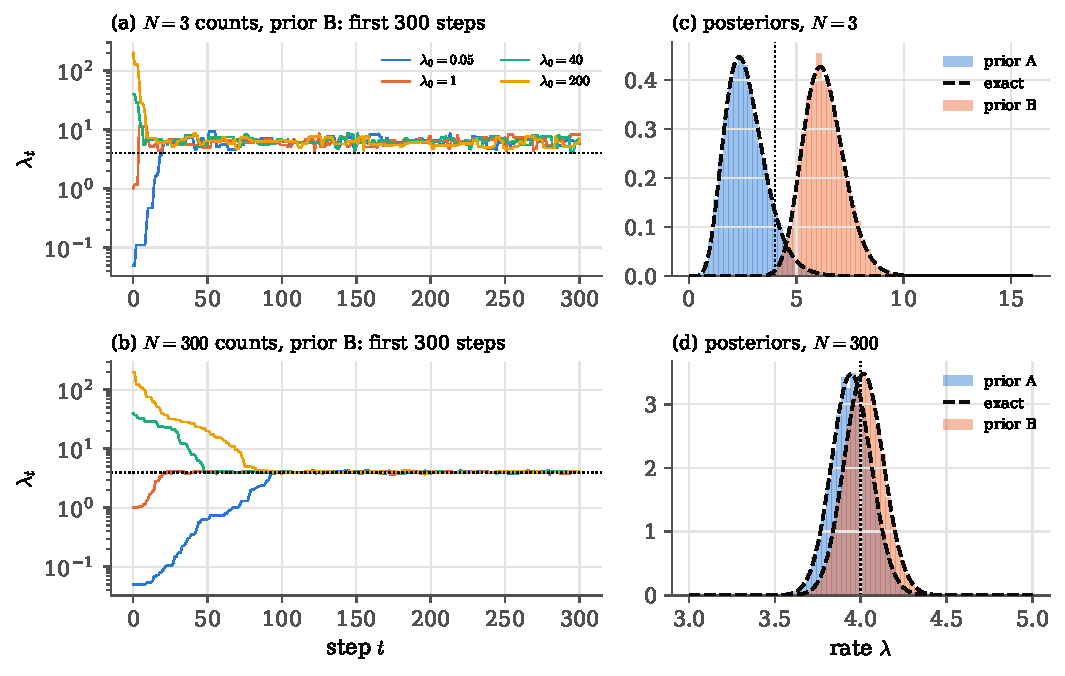
\includegraphics[width=\linewidth]{figures/ch09/start_vs_prior.pdf}
\caption{Starting point versus prior for a Poisson rate (true value 4, dotted). Left: the first
300 steps of four chains under the wrong prior B, started at $\lambda_0=0.05$, $1$, $40$ and $200$
(logarithmic axis); with 3 counts (a) and 300 counts (b) they merge, so the start is forgotten.
Right: posteriors from the chains (histograms) and exact (dashed) under the flat prior A and the
wrong prior B. With 3 counts (c) the two priors give different answers; with 300 counts (d) they
nearly agree.}
\label{9b:fig:start-prior}
\end{figure}

\paragraph{How fast is the prior forgotten?}
The rate can be predicted by expanding the log posterior around the peak of the likelihood. The
log likelihood $S\ln\lambda-N\lambda$ peaks at $\hat\lambda=S/N$ with curvature
$-S/\hat\lambda^2=-N/\hat\lambda$, so near the peak it is a Gaussian of variance
$\sigma_L^2=\hat\lambda/N$. Add the log prior, approximated by its tangent line at $\hat\lambda$:
\begin{align}
  \ln f(\lambda)
  &\eqby{1}\text{const}-\frac{(\lambda-\hat\lambda)^2}{2\sigma_L^2}
     +(\ln p)'(\hat\lambda)\,(\lambda-\hat\lambda)
  \nonumber\\
  &\eqby{2}\text{const}'-\frac{\bigl[\lambda-\hat\lambda-\sigma_L^2(\ln p)'(\hat\lambda)\bigr]^2}
     {2\sigma_L^2},
  \nonumber\\
  \frac{\text{shift}}{\text{width}}
  &\eqby{3}\frac{\sigma_L^2\,(\ln p)'(\hat\lambda)}{\sigma_L}
   =\sqrt{\frac{\hat\lambda}{N}}\;(\ln p)'(\hat\lambda).
  \label{9b:eq:prior-shift}
\end{align}
\begin{explain}
  \item Second-order Taylor expansion of $\ln\Like$ at its maximum, first-order expansion of
        $\ln p$, valid when the posterior is narrow compared with the scale on which the prior
        changes.
  \item Complete the square; the constant absorbs everything independent of $\lambda$.
  \item The posterior peak moves by $\sigma_L^2(\ln p)'$ while its width stays $\sigma_L$.
\end{explain}
The prior's pull, measured in posterior widths, shrinks as $1/\sqrt N$.

\emph{The slope of the wrong prior.} To use \eqref{9b:eq:prior-shift} for prior B we need the
derivative of its log density, $\ln p_B(\lambda)=-\ln\lambda-(\ln\lambda-\ln10)^2/(2\times0.2^2)$,
at the true rate $\lambda\simeq4$:
\begin{align*}
  (\ln p_B)'(\lambda)
  &\eqby{1}-\frac1\lambda-\frac{2(\ln\lambda-\ln10)}{2\times0.2^2}\cdot\frac1\lambda
   \eqby{2}-\frac1\lambda-\frac{\ln\lambda-\ln10}{0.04\,\lambda},
  \\
  (\ln p_B)'(4)
  &\eqby{3}-0.25-\frac{-0.916}{0.04\times4}
   =-0.25+5.73\simeq5.5 .
\end{align*}
\begin{explain}
  \item The first term is the Jacobian $1/\lambda$ of the log-normal density, whose log has
        derivative $-1/\lambda$. The second is a square: chain rule, with
        $\dd(\ln\lambda)/\dd\lambda=1/\lambda$.
  \item $2\times0.2^2/2=0.2^2=0.04$, the prior's variance in $\ln\lambda$.
  \item $\ln4-\ln10=\ln0.4=-0.916$.
\end{explain}
The Jacobian term is small; the second term dominates because $\lambda=4$ lies $0.916/0.2\simeq4.6$
prior standard deviations below the prior's centre at 10. The slope is positive: the prior
pulls the posterior peak upwards, towards 10. With
$N=300$, $\hat\lambda\simeq3.94$, \eqref{9b:eq:prior-shift} predicts a shift of
$\sqrt{3.94/300}\times5.5\simeq0.63$ widths, matching the $\NineBSpManyShift$ found by the chains.
For $N=3$ the expansion is not valid (the posterior is as wide as the prior), and the chains are
the only honest answer. The result is the one-parameter form of the Bernstein--von Mises theorem
of \cref{ch:05}.

\begin{keyidea}[Two kinds of forgetting]
A Markov chain forgets its starting point because it is ergodic, and running it longer completes
the forgetting. It does not forget the prior, because the prior is part of the distribution it
samples; running longer only converges more precisely to the posterior of that prior. The prior's
influence fades only as the data accumulate, as $1/\sqrt N$ in units of the posterior width.
\end{keyidea}

Two practical consequences follow. First, a convergence diagnostic such as $\hat R$ tests the
chain, never the prior: in the experiment above $\hat R$ was $\NineBSpFewBRhat$ for the wrong
prior with three counts. Checking a prior is a modelling question, answered by trying
alternatives and seeing how much the posterior moves (a prior sensitivity analysis), or by
importance-reweighting the existing chain to the new prior (\cref{ch:06}) when the two posteriors
overlap. Second, the experiment explains why cosmological analyses report which priors they used
on poorly constrained parameters, such as the optical depth to reionisation in a CMB analysis
without large-scale polarisation: there the data are ``few'' for that parameter, and the prior
still shows in the answer.

\begin{pitfall}[``Burn-in will take care of the prior'']
Burn-in removes the memory of the starting point, nothing else. If two analyses of the same data
with different priors disagree, no amount of running will reconcile them; only more informative
data will, and only to the extent \eqref{9b:eq:prior-shift} allows.
\end{pitfall}
\section{Back to statistical mechanics: sampling the canonical ensemble}
\label{9b:sec:canonical}

Recall the oscillator of fixed energy (\cref{9a:sec:oscillator}): a mass on a
spring, $x(t)=A\cos(\omega t+\varphi)$, looked at at random instants. Its own motion did the
sampling. Every point of the energy ellipse in phase space is visited once per period, the time
spent near $x$ is proportional to $1/\abs v$, and the histogram of $x$ is the arcsine law
$1/(\pi\sqrt{A^2-x^2})$ of \eqref{9a:eq:arcsine}. That is the \newterm{microcanonical} ensemble:
the energy is fixed, and the states on the energy shell are weighted by the time the motion
spends in them.

Now put the same oscillator in contact with a heat bath at temperature $T$, a large reservoir it
can exchange energy with. Its energy is no longer fixed. Statistical mechanics says that the
probability density of a phase-space point $(x,p)$ is then the \newterm{canonical}, or Boltzmann,
density
\begin{equation}
  \rho(x,p)=\frac{e^{-H(x,p)/kT}}{Z},\qquad Z=\int e^{-H(x,p)/kT}\,\dd x\,\dd p ,
  \label{9b:eq:canonical}
\end{equation}
with $H$ the Hamiltonian, $k$ Boltzmann's constant and $Z$ the partition function. In this
section $\rho$ is this Boltzmann density (not an autocorrelation) and $p$ is the momentum (not a
prior or posterior). The
oscillator's own Hamiltonian motion cannot produce this density. Hamilton's equations conserve
$H$, so a trajectory started on one energy shell stays on it forever and never visits the others.
In nature the energy changes through collisions with the bath. On a computer something else must
change it, and that something is the Metropolis walker. This is the problem for which
\textcite{Metropolis1953} invented the algorithm: to compute canonical averages, an equation of
state, for a system of interacting particles, where neither the partition function nor a direct
way to draw configurations is available.

\begin{center}
\small
\begin{tabular}{@{}p{0.25\linewidth}p{0.33\linewidth}p{0.33\linewidth}@{}}
\toprule
 & microcanonical & canonical \\
\midrule
what is fixed & energy $E$ & temperature $T$ (energy exchanged with a bath) \\
distribution & uniform on the shell $H=E$, weighted by time & $e^{-H/kT}/Z$ over all of phase space \\
who samples it & the system's own dynamics (if ergodic) & a Metropolis walker; physically, the bath \\
oscillator's $x$ & arcsine law on $\abs x<A$ & Gaussian, variance $kT/m\omega^2$ \\
\bottomrule
\end{tabular}
\end{center}

\paragraph{The question.} Run Metropolis on $e^{-H/kT}$. Does it reproduce what statistical
mechanics predicts where we can calculate (the oscillator), and how does it behave where we cannot
(a double well, and a lattice of interacting spins)?

The decision ratio of the walker is
\begin{equation}
  R=\frac{\rho(y)}{\rho(x)}=\frac{e^{-H(y)/kT}/Z}{e^{-H(x)/kT}/Z}=e^{-[H(y)-H(x)]/kT}:
  \label{9b:eq:boltzmann-ratio}
\end{equation}
a move that lowers the energy is always taken, and a move that raises it by $\Delta H$ is taken
with probability $e^{-\Delta H/kT}$. The partition function cancels exactly as the evidence did in
\eqref{9b:eq:ratio}. The two problems are the same problem in two vocabularies:
\begin{center}
\small
\begin{tabular}{@{}ll@{}}
\toprule
Bayesian inference & statistical mechanics \\
\midrule
posterior $p(\params\given\data)$ & Boltzmann density $\rho$ \\
$-\ln\bigl[\Like(\params)\,p(\params)\bigr]$ & energy in units of $kT$, $H/kT$ \\
evidence $Z=\int\Like\,p\,\dd\params$ & partition function $Z=\int e^{-H/kT}$ \\
tempered target $f^\beta$ (\cref{9b:sec:balance}) & Boltzmann weight at temperature $1/\beta$ \\
maximum a posteriori point & ground state \\
posterior mean of $g$ & thermal average $\langle g\rangle$ \\
\bottomrule
\end{tabular}
\end{center}

\subsection{The harmonic oscillator in a heat bath}
\label{9b:sec:canon-osc}

For $H=p^2/2m+m\omega^2x^2/2$ the canonical density factorises into two Gaussians, so every
prediction can be written down. (We write the spring as $m\omega^2$ to keep the letter $k$ for
Boltzmann's constant.)
\begin{align}
  \rho(x,p)
  &\eqby{1}\frac1Z\exp\Bigl(-\frac{p^2}{2mkT}\Bigr)\exp\Bigl(-\frac{x^2}{2kT/m\omega^2}\Bigr),
  \nonumber\\
  \Bigl\langle\frac{p^2}{2m}\Bigr\rangle
  &\eqby{2}\frac{mkT}{2m}=\frac{kT}2,
  \qquad
  \Bigl\langle\frac{m\omega^2x^2}{2}\Bigr\rangle
   \eqby{3}\frac{m\omega^2}{2}\,\frac{kT}{m\omega^2}=\frac{kT}2,
  \qquad
  \langle H\rangle=kT .
  \label{9b:eq:equipartition}
\end{align}
\begin{explain}
  \item $e^{-H/kT}=e^{-p^2/2mkT}\,e^{-m\omega^2x^2/2kT}$: $p$ and $x$ are independent Gaussians
        with variances $mkT$ and $kT/m\omega^2$.
  \item $\langle p^2\rangle$ is the variance of $p$, since its mean is zero.
  \item Likewise for $x$. Each quadratic term in $H$ carries $kT/2$: equipartition.
\end{explain}
The distribution of the energy itself follows from the area of phase space at each energy. The
region $H\le E$ is an ellipse with semi-axes $\sqrt{2E/m\omega^2}$ in $x$ and $\sqrt{2mE}$ in $p$,
so its area is $\mathcal A(E)=\pi\sqrt{2E/m\omega^2}\sqrt{2mE}=2\pi E/\omega$, and the area
between $E$ and $E+\dd E$ is $\mathcal A'(E)\,\dd E=(2\pi/\omega)\,\dd E$, the same for every
$E$: the one-dimensional oscillator has a constant density of states. Hence
\begin{equation}
  p(E)\propto e^{-E/kT}\,\frac{2\pi}{\omega}
  \quad\Longrightarrow\quad
  p(E)=\frac{1}{kT}\,e^{-E/kT},\qquad \Prob(E>2kT)=e^{-2}=0.135 .
  \label{9b:eq:energy-dist}
\end{equation}

\paragraph{Canonical from microcanonical.}
The two ensembles are not unrelated: the canonical one is a mixture of microcanonical shells,
each weighted by its Boltzmann probability \eqref{9b:eq:energy-dist}. On the shell of energy $E$
the position follows the arcsine law with amplitude $A=\sqrt{2E/m\omega^2}$. Averaging it over
$E$ should give back the Gaussian of \eqref{9b:eq:equipartition}. In units with $m\omega^2=1$
(so $A^2=2E$):
\begin{align}
  p(x)
  &\eqby{1}\int_{x^2/2}^\infty\frac{e^{-E/kT}}{kT}\;\frac{1}{\pi\sqrt{2E-x^2}}\,\dd E
   \eqby{2}\frac{e^{-x^2/2kT}}{2\pi kT}\int_0^\infty e^{-u/2kT}\,u^{-1/2}\,\dd u
  \nonumber\\
  &\eqby{3}\frac{e^{-x^2/2kT}}{2\pi kT}\,\Gamma\bigl(\tfrac12\bigr)\sqrt{2kT}
   \eqby{4}\frac{e^{-x^2/2kT}}{\sqrt{2\pi kT}} .
  \label{9b:eq:shell-mixture}
\end{align}
\begin{explain}
  \item Law of total probability over the energy: $p(x)=\int p(E)\,p(x\given E)\,\dd E$; only
        shells with $A>\abs x$, that is $E>x^2/2$, reach $x$.
  \item Substitute $u=2E-x^2$, so $E=(u+x^2)/2$ and $\dd E=\dd u/2$; the factor
        $e^{-x^2/2kT}$ comes out of the integral.
  \item $\int_0^\infty e^{-u/c}u^{-1/2}\dd u=\Gamma(\tfrac12)\sqrt c$ with $c=2kT$.
  \item $\Gamma(\tfrac12)=\sqrt\pi$, and $\sqrt\pi\sqrt{2kT}/(2\pi kT)=1/\sqrt{2\pi kT}$.
\end{explain}
The arcsine laws, each piled up at its own turning points, add up to a Gaussian peaked at the
centre. The same Hamiltonian gives two different distributions of $x$ because the sampling
prescription is different: a random instant at fixed energy, or a random state at fixed
temperature.

\paragraph{The walker in phase space.}
A Metropolis walker in the plane $(x,p)$, with $m=\omega=1$, $kT=1$, round steps of width
$2.38/\sqrt2$, started at $(3,-3)$ and run for $\NineBCaN$ steps, accepted $\NineBCaAcc$ of its
proposals (\cref{9b:fig:canon-osc}). It never uses $Z$ and knows nothing about shells or
equipartition. It gives $\Var x=\NineBCaVarX$ and $\Var p=\NineBCaVarP$ (exact: $kT=1$), kinetic
and potential energies $\langle p^2/2\rangle=\NineBCaKin$ and $\langle x^2/2\rangle=\NineBCaPot$
(exact: $1/2$ each), $\langle H\rangle=\NineBCaE$, a fraction $\NineBCaFracHot$ of states with
$E>2kT$ (exact $e^{-2}=\NineBCaFracHotExact$), and a correlation of $\NineBCaCorrXP$ between $x$
and $p$ (exact 0). Drawing instead an energy from $p(E)$ and a uniform phase on that shell, as in
\eqref{9b:eq:shell-mixture}, gives $\Var x=\NineBCaShellVar$: the mixture of microcanonical
ensembles is the canonical one.

\begin{figure}[htbp]
\centering
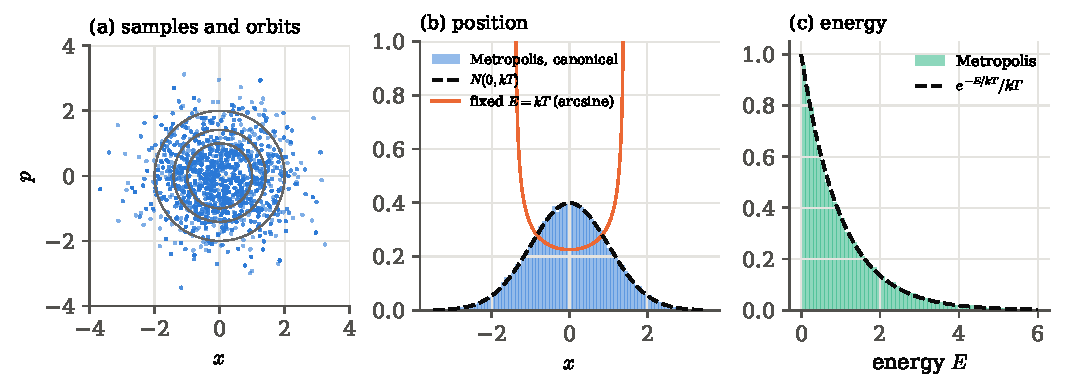
\includegraphics[width=\linewidth]{figures/ch09/canonical_oscillator.pdf}
\caption{Metropolis for the oscillator at $kT=1$. (a) The first 3000 states in phase space, with
three energy shells: the walker crosses shells freely, which the Hamiltonian motion never does.
(b) Position: the canonical histogram is the Gaussian $\Normal(0,kT)$ (dashed), not the arcsine
law of a single shell at $E=kT$ (orange). (c) Energy: exponential, $e^{-E/kT}/kT$.}
\label{9b:fig:canon-osc}
\end{figure}

\begin{keyidea}[Dynamics samples the shell, Metropolis samples the ensemble]
Hamiltonian motion conserves energy, so at best it samples one microcanonical shell, uniformly in
time. The canonical density $e^{-H/kT}/Z$ is a mixture of all shells weighted by $e^{-E/kT}$ times
the density of states. A Metropolis walker samples it directly, because its acceptance rule
$\min(1,e^{-\Delta H/kT})$ plays the part of the heat bath: it lets the energy change, and makes
rises in energy exponentially rare. The partition function, like the evidence, never appears.
\end{keyidea}

\subsection{A double well: no formula, and a barrier}
\label{9b:sec:double-well}

Replace the spring by the potential $V(x)=\Delta V\,(x^2-1)^2$, with minima at $x=\pm1$ and a
barrier of height $\Delta V=\NineBDwBarrier$ at $x=0$: a particle in a symmetric double well, the
shape of a molecule with two conformations or of an order parameter below a phase transition. The
momentum part of $e^{-H/kT}$ is the same Gaussian as before and factorises away, so the question
is the position density $\rho(x)\propto e^{-V(x)/kT}$. Its normalisation $\int e^{-V/kT}\dd x$
has no elementary closed form. In one dimension we can still compute it by quadrature as a check;
in a thousand dimensions we could not, but the walker would not notice the difference.

With $\NineBDwN$ steps of width $0.15$ the walker reproduces $e^{-V/kT}$ at all temperatures
(\cref{9b:fig:double-well}a): $\langle x^2\rangle=\NineBDwHotXsqMC$ at $kT=1$ (quadrature
$\NineBDwHotXsqExact$) and $\NineBDwColdXsqMC$ at $kT=0.25$ ($\NineBDwColdXsqExact$), with
fractions $\NineBDwHotRight$ and $\NineBDwColdRight$ of the time in the right well (exact
$\tfrac12$ by symmetry). But the way it gets there changes with temperature. At $kT=0.25$ the
barrier is four times $kT$, and the walker spends long stretches in one well before hopping to
the other (\cref{9b:fig:double-well}b): $\NineBDwColdHops$ hops per $10^5$ steps, against
$\NineBDwHotHops$ at $kT=1$.

\paragraph{How rare are the hops?}
A walker that moves in small steps behaves like a diffusing particle, and the rate at which it
crosses the barrier follows the same reasoning as a thermally activated chemical reaction. To
hop, the walker must first be near the top of the barrier, and must then diffuse across it. We
estimate the two pieces separately and multiply.

\emph{How often is the walker at the top?} Call the strip of width $w$ around the top of the
barrier, centred on $x=0$, the top region. In equilibrium the probability of being in it is the
Boltzmann weight integrated over the strip, divided by the integral over everything. The
denominator is dominated by the two wells. Near a minimum, $V(x)\simeq V''(1)(x-1)^2/2$ (the
minimum value is 0), so each well contributes a Gaussian integral:
\begin{align*}
  \Prob(\text{top})
  &\eqby{1}\frac{\int_{\rm strip}e^{-V(x)/kT}\,\dd x}{\int e^{-V(x)/kT}\,\dd x}
   \eqby{2}\frac{e^{-\Delta V/kT}\,w}{2Z_{\rm well}},
  \qquad
  Z_{\rm well}\eqby{3}\int e^{-V''(1)(x-1)^2/2kT}\,\dd x=\sqrt{\frac{2\pi kT}{V''(1)}} .
\end{align*}
\begin{explain}
  \item The fraction of time in a region is the integral of the normalised density $\rho(x)$
        over it.
  \item Inside the strip $V$ is within about $kT$ of its maximum $\Delta V$, so
        $e^{-V/kT}\simeq e^{-\Delta V/kT}$ up to a factor of order one, and the integral is that
        value times the width. The two wells each contribute $Z_{\rm well}$.
  \item The Gaussian integral $\int e^{-u^2/2\sigma^2}\dd u=\sqrt{2\pi}\,\sigma$ with
        $\sigma^2=kT/V''(1)$.
\end{explain}

\emph{How wide is the top?} Near $x=0$ the potential is a downward parabola,
$V(x)\simeq\Delta V-\abs{V''(0)}\,x^2/2$. The top region is where the walker is within $kT$ of the
summit, where nothing pushes it strongly either way:
\begin{equation*}
  \frac{\abs{V''(0)}\,x^2}{2}\le kT
  \quad\iff\quad
  \abs x\le\sqrt{\frac{2kT}{\abs{V''(0)}}},
  \qquad
  w=2\sqrt{\frac{2kT}{\abs{V''(0)}}} .
\end{equation*}
A hotter walker has a wider top, $w\propto\sqrt{kT}$.

\emph{How long does it take to cross?} A Metropolis walker with steps $s$ much smaller than the
scale of $V$ accepts nearly every step, and so moves like the drunkard of \cref{9a:sec:diffusion}:
its mean squared displacement after $t$ steps is $s^2t$. Writing that as $2Dt$ defines its
diffusion constant $D=s^2/2$ per step (here $D$ is a diffusion constant, not a dimension).
Crossing a strip of width $w$ by diffusion takes about $t_{\rm cross}=w^2/2D$ steps, the
diffusive cost $(L/s)^2$ again.

\emph{Multiply.} The hop rate per step is the probability of being at the top divided by the time
it takes to cross it:
\begin{align}
  \text{rate}
  &\eqby{1}\frac{\Prob(\text{top})}{t_{\rm cross}}
   =\frac{e^{-\Delta V/kT}\,w}{2Z_{\rm well}}\cdot\frac{2D}{w^2}
   =\frac{D\,e^{-\Delta V/kT}}{w\,Z_{\rm well}}
  \nonumber\\
  &\eqby{2}\frac{D\,e^{-\Delta V/kT}}{2\sqrt{2kT/\abs{V''(0)}}\;\sqrt{2\pi kT/V''(1)}}
   \eqby{3}\frac{\sqrt{\abs{V''(0)}\,V''(1)}}{4\sqrt\pi}\;\frac{D}{kT}\;e^{-\Delta V/kT}.
  \label{9b:eq:kramers}
\end{align}
\begin{explain}
  \item A walker in the strip leaves it, to one side or the other, after about $t_{\rm cross}$
        steps, so the strip is crossed about $\Prob(\text{top})/t_{\rm cross}$ times per step.
  \item Insert $w$ and $Z_{\rm well}$.
  \item $\sqrt{kT}\times\sqrt{kT}=kT$: the two square roots, one from the width of the top and
        one from the width of a well, combine into a single $1/kT$; everything else is a
        constant of the potential and of the step size.
\end{explain}
The prefactor $1/(4\sqrt\pi)\simeq0.14$ comes from our rough choice of the strip; a careful
treatment of the same problem replaces it by $1/(2\pi)\simeq0.16$, and leaves the dependence on
temperature unchanged. The result is the form of Kramers' rate for an overdamped particle
\parencite{Kramers1940}. Taking logarithms, $\ln(\text{rate}\times kT)=\text{const}-\Delta V/kT$,
so plotted against $\Delta V/kT$ it is a straight line of slope $-1$: every additional $kT$ of
barrier height makes hops $e\simeq2.7$ times rarer. The walker gives
slope $\NineBDwSlope$ for $kT\le0.5$ (\cref{9b:fig:double-well}c): Arrhenius's law, recovered from
a sampling algorithm.

\begin{figure}[htbp]
\centering
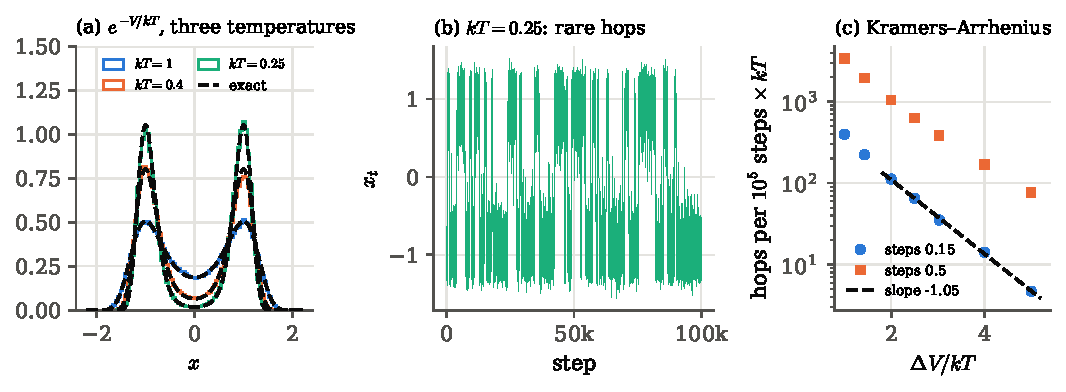
\includegraphics[width=\linewidth]{figures/ch09/double_well.pdf}
\caption{Metropolis on the double well $V=(x^2-1)^2$. (a) Histograms at three temperatures
against $e^{-V/kT}$ normalised by quadrature (dashed). (b) At $kT=0.25$ the walker stays in one
well for long stretches. (c) Hop rate times $kT$ against $\Delta V/kT$: small steps (dots) follow
the Kramers--Arrhenius line of slope $-1$ (dashed); large steps (squares) hop far more
often.}
\label{9b:fig:double-well}
\end{figure}

The squares in \cref{9b:fig:double-well}c are walkers with steps of $0.5$ instead of $0.15$.
They sample the same $e^{-V/kT}$ but hop far more often: $\NineBDwHopsColdBig$ hops per $10^5$
steps at $kT=0.25$, with a fitted slope of only $\NineBDwSlopeBig$. A step of that size can jump
from $x\simeq-0.6$ straight to $x\simeq+0.6$, where $V=\NineBDwVBig$, without ever visiting the
top of the barrier. A Metropolis walker is not a physical particle, and its steps are not physical
time. That is a strength for sampling, since moves that no real particle could make may cross
barriers cheaply (parallel tempering and cluster moves exploit this), and a warning for dynamics:
rates and time correlations read off an MCMC run are properties of the algorithm, not of the
system.

\begin{pitfall}[MCMC time is not physical time]
The stationary distribution of a Metropolis chain is the Boltzmann (or posterior) density; its
\emph{path} is not a trajectory of the physical system. Equilibrium averages from the chain are
physical; hop rates, relaxation times and autocorrelations depend on the proposal and are
diagnostics of the sampler. At low temperature the slow hops are also a sampling hazard: a chain
that has not hopped often enough is the broken-ergodicity trap of \cref{9b:fig:rhat-traps}.
\end{pitfall}

\subsection{The Ising model: a distribution nobody can sample directly}
\label{9b:sec:ising}

An $L\times L$ square lattice carries a spin $s_i=\pm1$ at each site, with periodic boundaries.
Neighbouring spins prefer to align; the energy of a configuration $s=(s_1,\dots,s_{L^2})$ is
\begin{equation}
  E(s)=-J\sum_{\langle ij\rangle}s_is_j ,
  \label{9b:eq:ising}
\end{equation}
where $\langle ij\rangle$ runs over nearest-neighbour pairs and $J>0$. For $L=\NineBIsL$ there
are $2^{\NineBIsSites}\simeq10^{\NineBIsLogConfigs}$ configurations. The partition function is a
sum over all of them, and no method of drawing configurations directly from $e^{-E/kT}/Z$ is
known for general temperatures. A grid in configuration space is not even conceivable.

\emph{The exact answer we compare with.} Yet the model has been solved exactly, in a limit: an
infinite lattice in zero external field. \textcite{Onsager1944} computed its partition function
per spin, by writing the sum over configurations row by row as a product of transfer matrices
and finding their largest eigenvalue; from the free energy follows the energy per spin
$u=\langle E\rangle/L^2$, measured in units of $J$. \textcite{Yang1952} computed the spontaneous
magnetisation, the mean spin $M=\langle s_i\rangle$ that the lattice keeps on its own when no
field is applied. Both calculations run to many pages and we do not repeat them: we use their
results as targets. They say that below the critical temperature
\begin{equation}
  kT_c=\frac{2J}{\ln(1+\sqrt2)}=\NineBIsTc\,J
  \label{9b:eq:tc}
\end{equation}
the spins order, with magnetisation per spin $M(T)=\bigl[1-\sinh^{-4}(2J/kT)\bigr]^{1/8}$, and
above it $M=0$. This is a perfect test: a distribution with no direct sampler and an exact answer.

\paragraph{The single-spin-flip walker.}
The walker proposes to flip one spin, $s_i\to-s_i$; the proposal is symmetric (flipping it back
is equally likely). Only the four bonds that touch site $i$ change. Before the flip they
contribute $-Js_ih_i$, with $h_i=\sum_{j\text{ nb } i}s_j$ the sum of the four neighbours; after
it, $+Js_ih_i$. So
\begin{equation}
  \Delta E=2Js_ih_i\in\{-8J,-4J,0,4J,8J\},
  \qquad
  a=\min\bigl(1,e^{-\Delta E/kT}\bigr),
  \label{9b:eq:ising-flip}
\end{equation}
a local computation that never needs $Z$. The code visits the sites in order:

\pyfile[firstline=20,lastline=35]{code/ch09/20_ising.py}{One Metropolis sweep of the Ising
lattice}

A systematic sweep is not one reversible chain, but it does not need to be. Each single-site
update satisfies detailed balance with $e^{-E/kT}$ and therefore leaves it stationary, and a
sequence of updates that each leave a distribution unchanged leaves it unchanged as a whole:
if $\pi P_1=\pi$ and $\pi P_2=\pi$, then $\pi P_1P_2=\pi P_2=\pi$.

\paragraph{The run.}
On a finite lattice the sign of the magnetisation flips now and then, so we record the mean of
its absolute value, $\langle\abs m\rangle$ with $m=\frac1{L^2}\sum_is_i$, and the mean energy per
spin. The settings are
\begin{center}
\begin{tabular}{lp{0.62\linewidth}}
\toprule
lattice & $L=\NineBIsL$, $\NineBIsSites$ spins, periodic boundaries\\
start & all spins up, at the lowest temperature\\
temperatures & twelve, from $kT=1.5J$ to $3.5J$, denser near $T_c$; each starts from the
last configuration of the one before (heating)\\
burn-in & $\NineBIsBurn$ sweeps at each temperature\\
measurement & $\NineBIsMeas$ sweeps at each temperature\\
\bottomrule
\end{tabular}
\end{center}
A sweep is one pass of the code above, one proposed flip per site.

\paragraph{Side by side.}
\Cref{9b:fig:ising} shows the whole scan; at one temperature on each side of $T_c$ the numbers are
\begin{center}
\begin{tabular}{lcccc}
\toprule
 & \multicolumn{2}{c}{$kT=1.8J$ (ordered)} & \multicolumn{2}{c}{$kT=3J$ (disordered)}\\
 & exact & ours & exact & ours\\
\midrule
$\langle\abs m\rangle$ & $\NineBIsMLowExact$ & $\NineBIsMLow$ & $0$ & $\NineBIsMHigh$\\
$u/J$ & $\NineBIsULowExact$ & $\NineBIsULow$ & $\NineBIsUHighExact$ & $\NineBIsUHigh$\\
accepted flips & & $\NineBIsAccLow$ & & $\NineBIsAccHigh$\\
\bottomrule
\end{tabular}
\end{center}
The snapshots show what the numbers mean: an ordered sea with a few flipped spins at $1.8J$,
domains of every size at $2.3J\approx T_c$, and short-range disorder at $3J$. At $1.8J$ almost
every proposed flip breaks four aligned bonds, $\Delta E=8J$ in \eqref{9b:eq:ising-flip}, and is
refused.

\paragraph{Why they differ.}
\emph{Statistical noise.} At $1.8J$ the magnetisations differ by $3\times10^{-4}$, and at $3J$ the
energies by $1.5\times10^{-3}$. The energy per spin of a lattice of a thousand spins fluctuates
by a few hundredths from sweep to sweep, and $\NineBIsMeas$ correlated sweeps average that down
to about $10^{-3}$: both differences are of the size of the run's own noise.

\emph{A magnetisation above $T_c$.} The exact $M=0$ is for an infinite lattice. A finite one has
a net magnetisation $m$ that fluctuates about zero, and the mean of its absolute value is
positive. If the $L^2$ spins were independent, $m$ would have standard deviation $1/L$ and
$\langle\abs m\rangle=\sqrt{2/\pi}/L\simeq0.025$ for $L=32$. At $3J$ each spin is correlated
with its neighbours over a few lattice spacings, which enlarges the fluctuation to the measured
$\NineBIsMHigh$. Either way it falls like $1/L$: a lattice twice as wide would give about half.

\emph{Rounding near $T_c$.} At $T_c$ the infinite lattice has domains of every size; ours cannot
hold a domain wider than $L=32$. The sharp corner of $M(T)$ is therefore smeared over a range of
temperatures in which the correlation length of the infinite lattice exceeds $L$, a few per cent
of $T_c$ for $L=32$, visible in \cref{9b:fig:ising}a as the dots leaving the exact curve before
$T_c$ and not reaching zero after it.

\emph{The ordered start.} A random start at low temperature would not reproduce Yang's curve.
The lattice orders locally into domains of both signs, and a band of down spins that wraps around
the periodic lattice can only be removed by moving its walls one spin at a time, which at
$1.8J$ may not happen within the run; $\langle\abs m\rangle$ would then come out far below
$0.96$. Starting ordered and heating keeps the lattice in the equilibrium state at every step of
the scan.

\emph{The lesson.} A walker that knows only the energy change of a single flip reproduces
Onsager's and Yang's infinite-lattice answers to the noise of the run, as long as the
temperature is not so close to $T_c$ that the lattice size itself matters.

\begin{figure}[htbp]
\centering
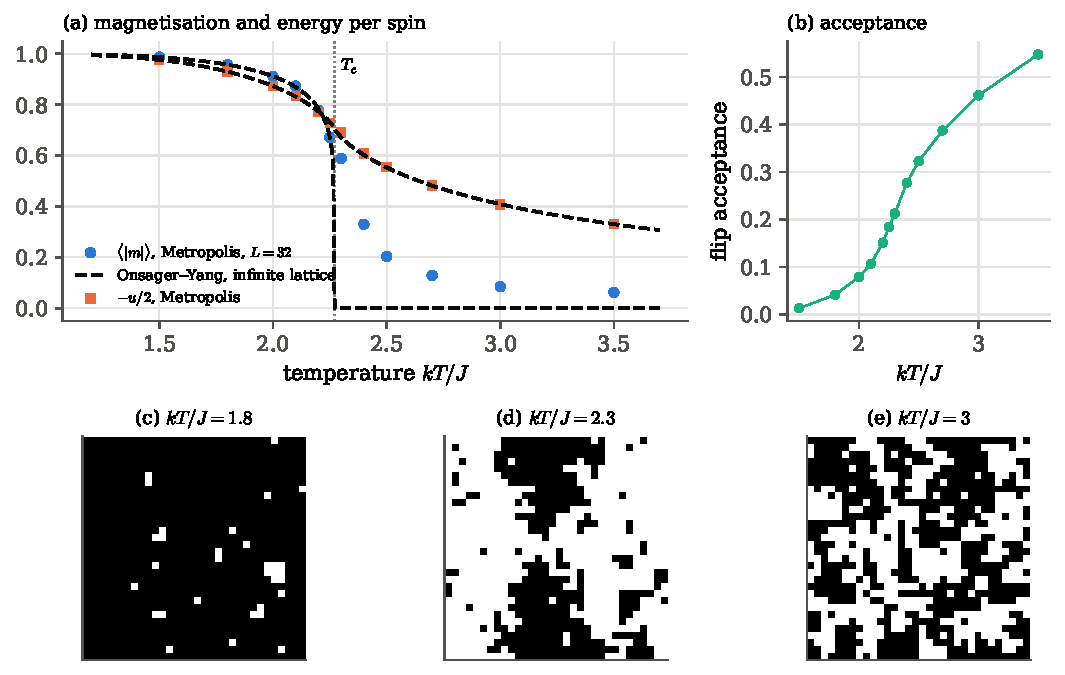
\includegraphics[width=\linewidth]{figures/ch09/ising.pdf}
\caption{The two-dimensional Ising model on a $32\times32$ lattice by single-spin-flip Metropolis.
(a) Mean absolute magnetisation per spin (dots) and minus half the energy per spin (squares)
against temperature, with the exact infinite-lattice results of Onsager and Yang (dashed); the
dotted line is $T_c$. (b) Fraction of accepted flips. (c)--(e) Configurations at three
temperatures (black and white are the two spin values).}
\label{9b:fig:ising}
\end{figure}

The whole scan takes seconds on a laptop: about $10^8$ spin updates, compiled with
\pyname{numba}. Research studies of the same model use lattices of $10^3$--$10^4$ sites per
side, many more sweeps near $T_c$, where the single-flip walker becomes very slow because
domains of all sizes must be rearranged one spin at a time, and cluster algorithms that flip
whole domains at once; they extract critical exponents from how the results change with $L$.
Underneath, the method is the same: a biased random walk through a space far too large to
enumerate, guided only by energy differences.
\section{Relatives of the biased walker: Gibbs, Hamiltonian and ensemble samplers}
\label{9b:sec:relatives}

Every walker so far proposed a random step and corrected it with the Metropolis--Hastings
decision. Its weakness was visible on the correlated ellipse of \cref{9b:sec:shaped}: the step must
be small enough for the narrowest direction, and along the long direction the walker then
diffuses, paying the $(L/s)^2$ cost of the free walk. Three relatives keep the decision rule of
\eqref{9b:eq:hastings-ratio}, which guarantees the right stationary distribution, and change only
the proposal, so as to be accepted more often or to travel further. A fourth method addresses the
one quantity MCMC was designed to avoid, the evidence.

\paragraph{The question.} Can a proposal be accepted every time? Can it travel far along the
posterior and still be accepted? Can it adapt to the posterior's shape without being tuned?

\begin{figure}[htbp]
\centering
\begin{tikzpicture}[node distance=5mm and 3mm,
  box/.style={draw=black!45,rounded corners=2pt,align=center,font=\scriptsize,inner sep=2pt,
              text width=21mm,minimum height=17mm},
  arr/.style={->,thick,black!55}]
  \node[box,text width=80mm,minimum height=16mm,font=\footnotesize,fill=formblue!8] (mh) {Metropolis--Hastings: propose $y\sim q(y\given x)$,\\
     accept with $\min\left(1,\dfrac{f(y)\,q(x\given y)}{f(x)\,q(y\given x)}\right)$};
  \node[box,below=11mm of mh,xshift=-47mm] (rw) {random walk\\ $y=x+sz$\\ ratio $f(y)/f(x)$};
  \node[box,right=of rw] (ind) {independence\\ $y\sim g$\\ ratio $w(y)/w(x)$};
  \node[box,right=of ind] (gibbs) {Gibbs\\ $y_i\sim f(y_i\given x_{-i})$\\ ratio $=1$};
  \node[box,right=of gibbs] (hmc) {Hamiltonian\\ flight in $(\theta,p)$\\ ratio $e^{-\Delta H}$};
  \node[box,right=of hmc] (ens) {ensemble\\ stretch move\\ ratio $\zeta^{D-1}\tfrac{f(y)}{f(x_k)}$};
  \foreach \n in {rw,ind,gibbs,hmc,ens} \draw[arr] (mh.south) -- (\n.north);
\end{tikzpicture}
\caption{One decision rule, several proposals. Each sampler is Metropolis--Hastings with a
particular way of proposing $y$; the ratio shown is what its Hastings ratio reduces to. $w=f/g$ is
the importance weight, $x_{-i}$ means all coordinates except the $i$th, $\Delta H$ is the energy
error of the numerical flight, and $\zeta$ is the stretch factor of the ensemble move.}
\label{9b:fig:family}
\end{figure}

\subsection{Gibbs sampling: proposals that are always accepted}
\label{9b:sec:gibbs}

Suppose that, although we cannot draw from the joint density $f(\theta_1,\theta_2)$, we can draw
each coordinate from its conditional given the other. Gibbs sampling updates the coordinates in
turn, drawing $\theta_1$ from $f(\theta_1\given\theta_2)$ with $\theta_2$ held at its current
value, then $\theta_2$ from $f(\theta_2\given\theta_1)$ with the new $\theta_1$, and repeats
\mainref{p.~416}, \srcref{Kruschke}{§7.4.4}. It was introduced by \textcite{GemanGeman1984} for
restoring images, whose pixels have simple conditionals given their neighbours, and is named after
the Gibbs distributions of statistical mechanics.

Why does it need no accept--reject step? Treat the update of $\theta_1$ as a Metropolis--Hastings
proposal $y=(y_1,x_2)$ from $x=(x_1,x_2)$ with $q(y\given x)=f(y_1\given x_2)$. Its Hastings ratio
is
\begin{align}
  R_H
  &\eqby{1}\frac{f(y_1,x_2)\;f(x_1\given x_2)}{f(x_1,x_2)\;f(y_1\given x_2)}
   \eqby{2}\frac{f(y_1\given x_2)\,f_2(x_2)\;f(x_1\given x_2)}
               {f(x_1\given x_2)\,f_2(x_2)\;f(y_1\given x_2)}
   =1 .
  \label{9b:eq:gibbs-ratio}
\end{align}
\begin{explain}
  \item Definition \eqref{9b:eq:hastings-ratio}; the reverse proposal draws $x_1$ from the same
        conditional, because the second coordinate is the same $x_2$ before and after.
  \item Write each joint density as conditional times marginal, $f(\theta_1,x_2)=
        f(\theta_1\given x_2)\,f_2(x_2)$; every factor cancels.
\end{explain}
Every Gibbs proposal is accepted \srcref{HobsonBMC}{§3.2.5, p.~66}. When a conditional cannot be
sampled directly, a single Metropolis step for that coordinate, with the others held fixed, takes
its place (slice sampling, which draws a point uniformly under the graph of the conditional, is
another substitute \srcref{HobsonBMC}{§3.2.5}); Wasserman calls this Metropolis within Gibbs \mainref{p.~419}.

\paragraph{Example: the correlated Gaussian.}
For the Gaussian with unit variances and correlation $\rho$ of \cref{9b:sec:shaped}, the exponent
$-(\theta_1^2-2\rho\theta_1\theta_2+\theta_2^2)/2(1-\rho^2)$, viewed as a function of $\theta_1$
alone, is $-(\theta_1-\rho\theta_2)^2/2(1-\rho^2)$ plus terms without $\theta_1$ (complete the
square). So $\theta_1\given\theta_2\sim\Normal(\rho\theta_2,1-\rho^2)$, and symmetrically for
$\theta_2$. One sweep from $(\theta_1^{(t)},\theta_2^{(t)})$ is
\begin{align}
  \theta_1^{(t+1)}
  &\eqby{1}\rho\,\theta_2^{(t)}+\sqrt{1-\rho^2}\;z_t
   \eqby{2}\rho\bigl[\rho\,\theta_1^{(t)}+\sqrt{1-\rho^2}\;z'_{t-1}\bigr]+\sqrt{1-\rho^2}\;z_t
  \nonumber\\
  &=\rho^2\,\theta_1^{(t)}+\text{(fresh noise)},
  \qquad
  \tau_{\rm Gibbs}\eqby{3}\frac{1+\rho^2}{1-\rho^2}.
  \label{9b:eq:gibbs-ar1}
\end{align}
\begin{explain}
  \item Draw from the conditional of $\theta_1$ given the current $\theta_2$.
  \item The current $\theta_2^{(t)}$ was itself drawn in the previous sweep from its conditional
        given $\theta_1^{(t)}$, with a noise $z'_{t-1}$ independent of $z_t$.
  \item The sequence $\theta_1^{(t)}$ is an AR(1) chain with coefficient $\rho^2$, whose $\tau$ was
        found in \cref{9b:sec:tau}.
\end{explain}
For $\rho=\NineBGhRho$ that is $\NineBGhGibbsTauExact$ sweeps; a chain of $\NineBGhN$ sweeps
gives $\NineBGhGibbsTau$. Every proposal was accepted, and yet the chain is no faster than the best
round Metropolis walker of \cref{9b:sec:shaped} and slower than the shaped one. The reason is
visible in \cref{9b:fig:gibbs-hmc}a: Gibbs moves only parallel to the axes, and a ridge at
45\textdegree{} must be climbed as a staircase of short steps. Gibbs is excellent when the
coordinates are nearly independent given each other, and as slow as a random walk when they are
strongly correlated \srcref{Lambert}{§14.6}.

Gibbs shines in hierarchical models, where the conditionals have known forms even though the
joint does not. Wasserman's example \mainref{pp.~416--418, Ex.~24.11} has disease rates in $k$
cities. The log-odds $\psi_i$ of city $i$ is drawn from a population $\Normal(\mu,1)$, and what we
observe is an estimate $Z_i\sim\Normal(\psi_i,\sigma_i^2)$ of it, with a known standard error
$\sigma_i$; the population mean $\mu$ has a flat prior. We keep his letters; in this paragraph
$Z_i$ is the estimate for city $i$, not an evidence. The joint posterior of
$(\mu,\psi_1,\dots,\psi_k)$ is proportional to
$\prod_i\Normal(Z_i;\psi_i,\sigma_i^2)\,\Normal(\psi_i;\mu,1)$, and Gibbs needs its conditionals.

\emph{The conditional of one city.} Hold $\mu$ and the other cities fixed. Only two factors
contain $\psi_i$, so, writing $\psi$ for $\psi_i$,
\begin{align*}
  \ln p(\psi\given\text{rest})
  &\eqby{1}-\frac{(Z_i-\psi)^2}{2\sigma_i^2}-\frac{(\psi-\mu)^2}{2}+\text{const}
  \\
  &\eqby{2}-\frac12\Bigl[\Bigl(\frac1{\sigma_i^2}+1\Bigr)\psi^2
     -2\Bigl(\frac{Z_i}{\sigma_i^2}+\mu\Bigr)\psi\Bigr]+\text{const}
   \eqby{3}-\frac{(\psi-e_i)^2}{2d_i^2}+\text{const},
\end{align*}
\begin{explain}
  \item The log of the two Gaussian factors that contain $\psi$; all others are constants here.
  \item Expand the squares and keep only the terms with $\psi$.
  \item Complete the square. A log density $-\tfrac12(A\psi^2-2B\psi)$ is a Gaussian with
        precision $A$ and mean $B/A$; here $A=1/\sigma_i^2+1$ and $B=Z_i/\sigma_i^2+\mu$.
\end{explain}
so $\psi_i\given\text{rest}\sim\Normal(e_i,d_i^2)$ with
\begin{equation*}
  e_i=\frac{Z_i/\sigma_i^2+\mu}{1/\sigma_i^2+1},\qquad d_i^2=\frac{1}{1/\sigma_i^2+1}.
\end{equation*}
Each city's rate is a precision-weighted average of its own data (precision $1/\sigma_i^2$) and
the population mean (precision 1), the shrinkage of \cref{ch:05}: a city with a poor estimate
(large $\sigma_i$) is pulled most of the way to $\mu$.

\emph{The conditional of the population mean.} Hold all $\psi_i$ fixed. With the flat prior, $\mu$
appears only in the $k$ population factors:
\begin{align*}
  \ln p(\mu\given\text{rest})
  &\eqby{1}-\frac12\sum_{i=1}^k(\psi_i-\mu)^2+\text{const}
   \eqby{2}-\frac12\bigl[k\mu^2-2\mu\textstyle\sum_i\psi_i\bigr]+\text{const}
   \eqby{3}-\frac{k}{2}(\mu-\bar\psi)^2+\text{const},
\end{align*}
\begin{explain}
  \item The $k$ factors $\Normal(\psi_i;\mu,1)$.
  \item Expand and keep the terms with $\mu$.
  \item Complete the square with $A=k$ and $B=\sum_i\psi_i=k\bar\psi$, where $\bar\psi$ is the mean
        of the $\psi_i$.
\end{explain}
so $\mu\given\text{rest}\sim\Normal(\bar\psi,1/k)$: the $k$ city log-odds act as $k$ independent
measurements of $\mu$, each with unit variance. Gibbs sampling is just cycling through these
$k+1$ Gaussian draws.

\subsection{Hamiltonian Monte Carlo: the oscillator's dynamics as a proposal}
\label{9b:sec:hmc}

The canonical oscillator of \cref{9b:sec:canonical} suggests a better proposal. Treat
$V(\theta)=-\ln f(\theta)$ as a potential energy, as $V$ was for the double well of
\cref{9b:sec:double-well}, give the walker a momentum $p$ of the same dimension (in this
subsection $p$ is a momentum, not a prior), and define $H(\theta,p)=V(\theta)+\abs p^2/2$. The
joint density $e^{-H}$ is $f(\theta)$ times a standard Gaussian in $p$, so its $\theta$-marginal is
the target. One iteration of \newterm{Hamiltonian Monte Carlo} \parencite{Duane1987,Neal2011} has
three parts:
\begin{enumerate}[itemsep=1pt]
  \item \emph{Kick.} Draw a fresh momentum $p\sim\Normal(0,\Id)$. This is an exact draw from the
        conditional of $p$ given $\theta$ (a Gibbs step), the heat bath's contribution.
  \item \emph{Flight.} Follow Hamilton's equations $\dot\theta=p$, $\dot p=-\nabla V$ for a time
        $t_{\rm f}=n_{\rm leap}\varepsilon$, using $n_{\rm leap}$ steps of size $\varepsilon$ of
        the leapfrog integrator:
        $p\leftarrow p-\tfrac\varepsilon2\nabla V(\theta)$,
        $\theta\leftarrow\theta+\varepsilon p$, $p\leftarrow p-\tfrac\varepsilon2\nabla V(\theta)$.
        This is microcanonical motion on an energy shell, exactly what the oscillator of
        \cref{9a:sec:oscillator} did.
  \item \emph{Decide.} Accept the end point with probability $\min(1,e^{-\Delta H})$, where
        $\Delta H$ is the change of $H$ along the numerical flight.
\end{enumerate}
Exact Hamiltonian motion conserves $H$, so it would always be accepted; the decision only corrects
the small errors of the integrator.

\emph{Why the decision is this simple.} The proposal has no randomness in it once $p$ is drawn.
Write $S$ for the whole flight, the map that takes the phase-space point $x=(\theta,p)$ to the end
point after $n_{\rm leap}$ leapfrog steps, and $F(\theta,p)=(\theta,-p)$ for a flip of the
momentum. The proposal is $y=G(x)$ with $G=F\circ S$: fly, then reverse the momentum. Two
properties of $G$ do all the work.
\begin{itemize}[itemsep=1pt]
  \item \emph{It undoes itself.} Starting from $y$, flying, and flipping returns to $x$:
        $G(G(x))=x$. Each leapfrog step run with reversed momentum retraces the step it came from,
        so flying from the flipped end point retraces the whole path and arrives at $x$ with
        reversed momentum, which the final flip restores. So the reverse proposal, from $y$ back to
        $x$, is the same map $G$.
  \item \emph{It keeps volumes.} Each sub-step changes $p$ by an amount that depends only on
        $\theta$, or $\theta$ by an amount that depends only on $p$. Such a shear has a Jacobian
        matrix with ones on the diagonal and zeros on one side of it, so its determinant is one;
        the flip has determinant $\pm1$. The determinant of $G$ is a product of these, so
        $\abs{\det\partial G/\partial x}=1$.
\end{itemize}
For a deterministic proposal, detailed balance is a statement about small regions. Let $A$ be a
small region around $x$; the walker in $A$ moves to $G(A)$, and the walker in $G(A)$ moves back to
$A$. The two flows must be equal:
\begin{align*}
  \int_A e^{-H(x)}a(x)\,\dd x
  &\eqby{1}\int_{G(A)}e^{-H(y)}a(y)\,\dd y
  \\
  &\eqby{2}\int_A e^{-H(G(x))}a(G(x))\,\abs{\det\frac{\partial G}{\partial x}}\,\dd x
   \eqby{3}\int_A e^{-H(G(x))}a(G(x))\,\dd x ,
\end{align*}
\begin{explain}
  \item Probability that leaves $A$ for $G(A)$ equals probability that leaves $G(A)$ for $A$; $a$
        is the acceptance probability of the move from that point.
  \item Change variables $y=G(x)$.
  \item The flight keeps volumes.
\end{explain}
This holds for every small $A$ if $e^{-H(x)}a(x)=e^{-H(y)}a(y)$, which is the condition
\eqref{9b:eq:g-condition} with ratio $R=e^{-H(y)}/e^{-H(x)}=e^{-\Delta H}$, and the Metropolis
choice $a=\min(1,e^{-\Delta H})$ satisfies it. No Hastings factor is left over, because the
proposal is the same map in both directions and does not stretch volumes \parencite{Neal2011}.
The final flip is harmless: $H$ depends on $p$ only through $\abs p^2$, so flipping does not
change $e^{-H}$, and the next kick draws a fresh momentum anyway.

On the correlated Gaussian with $\varepsilon=\NineBGhEps$ and $n_{\rm leap}=\NineBGhLeap$, the flights travel
an average distance $\NineBGhHmcJump$ per iteration, the energy error averages
$\abs{\Delta H}=\NineBGhHmcDH$, and $\NineBGhHmcAcc$ of the proposals are accepted. The
integrated autocorrelation time is $\NineBGhHmcTau$ iterations, below one: successive samples are
slightly \emph{anti}correlated, as for the two-state Metropolis chain of \cref{9b:sec:balance}
(\cref{9b:fig:gibbs-hmc}b,c). The momentum carries the walker along the ridge in a straight sweep
instead of a diffusion, which is what HMC buys in many dimensions. A flight of $n_{\rm leap}$
steps moves a distance of order $n_{\rm leap}\varepsilon$, where a random walk of as many steps
would move only $\sqrt{n_{\rm leap}}$ times its step. For a target of $D$ independent Gaussians,
\textcite{Neal2011} shows that the step size needed to keep the acceptance fixed shrinks only as
$D^{-1/4}$, so an independent sample costs of order $D^{1/4}$ gradient evaluations, against of
order $D$ target evaluations for random-walk Metropolis (\cref{9b:sec:0234}). The price is the
gradient $\nabla\ln f$ at every leapfrog step, and two tuning parameters, $\varepsilon$ and
$n_{\rm leap}$.
\srcref{HobsonBMC}{§3.2.5, p.~67} describes the method in the cosmological context; Stan's
default sampler is an adaptive version of it.

The oscillator thus closes its loop. Its own motion sampled one energy shell; a heat bath
moves it between shells with Boltzmann weights; HMC alternates the two: deterministic flights on a
shell, and random momentum kicks between shells.

\begin{figure}[htbp]
\centering
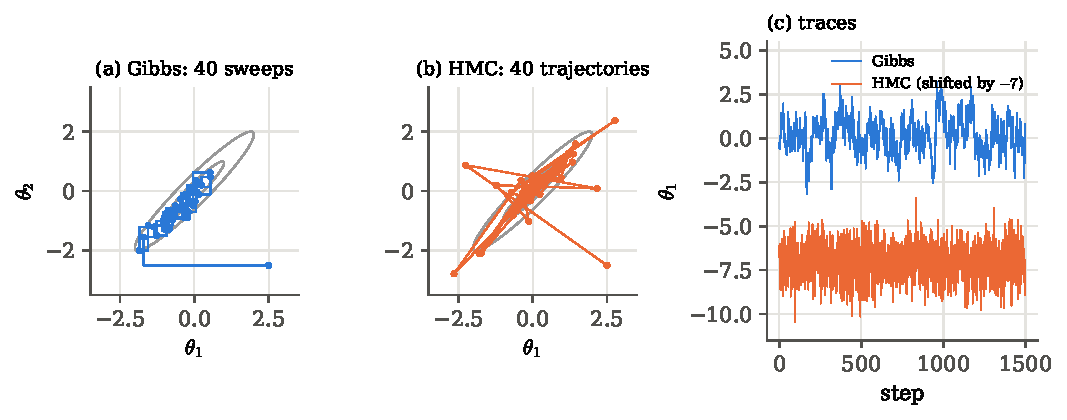
\includegraphics[width=\linewidth]{figures/ch09/gibbs_hmc.pdf}
\caption{Gibbs and Hamiltonian Monte Carlo on the Gaussian with correlation 0.95, both started at
$(2.5,-2.5)$. (a) Forty Gibbs sweeps: every move is parallel to an axis, so the ridge is climbed as
a staircase. (b) Forty HMC iterations (end points of the flights): each jumps across a large part
of the ellipse. (c) Traces of $\theta_1$: Gibbs (top) wanders slowly; HMC (bottom, shifted down by
7) decorrelates in about one iteration.}
\label{9b:fig:gibbs-hmc}
\end{figure}

\subsection{Ensembles of walkers, and the evidence}
\label{9b:sec:ensemble}

A different way to avoid tuning a proposal covariance is to let many walkers propose moves for
each other. In the affine-invariant ensemble sampler of \textcite{GoodmanWeare2010}, implemented
in \pyname{emcee} \parencite{ForemanMackey2013}, walker $k$ at $x_k$ picks another walker $x_j$ at
random and proposes the \emph{stretch move}
\begin{equation}
  y=x_j+\zeta\,(x_k-x_j),\qquad g(\zeta)\propto\frac{1}{\sqrt\zeta}\ \text{on }[1/a,a],
  \qquad \text{accept with }\min\Bigl(1,\zeta^{D-1}\frac{f(y)}{f(x_k)}\Bigr),
  \label{9b:eq:stretch}
\end{equation}
with $a=2$ by default. The candidate lies on the line through the two walkers, and the
\newterm{stretch factor} $\zeta$ says how far along it: $\zeta>1$ moves walker $k$ away from walker
$j$, $\zeta<1$ towards it. (Goodman and Weare call it $Z$; we write $\zeta$ because $Z$ is the
evidence and the partition function elsewhere in this chapter.)

\emph{Where $\zeta^{D-1}$ comes from.} Hold every other walker fixed, and measure positions from
$x_j$. Write the present position of walker $k$ in polar form, $x_k-x_j=r\,\omega$, with $r>0$ its
distance from $x_j$ and $\omega$ a unit vector. The stretch keeps $\omega$ and replaces $r$ by
$r'=\zeta r$: it is a one-dimensional move in $r$. In polar coordinates the volume element is
$r^{D-1}\dd r\,\dd\omega$ (the area of a sphere of radius $r$ times its thickness, as in
\eqref{9b:eq:shell}), so the target, as a density in $(r,\omega)$, is $f\,r^{D-1}$. Two things are
then needed. First, the proposal density of $r'$ given $r$, and the reverse, which must stretch by
$1/\zeta$ to come back:
\begin{align*}
  \frac{q(r\given r')}{q(r'\given r)}
  &\eqby{1}\frac{g(1/\zeta)/r'}{g(\zeta)/r}
   \eqby{2}\frac{g(1/\zeta)}{\zeta\,g(\zeta)}
   \eqby{3}\frac{\sqrt\zeta}{\zeta/\sqrt\zeta}=1 .
\end{align*}
\begin{explain}
  \item $r'=\zeta r$ with $\zeta\sim g$ has density $g(r'/r)/r$ in $r'$ (change of variable);
        the reverse move needs the factor $r/r'=1/\zeta$.
  \item $r'/r=\zeta$.
  \item With $g(\zeta)\propto1/\sqrt\zeta$: $g(1/\zeta)\propto\sqrt\zeta$ and
        $\zeta g(\zeta)\propto\sqrt\zeta$. The range $[1/a,a]$ is unchanged by $\zeta\to1/\zeta$,
        so the constants agree too.
\end{explain}
This is why $g$ is chosen $\propto1/\sqrt\zeta$: it is the choice that makes the stretch
symmetric in $r$, so no proposal factor is left. Second, the target ratio, in the same
coordinates:
\begin{equation*}
  \frac{f(y)\,(\zeta r)^{D-1}}{f(x_k)\,r^{D-1}}=\zeta^{D-1}\frac{f(y)}{f(x_k)} ,
\end{equation*}
which is the acceptance ratio of \eqref{9b:eq:stretch}. The factor $\zeta^{D-1}$ is the volume of
the larger sphere on which the stretched point sits.

\emph{Why linear correlations do not matter.} Apply a linear change of variables $x\to Ax+b$ to
every walker. Then $y-x_j=\zeta(x_k-x_j)$ becomes $A(y-x_j)=\zeta\,A(x_k-x_j)$: the same $\zeta$
produces the image of the same move. The transformed target differs from the original by the
constant factor $1/\abs{\det A}$, which cancels from the ratio. So every run in the new variables is
the image of a run in the old ones, with the same acceptances: a correlated Gaussian is sampled
exactly as efficiently as a round one, with no covariance to estimate. That is why \pyname{emcee} is so
popular in astrophysics. A curved banana is not a linear transformation of anything round, and
\cref{9b:sec:banana} showed \pyname{emcee} struggling on it, just like our walkers.

All these samplers share the property of \cref{9b:sec:ratios}: they never compute
the normalisation $Z$ of the target. That is their strength for parameter estimation and their
blind spot for model comparison, where the evidence is exactly what a Bayes factor needs
(\cref{ch:05}). \newterm{Nested sampling} \parencite{Skilling2006} attacks $Z$ directly. It
rewrites $Z=\int\Like\,p\,\dd\params$ as a one-dimensional integral $Z=\int_0^1\Like(X)\,\dd X$
over the prior mass $X$ enclosed by each likelihood contour, and estimates it with a set of
``live'' points that are repeatedly replaced by new points of higher likelihood, so that the
enclosed prior mass shrinks at each replacement by a factor whose distribution is known
\srcref{HobsonBMC}{§1.4.1, pp.~21--27}. Drawing the replacement point from the prior inside the
current contour is itself usually done with a short Markov chain. \Cref{ch:05} works through the
method; the posterior samples come as a by-product.

\begin{taxonomy}[Which sampler when]
\small
\begin{tabular}{@{}p{0.31\linewidth}p{0.62\linewidth}@{}}
random-walk Metropolis & any target you can evaluate; few parameters, or a good proposal
  covariance from a pilot run; no gradients needed\\[2pt]
Metropolis--Hastings with asymmetric $q$ & bounded parameters (log or logit steps with the
  Hastings factor); independence proposals from a good approximation\\[2pt]
Gibbs & conditionals easy to sample (conjugate hierarchical models); weakly correlated
  blocks\\[2pt]
Hamiltonian Monte Carlo & many parameters, smooth target, gradients available (automatic
  differentiation)\\[2pt]
ensemble (\texttt{emcee}) & moderate dimension, linear degeneracies, no gradients, little
  tuning\\[2pt]
tempering / nested sampling & several separated modes; the evidence $Z$ is wanted
\end{tabular}
\end{taxonomy}

Every example since \cref{9b:sec:biased} was chosen so that the answer was known in advance: a beta
posterior, a Gamma posterior, Gaussians, Onsager's solution. That made them verifications of the
machinery. The machinery earns its keep where no answer is known.

\begin{inpractice}[MCMC in cosmological parameter estimation]
\emph{Verification versus research.} Every chain above checked the sampler against an exact
answer. In research the posterior is unknown, and the sampler, with its diagnostics, is the
instrument that produces the published constraints.

\emph{What is run.} The workhorse for CMB and large-scale-structure likelihoods is still
Metropolis--Hastings, as in CosmoMC \parencite{LewisBridle2002} and its successor Cobaya: a
Gaussian proposal with the covariance of a previous run, scaled by about $2.4/\sqrt D$; ``fast''
nuisance parameters (foreground amplitudes, calibrations) updated more often than ``slow''
cosmological ones, because changing them does not require a new Boltzmann calculation; several
chains run in parallel, with $\hat R-1$ of a few hundredths or less as the stopping rule. \pyname{emcee}
is common in astrophysics for models with up to a few tens of parameters; HMC (through Stan, NumPyro
or similar) is used when the model is differentiable; nested samplers are run when the evidence is
needed. Lattice QCD runs on HMC, where it was invented \parencite{Duane1987}.

\emph{Laptop versus cluster.} Our chains are $10^4$--$10^5$ steps of targets that cost
microseconds. A Planck-like run evaluates a likelihood that needs a Boltzmann-code calculation of
order a second per step, for $10^5$ or more steps per chain and several chains: days on a cluster.
The CMB analysis that follows keeps the laptop scale by replacing the Boltzmann code with
a fast emulator; the statistics, the sampler and the diagnostics stay the same.
\end{inpractice}

Whichever sampler produced the chain, the same three questions are put to its output. Has it
forgotten where it started (burn-in and $\hat R$, \cref{9b:sec:burnin,9b:sec:rhat})? How many
independent draws does it hold ($\tau$ and the effective sample size, \cref{9b:sec:tau})? And is
the density it samples the one we meant, prior included (\cref{9b:sec:start-prior})? The samplers
differ only in how they propose; none of them changes the answers to these questions.

\begin{recap}
\begin{itemize}
  \item The unbiased random walker samples nothing; Metropolis--Hastings adds the bias. Propose
        $y\sim q(y\given x)$, accept with $\min(1,R_H)$,
        $R_H=f(y)q(x\given y)/[f(x)q(y\given x)]$; a refusal repeats the current point. Without
        the accept--reject step it is a random walk.
  \item Only ratios of $f$ enter, so the evidence of a posterior and the partition function of a
        Boltzmann weight cancel. Work with $\ln f$.
  \item Detailed balance fixes only the ratio of forward and backward acceptances; $\min(1,R_H)$ is
        the largest admissible choice (Peskun). Accepting with $\min(1,R^\beta)$ samples $f^\beta$.
        Asymmetric proposals need the Hastings factor, which is the Jacobian of the proposal (for
        $y=xe^{sZ}$ it is $y/x$); redrawing illegal proposals without it biases the chain.
  \item Step size: in $D$ dimensions the best round step is $2.38/\sqrt D$ target widths, with
        acceptance $\approx0.23$ (about $0.45$ in one dimension), and an independent draw every
        few $D$ steps. Correlated targets need a proposal shaped by the target's covariance; curved
        ones need a change of variables. A good acceptance rate does not imply a good chain.
  \item Burn-in ends when $\ln f$ fluctuates about its equilibrium level, $\simeq\ln f_{\max}-D/2$
        for a Gaussian, not at the peak. $\tau=1+2\sum\rho_k$ is estimated with a window (the full
        sum is identically zero); $\mathrm{ESS}=N/\tau$, $\mathrm{MCSE}=\mathrm{SD}\sqrt{\tau/N}$;
        thinning never improves an average.
  \item Several chains from overdispersed starts: $\hat R=\sqrt{\hat V/W}\to1$; in equilibrium
        $\hat R-1\simeq(1+1/M)\tau/2N$. $\hat R$ catches chains that disagree, never a mode that no
        chain found.
  \item The chain forgets its start (ergodicity); it never forgets the prior, which is part of the
        target. The prior's pull fades only with more data, as $1/\sqrt N$ posterior widths.
  \item Metropolis was invented for the canonical ensemble $e^{-H/kT}/Z$: it reproduces
        equipartition and the exponential energy law of the oscillator (a Boltzmann mixture of
        arcsine shells), Kramers' barrier-crossing rate in a double well, and Onsager's Ising
        solution on a lattice with $10^{308}$ states. MCMC time is not physical time.
  \item Relatives with the same decision rule: Gibbs (always accepted, slow on correlations),
        HMC (Hamiltonian flights plus momentum kicks, accepted with $e^{-\Delta H}$), affine-invariant
        ensembles (\texttt{emcee}); nested sampling computes the evidence that MCMC avoids.
\end{itemize}
\end{recap}
\providecommand{\NineCLineAhat}{}\renewcommand{\NineCLineAhat}{2.999}
\providecommand{\NineCLineBhat}{}\renewcommand{\NineCLineBhat}{1.9810}
\providecommand{\NineCLineSa}{}\renewcommand{\NineCLineSa}{0.0417}
\providecommand{\NineCLineSb}{}\renewcommand{\NineCLineSb}{0.0134}
\providecommand{\NineCLineRho}{}\renewcommand{\NineCLineRho}{-0.06}
\providecommand{\NineCLineAmc}{}\renewcommand{\NineCLineAmc}{2.999}
\providecommand{\NineCLineBmc}{}\renewcommand{\NineCLineBmc}{1.9811}
\providecommand{\NineCLineSamc}{}\renewcommand{\NineCLineSamc}{0.0416}
\providecommand{\NineCLineSbmc}{}\renewcommand{\NineCLineSbmc}{0.0136}
\providecommand{\NineCLineRhomc}{}\renewcommand{\NineCLineRhomc}{-0.05}
\providecommand{\NineCLineAcc}{}\renewcommand{\NineCLineAcc}{0.31}
\providecommand{\NineCLineRa}{}\renewcommand{\NineCLineRa}{1.0013}
\providecommand{\NineCLineRb}{}\renewcommand{\NineCLineRb}{1.0012}
\providecommand{\NineCLineTaua}{}\renewcommand{\NineCLineTaua}{6.7}
\providecommand{\NineCLineTaub}{}\renewcommand{\NineCLineTaub}{8.1}
\providecommand{\NineCLineESSa}{}\renewcommand{\NineCLineESSa}{6326}
\providecommand{\NineCLineESSb}{}\renewcommand{\NineCLineESSb}{5658}
\providecommand{\NineCLineNkept}{}\renewcommand{\NineCLineNkept}{45000}
\providecommand{\NineCLineChisq}{}\renewcommand{\NineCLineChisq}{33.0}
\providecommand{\NineCLineNdata}{}\renewcommand{\NineCLineNdata}{32}
\providecommand{\NineCLineNsteps}{}\renewcommand{\NineCLineNsteps}{10000}
\providecommand{\NineCLineBurn}{}\renewcommand{\NineCLineBurn}{1000}
\providecommand{\NineCLineXrms}{}\renewcommand{\NineCLineXrms}{2.99}
\providecommand{\NineCLineSaFloor}{}\renewcommand{\NineCLineSaFloor}{0.0416}
\providecommand{\NineCLineMCSEb}{}\renewcommand{\NineCLineMCSEb}{0.00018}
\providecommand{\NineCLineAem}{}\renewcommand{\NineCLineAem}{2.998}
\providecommand{\NineCLineSaem}{}\renewcommand{\NineCLineSaem}{0.0422}
\providecommand{\NineCLineBem}{}\renewcommand{\NineCLineBem}{1.9804}
\providecommand{\NineCLineSbem}{}\renewcommand{\NineCLineSbem}{0.0129}
\providecommand{\NineCLineSAmc}{}\renewcommand{\NineCLineSAmc}{2.976}
\providecommand{\NineCLineSSamc}{}\renewcommand{\NineCLineSSamc}{0.0516}
\providecommand{\NineCLineSBmc}{}\renewcommand{\NineCLineSBmc}{1.9805}
\providecommand{\NineCLineSSbmc}{}\renewcommand{\NineCLineSSbmc}{0.0171}
\providecommand{\NineCLineSSigmc}{}\renewcommand{\NineCLineSSigmc}{0.287}
\providecommand{\NineCLineSSSigmc}{}\renewcommand{\NineCLineSSSigmc}{0.038}
\providecommand{\NineCLineSAex}{}\renewcommand{\NineCLineSAex}{2.977}
\providecommand{\NineCLineSSaex}{}\renewcommand{\NineCLineSSaex}{0.0514}
\providecommand{\NineCLineSBex}{}\renewcommand{\NineCLineSBex}{1.9805}
\providecommand{\NineCLineSSbex}{}\renewcommand{\NineCLineSSbex}{0.0172}
\providecommand{\NineCLineSnu}{}\renewcommand{\NineCLineSnu}{29}
\providecommand{\NineCLineSrms}{}\renewcommand{\NineCLineSrms}{0.276}
\providecommand{\NineCLineSAcc}{}\renewcommand{\NineCLineSAcc}{0.37}
\providecommand{\NineCLineSRmax}{}\renewcommand{\NineCLineSRmax}{1.0013}
\providecommand{\NineCLinePooled}{}\renewcommand{\NineCLinePooled}{0.255}
\providecommand{\NineCLineKSaMed}{}\renewcommand{\NineCLineKSaMed}{0.0420}
\providecommand{\NineCLineKSaLo}{}\renewcommand{\NineCLineKSaLo}{0.0416}
\providecommand{\NineCLineKSaHi}{}\renewcommand{\NineCLineKSaHi}{0.0432}
\providecommand{\NineCLineKSbMed}{}\renewcommand{\NineCLineKSbMed}{0.0143}
\providecommand{\NineCLineKSbLo}{}\renewcommand{\NineCLineKSbLo}{0.0126}
\providecommand{\NineCLineKSbHi}{}\renewcommand{\NineCLineKSbHi}{0.0165}
\providecommand{\NineCLineKPadSaPct}{}\renewcommand{\NineCLineKPadSaPct}{99}
\providecommand{\NineCLineKPadSbPct}{}\renewcommand{\NineCLineKPadSbPct}{23}
\providecommand{\NineCLineSSaMed}{}\renewcommand{\NineCLineSSaMed}{0.0477}
\providecommand{\NineCLineSSaLo}{}\renewcommand{\NineCLineSSaLo}{0.0412}
\providecommand{\NineCLineSSaHi}{}\renewcommand{\NineCLineSSaHi}{0.0545}
\providecommand{\NineCLineSSbMed}{}\renewcommand{\NineCLineSSbMed}{0.0160}
\providecommand{\NineCLineSSbLo}{}\renewcommand{\NineCLineSSbLo}{0.0133}
\providecommand{\NineCLineSSbHi}{}\renewcommand{\NineCLineSSbHi}{0.0193}
\providecommand{\NineCLineSPadSaPct}{}\renewcommand{\NineCLineSPadSaPct}{46}
\providecommand{\NineCLineSPadSbPct}{}\renewcommand{\NineCLineSPadSbPct}{13}
\providecommand{\NineCLineNrep}{}\renewcommand{\NineCLineNrep}{20000}
\providecommand{\NineCLineShift}{}\renewcommand{\NineCLineShift}{10}
\providecommand{\NineCLineRhoShift}{}\renewcommand{\NineCLineRhoShift}{-0.955}
\providecommand{\NineCLineRhoCent}{}\renewcommand{\NineCLineRhoCent}{-0.014}
\providecommand{\NineCLineTauCent}{}\renewcommand{\NineCLineTauCent}{5.7}
\providecommand{\NineCLineTauShift}{}\renewcommand{\NineCLineTauShift}{342}
\providecommand{\NineCLineAccCent}{}\renewcommand{\NineCLineAccCent}{0.30}
\providecommand{\NineCLineAccShift}{}\renewcommand{\NineCLineAccShift}{0.12}
\providecommand{\NineCLineSaShift}{}\renewcommand{\NineCLineSaShift}{0.141}
\providecommand{\NineCLineSaCent}{}\renewcommand{\NineCLineSaCent}{0.0416}
\providecommand{\NineCExpN}{}\renewcommand{\NineCExpN}{15}
\providecommand{\NineCExpAtrue}{}\renewcommand{\NineCExpAtrue}{100}
\providecommand{\NineCExpTautrue}{}\renewcommand{\NineCExpTautrue}{4}
\providecommand{\NineCExpSigtrue}{}\renewcommand{\NineCExpSigtrue}{6}
\providecommand{\NineCExpSigWrong}{}\renewcommand{\NineCExpSigWrong}{3}
\providecommand{\NineCExpAhat}{}\renewcommand{\NineCExpAhat}{97.0}
\providecommand{\NineCExpTauhat}{}\renewcommand{\NineCExpTauhat}{4.31}
\providecommand{\NineCExpSaLap}{}\renewcommand{\NineCExpSaLap}{4.7}
\providecommand{\NineCExpStLap}{}\renewcommand{\NineCExpStLap}{0.34}
\providecommand{\NineCExpRhoLap}{}\renewcommand{\NineCExpRhoLap}{-0.63}
\providecommand{\NineCExpTauMean}{}\renewcommand{\NineCExpTauMean}{4.35}
\providecommand{\NineCExpTauSd}{}\renewcommand{\NineCExpTauSd}{0.34}
\providecommand{\NineCExpTauSkew}{}\renewcommand{\NineCExpTauSkew}{0.26}
\providecommand{\NineCExpTauMeanMC}{}\renewcommand{\NineCExpTauMeanMC}{4.35}
\providecommand{\NineCExpTauSdMC}{}\renewcommand{\NineCExpTauSdMC}{0.34}
\providecommand{\NineCExpAMeanMC}{}\renewcommand{\NineCExpAMeanMC}{96.8}
\providecommand{\NineCExpASdMC}{}\renewcommand{\NineCExpASdMC}{4.7}
\providecommand{\NineCExpRhoMC}{}\renewcommand{\NineCExpRhoMC}{-0.63}
\providecommand{\NineCExpTauSkewMC}{}\renewcommand{\NineCExpTauSkewMC}{0.32}
\providecommand{\NineCExpAccK}{}\renewcommand{\NineCExpAccK}{0.36}
\providecommand{\NineCExpAccThree}{}\renewcommand{\NineCExpAccThree}{0.33}
\providecommand{\NineCExpRmax}{}\renewcommand{\NineCExpRmax}{1.0009}
\providecommand{\NineCExpTauMeanMarg}{}\renewcommand{\NineCExpTauMeanMarg}{4.36}
\providecommand{\NineCExpTauSdMarg}{}\renewcommand{\NineCExpTauSdMarg}{0.39}
\providecommand{\NineCExpTauMeanChain}{}\renewcommand{\NineCExpTauMeanChain}{4.36}
\providecommand{\NineCExpTauSdChain}{}\renewcommand{\NineCExpTauSdChain}{0.39}
\providecommand{\NineCExpTauSdWrong}{}\renewcommand{\NineCExpTauSdWrong}{0.17}
\providecommand{\NineCExpSigMed}{}\renewcommand{\NineCExpSigMed}{6.4}
\providecommand{\NineCExpSigLo}{}\renewcommand{\NineCExpSigLo}{5.4}
\providecommand{\NineCExpSigHi}{}\renewcommand{\NineCExpSigHi}{8.0}
\providecommand{\NineCExpChiMin}{}\renewcommand{\NineCExpChiMin}{14.2}
\providecommand{\NineCExpNsteps}{}\renewcommand{\NineCExpNsteps}{20000}
\providecommand{\NineCExpBurn}{}\renewcommand{\NineCExpBurn}{2000}
\providecommand{\NineCHypAzero}{}\renewcommand{\NineCHypAzero}{3.276}
\providecommand{\NineCHypSAzero}{}\renewcommand{\NineCHypSAzero}{0.066}
\providecommand{\NineCHypBzero}{}\renewcommand{\NineCHypBzero}{1.864}
\providecommand{\NineCHypSBzero}{}\renewcommand{\NineCHypSBzero}{0.024}
\providecommand{\NineCHypKtwo}{}\renewcommand{\NineCHypKtwo}{4.340\times10^{17}}
\providecommand{\NineCHypLnKtwo}{}\renewcommand{\NineCHypLnKtwo}{40.6}
\providecommand{\NineCHypKone}{}\renewcommand{\NineCHypKone}{0.59}
\providecommand{\NineCHypLnKone}{}\renewcommand{\NineCHypLnKone}{-0.53}
\providecommand{\NineCHypWup}{}\renewcommand{\NineCHypWup}{1.00}
\providecommand{\NineCHypWlow}{}\renewcommand{\NineCHypWlow}{0.0031}
\providecommand{\NineCHypDpeak}{}\renewcommand{\NineCHypDpeak}{7.2}
\providecommand{\NineCHypAlow}{}\renewcommand{\NineCHypAlow}{3.71}
\providecommand{\NineCHypBlow}{}\renewcommand{\NineCHypBlow}{1.61}
\providecommand{\NineCHypChainsBoth}{}\renewcommand{\NineCHypChainsBoth}{0}
\providecommand{\NineCHypChainsN}{}\renewcommand{\NineCHypChainsN}{6}
\providecommand{\NineCHypChiZero}{}\renewcommand{\NineCHypChiZero}{158}
\providecommand{\NineCLikeMeanFactor}{}\renewcommand{\NineCLikeMeanFactor}{1.571}
\providecommand{\NineCLikeModeFactor}{}\renewcommand{\NineCLikeModeFactor}{0.818}
\providecommand{\NineCHLcheck}{}\renewcommand{\NineCHLcheck}{1.500\times10^{-8}}
\providecommand{\NineCHLbiasS}{}\renewcommand{\NineCHLbiasS}{0.00175}
\providecommand{\NineCHLrmsS}{}\renewcommand{\NineCHLrmsS}{0.00194}
\providecommand{\NineCHLrmsSHund}{}\renewcommand{\NineCHLrmsSHund}{0.0187}
\providecommand{\NineCHLbiasQ}{}\renewcommand{\NineCHLbiasQ}{8.770\times10^{-4}}
\providecommand{\NineCHLrmsQ}{}\renewcommand{\NineCHLrmsQ}{9.700\times10^{-4}}
\providecommand{\NineCHLrmsQHund}{}\renewcommand{\NineCHLrmsQHund}{0.00936}
\providecommand{\NineCHLbiasD}{}\renewcommand{\NineCHLbiasD}{3.890\times10^{-4}}
\providecommand{\NineCHLrmsD}{}\renewcommand{\NineCHLrmsD}{5.690\times10^{-4}}
\providecommand{\NineCHLrmsDHund}{}\renewcommand{\NineCHLrmsDHund}{0.00546}
\providecommand{\NineCHLbiasLN}{}\renewcommand{\NineCHLbiasLN}{4.380\times10^{-4}}
\providecommand{\NineCHLrmsLN}{}\renewcommand{\NineCHLrmsLN}{4.850\times10^{-4}}
\providecommand{\NineCHLrmsLNHund}{}\renewcommand{\NineCHLrmsLNHund}{0.00468}
\providecommand{\NineCHLbiasWMAP}{}\renewcommand{\NineCHLbiasWMAP}{5.500\times10^{-8}}
\providecommand{\NineCHLrmsWMAP}{}\renewcommand{\NineCHLrmsWMAP}{4.480\times10^{-6}}
\providecommand{\NineCHLrmsWMAPHund}{}\renewcommand{\NineCHLrmsWMAPHund}{1.350\times10^{-4}}
\providecommand{\NineCHLbiasCube}{}\renewcommand{\NineCHLbiasCube}{6.430\times10^{-8}}
\providecommand{\NineCHLrmsCube}{}\renewcommand{\NineCHLrmsCube}{7.510\times10^{-7}}
\providecommand{\NineCHLrmsCubeHund}{}\renewcommand{\NineCHLrmsCubeHund}{2.330\times10^{-5}}
\providecommand{\NineCHLlref}{}\renewcommand{\NineCHLlref}{1022}
\providecommand{\NineCHLlrefHund}{}\renewcommand{\NineCHLlrefHund}{102}
\providecommand{\NineCHLnsim}{}\renewcommand{\NineCHLnsim}{10000}
\providecommand{\NineCHLQoverL}{}\renewcommand{\NineCHLQoverL}{0.90}
\providecommand{\NineCHLSoverL}{}\renewcommand{\NineCHLSoverL}{1.79}
\providecommand{\NineCHLDoverL}{}\renewcommand{\NineCHLDoverL}{0.40}
\providecommand{\NineCHLpubRmsS}{}\renewcommand{\NineCHLpubRmsS}{0.002}
\providecommand{\NineCHLpubBiasS}{}\renewcommand{\NineCHLpubBiasS}{0.0018}
\providecommand{\NineCHLpubRmsQ}{}\renewcommand{\NineCHLpubRmsQ}{0.001}
\providecommand{\NineCHLpubBiasQ}{}\renewcommand{\NineCHLpubBiasQ}{9.100\times10^{-4}}
\providecommand{\NineCHLpubRmsD}{}\renewcommand{\NineCHLpubRmsD}{5.800\times10^{-4}}
\providecommand{\NineCHLpubBiasD}{}\renewcommand{\NineCHLpubBiasD}{4.000\times10^{-4}}
\providecommand{\NineCHLpubRmsWMAP}{}\renewcommand{\NineCHLpubRmsWMAP}{5.000\times10^{-6}}
\providecommand{\NineCHLpubRmsCube}{}\renewcommand{\NineCHLpubRmsCube}{1.400\times10^{-6}}
\providecommand{\NineCEmuBuildCalls}{}\renewcommand{\NineCEmuBuildCalls}{73}
\providecommand{\NineCEmuSigLnAs}{}\renewcommand{\NineCEmuSigLnAs}{0.01674}
\providecommand{\NineCEmuSigNs}{}\renewcommand{\NineCEmuSigNs}{0.005293}
\providecommand{\NineCEmuSigHzero}{}\renewcommand{\NineCEmuSigHzero}{0.9365}
\providecommand{\NineCEmuSigOmb}{}\renewcommand{\NineCEmuSigOmb}{0.0002014}
\providecommand{\NineCEmuSigOmc}{}\renewcommand{\NineCEmuSigOmc}{0.002157}
\providecommand{\NineCEmuSigTau}{}\renewcommand{\NineCEmuSigTau}{0.008346}
\providecommand{\NineCEmuSigLnAsTwo}{}\renewcommand{\NineCEmuSigLnAsTwo}{0.0018}
\providecommand{\NineCEmuSigNsTwo}{}\renewcommand{\NineCEmuSigNsTwo}{0.0026}
\providecommand{\NineCEmuRhoTwo}{}\renewcommand{\NineCEmuRhoTwo}{-0.73}
\providecommand{\NineCEmuRhoSix}{}\renewcommand{\NineCEmuRhoSix}{-0.15}
\providecommand{\NineCEmuMedLinC}{}\renewcommand{\NineCEmuMedLinC}{0.0535}
\providecommand{\NineCEmuMaxLinC}{}\renewcommand{\NineCEmuMaxLinC}{2}
\providecommand{\NineCEmuCutFiveLinC}{}\renewcommand{\NineCEmuCutFiveLinC}{35.5}
\providecommand{\NineCEmuCutOneLinC}{}\renewcommand{\NineCEmuCutOneLinC}{0.054}
\providecommand{\NineCEmuMedLin}{}\renewcommand{\NineCEmuMedLin}{0.0484}
\providecommand{\NineCEmuMaxLin}{}\renewcommand{\NineCEmuMaxLin}{1.98}
\providecommand{\NineCEmuCutFiveLin}{}\renewcommand{\NineCEmuCutFiveLin}{33}
\providecommand{\NineCEmuCutOneLin}{}\renewcommand{\NineCEmuCutOneLin}{0.0485}
\providecommand{\NineCEmuMedQuad}{}\renewcommand{\NineCEmuMedQuad}{6.550\times10^{-4}}
\providecommand{\NineCEmuMaxQuad}{}\renewcommand{\NineCEmuMaxQuad}{0.0964}
\providecommand{\NineCEmuCutFiveQuad}{}\renewcommand{\NineCEmuCutFiveQuad}{0.515}
\providecommand{\NineCEmuCutOneQuad}{}\renewcommand{\NineCEmuCutOneQuad}{5.290\times10^{-5}}
\providecommand{\NineCEmuTwoWorst}{}\renewcommand{\NineCEmuTwoWorst}{2.890\times10^{-5}}
\providecommand{\NineCEmuNrand}{}\renewcommand{\NineCEmuNrand}{40}
\providecommand{\NineCEmuMaxDist}{}\renewcommand{\NineCEmuMaxDist}{7.3}
\providecommand{\NineCEmuFsky}{}\renewcommand{\NineCEmuFsky}{0.57}
\providecommand{\NineCEmuSigTauPrior}{}\renewcommand{\NineCEmuSigTauPrior}{0.0086}
\providecommand{\NineCEmuHAA}{}\renewcommand{\NineCEmuHAA}{0.041}
\providecommand{\NineCEmuHnn}{}\renewcommand{\NineCEmuHnn}{0.08}
\providecommand{\NineCEmuDnThousand}{}\renewcommand{\NineCEmuDnThousand}{0.55}
\providecommand{\NineCEmuDnTen}{}\renewcommand{\NineCEmuDnTen}{-3.61}
\providecommand{\NineCEmuDtauHigh}{}\renewcommand{\NineCEmuDtauHigh}{-2.00}
\providecommand{\NineCEmuMinutes}{}\renewcommand{\NineCEmuMinutes}{1.2}
\providecommand{\NineCEmuTemu}{}\renewcommand{\NineCEmuTemu}{54}
\providecommand{\NineCEmuTcamb}{}\renewcommand{\NineCEmuTcamb}{0.9}
\providecommand{\NineCEmuSpeedup}{}\renewcommand{\NineCEmuSpeedup}{16496}
\providecommand{\NineCToyLmax}{}\renewcommand{\NineCToyLmax}{601}
\providecommand{\NineCToyNbins}{}\renewcommand{\NineCToyNbins}{30}
\providecommand{\NineCToyNsims}{}\renewcommand{\NineCToyNsims}{2000}
\providecommand{\NineCToyHartlap}{}\renewcommand{\NineCToyHartlap}{0.9845}
\providecommand{\NineCToyFsky}{}\renewcommand{\NineCToyFsky}{0.658}
\providecommand{\NineCToyFullA}{}\renewcommand{\NineCToyFullA}{3.0446}
\providecommand{\NineCToyFullSA}{}\renewcommand{\NineCToyFullSA}{0.0029}
\providecommand{\NineCToyFullN}{}\renewcommand{\NineCToyFullN}{0.9649}
\providecommand{\NineCToyFullSN}{}\renewcommand{\NineCToyFullSN}{0.0050}
\providecommand{\NineCToyFullRho}{}\renewcommand{\NineCToyFullRho}{0.59}
\providecommand{\NineCToyFullAcc}{}\renewcommand{\NineCToyFullAcc}{0.36}
\providecommand{\NineCToyFullRhat}{}\renewcommand{\NineCToyFullRhat}{1.0013}
\providecommand{\NineCToyFullTau}{}\renewcommand{\NineCToyFullTau}{8.4}
\providecommand{\NineCToyFullESS}{}\renewcommand{\NineCToyFullESS}{9471}
\providecommand{\NineCToyFullSec}{}\renewcommand{\NineCToyFullSec}{1}
\providecommand{\NineCToyFullFSA}{}\renewcommand{\NineCToyFullFSA}{0.0029}
\providecommand{\NineCToyFullFSN}{}\renewcommand{\NineCToyFullFSN}{0.0049}
\providecommand{\NineCToyFullFRho}{}\renewcommand{\NineCToyFullFRho}{0.59}
\providecommand{\NineCToyNoisyA}{}\renewcommand{\NineCToyNoisyA}{3.0400}
\providecommand{\NineCToyNoisySA}{}\renewcommand{\NineCToyNoisySA}{0.0063}
\providecommand{\NineCToyNoisyN}{}\renewcommand{\NineCToyNoisyN}{0.9604}
\providecommand{\NineCToyNoisySN}{}\renewcommand{\NineCToyNoisySN}{0.0072}
\providecommand{\NineCToyNoisyRho}{}\renewcommand{\NineCToyNoisyRho}{0.83}
\providecommand{\NineCToyNoisyAcc}{}\renewcommand{\NineCToyNoisyAcc}{0.36}
\providecommand{\NineCToyNoisyRhat}{}\renewcommand{\NineCToyNoisyRhat}{1.0005}
\providecommand{\NineCToyNoisyTau}{}\renewcommand{\NineCToyNoisyTau}{6.4}
\providecommand{\NineCToyNoisyESS}{}\renewcommand{\NineCToyNoisyESS}{10259}
\providecommand{\NineCToyNoisySec}{}\renewcommand{\NineCToyNoisySec}{1}
\providecommand{\NineCToyNoisyFSA}{}\renewcommand{\NineCToyNoisyFSA}{0.0063}
\providecommand{\NineCToyNoisyFSN}{}\renewcommand{\NineCToyNoisyFSN}{0.0072}
\providecommand{\NineCToyNoisyFRho}{}\renewcommand{\NineCToyNoisyFRho}{0.83}
\providecommand{\NineCToyMaskA}{}\renewcommand{\NineCToyMaskA}{3.0519}
\providecommand{\NineCToyMaskSA}{}\renewcommand{\NineCToyMaskSA}{0.0083}
\providecommand{\NineCToyMaskN}{}\renewcommand{\NineCToyMaskN}{0.9698}
\providecommand{\NineCToyMaskSN}{}\renewcommand{\NineCToyMaskSN}{0.0095}
\providecommand{\NineCToyMaskRho}{}\renewcommand{\NineCToyMaskRho}{0.83}
\providecommand{\NineCToyMaskAcc}{}\renewcommand{\NineCToyMaskAcc}{0.36}
\providecommand{\NineCToyMaskRhat}{}\renewcommand{\NineCToyMaskRhat}{1.0006}
\providecommand{\NineCToyMaskTau}{}\renewcommand{\NineCToyMaskTau}{8.0}
\providecommand{\NineCToyMaskESS}{}\renewcommand{\NineCToyMaskESS}{9336}
\providecommand{\NineCToyMaskSec}{}\renewcommand{\NineCToyMaskSec}{1}
\providecommand{\NineCToyMaskFSA}{}\renewcommand{\NineCToyMaskFSA}{0.0082}
\providecommand{\NineCToyMaskFSN}{}\renewcommand{\NineCToyMaskFSN}{0.0094}
\providecommand{\NineCToyMaskFRho}{}\renewcommand{\NineCToyMaskFRho}{0.83}
\providecommand{\NineCToyQuadA}{}\renewcommand{\NineCToyQuadA}{3.0457}
\providecommand{\NineCToyQuadSA}{}\renewcommand{\NineCToyQuadSA}{0.0029}
\providecommand{\NineCToyQuadN}{}\renewcommand{\NineCToyQuadN}{0.9592}
\providecommand{\NineCToyQuadSN}{}\renewcommand{\NineCToyQuadSN}{0.0049}
\providecommand{\NineCToyQuadRho}{}\renewcommand{\NineCToyQuadRho}{0.58}
\providecommand{\NineCToyQuadAcc}{}\renewcommand{\NineCToyQuadAcc}{0.36}
\providecommand{\NineCToyQuadRhat}{}\renewcommand{\NineCToyQuadRhat}{1.0009}
\providecommand{\NineCToyQuadTau}{}\renewcommand{\NineCToyQuadTau}{6.8}
\providecommand{\NineCToyQuadESS}{}\renewcommand{\NineCToyQuadESS}{10100}
\providecommand{\NineCToyQuadSec}{}\renewcommand{\NineCToyQuadSec}{1}
\providecommand{\NineCToyFidA}{}\renewcommand{\NineCToyFidA}{3.0445}
\providecommand{\NineCToyFidSA}{}\renewcommand{\NineCToyFidSA}{0.0029}
\providecommand{\NineCToyFidN}{}\renewcommand{\NineCToyFidN}{0.9650}
\providecommand{\NineCToyFidSN}{}\renewcommand{\NineCToyFidSN}{0.0049}
\providecommand{\NineCToyFidRho}{}\renewcommand{\NineCToyFidRho}{0.58}
\providecommand{\NineCToyFidAcc}{}\renewcommand{\NineCToyFidAcc}{0.36}
\providecommand{\NineCToyFidRhat}{}\renewcommand{\NineCToyFidRhat}{1.0007}
\providecommand{\NineCToyFidTau}{}\renewcommand{\NineCToyFidTau}{8.1}
\providecommand{\NineCToyFidESS}{}\renewcommand{\NineCToyFidESS}{9760}
\providecommand{\NineCToyFidSec}{}\renewcommand{\NineCToyFidSec}{1}
\providecommand{\NineCToyFullPullN}{}\renewcommand{\NineCToyFullPullN}{+0.0}
\providecommand{\NineCToyFullPullA}{}\renewcommand{\NineCToyFullPullA}{+0.0}
\providecommand{\NineCToyNoisyPullN}{}\renewcommand{\NineCToyNoisyPullN}{-0.6}
\providecommand{\NineCToyNoisyPullA}{}\renewcommand{\NineCToyNoisyPullA}{-0.7}
\providecommand{\NineCToyMaskPullN}{}\renewcommand{\NineCToyMaskPullN}{+0.5}
\providecommand{\NineCToyMaskPullA}{}\renewcommand{\NineCToyMaskPullA}{+0.9}
\providecommand{\NineCToyQuadPullN}{}\renewcommand{\NineCToyQuadPullN}{-1.2}
\providecommand{\NineCToyQuadPullA}{}\renewcommand{\NineCToyQuadPullA}{+0.4}
\providecommand{\NineCToyFidPullN}{}\renewcommand{\NineCToyFidPullN}{+0.0}
\providecommand{\NineCToyFidPullA}{}\renewcommand{\NineCToyFidPullA}{+0.0}
\providecommand{\NineCToyTruthA}{}\renewcommand{\NineCToyTruthA}{3.0445}
\providecommand{\NineCToyTruthN}{}\renewcommand{\NineCToyTruthN}{0.9649}
\providecommand{\NineCToyNch}{}\renewcommand{\NineCToyNch}{4}
\providecommand{\NineCToyNst}{}\renewcommand{\NineCToyNst}{20000}
\providecommand{\NineCToyBurn}{}\renewcommand{\NineCToyBurn}{2000}
\providecommand{\NineCToyShiftQ}{}\renewcommand{\NineCToyShiftQ}{-1.15}
\providecommand{\NineCToyShiftF}{}\renewcommand{\NineCToyShiftF}{+0.01}
\providecommand{\NineCToyEmA}{}\renewcommand{\NineCToyEmA}{3.0518}
\providecommand{\NineCToyEmSA}{}\renewcommand{\NineCToyEmSA}{0.0083}
\providecommand{\NineCToyEmN}{}\renewcommand{\NineCToyEmN}{0.9698}
\providecommand{\NineCToyEmSN}{}\renewcommand{\NineCToyEmSN}{0.0093}
\providecommand{\NineCToyGdNlo}{}\renewcommand{\NineCToyGdNlo}{0.9603}
\providecommand{\NineCToyGdNhi}{}\renewcommand{\NineCToyGdNhi}{0.9792}
\providecommand{\NineCToyOurNlo}{}\renewcommand{\NineCToyOurNlo}{0.9603}
\providecommand{\NineCToyOurNhi}{}\renewcommand{\NineCToyOurNhi}{0.9792}
\providecommand{\NineCToyEnsN}{}\renewcommand{\NineCToyEnsN}{500}
\providecommand{\NineCToyEnsQmean}{}\renewcommand{\NineCToyEnsQmean}{-1.25}
\providecommand{\NineCToyEnsQsd}{}\renewcommand{\NineCToyEnsQsd}{0.17}
\providecommand{\NineCToyEnsFmean}{}\renewcommand{\NineCToyEnsFmean}{-0.000}
\providecommand{\NineCToyEnsFsd}{}\renewcommand{\NineCToyEnsFsd}{0.009}
\providecommand{\NineCToyEnsQAmean}{}\renewcommand{\NineCToyEnsQAmean}{+0.38}
\providecommand{\NineCToyEnsExactBias}{}\renewcommand{\NineCToyEnsExactBias}{+0.03}
\providecommand{\NineCToyEnsExactSd}{}\renewcommand{\NineCToyEnsExactSd}{1.05}
\providecommand{\NineCToyMinutes}{}\renewcommand{\NineCToyMinutes}{0.2}
\providecommand{\NineCPlFsky}{}\renewcommand{\NineCPlFsky}{0.57}
\providecommand{\NineCPlSigTau}{}\renewcommand{\NineCPlSigTau}{0.0086}
\providecommand{\NineCPlTauObs}{}\renewcommand{\NineCPlTauObs}{0.0714}
\providecommand{\NineCPlTauTrue}{}\renewcommand{\NineCPlTauTrue}{0.0544}
\providecommand{\NineCPlLmax}{}\renewcommand{\NineCPlLmax}{2500}
\providecommand{\NineCPlPubRho}{}\renewcommand{\NineCPlPubRho}{+0.03}
\providecommand{\NineCPlPubCovSA}{}\renewcommand{\NineCPlPubCovSA}{0.0164}
\providecommand{\NineCPlPubCovSN}{}\renewcommand{\NineCPlPubCovSN}{0.0057}
\providecommand{\NineCPlTwoA}{}\renewcommand{\NineCPlTwoA}{3.0441}
\providecommand{\NineCPlTwoSA}{}\renewcommand{\NineCPlTwoSA}{0.0018}
\providecommand{\NineCPlTwoN}{}\renewcommand{\NineCPlTwoN}{0.9664}
\providecommand{\NineCPlTwoSN}{}\renewcommand{\NineCPlTwoSN}{0.0026}
\providecommand{\NineCPlTwoRho}{}\renewcommand{\NineCPlTwoRho}{-0.73}
\providecommand{\NineCPlTwoAcc}{}\renewcommand{\NineCPlTwoAcc}{0.35}
\providecommand{\NineCPlTwoRhat}{}\renewcommand{\NineCPlTwoRhat}{1.0001}
\providecommand{\NineCPlTwoTau}{}\renewcommand{\NineCPlTwoTau}{8}
\providecommand{\NineCPlTwoSec}{}\renewcommand{\NineCPlTwoSec}{5}
\providecommand{\NineCPlTwoFSA}{}\renewcommand{\NineCPlTwoFSA}{0.0018}
\providecommand{\NineCPlTwoFSN}{}\renewcommand{\NineCPlTwoFSN}{0.0026}
\providecommand{\NineCPlTwoFRho}{}\renewcommand{\NineCPlTwoFRho}{-0.73}
\providecommand{\NineCPlThreeA}{}\renewcommand{\NineCPlThreeA}{3.0776}
\providecommand{\NineCPlThreeSA}{}\renewcommand{\NineCPlThreeSA}{0.0164}
\providecommand{\NineCPlThreeN}{}\renewcommand{\NineCPlThreeN}{0.9665}
\providecommand{\NineCPlThreeSN}{}\renewcommand{\NineCPlThreeSN}{0.0026}
\providecommand{\NineCPlThreeRho}{}\renewcommand{\NineCPlThreeRho}{-0.06}
\providecommand{\NineCPlThreeAcc}{}\renewcommand{\NineCPlThreeAcc}{0.32}
\providecommand{\NineCPlThreeRhat}{}\renewcommand{\NineCPlThreeRhat}{1.0004}
\providecommand{\NineCPlThreeTau}{}\renewcommand{\NineCPlThreeTau}{10}
\providecommand{\NineCPlThreeSec}{}\renewcommand{\NineCPlThreeSec}{5}
\providecommand{\NineCPlThreeFSA}{}\renewcommand{\NineCPlThreeFSA}{0.0165}
\providecommand{\NineCPlThreeFSN}{}\renewcommand{\NineCPlThreeFSN}{0.0026}
\providecommand{\NineCPlThreeFRho}{}\renewcommand{\NineCPlThreeFRho}{-0.06}
\providecommand{\NineCPlThreeT}{}\renewcommand{\NineCPlThreeT}{0.0712}
\providecommand{\NineCPlThreeST}{}\renewcommand{\NineCPlThreeST}{0.0082}
\providecommand{\NineCPlThreeRhoAT}{}\renewcommand{\NineCPlThreeRhoAT}{+0.99}
\providecommand{\NineCPlSixA}{}\renewcommand{\NineCPlSixA}{3.0794}
\providecommand{\NineCPlSixSA}{}\renewcommand{\NineCPlSixSA}{0.017}
\providecommand{\NineCPlSixN}{}\renewcommand{\NineCPlSixN}{0.9642}
\providecommand{\NineCPlSixSN}{}\renewcommand{\NineCPlSixSN}{0.0053}
\providecommand{\NineCPlSixRho}{}\renewcommand{\NineCPlSixRho}{-0.14}
\providecommand{\NineCPlSixAcc}{}\renewcommand{\NineCPlSixAcc}{0.28}
\providecommand{\NineCPlSixRhat}{}\renewcommand{\NineCPlSixRhat}{1.0006}
\providecommand{\NineCPlSixTau}{}\renewcommand{\NineCPlSixTau}{23}
\providecommand{\NineCPlSixSec}{}\renewcommand{\NineCPlSixSec}{12}
\providecommand{\NineCPlSixFSA}{}\renewcommand{\NineCPlSixFSA}{0.0167}
\providecommand{\NineCPlSixFSN}{}\renewcommand{\NineCPlSixFSN}{0.0053}
\providecommand{\NineCPlSixFRho}{}\renewcommand{\NineCPlSixFRho}{-0.15}
\providecommand{\NineCPlSixT}{}\renewcommand{\NineCPlSixT}{0.0705}
\providecommand{\NineCPlSixST}{}\renewcommand{\NineCPlSixST}{0.0083}
\providecommand{\NineCPlSixRhoAT}{}\renewcommand{\NineCPlSixRhoAT}{+0.94}
\providecommand{\NineCPlSixMA}{}\renewcommand{\NineCPlSixMA}{3.0794}
\providecommand{\NineCPlSixMN}{}\renewcommand{\NineCPlSixMN}{0.9642}
\providecommand{\NineCPlSixMH}{}\renewcommand{\NineCPlSixMH}{67.058}
\providecommand{\NineCPlSixSH}{}\renewcommand{\NineCPlSixSH}{0.93}
\providecommand{\NineCPlSixMB}{}\renewcommand{\NineCPlSixMB}{0.022443}
\providecommand{\NineCPlSixSB}{}\renewcommand{\NineCPlSixSB}{0.0002}
\providecommand{\NineCPlSixMC}{}\renewcommand{\NineCPlSixMC}{0.12116}
\providecommand{\NineCPlSixSC}{}\renewcommand{\NineCPlSixSC}{0.0022}
\providecommand{\NineCPlSixMT}{}\renewcommand{\NineCPlSixMT}{0.070519}
\providecommand{\NineCPlNch}{}\renewcommand{\NineCPlNch}{4}
\providecommand{\NineCPlNst}{}\renewcommand{\NineCPlNst}{40000}
\providecommand{\NineCPlBurn}{}\renewcommand{\NineCPlBurn}{4000}
\providecommand{\NineCPlTruthA}{}\renewcommand{\NineCPlTruthA}{3.0445}
\providecommand{\NineCPlTruthN}{}\renewcommand{\NineCPlTruthN}{0.9649}
\providecommand{\NineCPlRatioSA}{}\renewcommand{\NineCPlRatioSA}{1.04}
\providecommand{\NineCPlRatioSN}{}\renewcommand{\NineCPlRatioSN}{0.93}
\providecommand{\NineCPlGainA}{}\renewcommand{\NineCPlGainA}{9}
\providecommand{\NineCPlGainN}{}\renewcommand{\NineCPlGainN}{2.0}
\providecommand{\NineCPlSdComb}{}\renewcommand{\NineCPlSdComb}{0.0018}
\providecommand{\NineCPlBiasGfid}{}\renewcommand{\NineCPlBiasGfid}{+0.000}
\providecommand{\NineCPlBiasGfidErr}{}\renewcommand{\NineCPlBiasGfidErr}{0.000}
\providecommand{\NineCPlBiasGfidSd}{}\renewcommand{\NineCPlBiasGfidSd}{0.004}
\providecommand{\NineCPlBiasQ}{}\renewcommand{\NineCPlBiasQ}{-1.307}
\providecommand{\NineCPlBiasQErr}{}\renewcommand{\NineCPlBiasQErr}{0.007}
\providecommand{\NineCPlBiasQSd}{}\renewcommand{\NineCPlBiasQSd}{0.117}
\providecommand{\NineCPlBiasN}{}\renewcommand{\NineCPlBiasN}{300}
\providecommand{\NineCPlMinutes}{}\renewcommand{\NineCPlMinutes}{0.4}
\providecommand{\NineCIsN}{}\renewcommand{\NineCIsN}{400}
\providecommand{\NineCIsSec}{}\renewcommand{\NineCIsSec}{1422}
\providecommand{\NineCIsPerCall}{}\renewcommand{\NineCIsPerCall}{3.56}
\providecommand{\NineCIsESS}{}\renewcommand{\NineCIsESS}{400}
\providecommand{\NineCIsDchiSd}{}\renewcommand{\NineCIsDchiSd}{0.044}
\providecommand{\NineCIsDchiMax}{}\renewcommand{\NineCIsDchiMax}{0.32}
\providecommand{\NineCIsMaxShift}{}\renewcommand{\NineCIsMaxShift}{0.00}
\providecommand{\NineCIsHoursFull}{}\renewcommand{\NineCIsHoursFull}{142}
\providecommand{\NineCIsOkHWErr}{}\renewcommand{\NineCIsOkHWErr}{0.007}
\providecommand{\NineCIsOkSHWErr}{}\renewcommand{\NineCIsOkSHWErr}{0.0033}
\providecommand{\NineCIsOkFracErr}{}\renewcommand{\NineCIsOkFracErr}{0.2}
\providecommand{\NineCIsBlocks}{}\renewcommand{\NineCIsBlocks}{8}
\providecommand{\NineCIsOkESS}{}\renewcommand{\NineCIsOkESS}{127474}
\providecommand{\NineCIsOkFrac}{}\renewcommand{\NineCIsOkFrac}{88.5}
\providecommand{\NineCIsOkHW}{}\renewcommand{\NineCIsOkHW}{67.02}
\providecommand{\NineCIsOkHR}{}\renewcommand{\NineCIsOkHR}{67.03}
\providecommand{\NineCIsOkSHW}{}\renewcommand{\NineCIsOkSHW}{0.68}
\providecommand{\NineCIsOkSHR}{}\renewcommand{\NineCIsOkSHR}{0.68}
\providecommand{\NineCIsOkCW}{}\renewcommand{\NineCIsOkCW}{0.1212}
\providecommand{\NineCIsOkCR}{}\renewcommand{\NineCIsOkCR}{0.1212}
\providecommand{\NineCIsOkNW}{}\renewcommand{\NineCIsOkNW}{0.9640}
\providecommand{\NineCIsOkNR}{}\renewcommand{\NineCIsOkNR}{0.9641}
\providecommand{\NineCIsOkHext}{}\renewcommand{\NineCIsOkHext}{67.00}
\providecommand{\NineCIsOksHext}{}\renewcommand{\NineCIsOksHext}{1.00}
\providecommand{\NineCIsOkTension}{}\renewcommand{\NineCIsOkTension}{0.0}
\providecommand{\NineCIsTensHWErr}{}\renewcommand{\NineCIsTensHWErr}{0.083}
\providecommand{\NineCIsTensSHWErr}{}\renewcommand{\NineCIsTensSHWErr}{0.027}
\providecommand{\NineCIsTensFracErr}{}\renewcommand{\NineCIsTensFracErr}{0.1}
\providecommand{\NineCIsTensESS}{}\renewcommand{\NineCIsTensESS}{634}
\providecommand{\NineCIsTensFrac}{}\renewcommand{\NineCIsTensFrac}{0.4}
\providecommand{\NineCIsTensHW}{}\renewcommand{\NineCIsTensHW}{69.74}
\providecommand{\NineCIsTensHR}{}\renewcommand{\NineCIsTensHR}{69.79}
\providecommand{\NineCIsTensSHW}{}\renewcommand{\NineCIsTensSHW}{0.64}
\providecommand{\NineCIsTensSHR}{}\renewcommand{\NineCIsTensSHR}{0.71}
\providecommand{\NineCIsTensCW}{}\renewcommand{\NineCIsTensCW}{0.1153}
\providecommand{\NineCIsTensCR}{}\renewcommand{\NineCIsTensCR}{0.1152}
\providecommand{\NineCIsTensNW}{}\renewcommand{\NineCIsTensNW}{0.9771}
\providecommand{\NineCIsTensNR}{}\renewcommand{\NineCIsTensNR}{0.9773}
\providecommand{\NineCIsTensHext}{}\renewcommand{\NineCIsTensHext}{73.04}
\providecommand{\NineCIsTenssHext}{}\renewcommand{\NineCIsTenssHext}{1.04}
\providecommand{\NineCIsTensTension}{}\renewcommand{\NineCIsTensTension}{4.3}
\providecommand{\NineCIsNpost}{}\renewcommand{\NineCIsNpost}{144000}
\providecommand{\NineCIsHzero}{}\renewcommand{\NineCIsHzero}{67.06}
\providecommand{\NineCIsSHzero}{}\renewcommand{\NineCIsSHzero}{0.93}
\providecommand{\NineCIsMinutes}{}\renewcommand{\NineCIsMinutes}{24.8}
\section{A straight line: the chain against the exact answer}
\label{9c:sec:line}

The biased random walker of \cref{9b:sec:biased} has so far sampled densities that we wrote down
for the purpose: a Gaussian, a banana, a Boltzmann weight. Now it meets data. The first data set
is the simplest one a physicist ever fits, points scattered about a straight line, and it is
chosen for one reason: here the posterior is known exactly, so every number the chain produces
can be checked. Once the chain has passed that test on a line, we can trust the same code on a
posterior nobody can write down, the one of cosmological parameters from a CMB spectrum.

\paragraph{The data.} We repeat the first example of Padilla et al.\
\srcref{Padilla}{§5.1}\cite{Padilla2019}. A theory says that a measured quantity $y$ depends on a
control variable $x$ through a straight line, $y=a+bx$. Two experiments measure it at 16 values of
$x$ each. Experiment $D_1$ has Gaussian errors of standard deviation $\sigma_1=0.3$, experiment $D_2$
has $\sigma_2=0.2$. The data are simulated from the line with $a=3$, $b=2$, at $x$ values drawn as
$3\times\Normal(0,1)$, which is how the analysis notebook of the repository the paper cites
generates them. Our realisation is in \cref{9c:fig:line-fit}a.

\paragraph{The question in words.} The event is the whole set of $N=\NineCLineNdata$ measured
$y_i$. The candidate explanations are the straight lines, one for every pair $(a,b)$. For each
candidate we ask: if this line were the truth, how probable is it that the experiments would have
returned exactly these $y_i$? That probability, read as a function of $(a,b)$, is the likelihood;
multiplied by the prior and normalised it is the posterior, and the posterior is what the chain
will sample. This is the reasoning of \cref{ch:05} applied to a two-dimensional space of
hypotheses.

\subsection{The likelihood from its inputs}
\label{9c:sec:line-like}

The inputs are of two kinds. The \emph{physical} ones: (i) each measurement is the true value of
the line plus an error, $y_i=a+bx_i+\epsilon_i$; (ii) the errors of different points are
independent (no common calibration error); (iii) each error is Gaussian with mean zero and a
known standard deviation $\sigma_i$ ($0.3$ or $0.2$); (iv) the $x_i$ are known exactly. The
\emph{mathematical} one is only that the prior density on $(a,b)$ exists. Everything else follows.
Given $(a,b)$, the only random thing in $y_i$ is $\epsilon_i$, so $y_i$ is Gaussian with mean
$a+bx_i$ and variance $\sigma_i^2$. Then
\begin{align}
  p(\data\given a,b)
  &\eqby{1}\prod_{i=1}^{N}p(y_i\given a,b)
   \eqby{2}\prod_{i=1}^{N}\frac{1}{\sqrt{2\pi}\,\sigma_i}
     \exp\Bigl[-\frac{(y_i-a-bx_i)^2}{2\sigma_i^2}\Bigr]
   \nonumber\\
  &\eqby{3}\Bigl(\prod_i\frac1{\sqrt{2\pi}\,\sigma_i}\Bigr)\,
     e^{-\chi^2(a,b)/2},
  \qquad
  \chi^2(a,b)=\sum_{i=1}^{N}\frac{(y_i-a-bx_i)^2}{\sigma_i^2}.
  \label{9c:eq:line-like}
\end{align}
\begin{explain}
  \item Input (ii): independent errors make the joint density a product.
  \item Inputs (i), (iii), (iv): $y_i$ is the fixed number $a+bx_i$ plus a $\Normal(0,\sigma_i^2)$ error.
  \item The product of exponentials is the exponential of the sum; the prefactor does not depend
        on $(a,b)$.
\end{explain}
This is Padilla's eq.~(70). In the words of \cref{ch:03}, $e^{-\chi^2/2}$ measures how plausible is
the particular noise realisation $\epsilon_i=y_i-a-bx_i$ that the candidate line needs in order to
turn its prediction into the data we saw. A line that misses the points by many error bars needs
an improbable noise realisation and gets a small likelihood.

The prior follows Padilla's eq.~(69): flat in the box $0<a<5$, $0<b<3$, zero outside, chosen
because a glance at the data excludes anything outside it. Inside the box the posterior is
therefore
\begin{equation}
  \ln p(a,b\given\data)=-\tfrac12\chi^2(a,b)+\text{const},
  \label{9c:eq:line-logpost}
\end{equation}
and outside it $\ln p=-\infty$. This one line is all the sampler needs.

\subsection{The exact posterior: complete the square}
\label{9c:sec:line-exact}

Because the model is linear in the parameters, $\chi^2$ is a quadratic function of $(a,b)$, and the
exponential of minus a quadratic is a Gaussian. To find which Gaussian, write the model in matrix
form. Collect the parameters in $\params=(a,b)\T$, the data in $\bm y$, and build the
$N\times2$ \newterm{design matrix} $\mathbf A$ \unpack{row $i$ is $(1,x_i)$, so $\mathbf A\params$ is
the vector of the line's predictions} and the weight matrix
$\mathbf W=\diag(1/\sigma_i^2)$. Then $\chi^2=(\bm y-\mathbf A\params)\T\mathbf W(\bm y-\mathbf A\params)$, and
with $\Fish\equiv\mathbf A\T\mathbf W\mathbf A$ and $\hat\params\equiv\Fish^{-1}\mathbf A\T\mathbf W\bm y$,
\begin{align}
  \chi^2(\params)
  &\eqby{1}\bm y\T\mathbf W\bm y-2\params\T\mathbf A\T\mathbf W\bm y+\params\T\mathbf A\T\mathbf W\mathbf A\params
   \nonumber\\
  &\eqby{2}\bm y\T\mathbf W\bm y-2\params\T\Fish\hat\params+\params\T\Fish\params
   \nonumber\\
  &\eqby{3}(\params-\hat\params)\T\Fish(\params-\hat\params)
     +\bigl[\bm y\T\mathbf W\bm y-\hat\params\T\Fish\hat\params\bigr]
   \eqby{4}(\params-\hat\params)\T\Fish(\params-\hat\params)+\chi^2_{\min}.
  \label{9c:eq:complete-square}
\end{align}
\begin{explain}
  \item Multiply out; $\bm y\T\mathbf W\mathbf A\params$ is a number and equals its transpose
        $\params\T\mathbf A\T\mathbf W\bm y$, so the two cross terms combine.
  \item By the definitions, $\mathbf A\T\mathbf W\bm y=\Fish\hat\params$ and $\mathbf A\T\mathbf W\mathbf A=\Fish$.
  \item Add and subtract $\hat\params\T\Fish\hat\params$; $\Fish$ is symmetric, so
        $(\params-\hat\params)\T\Fish(\params-\hat\params)=\params\T\Fish\params-2\params\T\Fish\hat\params+\hat\params\T\Fish\hat\params$.
  \item The bracket does not depend on $\params$; setting $\params=\hat\params$ shows it is the
        minimum of $\chi^2$.
\end{explain}
So $p(\params\given\data)\propto e^{-(\params-\hat\params)\T\Fish(\params-\hat\params)/2}$: a
Gaussian with mean $\hat\params$, the weighted least-squares line, and covariance $\Fish^{-1}$.
(The flat prior box cuts it off, but the box edges lie dozens of standard deviations away, so the
truncation is invisible.) The matrix $\Fish$ is the Fisher matrix of \cref{ch:10}; for a linear
model with Gaussian errors the Fisher forecast is not an approximation but the exact posterior
covariance.

\paragraph{Example: the $2\times2$ matrix written out.} Name the weighted sums
$S=\sum_i\sigma_i^{-2}$, $S_x=\sum_ix_i\sigma_i^{-2}$, $S_{xx}=\sum_ix_i^2\sigma_i^{-2}$, and
$\Delta=SS_{xx}-S_x^2$. Then
\begin{align}
  \Fish=\begin{pmatrix}S&S_x\\S_x&S_{xx}\end{pmatrix},
  \qquad
  \Fish^{-1}
  &\eqby{1}\frac1\Delta\begin{pmatrix}S_{xx}&-S_x\\-S_x&S\end{pmatrix},
  \nonumber\\
  \sigma_a^2=\frac{S_{xx}}{\Delta}\eqby{2}\frac{1}{S}\,\frac{1}{1-\bar x_w^2/\overline{x^2}_w},
  \qquad
  \rho_{ab}&\eqby{3}\frac{-S_x}{\sqrt{SS_{xx}}}=-\frac{\bar x_w}{\sqrt{\overline{x^2}_w}},
  \label{9c:eq:line-2x2}
\end{align}
where $\bar x_w=S_x/S$ and $\overline{x^2}_w=S_{xx}/S$ are the error-weighted means of $x$ and
$x^2$.
\begin{explain}
  \item The inverse of $\bigl(\begin{smallmatrix}p&q\\q&r\end{smallmatrix}\bigr)$ is
        $\bigl(\begin{smallmatrix}r&-q\\-q&p\end{smallmatrix}\bigr)/(pr-q^2)$.
  \item Divide numerator and denominator by $SS_{xx}$: $\Delta/S_{xx}=S(1-S_x^2/SS_{xx})$.
  \item $\rho=\Cov(a,b)/(\sigma_a\sigma_b)=(-S_x/\Delta)/\sqrt{S_{xx}S/\Delta^2}$.
\end{explain}
Two facts drop out. The intercept can never be known better than $1/\sqrt S$, the error of a
weighted mean of the $y_i$, and it reaches that floor when the weighted mean of $x$ is zero. Here
$S=16/0.3^2+16/0.2^2$, so $1/\sqrt S=\NineCLineSaFloor$, and because our $x$ values are scattered
about zero the exact width is $\sigma_a=\NineCLineSa$, essentially the floor. And the correlation of
slope and intercept is set by where the data sit relative to $x=0$ (\cref{9c:sec:line-centre}). For our data
\[
  a=\NineCLineAhat\pm\NineCLineSa,\qquad b=\NineCLineBhat\pm\NineCLineSb,\qquad
  \rho_{ab}=\NineCLineRho,
\]
and the best line has $\chi^2_{\min}=\NineCLineChisq$ for $\NineCLineNdata-2$ degrees of freedom, a
perfectly ordinary value.

\subsection{The chain}
\label{9c:sec:line-chain}

The sampler is the random-walk Metropolis algorithm of \cref{9b:sec:biased}, in the compact form
imported by every script of the analyses that follow:
\pyfile[firstline=23,lastline=47]{code/ch09/lib_mcmc9c.py}{A compact random-walk Metropolis sampler}
It proposes $y=x+L\bm z$ with $\bm z$ a vector of independent standard Gaussians and $LL\T$ equal to
the proposal covariance times $(2.38/\sqrt d)^2$, the optimal scaling of \cref{9b:sec:0234}. Since
the proposal is symmetric the Hastings factor is one, and the move is accepted when
$\ln u<\ln p(y)-\ln p(x)$ for a uniform $u$: uphill always, downhill with probability
$p(y)/p(x)$. A refusal writes the current point again. All the proposals and all the uniforms are
drawn before the loop, which changes nothing in the statistics and makes the loop faster. The
target is \eqref{9c:eq:line-logpost}:
\pyfile[firstline=58,lastline=64]{code/ch09/40_line_fit.py}{The log posterior of the straight line}
\pyfile[firstline=104,lastline=112]{code/ch09/40_line_fit.py}{Five chains, as in Padilla et al.}
As in the paper we run five chains of $\NineCLineNsteps$ steps, started at random points of the
prior box. The proposal covariance is a rough guess, $\diag(0.05^2,0.015^2)$, not the answer; in a
real problem it would come from a short exploratory run (\cref{9b:sec:shaped}). We drop the first
$\NineCLineBurn$ steps of each chain as burn-in, leaving $\NineCLineNkept$ samples.

The diagnostics of \cref{9b:sec:diagnostics} come first, before any number is quoted. The acceptance
rate is $\NineCLineAcc$; the Gelman--Rubin statistic is $\hat R=\NineCLineRa$ for $a$ and
$\NineCLineRb$ for $b$; the integrated autocorrelation times are $\tau=\NineCLineTaua$ and
$\NineCLineTaub$ steps, so the five chains hold about $\NineCLineESSa$ and $\NineCLineESSb$
effective samples. The Monte Carlo error of the posterior mean of $b$ is then
$\sigma_b\sqrt{\tau/N}=\NineCLineMCSEb$, a hundred times smaller than the posterior width. The chain
can be trusted, and it reports
\[
  a=\NineCLineAmc\pm\NineCLineSamc,\qquad b=\NineCLineBmc\pm\NineCLineSbmc,\qquad \rho_{ab}=\NineCLineRhomc,
\]
against the exact $\NineCLineAhat\pm\NineCLineSa$, $\NineCLineBhat\pm\NineCLineSb$, $\NineCLineRho$. The
library sampler \pyname{emcee} \cite{ForemanMackey2013}, run on the same log posterior, gives
$a=\NineCLineAem\pm\NineCLineSaem$ and $b=\NineCLineBem\pm\NineCLineSbem$. In
\cref{9c:fig:line-fit}b the chain's 68 and 95 per cent contours lie on top of the exact ellipses.

\begin{figure}[htbp]
\centering
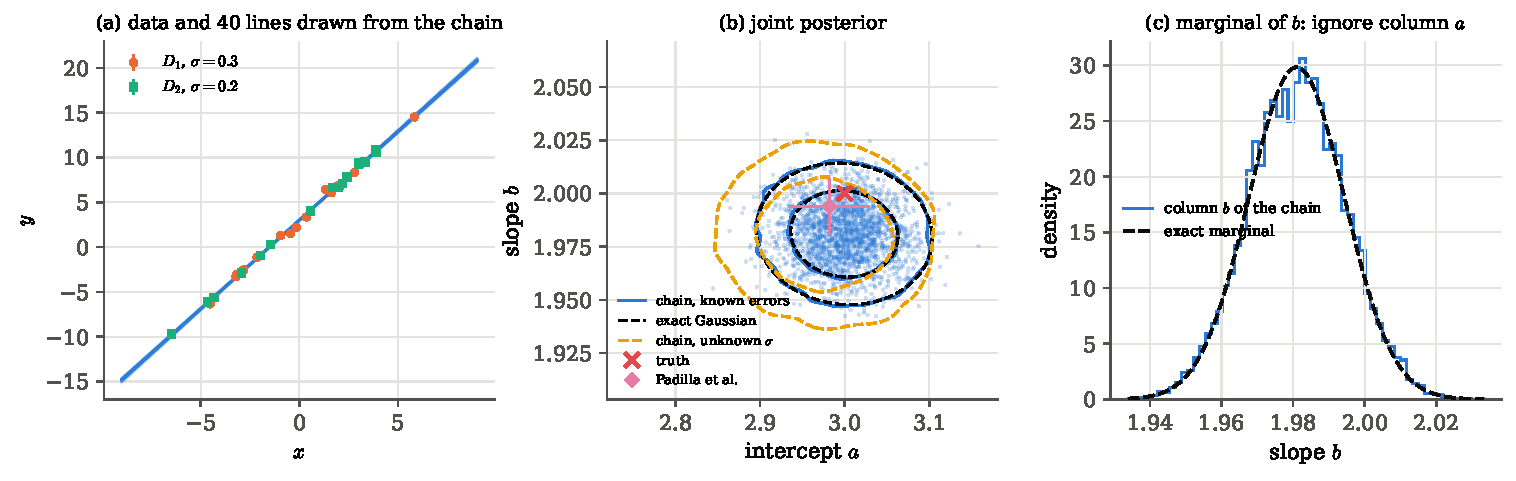
\includegraphics[width=\linewidth]{figures/ch09/line_fit.pdf}
\caption{The straight line. (a) The two data sets and 40 lines whose $(a,b)$ were picked at random
from the chain; they all pass through the bulk of the points. (b) The joint posterior: chain samples
(dots) with their 68 and 95 per cent contours (solid), the exact Gaussian (black dashed), the
posterior when the noise level is an unknown parameter (orange dashed), the truth (cross) and the
result of Padilla et al.\ (diamond with error bars). (c) The histogram of the $b$ column of the
chain against the exact marginal density of $b$.}
\label{9c:fig:line-fit}
\end{figure}

\subsection{Marginalising by ignoring a column}
\label{9c:sec:line-marginal}

The chain is a table with one row per step and one column per parameter. Suppose we care only
about the slope. Its marginal posterior is $p(b\given\data)=\int p(a,b\given\data)\,\dd a$: the
joint density with the nuisance parameter $a$ averaged out, exactly the operation that
\cref{ch:01} introduced to isolate one variable of a joint distribution. With a chain we never do
that integral. We take the $b$ column, throw the $a$ column away, and histogram what is left
(\cref{9c:fig:line-fit}c, \cref{9c:fig:column}).

\begin{keyidea}[A column of the chain is a sample of the marginal]
If the rows $(a_t,b_t)$ are draws from $p(a,b\given\data)$, the numbers $b_t$ alone are draws from
$p(b\given\data)$. Marginalising over any nuisance parameter costs nothing: drop its column.
\end{keyidea}

Why is this true? Take any interval $B$ of slopes and ask how often a row of the chain has its
slope in $B$, whatever its intercept:
\begin{align}
  \Prob(b_t\in B)
  &\eqby{1}\int\!\!\int \mathbb 1_B(b)\,p(a,b\given\data)\,\dd a\,\dd b
   \eqby{2}\int_B\Bigl[\int p(a,b\given\data)\,\dd a\Bigr]\dd b
   \eqby{3}\int_Bp(b\given\data)\,\dd b .
  \label{9c:eq:column}
\end{align}
\begin{explain}
  \item The row $(a_t,b_t)$ is distributed as the joint posterior, and the event ``$b_t\in B$''
        puts no condition on $a_t$: its indicator $\mathbb 1_B(b)$ is one for every $a$ when $b\in B$.
  \item The indicator restricts the $b$ integral to $B$; the $a$ integral is done first.
  \item The inner integral is the marginal density, by definition.
\end{explain}
A histogram counts rows with $b_t$ in each bin, so by \eqref{9c:eq:column} and the ergodic theorem
(\cref{9a:sec:ergodic}) it converges to the marginal. The column does the integral for us because
the rows with large $|a-\hat a|$ already appear less often, in proportion to their posterior weight.
The same holds in any dimension: from a chain in 6 or 30 parameters, every one- and
two-dimensional marginal is a histogram of one or two columns. This is how the marginals of
\cref{9c:fig:line-fit}, and all the triangle plots that follow, are made
\srcref{HobsonBMC}{p.~71}.

\begin{figure}[htbp]
\centering
\begin{tikzpicture}[font=\small]
  \node[anchor=south west] at (0,3.05) {chain};
  \draw[black!50] (0,0) rectangle (2.6,3.0);
  \draw[black!50] (1.3,0) -- (1.3,3.0);
  \node at (0.65,2.75) {$a_t$};
  \node at (1.95,2.75) {$b_t$};
  \draw[black!30] (0,2.5) -- (2.6,2.5);
  \foreach \y/\a/\b in {2.2/2.98/1.97,1.8/3.03/1.99,1.4/3.03/1.99,1.0/2.95/1.98,0.6/3.01/2.00,0.25/{\vdots}/{\vdots}}{
    \node[black!45] at (0.65,\y) {\a};
    \node[formblue] at (1.95,\y) {\b};
  }
  \fill[black!8,opacity=0.6] (0,0) rectangle (1.3,2.5);
  \node[black!55,font=\footnotesize,align=center] at (0.65,-0.45) {dropped};
  \node[formblue,font=\footnotesize,align=center] at (1.95,-0.45) {kept};
  \draw[->,thick,black!60] (3.0,1.5) -- (4.3,1.5);
  \begin{scope}[xshift=4.8cm]
    \draw[->,black!60] (0,0) -- (4.4,0) node[right] {$b$};
    \foreach \x/\h in {0.2/0.10,0.6/0.38,1.0/0.95,1.4/1.75,1.8/2.45,2.2/2.6,2.6/2.05,3.0/1.25,3.4/0.6,3.8/0.2}{
      \fill[formblue!35] (\x-0.2,0) rectangle (\x+0.2,\h);
      \draw[formblue!80!black,thin] (\x-0.2,0) rectangle (\x+0.2,\h);
    }
    \draw[thick,black,dashed,domain=0:4.0,samples=60] plot (\x,{2.62*exp(-((\x-2.1)^2)/(2*0.75^2))});
    \node[anchor=west,font=\footnotesize] at (2.9,2.7) {$p(b\given\data)$};
  \end{scope}
\end{tikzpicture}
\caption{Marginalising with a chain. Each row of the chain is a draw from the joint posterior.
Dropping the column of the nuisance parameter $a$ and histogramming the column $b$ gives the
marginal density of $b$ (dashed), with $a$ integrated out.}
\label{9c:fig:column}
\end{figure}

\paragraph{Example: marginal is not conditional.} It is tempting to report the width of $b$ ``at
the best $a$'', that is, the width of the slice $p(b\given a=\hat a,\data)$. Is that the same number?
\eqref{9c:eq:complete-square} answers it. Hold $a$ fixed in the quadratic form
$(\params-\hat\params)\T\Fish(\params-\hat\params)$; what is left is a quadratic in $b$ whose $b^2$
coefficient is $F_{bb}=S_{xx}$, and completing the square in $b$ once more turns it into
$S_{xx}(b-b_0)^2$ plus terms free of $b$. So the slice is a Gaussian of variance $1/S_{xx}$, whatever
the value at which $a$ was fixed. The marginal variance is the $bb$ element of $\Fish^{-1}$ in
\eqref{9c:eq:line-2x2}, $\sigma_b^2=S/\Delta$. To compare the two, multiply the marginal by $1-\rho^2$:
\begin{align}
  \sigma_b^2(1-\rho^2)
  &\eqby{1}\frac{S}{\Delta}\Bigl(1-\frac{S_x^2}{SS_{xx}}\Bigr)
   \eqby{2}\frac{S}{\Delta}\,\frac{SS_{xx}-S_x^2}{SS_{xx}}
   \eqby{3}\frac{1}{S_{xx}} .
  \label{9c:eq:slice}
\end{align}
\begin{explain}
  \item $\sigma_b^2=S/\Delta$ and $\rho^2=S_x^2/(SS_{xx})$, both from \eqref{9c:eq:line-2x2}.
  \item Common denominator.
  \item The numerator is $\Delta$ by its definition, and it cancels.
\end{explain}
So the slice has standard deviation $\sigma_b\sqrt{1-\rho^2}$, while the marginal has $\sigma_b$: fixing
$a$ forgets the uncertainty in $a$, which, through the correlation, would have spread $b$. With our data $\rho=\NineCLineRho$ and the two agree to a fraction of a per cent. With
the same data plotted against $x+\NineCLineShift$ (next subsection) the correlation becomes
$\rho=\NineCLineRhoShift$, so $1-\rho^2\approx0.088$ and the slice is $\sqrt{1-\rho^2}\approx0.30$ times
the marginal width:
reporting it would claim the slope three times better than the data know it. The column histogram
cannot make this mistake, because it never fixes $a$.

\paragraph{Example: the lines the posterior believes.} Each row of the chain is a whole line, so a
random selection of rows draws the family of lines compatible with the data
(\cref{9c:fig:line-fit}a; Kruschke calls these the credible regression lines
\srcref{Kruschke}{§17.2.4}). At a new $x$ the predicted mean $a+bx$ has variance
\[
  \Var(a+bx)=\sigma_a^2+2x\,\Cov(a,b)+x^2\sigma_b^2 ,
\]
smallest near the weighted centre of the data and growing quadratically away from it. With our
numbers the band is $\pm\NineCLineSa$ wide at $x=0$ and about
$\sqrt{0.042^2+10^2\times0.013^2}\approx0.14$ at $x=10$, outside the measured range: the lines fan
out where there are no data to pin them. The chain gives this without any error propagation:
compute $a_t+b_tx$ row by row and take the spread.

\subsection{Reproducing Padilla et al.: why their error bars are wider}
\label{9c:sec:line-padilla}

\paragraph{Their question.} Padilla et al.\ use this straight line as the first test of a sampler written for
cosmology \srcref{Padilla}{§5.1}. They wanted to know whether a short Metropolis run recovers the two
parameters of a line measured by two experiments, and what the error bars it reports mean. The first half of
the question has the answer ``yes'' in their paper and in ours. The second half is the interesting one,
because their error bars turn out to answer a different question from ours.

\paragraph{Their setup, one item at a time.} \emph{The data:} two sets of 16 points from the line $y=3+2x$, at
$x$ values drawn as $3\times\Normal(0,1)$, one set with Gaussian errors of $0.3$ and one with $0.2$. This is
our experiment exactly, but a different random realisation of it. \emph{The prior:} flat in the box $0<a<5$,
$0<b<3$, as ours. \emph{The noise:} here the two analyses part. The paper's text gives the two error bars,
but the analysis notebook in the repository the paper cites does not use them. It describes the noise of all
32 points by one common standard deviation $\sigma$, which it treats as unknown, with a flat prior on
$0<\sigma<1.5$. So $\sigma$ is a third parameter: the chain samples $(a,b,\sigma)$, and the numbers reported
for $a$ and $b$ come from the first two columns.

\paragraph{Their key equation: the line with the noise level integrated out.} In our notation the
change is one substitution. Set every $\sigma_i$ of \eqref{9c:eq:line-like} equal to the one unknown
$\sigma$. The exponent becomes $-\mathrm{RSS}(a,b)/2\sigma^2$, with the \newterm{residual sum of squares}
$\mathrm{RSS}=\sum_i(y_i-a-bx_i)^2$ \unpack{the $\chi^2$ of the line with all errors set to one}, and the
prefactor $\prod_i(\sqrt{2\pi}\,\sigma_i)^{-1}$ becomes $(2\pi)^{-N/2}\sigma^{-N}$. That prefactor could be
dropped when the $\sigma_i$ were known; now it depends on a parameter and must stay. With the flat priors,
$\ln p(a,b,\sigma\given\data)=-N\ln\sigma-\mathrm{RSS}(a,b)/2\sigma^2+\text{const}$. The noise level is a
nuisance parameter, and integrating it out (the upper prior limit is far out in the tail and can be sent to
infinity) gives
\begin{align}
  p(a,b\given\data)
  &\eqby{1}\int_0^\infty\sigma^{-N}e^{-\mathrm{RSS}/2\sigma^2}\,\dd\sigma
   \eqby{2}\frac12\Bigl(\frac{2}{\mathrm{RSS}}\Bigr)^{(N-1)/2}\int_0^\infty u^{(N-3)/2}e^{-u}\,\dd u
   \nonumber\\
  &\eqby{3}\frac12\,\Gamma\Bigl(\frac{N-1}{2}\Bigr)\Bigl(\frac{2}{\mathrm{RSS}}\Bigr)^{(N-1)/2}
   \;\propto\;\mathrm{RSS}(a,b)^{-(N-1)/2}
   \nonumber\\
  &\eqby{4}\Bigl[1+\frac{(\params-\hat\params_0)\T\mathbf A\T\mathbf A(\params-\hat\params_0)}{\mathrm{RSS}_{\min}}\Bigr]^{-(\nu+2)/2},
  \qquad \nu=N-3 .
  \label{9c:eq:line-student}
\end{align}
\begin{explain}
  \item Flat prior in $\sigma$; dropped constants. Marginalising $\sigma$ is integrating it out.
  \item Substitute $u=\mathrm{RSS}/2\sigma^2$: $\sigma=(\mathrm{RSS}/2u)^{1/2}$,
        $\dd\sigma=-\tfrac12(\mathrm{RSS}/2)^{1/2}u^{-3/2}\dd u$, and
        $\sigma^{-N}=(2u/\mathrm{RSS})^{N/2}$; the powers of $u$ combine to $u^{(N-3)/2}$, and the minus
        sign is absorbed by swapping the limits.
  \item $\int_0^\infty u^{s-1}e^{-u}\dd u=\Gamma(s)$ with $s=(N-1)/2$.
  \item \eqref{9c:eq:complete-square} with $\mathbf W=\Id$:
        $\mathrm{RSS}=\mathrm{RSS}_{\min}+(\params-\hat\params_0)\T\mathbf A\T\mathbf A(\params-\hat\params_0)$, $\hat\params_0$
        the ordinary least-squares line; divide by $\mathrm{RSS}_{\min}$ and write
        $(N-1)/2=(\nu+2)/2$.
\end{explain}
The last line is a two-dimensional Student $t$ density with $\nu=\NineCLineSnu$ degrees of freedom
(\cref{ch:02}), centred on the ordinary least-squares line, with covariance
$\mathrm{RSS}_{\min}(\mathbf A\T\mathbf A)^{-1}/(\nu-2)$. Set it beside the known-error posterior of
\cref{9c:sec:line-exact}. There the covariance was $(\mathbf A\T\mathbf W\mathbf A)^{-1}$, which for one
known noise level $\sigma$ ($\mathbf W=\Id/\sigma^2$) is $\sigma^2(\mathbf A\T\mathbf A)^{-1}$. The symbol map is
therefore short: their $\sigma^2$ is not given but estimated, and in the covariance it is replaced by
$\mathrm{RSS}_{\min}/(\nu-2)$, the scatter the data actually show about the best line; the Gaussian becomes a
Student $t$, with heavier tails, because that estimate is itself uncertain. The widths now depend on the data
through $\mathrm{RSS}_{\min}$. The common $\sigma$ must absorb the larger scatter of $D_1$, and the data put it at
$\sqrt{\mathrm{RSS}_{\min}/(N-2)}=\NineCLineSrms$, above the $0.2$ of the better experiment.

\paragraph{What we compute.} Two posteriors for our realisation: the known-error one of
\cref{9c:sec:line-chain}, and the unknown-$\sigma$ one, sampled by a chain in $(a,b,\sigma)$ whose $\sigma$ column
is then ignored (\cref{9c:sec:line-marginal}) and checked against the exact Student $t$ of
\eqref{9c:eq:line-student}. The chain gives $a=\NineCLineSAmc\pm\NineCLineSSamc$,
$b=\NineCLineSBmc\pm\NineCLineSSbmc$ (acceptance $\NineCLineSAcc$, largest $\hat R=\NineCLineSRmax$), against
the exact $\NineCLineSAex\pm\NineCLineSSaex$ and $\NineCLineSBex\pm\NineCLineSSbex$; the data say
$\sigma=\NineCLineSSigmc\pm\NineCLineSSSigmc$. Because their realisation differs from ours, one data set
cannot settle which model they used, so we also simulate $\NineCLineNrep$ replications of the whole design,
new $x_i$ and new $y_i$ each time, and record the widths each model would report.

\paragraph{Side by side.} Padilla et al.\ report $a=2.982\pm0.047$ and $b=1.994\pm0.013$
\srcref{Padilla}{§5.1}.
\begin{center}
\small
\renewcommand{\arraystretch}{1.15}
\begin{tabular}{@{}lccc@{}}
\toprule
 & $a$ & $b$ & noise model\\\midrule
Padilla et al.\ \srcref{Padilla}{§5.1} & $2.982\pm0.047$ & $1.994\pm0.013$ & as published\\
ours, chain, known $\sigma_i$ & $\NineCLineAmc\pm\NineCLineSamc$ & $\NineCLineBmc\pm\NineCLineSbmc$ & $0.3$ and $0.2$ known\\
ours, exact, known $\sigma_i$ & $\NineCLineAhat\pm\NineCLineSa$ & $\NineCLineBhat\pm\NineCLineSb$ & \eqref{9c:eq:complete-square}\\
ours, chain, one unknown $\sigma$ & $\NineCLineSAmc\pm\NineCLineSSamc$ & $\NineCLineSBmc\pm\NineCLineSSbmc$ & $\sigma$ column ignored\\
ours, exact, one unknown $\sigma$ & $\NineCLineSAex\pm\NineCLineSSaex$ & $\NineCLineSBex\pm\NineCLineSSbex$ & Student $t$ \eqref{9c:eq:line-student}\\
typical width, unknown $\sigma$ & $\NineCLineSSaLo$--$\NineCLineSSaHi$ & $\NineCLineSSbLo$--$\NineCLineSSbHi$ & $\NineCLineNrep$ replications\\
\bottomrule
\end{tabular}
\end{center}

\paragraph{Why they differ.} \emph{The centres.} Their data are a different random realisation of the same
experiment, so their centres must differ from ours by amounts of order one standard deviation, and they do.

\emph{The widths cannot come from the known errors.} With known errors the posterior covariance $\Fish^{-1}$
depends on the $x_i$ and $\sigma_i$ only, not on the $y_i$ \eqref{9c:eq:line-2x2}, and $\sigma_a$ can exceed
its floor $1/\sqrt S$ only through the factor $(1-\bar x_w^2/\overline{x^2}_w)^{-1/2}$. How large would that
factor have to be? Write $r^2=\bar x_w^2/\overline{x^2}_w$ for the squared ratio of the weighted mean of the
$x_i$ to their weighted root-mean-square. Then
\begin{align}
  \frac{0.047}{\NineCLineSaFloor}\approx1.13
  \quad&\eqby{1}\quad\frac{1}{1-r^2}=1.13^2\approx1.28
  \quad\eqby{2}\quad r^2\approx0.22,\qquad r\approx0.47 .
  \label{9c:eq:padilla-r}
\end{align}
\begin{explain}
  \item The floor is $1/\sqrt S$ with $S=16/0.3^2+16/0.2^2=578$, so $1/\sqrt S=\NineCLineSaFloor$; by
        \eqref{9c:eq:line-2x2} the ratio $\sigma_a\sqrt S$ is $(1-r^2)^{-1/2}$. Square it.
  \item Solve: $r^2=1-1/1.28$.
\end{explain}
So the weighted mean of the $x_i$ would have to be about half their root-mean-square. For 32 points drawn
from $3\times\Normal(0,1)$ the root-mean-square is about $3$, while the mean scatters about zero with standard
deviation about $3/\sqrt{32}\approx0.53$; a typical $r$ is therefore $0.53/3\approx0.18$, and $0.47$ is
more than two and a half times that. The replications confirm it: the known-error width $\sigma_a$ has
median $\NineCLineKSaMed$ with 68 per cent between $\NineCLineKSaLo$ and $\NineCLineKSaHi$, and
$\NineCLineKPadSaPct$ per cent of replications give less than Padilla's $0.047$. Their posterior is not
the posterior of \eqref{9c:eq:line-logpost}.

\emph{The widths do come from one unknown $\sigma$.} Over the same $\NineCLineNrep$ replications the
unknown-$\sigma$ model gives $\sigma_a$ between $\NineCLineSSaLo$ and $\NineCLineSSaHi$ (68 per cent) and
$\sigma_b$ between $\NineCLineSSbLo$ and $\NineCLineSSbHi$; Padilla's widths sit at the
$\NineCLineSPadSaPct$th and $\NineCLineSPadSbPct$th percentiles, perfectly ordinary.\footnote{The paper also
says the chains were run ``with temperature $T=2$''. Read literally, a tempered chain samples $\Like^{1/2}$
and would widen the known-error posterior by $\sqrt2$, to about $0.059$ and $0.019$; neither those numbers
nor the known-error ones match the published widths, while the unknown-$\sigma$ model does.}

\paragraph{The lesson.} It is not about this paper. Two analyses of the same kind of data can both be correct and
quote different error bars because they put different hypotheses in the likelihood: ``the errors
are $0.3$ and $0.2$'' is a stronger statement than ``there is some common noise level'', and the
stronger statement buys tighter constraints. When reproducing a published number, find the model
first.

\subsection{Centring the predictor: the same posterior, a different chain}
\label{9c:sec:line-centre}

Kruschke points out that a regression chain can become very slow for a reason that has nothing to
do with the physics: the arbitrary position of $x=0$ \srcref{Kruschke}{§17.2.1.1}. Move the origin
of $x$ far from the data, and every line that goes through the data has to trade its slope against
its intercept, because tilting a line about the data cloud moves its value at the distant
$x=0$ by a lot. Equation \eqref{9c:eq:line-2x2} puts a number on it. With $x$ shifted by $s$, the
weighted means become $\bar x_w=s$ and $\overline{x^2}_w=s^2+v$, where $v=\NineCLineXrms^2$ is the
variance of our $x$ values, so
\[
  \rho_{ab}=-\frac{s}{\sqrt{s^2+v}}=-\frac{10}{\sqrt{100+\NineCLineXrms^2}}\approx-0.96
  \quad\text{for } s=10,
\]
and the intercept width grows from $\NineCLineSaCent$ to $\NineCLineSaShift$. The simulation, with
the same data plotted against $x-\bar x+\NineCLineShift$, gives $\rho=\NineCLineRhoShift$.

The posterior is the same physical statement in both coordinates: the intercept at the new origin
is the old one minus $s$ times the slope, a linear change of variables
\srcref{Kruschke}{eq.~17.2}. The chain is not the same. Run both with the same round proposal, of
radius equal to the centred intercept width: the centred chain accepts $\NineCLineAccCent$ of its
moves and has $\tau=\NineCLineTauCent$ steps; the shifted one accepts $\NineCLineAccShift$ and has
$\tau=\NineCLineTauShift$ steps, a factor of about 60 in run time for the same precision
(\cref{9c:fig:line-centring}). This is the narrow-diagonal problem of \cref{9b:sec:shaped}: a round
proposal on a thin tilted ellipse must take steps of the ellipse's short width and then diffuses
slowly along its length. There are two cures, and both are standard. Reparametrise so that the
posterior is round (centre or standardise $x$, as Kruschke does, then transform back with eq.~17.2),
or keep the parameters and give the proposal the shape of the posterior covariance, which is what
CosmoMC does with the covariance of a previous run \cite{LewisBridle2002}.

\begin{figure}[htbp]
\centering
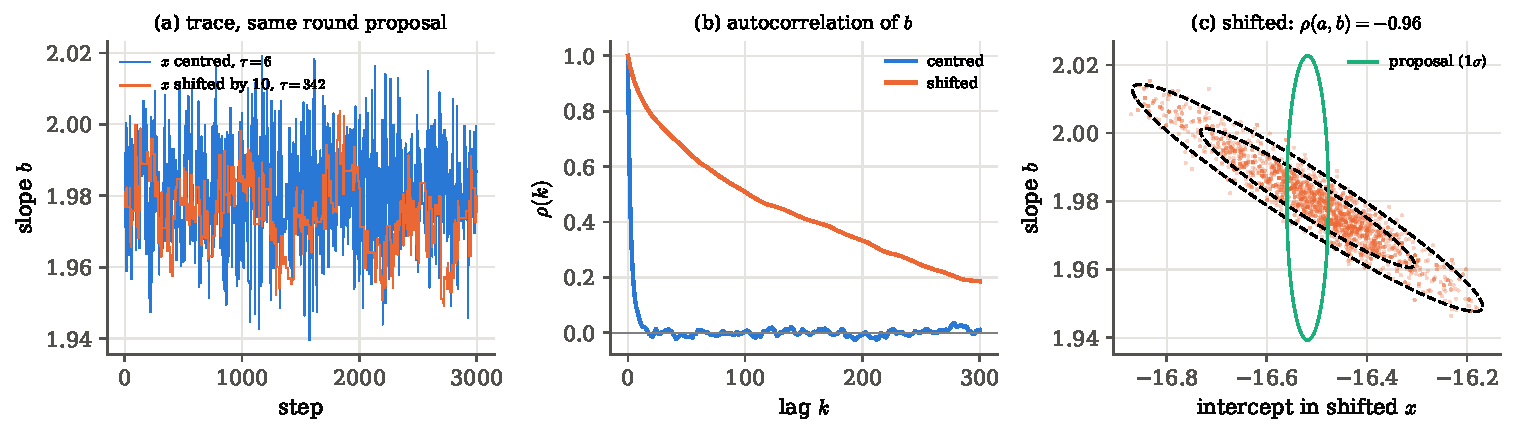
\includegraphics[width=\linewidth]{figures/ch09/line_centring.pdf}
\caption{The same straight-line posterior sampled with the same round proposal in two coordinate
systems. (a) Traces of the slope: with $x$ centred the chain jumps freely; with the origin of $x$
moved ten units from the data it creeps. (b) Their autocorrelation functions. (c) In shifted
coordinates the posterior (ellipse, 68 and 95 per cent) is a thin diagonal ridge, and the proposal
(green circle, one standard deviation) can only take steps of its short width.}
\label{9c:fig:line-centring}
\end{figure}
\section{A decaying source: curved posteriors and nuisance parameters}
\label{9c:sec:exp}

The straight line had a Gaussian posterior because the model was linear in its parameters. Most
physical models are not. A radioactive source, a cooling body, a charging capacitor, the light curve
of a supernova: each is an exponential in time, and the decay time enters inside the exponential.
For such models the posterior has no closed form, a Gaussian fitted at the peak is only an
approximation, and the chain becomes the instrument rather than a check. The same models also
bring the most common nuisance parameter of all, an unknown noise level.

\paragraph{The data.} A source is read once an hour for fifteen hours. The count rate falls as
$y(t)=Ae^{-t/\tau}$, and each reading has a Gaussian error of standard deviation $\sigma$. We
simulate $N=\NineCExpN$ readings at $t=0,1,\dots,14$\,h with $A=\NineCExpAtrue$\,s$^{-1}$,
$\tau=\NineCExpTautrue$\,h and $\sigma=\NineCExpSigtrue$\,s$^{-1}$ (\cref{9c:fig:exp-fit}a). The prior is
flat in $0<A<300$\,s$^{-1}$ and $0.1<\tau<30$\,h. With $\sigma$ known, the derivation of
\eqref{9c:eq:line-like} goes through unchanged with $a+bx_i$ replaced by $Ae^{-t_i/\tau}$:
\begin{equation}
  \ln p(A,\tau\given\data)=-\frac{\chi_0^2(A,\tau)}{2\sigma^2}+\text{const},
  \qquad
  \chi_0^2(A,\tau)=\sum_{i=1}^N\bigl(y_i-Ae^{-t_i/\tau}\bigr)^2 ,
  \label{9c:eq:exp-logpost}
\end{equation}
where $\chi^2_0$ is the residual sum of squares, not yet divided by $\sigma^2$.

\subsection{How far from Gaussian? The Laplace approximation and the chain}
\label{9c:sec:exp-laplace}

\paragraph{The question.} Is a Gaussian centred at the best fit a good description of this
posterior, and if not, does the chain notice? The Gaussian in question is the
\newterm{Laplace approximation} \unpack{the Gaussian whose log matches $\ln p$ to second order at
its peak}. It comes from a Taylor series of $\ln p$ about the maximum $\hat\params$:
\begin{align}
  \ln p(\params)
  &\eqby{1}\ln p(\hat\params)+(\params-\hat\params)\T\nabla\ln p\big|_{\hat\params}
     +\tfrac12(\params-\hat\params)\T\bigl[\nabla\nabla\T\ln p\bigr]_{\hat\params}(\params-\hat\params)+\dots
  \nonumber\\
  &\eqby{2}\ln p(\hat\params)-\tfrac12(\params-\hat\params)\T\mathbf H(\params-\hat\params)+\dots,
  \qquad H_{ij}=-\frac{\partial^2\ln p}{\partial\theta_i\partial\theta_j}\Big|_{\hat\params}.
  \label{9c:eq:laplace}
\end{align}
\begin{explain}
  \item Taylor's theorem in two variables.
  \item At a maximum the gradient vanishes. Defining $\mathbf H$ with a minus sign makes it positive
        definite there.
\end{explain}
Dropping the dots leaves a Gaussian with mean $\hat\params$ and covariance $\mathbf H^{-1}$, the same
object as $\Fish^{-1}$ in \eqref{9c:eq:complete-square}. For the line the dots were exactly zero. Here
we find the peak with a simplex optimiser and $\mathbf H$ by finite differences: $A=\NineCExpAhat\pm\NineCExpSaLap$,
$\tau=\NineCExpTauhat\pm\NineCExpStLap$\,h, $\rho=\NineCExpRhoLap$. Four chains of $\NineCExpNsteps$ steps,
with the Laplace covariance as the proposal shape, give $A=\NineCExpAMeanMC\pm\NineCExpASdMC$,
$\tau=\NineCExpTauMeanMC\pm\NineCExpTauSdMC$\,h, $\rho=\NineCExpRhoMC$ (acceptance $\NineCExpAccK$). The
widths agree with Laplace. The centre of $\tau$ does not: the posterior mean is above the peak. On a
$400\times400$ grid, where the exact posterior can be normalised and its $A$ direction summed out,
the marginal of $\tau$ has mean $\NineCExpTauMean$\,h, standard deviation $\NineCExpTauSd$\,h and
skewness $\NineCExpTauSkew$; the chain's column of $\tau$ has skewness $\NineCExpTauSkewMC$
(\cref{9c:fig:exp-fit}c). The joint contours are bent, a banana in miniature
(\cref{9c:fig:exp-fit}b).

\paragraph{Example: why the tail is on the long-$\tau$ side.} At the time $t=4$\,h the model
predicts $100e^{-1}=36.8$\,s$^{-1}$ for $\tau=4$\,h. Lower $\tau$ by one hour and the prediction falls
to $100e^{-4/3}=26.4$, a change of $10.4$; raise it by one hour and it rises to $100e^{-4/5}=44.9$, a
change of only $8.1$. The data resist a shorter decay time more strongly than a longer one, so the
likelihood falls faster on the short side and leaves a longer tail on the long side. The reason is
that $\tau$ enters as $1/\tau$ in the exponent, and $1/\tau$ compresses large values. A different
parameter choice, the decay rate $\lambda=1/\tau$, would give a more symmetric posterior, but then a
flat prior in $\lambda$ is a different prior from a flat prior in $\tau$ (the Jacobian
$|\dd\tau/\dd\lambda|=1/\lambda^2$ of \cref{ch:02}), and the question ``which is flat?'' must be
answered with the physics, not with convenience.

\begin{figure}[htbp]
\centering
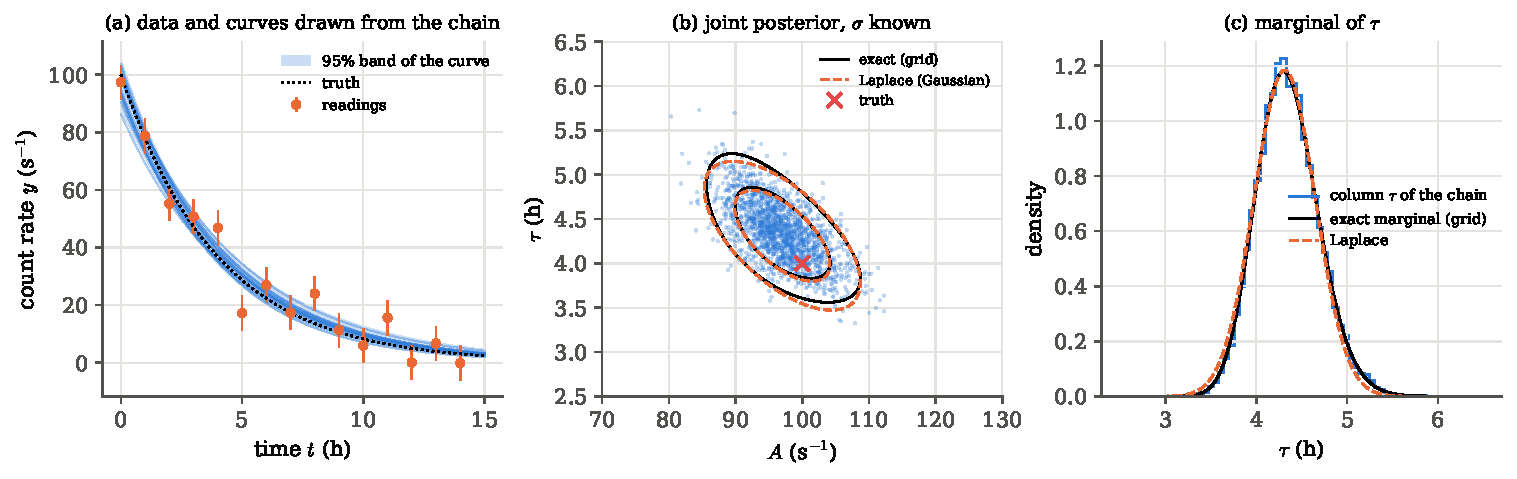
\includegraphics[width=\linewidth]{figures/ch09/exp_fit.pdf}
\caption{The decaying source with known noise. (a) The fifteen readings, the true curve (dotted),
fifteen curves whose $(A,\tau)$ were drawn from the chain, and the band containing 95 per cent of the
drawn curves at each time. (b) The joint posterior: chain samples, the exact contours computed on a
grid (black), and the Laplace ellipses (dashed), which miss the bend. (c) The marginal of $\tau$: the
chain's column, the exact marginal and the Laplace Gaussian, which puts the centre too low and misses
the tail at large $\tau$.}
\label{9c:fig:exp-fit}
\end{figure}

\subsection{The unknown noise level: three ways to treat a nuisance}
\label{9c:sec:exp-sigma}

So far $\sigma$ was given. In a real measurement it is often known only roughly, and it matters:
by \eqref{9c:eq:exp-logpost} every posterior width is proportional to it. There are three things one
can do with it.

\emph{Fix it at a guess.} If the guess is wrong, every width is wrong by the same factor. With
$\sigma=\NineCExpSigWrong$ instead of $\NineCExpSigtrue$, the marginal of $\tau$ has standard deviation
$\NineCExpTauSdWrong$\,h instead of $\NineCExpTauSd$, and nothing in the output signals the problem
(\cref{9c:fig:exp-sigma}a, dashed).

\emph{Integrate it out analytically.} Hobson et al.\ do this for a model with the same structure
\srcref{HobsonBMC}{eqs.~2.25--2.26}. With the prior $p(\sigma)\propto1/\sigma$ (flat in $\ln\sigma$,
the Jeffreys prior for a scale, \cref{ch:05}),
\begin{align}
  p(A,\tau\given\data)
  &\eqby{1}\int_0^\infty(2\pi\sigma^2)^{-N/2}e^{-\chi^2_0/2\sigma^2}\,\frac{\dd\sigma}{\sigma}
   \eqby{2}(2\pi)^{-N/2}\,\frac12\Bigl(\frac{2}{\chi^2_0}\Bigr)^{N/2}\int_0^\infty u^{N/2-1}e^{-u}\,\dd u
   \nonumber\\
  &\eqby{3}\frac{\Gamma(N/2)}{2\,\pi^{N/2}}\,\bigl[\chi^2_0(A,\tau)\bigr]^{-N/2}.
  \label{9c:eq:sigma-marg}
\end{align}
\begin{explain}
  \item The likelihood \eqref{9c:eq:exp-logpost} with its normalisation $(2\pi\sigma^2)^{-N/2}$ restored,
        because it depends on $\sigma$, times the prior $1/\sigma$ (its normalisation over a finite range
        of $\sigma$ is a constant and is dropped).
  \item The substitution $u=\chi_0^2/2\sigma^2$ of \eqref{9c:eq:line-student}, now with one more power
        of $1/\sigma$ from the prior: $\sigma^{-N-1}\dd\sigma=\tfrac12(2/\chi_0^2)^{N/2}u^{N/2-1}\dd u$.
  \item The Gamma integral with $s=N/2$; $(2\pi)^{-N/2}2^{N/2}=\pi^{-N/2}$.
\end{explain}
The shape $[\chi^2_0]^{-N/2}$ is exactly Hobson's eq.~(2.26); their prefactor is the large-$N$ form of
ours, from Stirling's formula for $\Gamma(N/2)$. Compare with the line: a flat prior on $\sigma$ gave the
power $-(N-1)/2$ in \eqref{9c:eq:line-student}, the scale prior $1/\sigma$ gives $-N/2$. Either way the
unknown noise turns $e^{-\chi^2/2}$ into a power law in $\chi^2$, which has heavier tails: the data
must now also estimate their own scatter, and every parameter is a little less certain. On the grid
the marginal of $\tau$ from \eqref{9c:eq:sigma-marg} has mean $\NineCExpTauMeanMarg$\,h and standard
deviation $\NineCExpTauSdMarg$\,h, wider than the $\NineCExpTauSd$\,h of the known-noise case.

\emph{Sample it and ignore its column.} Add $\ln\sigma$ to the chain as a third parameter with a flat
prior (the same $1/\sigma$ prior, written in the variable in which it is flat) and run:
\pyfile[firstline=58,lastline=74]{code/ch09/41_exponential.py}{Three parameters, or $\sigma$ integrated out}
The function \pyname{lp_three} is $-N\ln\sigma-\chi^2_0/2\sigma^2$ in the variable $\ln\sigma$, and
\pyname{lp_marg} is \eqref{9c:eq:sigma-marg}. By the key idea of \cref{9c:sec:line-marginal}, the $\tau$
column of the three-parameter chain is a sample of $p(\tau\given\data)$ with $\sigma$ integrated out, so
it must agree with the grid built on \eqref{9c:eq:sigma-marg}. It does: mean $\NineCExpTauMeanChain$\,h,
standard deviation $\NineCExpTauSdChain$\,h (four chains, acceptance $\NineCExpAccThree$, largest
$\hat R=\NineCExpRmax$; \cref{9c:fig:exp-sigma}a). The analytic integral and the ignored column are two
routes to the same marginal; the second needs no algebra and works for any prior.

The column we ignored is not useless either: it is the posterior of the noise level
(\cref{9c:fig:exp-sigma}b), $\sigma=\NineCExpSigMed$ with 68 per cent between $\NineCExpSigLo$ and
$\NineCExpSigHi$\,s$^{-1}$. That is the honest statement of how well fifteen readings determine their
own scatter, and its width is the reason the marginal of $\tau$ widened. Hobson et al.\ use the same
device for error bars that may be too small, scaling every $\sigma_i$ by one unknown factor and
marginalising it \srcref{HobsonBMC}{p.~52}; Padilla's notebook did exactly that for the straight
line of \cref{9c:sec:line-padilla}.

\begin{figure}[htbp]
\centering
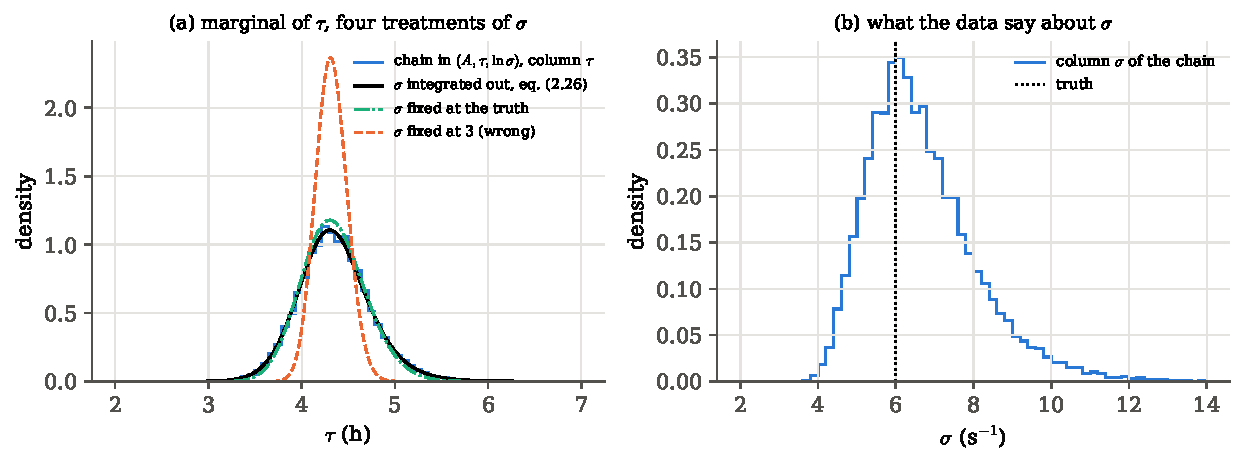
\includegraphics[width=0.92\linewidth]{figures/ch09/exp_sigma.pdf}
\caption{The noise level as a nuisance parameter. (a) The marginal of $\tau$ four ways: the $\tau$
column of the chain in $(A,\tau,\ln\sigma)$, which overlays the analytic marginal
\eqref{9c:eq:sigma-marg}; $\sigma$ fixed at its true value (narrower, since the uncertainty in $\sigma$ is
ignored); and $\sigma$ fixed at a wrong value, half the truth (far too narrow). (b) The $\sigma$ column of
the same chain: what the data say about their own scatter.}
\label{9c:fig:exp-sigma}
\end{figure}

\begin{pitfall}[A fixed nuisance parameter is a hidden assumption]
Fixing a nuisance parameter is marginalising it with a delta-function prior
\srcref{HobsonBMC}{p.~42}. It is legitimate when the parameter really is known; when it is not,
every width inherits the error of the guess, and the chain cannot tell. Before quoting a constraint,
list what was held fixed. \Cref{9c:sec:planck} will show that the error bar on $\ln(10^{10}A_s)$ from a
CMB temperature spectrum changes by a factor of nine depending on whether one parameter is fixed.
\end{pitfall}

\subsection{Data sets that disagree: hyperparameters}
\label{9c:sec:hyper}

Two laboratories measure the same quantity, each quotes an error bar, and the two results do not overlap.
One of them has underestimated its errors, or both have, and nobody knows which. Averaging them with their
stated weights gives a number with a small error bar that may be far from the truth; throwing one away by
judgement is arbitrary. Padilla et al.\ pose this for the straight line \srcref{Padilla}{§§3.10, 5.2}.

\paragraph{The question.} When two data sets disagree and we do not know which is wrong, can the analysis
itself discover that one does not belong and down-weight it, and can the data tell us whether doing so was
justified?

\paragraph{The setup.} Two cases, each with 16 points per data set and $x$ drawn as $3\times\Normal(0,1)$ as
before:
\begin{center}
\small
\renewcommand{\arraystretch}{1.15}
\begin{tabular}{@{}lll@{}}
\toprule
 & data set $D_1$ & data set $D_2$\\\midrule
case 1 (agree) & $y=3+2x$, $\sigma=0.3$ & $y=3+2x$, $\sigma=0.2$\\
case 2 (disagree) & $y=3+2x$, $\sigma=0.3$ & $y=3.5+1.5x$, $\sigma=0.5$\\
\bottomrule
\end{tabular}
\end{center}
Case 1 is the experiment of \cref{9c:sec:line}, in a new realisation. In case 2 the two sets come from different lines, but the analysis
is not told so. Two models of the data are compared.

\emph{$H_0$: both data sets as stated.} One line, and every point has the error bar its experiment quotes.
This is the likelihood \eqref{9c:eq:line-like} of the straight line applied to all 32 points. In case 2 the
single line lands between the two truths and fits neither; for our realisation
$a=\NineCHypAzero\pm\NineCHypSAzero$, $b=\NineCHypBzero\pm\NineCHypSBzero$, with a best-fit
$\chi^2\approx\NineCHypChiZero$ for 32 points (\cref{9c:fig:hyper}a, b). The posterior is confident and
wrong, because the likelihood was told that both data sets have the stated errors and describe the
same line.\footnote{Padilla et al.\ quote $a=3.528\pm0.056$, $b=1.795\pm0.014$ for their realisation.
By \eqref{9c:eq:line-2x2}, errors of $0.3$ and $0.5$ allow no intercept width below
$(16/0.3^2+16/0.5^2)^{-1/2}=0.064$ for any choice of the $x_i$, so the published widths were not
computed with these error bars; we do not try to reconstruct their setting.}

\emph{$H_1$: each data set may have its errors scaled by an unknown factor.} Still one line, but data set
$k$ gets a weight $\alpha_k$ that multiplies its $\chi^2_k$, which is the same as dividing its error bars by
$\sqrt{\alpha_k}$. With $\alpha_k=1$ the errors are as stated; a small $\alpha_k$ says ``these error bars are
underestimated''. The weights are unknown and are marginalised, one per data set: this is the
\newterm{hyperparameter method} \unpack{one extra weight per data set, unknown and integrated out}. We keep
Padilla's letters: $\alpha_k$ for the weight, $n_k$ for the number of points and $\chi^2_k$ for the
$\chi^2$ of data set $k$ alone, as in \eqref{9c:eq:line-like}; their covariance $\mathbf V$ of one data set is
our $\diag(\sigma_i^2)$.

\paragraph{The prior on a weight.} All we want to say about $\alpha$ is that it is positive and that the
stated errors are right on average, $\E\alpha=1$; nothing about how far a given experiment may stray. The
least committal density with that one property is the maximum-entropy density of \cref{2b:sec:maxent-recipe}
with a flat measure on $\alpha>0$. Maximise $-\int p\ln p\,\dd\alpha$ subject to $\int p\,\dd\alpha=1$ and
$\int\alpha\,p\,\dd\alpha=1$:
\begin{align}
  p(\alpha)
  &\eqby{1}\frac1Z\,e^{-\lambda\alpha}
   \eqby{2}\lambda\,e^{-\lambda\alpha}
   \eqby{3}e^{-\alpha},\qquad\alpha>0 .
  \label{9c:eq:alpha-prior}
\end{align}
\begin{explain}
  \item \eqref{2b:eq:maxent-solution} with one constraint, $f(\alpha)=\alpha$, and a flat measure; $\lambda$
        is its Lagrange multiplier.
  \item Normalisation: $Z=\int_0^\infty e^{-\lambda\alpha}\dd\alpha=1/\lambda$.
  \item The mean of $\lambda e^{-\lambda\alpha}$ is $1/\lambda$, and it must be one, so $\lambda=1$.
\end{explain}
A mean of one centres the weights on ``the errors are as quoted''; the exponential then lets an individual
weight be small (errors underestimated) without any further assumption.

\paragraph{Their key equation: the likelihood with the weight integrated out.} For one data set of $n$ points,
\begin{align}
  p(D_k\given\params,H_1)
  &\eqby{1}\int_0^\infty\frac{\alpha^{n/2}}{(2\pi)^{n/2}|\mathbf V|^{1/2}}\,e^{-\alpha\chi^2/2}\,e^{-\alpha}\,\dd\alpha
   \eqby{2}\frac{1}{(2\pi)^{n/2}|\mathbf V|^{1/2}}\,
     \frac{\Gamma(n/2+1)}{(\chi^2/2+1)^{n/2+1}}
   \nonumber\\
  &\eqby{3}\frac{2\,\Gamma(n/2+1)}{\pi^{n/2}|\mathbf V|^{1/2}}\,(\chi^2+2)^{-(n/2+1)} .
  \label{9c:eq:hyper}
\end{align}
\begin{explain}
  \item Errors $\sigma_i/\sqrt\alpha$: each of the $n$ Gaussian factors gains $\sqrt\alpha$ in its
        normalisation and $\alpha$ in its exponent. Times the prior \eqref{9c:eq:alpha-prior}.
  \item $\int_0^\infty\alpha^{s-1}e^{-c\alpha}\dd\alpha=\Gamma(s)/c^s$ with $s=n/2+1$ and $c=\chi^2/2+1$.
  \item $(\chi^2/2+1)^{-(n/2+1)}=2^{n/2+1}(\chi^2+2)^{-(n/2+1)}$, and $2^{n/2+1}/(2\pi)^{n/2}=2/\pi^{n/2}$.
\end{explain}
This is Padilla's eq.~(50), and the $H_1$ likelihood of the two data sets is the product of one such factor per
set. The Gaussian $e^{-\chi^2/2}$ has become the power law $(\chi^2+2)^{-(n/2+1)}$,
the same thing that happened to the unknown $\sigma$ in \eqref{9c:eq:sigma-marg}, now once per data set.
A power law is forgiving: a line that misses one data set badly is penalised only logarithmically in
that set's $\chi^2$, so the posterior can follow the other.

\paragraph{What the posterior does.} Under $H_1$ the posterior of $(a,b)$ has two peaks
(\cref{9c:fig:hyper}c): one at the line of $D_1$, carrying $\NineCHypWup$ of the probability, and one near
$(a,b)=(\NineCHypAlow,\NineCHypBlow)$, towards the line of $D_2$, whose peak is lower by a factor
$e^{\NineCHypDpeak}$ and carries a fraction $\NineCHypWlow$. The better data set wins, because its smaller
errors make it more informative. These weights come from integrating the posterior on a grid. Six
chains started at random in the prior box do not find them: none of the $\NineCHypChainsN$ chains
crossed between the peaks in 20\,000 steps, each spending more than 98 per cent of its steps in a single
peak. A chain started near the minor peak would stay there and report it as the whole posterior, and a
plot of the points of several chains shows the peaks with whatever density the starting points happened
to give them. This is the trap of
\cref{9b:sec:rhat} in practice. When the posterior is multimodal, histograms of chain points are not
evidence about the relative weights of the modes; a tempered or nested sampler, or a direct
integral as here, is needed.

\paragraph{Should we use $H_1$? The evidence ratio.} Adding hyperparameters is a choice of model, and
\cref{ch:05} answers such questions with the evidence $Z=\int\Like(\params)\,p(\params)\,\dd\params$ and the
Bayes factor $K=Z_1/Z_0$. Both models share the flat prior on $(a,b)$, here the box
$-5<a<8$, $0<b<4$, and both $Z$ are two-dimensional integrals, which we do by quadrature on a
$1301\times801$ grid. For the disagreeing data sets (case 2) we find $\ln K=\NineCHypLnKtwo$, a factor of
order $10^{17}$ in favour of $H_1$; for the agreeing ones (case 1), $K=\NineCHypKone$.

Where does a factor of $10^{17}$ come from? An integral over a likelihood with one sharp peak is the height
of the peak times its width, so $\ln K$ is the difference of the two log-likelihoods at their peaks plus a
difference of log-widths (the Occam terms of \cref{ch:05}), which are a few units at most. The heights carry
the effect. The normalisation $(2\pi)^{-n_k/2}|\mathbf V|^{-1/2}$ is common to the two models and cancels. With
$n_k=16$, so that $n_k/2+1=9$ and $\ln\Gamma(9)=\ln40\,320=10.6$, case 2 gives:
\begin{itemize}[itemsep=1pt]
  \item $H_0$ at its best line: $-\chi^2_{\min}/2=-\NineCHypChiZero/2=-79$. An acceptable fit of 32 points
        would have $\chi^2$ near 32 (the mean of a $\chi^2$ is its number of degrees of freedom), so the single
        line is worse than an acceptable fit by $e^{-(158-32)/2}=e^{-63}$.
  \item $H_1$ at its main peak, the line of $D_1$: by line~2 of \eqref{9c:eq:hyper} each set contributes
        $\ln\Gamma(9)-9\ln(\chi^2_k/2+1)$. $D_1$ fits its own line, $\chi^2_1\approx16$, giving
        $10.6-9\ln9=-9.2$. $D_2$ misses that line by $(3.5+1.5x)-(3+2x)=0.5(1-x)$, whose mean square over
        $x\sim3\times\Normal(0,1)$ is $0.25(1+9)=2.5$; adding the noise variance $0.25$ and dividing by $0.5^2$
        gives about $11$ per point, $\chi^2_2\approx176$, and a contribution $10.6-9\ln89=-29.8$. In all, $-39$.
\end{itemize}
The difference is $-39-(-79)=40$, against the quadrature's $\NineCHypLnKtwo$. The decisive item is the
treatment of $D_2$: under $H_0$ a misfit of $\chi^2_2\approx176$ costs $176/2=88$ in $\ln\Like$, under $H_1$ it
costs $9\ln89\approx40$ less a constant, because the power law charges the logarithm of $\chi^2$ rather than
$\chi^2$ itself. No Occam penalty from two extra parameters can compensate for that. The same count for case 1,
where both sets fit their common line with $\chi^2_k\approx16$ each, gives $H_1$ two terms of $-9.2$
against $H_0$'s $-32/2=-16$, a difference of about $-2$: the weights buy nothing when the errors are right
and cost a little. The power law's broader peak gives back part of that in the width term, and the quadrature
gives $\ln K=\NineCHypLnKone$, mildly in favour of $H_0$.

\paragraph{Side by side.} Padilla et al.\ quote Bayes factors for both cases.
\begin{center}
\small
\renewcommand{\arraystretch}{1.15}
\begin{tabular}{@{}lcc@{}}
\toprule
 & case 1 (data sets agree) & case 2 (data sets disagree)\\\midrule
Padilla et al., $K$ \srcref{Padilla}{eqs.~71--72} & $3$ & $37$\\
ours, $K=Z_1/Z_0$ by quadrature & $\NineCHypKone$ ($\ln K=\NineCHypLnKone$) & $\ln K=\NineCHypLnKtwo$\\
verdict \cite{KassRaftery1995} & barely worth a mention & decisive for $H_1$\\
\bottomrule
\end{tabular}
\end{center}

\paragraph{Why they differ.} The verdicts agree; the case-2 numbers differ by $\ln(4\times10^{17}/37)\approx37$
$e$-folds. The published values come from Padilla's eq.~(51), which is not an evidence ratio. To see what it
should have been as a ratio of likelihoods, divide \eqref{9c:eq:hyper} by the Gaussian likelihood of the same
data set at the same $\params$:
\begin{align}
  \frac{p(D_k\given\params,H_1)}{p(D_k\given\params,H_0)}
  &\eqby{1}\frac{2\,\Gamma(n/2+1)\,\pi^{-n/2}|\mathbf V|^{-1/2}(\chi^2+2)^{-(n/2+1)}}
              {(2\pi)^{-n/2}|\mathbf V|^{-1/2}e^{-\chi^2/2}}
   \nonumber\\
  &\eqby{2}2\,(2\pi)^{n/2}\pi^{-n/2}\;\Gamma(n/2+1)\,(\chi^2+2)^{-(n/2+1)}\,e^{+\chi^2/2}
   \nonumber\\
  &\eqby{3}2^{n/2+1}\,\Gamma(n/2+1)\,(\chi^2+2)^{-(n/2+1)}\,e^{+\chi^2/2}.
  \label{9c:eq:hyper-ratio}
\end{align}
\begin{explain}
  \item Numerator \eqref{9c:eq:hyper}; denominator the Gaussian likelihood \eqref{9c:eq:line-like} written with
        $\mathbf V=\diag(\sigma_i^2)$.
  \item $|\mathbf V|^{-1/2}$ cancels; dividing by $e^{-\chi^2/2}$ is multiplying by $e^{+\chi^2/2}$.
  \item $2\,(2\pi)^{n/2}/\pi^{n/2}=2\cdot2^{n/2}=2^{n/2+1}$.
\end{explain}
For two data sets the ratio is the product over $k$. Eq.~(51) as printed reads
$K=\prod_k2^{n_k/2+1}\Gamma(n_k/2+1)e^{-\chi^2_k/2}/(\chi^2_k+2)$. Three things separate it from $K=Z_1/Z_0$,
each sized here for case 2 at the $H_0$ best fit, where the two $\chi^2_k$ add up to $\NineCHypChiZero$:
\begin{enumerate}[itemsep=1pt]
  \item \emph{The power of $(\chi^2_k+2)$}: $1$ in print, $n_k/2+1=9$ in \eqref{9c:eq:hyper-ratio}. The missing
        factor $(\chi^2_k+2)^{-8}$ per set is $8\sum_k\ln(\chi^2_k+2)$ $e$-folds, between 46 and 70 however the
        158 is split between the two sets.
  \item \emph{The sign of $\chi^2_k/2$}: $e^{-\chi^2_k/2}$ in print, $e^{+\chi^2_k/2}$ in \eqref{9c:eq:hyper-ratio}.
        Together the two sets differ by $e^{\sum_k\chi^2_k}=e^{158}$.
  \item \emph{A ratio at one point is not a ratio of integrals.} Even corrected, \eqref{9c:eq:hyper-ratio}
        compares the two likelihoods at one $\params$, while $Z_1/Z_0$ integrates each over its own prior, and
        the two models peak at different lines. At the $H_0$ best fit the corrected ratio is
        $\sum_k[9\ln2+\ln\Gamma(9)-9\ln(\chi^2_k+2)]+79$, between 34 and 61 $e$-folds depending on the split,
        against $\ln K=\NineCHypLnKtwo$; at another $\params$ it would be another number.
\end{enumerate}
We cannot say which combination of these produced the published $37$, since the paper does not give the point
at which eq.~(51) was evaluated.

\paragraph{The lesson.} A Bayes factor is a ratio of integrals over the whole prior, and a likelihood ratio at
one point, however carefully written, is a different number, here by tens of $e$-folds. A direct integral (or, in
more dimensions, nested sampling or the importance-sampling identity of their eq.~48,
\cref{9c:sec:importance}) is the way to compute it.

\begin{figure}[htbp]
\centering
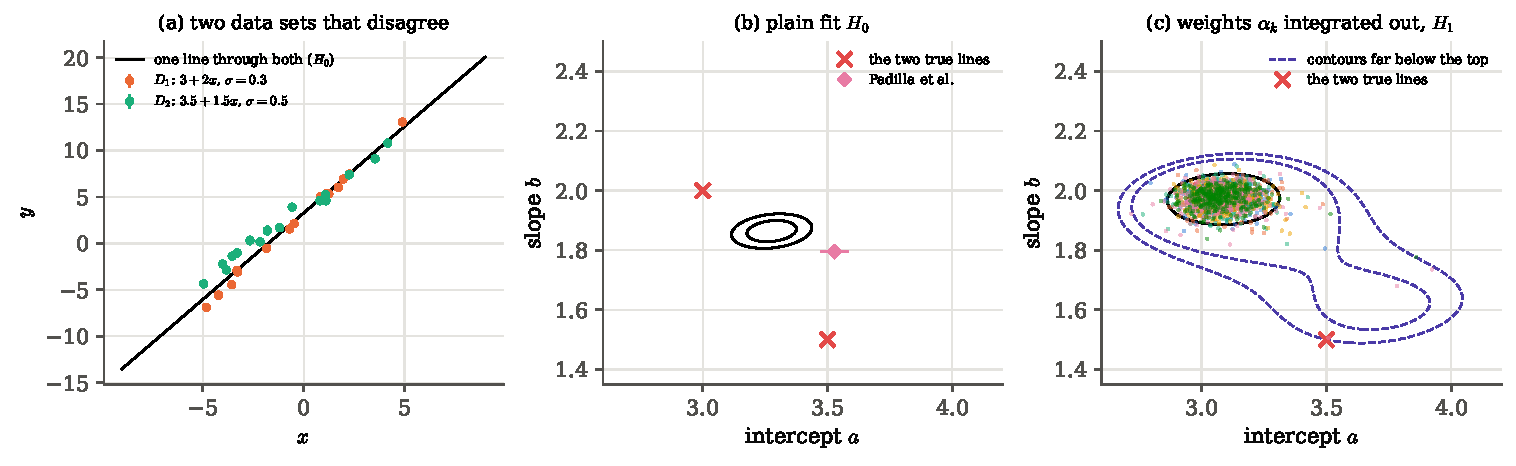
\includegraphics[width=\linewidth]{figures/ch09/hyper.pdf}
\caption{Two data sets drawn from different lines. (a) The data and the single line of $H_0$, which fits
neither. (b) The $H_0$ posterior (68 and 95 per cent), far from both true lines (crosses), with the
published result of Padilla et al.\ for their realisation. (c) With one marginalised weight per data
set ($H_1$): the posterior concentrates on the line of the more precise data set; contours drawn far
below the top (dashed) reveal the second, much lower peak towards the other line. Coloured points are
the six chains, each confined to a single peak.}
\label{9c:fig:hyper}
\end{figure}
\section{The likelihood of a CMB power spectrum}
\label{9c:sec:cl-like}

The straight line and the decaying source had data that were measurements of the model plus noise.
The CMB is different in kind. Cosmology does not predict the temperature in any direction of the
sky; it predicts the \emph{statistics} of the temperature field, its power spectrum $\Cell$, and the
sky we see is one random realisation of it (\cref{ch:07}). The data are therefore the
measured spectrum $\Chat$ of that one realisation, and the likelihood has to say how probable this
$\Chat$ is if the true spectrum were $\Cell$. On the full sky the answer is exact and short, and
every practical CMB likelihood is an approximation to it, so we derive it first and then test the
approximations against it.

\paragraph{The question in words.} It is the question of the straight line in
\cref{9c:sec:line}, asked in a much larger space of hypotheses. The observed event is the whole data
vector, here the measured spectrum $\Chat$ at every multipole at once, standing in for the map it was
computed from. The hypotheses are the cosmological models, one for every value of the $\Lambda$CDM
parameter vector, as the candidate lines were one for every pair $(a,b)$. To each hypothesis we put the
same question: if nature had chosen this model, how probable would it have been to observe exactly this
spectrum? That number, read as a function of the parameters, is the likelihood, and Bayes' theorem combines
it with the prior into a posterior over the models (\cref{5b:sec:continuous}). What is new for the CMB is
only the first step, the probability of a spectrum given a model.

\subsection{The chain of dependence: parameters, spectrum, sky}
\label{9c:sec:cl-hier}

Three levels connect the parameters to the data (\cref{9c:fig:hierarchy}). The parameters $\params$
(amplitude and tilt of the primordial spectrum, densities, optical depth) fix the angular power
spectrum through a Boltzmann code, $\Cell=\Cell(\params)$, with no randomness:
$\Cell=\sum_m\int\dd k\,T_m(\ell,k)P_m(k)$ in the notation of the cosmology notes, a weighted integral
of the primordial power over transfer functions (\cref{ch:T1} maps these objects). The spectrum fixes the \emph{distribution} of the
harmonic coefficients, $\alm\sim\Normal(0,\Cell)$, independent for different $\ell$ and $m$
(statistical isotropy, \cref{ch:07}). The coefficients give the map, and the map gives the data.
Hobson et al.\ write the posterior of the parameters with the middle level integrated out
\srcref{HobsonBMC}{eqs.~10.26--10.28}:
\begin{align}
  p(\params\given\data)
  &\eqby{1}\int\dd\Cell\;p(\params,\Cell\given\data)
   \eqby{2}\frac{1}{p(\data)}\int\dd\Cell\;p(\data\given\Cell)\,p(\Cell\given\params)\,p(\params)
   \nonumber\\
  &\eqby{3}\frac{p(\params)}{p(\data)}\int\dd\Cell\;p(\data\given\Cell)\,\delta\bigl(\Cell-\Cell(\params)\bigr)
   \eqby{4}\frac{p(\params)}{p(\data)}\,p\bigl(\data\given\Cell=\Cell(\params)\bigr).
  \label{9c:eq:hier}
\end{align}
\begin{explain}
  \item The spectrum is an intermediate unknown; marginalise it.
  \item Bayes' theorem for the pair $(\params,\Cell)$, with the product rule
        $p(\data,\Cell,\params)=p(\data\given\Cell)\,p(\Cell\given\params)\,p(\params)$: once the spectrum is
        known, the data do not depend on how it was produced.
  \item The spectrum is a deterministic function of the parameters, so its conditional density is a
        delta function \srcref{HobsonBMC}{p.~240}.
  \item The delta function picks the value $\Cell(\params)$.
\end{explain}
So the likelihood of the parameters is the likelihood of the spectrum, evaluated at the spectrum the
parameters predict. All the statistics lives in $p(\data\given\Cell)$, and all the cosmology in the map
$\params\mapsto\Cell(\params)$.

\begin{figure}[htbp]
\centering
\begin{tikzpicture}[font=\small,
  bx/.style={draw=accent,thick,rounded corners=2pt,fill=ideabg,align=center,minimum height=1.0cm,inner sep=4pt}]
  \node[bx] (th) at (0,0) {parameters\\$\params=(\ln10^{10}A_s,n_s,\dots)$};
  \node[bx] (cl) at (4.3,0) {spectrum\\$\Cell(\params)$};
  \node[bx] (al) at (8.0,0) {one sky\\$\alm$, map};
  \node[bx] (ch) at (11.3,0) {data\\$\Chat$};
  \draw[->,thick] (th) -- (cl);
  \draw[->,thick] (cl) -- (al);
  \draw[->,thick] (al) -- (ch);
  \node[font=\footnotesize,text=black!70,align=center] at (2.15,-1.0) {Boltzmann code\\deterministic};
  \node[font=\footnotesize,text=black!70,align=center] at (6.15,-1.0) {$\alm\sim\Normal(0,\Cell)$\\random};
  \node[font=\footnotesize,text=black!70,align=center] at (9.65,-1.0) {beam, noise,\\mask, estimator};
  \draw[<-,thick,bdryred!80!black,dashed] (0,0.75) to[bend left=14] node[pos=0.5,above,font=\footnotesize] {inference: $p(\params\given\data)\propto p(\params)\,p(\data\given\Cell(\params))$} (11.3,0.75);
\end{tikzpicture}
\caption{The CMB as a chain of dependence. Prediction runs left to right: the parameters fix the
spectrum, the spectrum fixes the distribution of the harmonic coefficients, one random sky is drawn
and observed. Inference runs back along the dashed arc, and because the first link has no randomness,
the likelihood of the parameters is the likelihood of the spectrum at $\Cell(\params)$.}
\label{9c:fig:hierarchy}
\end{figure}

\subsection{The exact full-sky likelihood}
\label{9c:sec:cl-exact}

Take one multipole $\ell$ of a full, noiseless sky. Its $2\ell+1$ real degrees of freedom are $a_{\ell0}$,
which is real with variance $\Cell$, and the real and imaginary parts $x_m,y_m$ of $\alm$ for
$m=1,\dots,\ell$, each with variance $\Cell/2$ (the $m<0$ coefficients are their complex conjugates and
carry no new information; \cref{ch:07}). The estimator is
$\Chat=\frac1{2\ell+1}\sum_{m=-\ell}^{\ell}\abs{\alm}^2=\frac{1}{2\ell+1}\bigl[a_{\ell0}^2+2\sum_{m\ge1}(x_m^2+y_m^2)\bigr]$.
Write $\nu=2\ell+1$. The probability of the observed coefficients, given a candidate $\Cell$, is
\begin{align}
  p(\{\alm\}\given\Cell)
  &\eqby{1}\frac{e^{-a_{\ell0}^2/2\Cell}}{\sqrt{2\pi\Cell}}\prod_{m=1}^{\ell}
     \frac{e^{-(x_m^2+y_m^2)/\Cell}}{\pi\Cell}
   \eqby{2}(2\pi)^{-1/2}\pi^{-\ell}\;\Cell^{-\nu/2}\,
     \exp\Bigl[-\frac{a_{\ell0}^2+2\sum_{m\ge1}(x_m^2+y_m^2)}{2\Cell}\Bigr]
   \nonumber\\
  &\eqby{3}\text{const}\times\Cell^{-\nu/2}\,e^{-\nu\Chat/2\Cell},
  \qquad\text{so}\qquad
  -2\ln\Like(\Cell)=\nu\Bigl[\frac{\Chat}{\Cell}+\ln\Cell\Bigr]+\text{const}.
  \label{9c:eq:exact-like}
\end{align}
\begin{explain}
  \item Independent Gaussians: $a_{\ell0}$ with variance $\Cell$; $x_m$ and $y_m$ each with variance
        $\Cell/2$, whose two densities multiply to $(\pi\Cell)^{-1}e^{-(x^2+y^2)/\Cell}$.
  \item Collect the powers of $\Cell$: $\tfrac12+\ell=\nu/2$; write the exponents over a common
        denominator $2\Cell$.
  \item The numerator of the exponent is $\nu\Chat$ by the definition of $\Chat$.
\end{explain}
This is eq.~(6) of Hamimeche and Lewis for one field \cite{HamimecheLewis2008}. Three facts follow at
once. \emph{The data enter only through $\Chat$.} The density \eqref{9c:eq:exact-like} is a constant times a
function of $\Chat$ and $\Cell$ alone, which is the factorised form of \cref{3b:sec:recipe-suff}: on the full
sky the spectrum is a \newterm{sufficient statistic} \unpack{a summary that carries all the information the
data have about $\Cell$}, and nothing is lost by compressing a map of millions of pixels to one number per
$\ell$. \emph{The likelihood is largest at $\Cell=\Chat$}: set the derivative $\nu[-\Chat/\Cell^2+1/\Cell]$ to
zero. \emph{Different $\ell$ are independent}, so $-2\ln\Like$ of a whole spectrum is the sum of
\eqref{9c:eq:exact-like} over $\ell$.

\emph{The same density read the other way.} At fixed $\Cell$, what is the distribution of the estimate $\Chat$?
The exponent of \eqref{9c:eq:exact-like} contains $\nu\Chat=a_{\ell0}^2+\sum_{m\ge1}\bigl[(\sqrt2x_m)^2+(\sqrt2y_m)^2\bigr]$,
a sum of $\nu$ squares of independent Gaussians, each of variance $\Cell$ ($\sqrt2x_m$ has variance
$2\cdot\Cell/2$). Divided by $\Cell$ it is a sum of $\nu$ squared standard Gaussians, so
$y\equiv\nu\Chat/\Cell\sim\chi^2_\nu$ (\cref{2b:sec:chi2-many}). Change variables from $y$ to $\Chat$:
\begin{align}
  p(\Chat\given\Cell)
  &\eqby{1}\frac{y^{\nu/2-1}e^{-y/2}}{2^{\nu/2}\Gamma(\nu/2)}\,\frac{\dd y}{\dd\Chat}
   \eqby{2}\frac{1}{2^{\nu/2}\Gamma(\nu/2)}\Bigl(\frac{\nu\Chat}{\Cell}\Bigr)^{\nu/2-1}e^{-\nu\Chat/2\Cell}\,\frac{\nu}{\Cell}
   \nonumber\\
  &\eqby{3}\text{const}\times\Chat^{(\nu-2)/2}\;\Cell^{-\nu/2}\,e^{-\nu\Chat/2\Cell}.
  \label{9c:eq:chat-law}
\end{align}
\begin{explain}
  \item The $\chi^2_\nu$ density of $y$, times the Jacobian of $y=\nu\Chat/\Cell$.
  \item Substitute $y$ and $\dd y/\dd\Chat=\nu/\Cell$.
  \item Collect the powers: $\Cell^{-(\nu/2-1)}\Cell^{-1}=\Cell^{-\nu/2}$; the constant holds $\nu$ and the
        Gamma function.
\end{explain}
This is the scaled $\chi^2_\nu$ law of \cref{ch:07} (HL eq.~8). As a function of $\Cell$ it is
\eqref{9c:eq:exact-like} again: the extra factor $\Chat^{(\nu-2)/2}$ is fixed once the data are fixed and
changes nothing in the likelihood.

\emph{Several fields.} With temperature and $E$-polarization observed together, each mode is a vector
$\bm a_{\ell m}$ of two numbers with a $2\times2$ covariance $\mathbf C_\ell$, and the same three moves give the
two-field likelihood. Take as the $\nu$ real modes $\bm a_{\ell0}$ and the real and imaginary parts of the $m\ge1$ coefficients,
each multiplied by $\sqrt2$ as above, so that every mode has covariance $\mathbf C_\ell$ and density
$(2\pi)^{-1}|\mathbf C_\ell|^{-1/2}\exp(-\tfrac12\bm a\T\mathbf C_\ell^{-1}\bm a)$ (\cref{2b:eq:mvn}). The modes are
independent, so
\begin{align}
  -2\ln\Like
  &\eqby{1}\sum_{\rm modes}\bm a\T\mathbf C_\ell^{-1}\bm a+\nu\ln|\mathbf C_\ell|+\text{const}
   \eqby{2}\Tr\Bigl(\mathbf C_\ell^{-1}\sum_{\rm modes}\bm a\bm a\T\Bigr)+\nu\ln|\mathbf C_\ell|+\text{const}
   \nonumber\\
  &\eqby{3}\nu\bigl[\Tr(\widehat{\mathbf C}_\ell\mathbf C_\ell^{-1})+\ln|\mathbf C_\ell|\bigr]+\text{const}.
  \label{9c:eq:exact-matrix}
\end{align}
\begin{explain}
  \item Minus twice the logarithm of a product of $\nu$ Gaussian densities.
  \item A number equals its own trace, and $\Tr(\bm a\T\mathbf M\bm a)=\Tr(\mathbf M\bm a\bm a\T)$ (a trace is unchanged
        when the factors are cycled); the trace of a sum is the sum of the traces.
  \item The estimate of the spectrum matrix is $\widehat{\mathbf C}_\ell=\nu^{-1}\sum_{\rm modes}\bm a\bm a\T$, and
        $\Tr(\mathbf A\mathbf B)=\Tr(\mathbf B\mathbf A)$.
\end{explain}
For one field the trace is $\Chat/\Cell$ and the determinant is $\Cell$, and \eqref{9c:eq:exact-like} comes back
(HL eqs.~6--7). The matrix $\nu\widehat{\mathbf C}_\ell$ is a sum of outer products of Gaussian vectors, the
Wishart matrix met in \cref{8b:sec:hartlap}; we use only the one-field form from here on.

Instrumental effects enter simply. White noise of power $N_\ell$ is another independent Gaussian field,
so the observed coefficients have variance $\Cell+N_\ell$, and \eqref{9c:eq:exact-like} holds with
$\Cell\to\Cell+N_\ell$ \srcref{HobsonBMC}{eq.~10.24}; with a beam and pixel window $T_\ell$ (\cref{ch:08}),
$\Cell\to T_\ell^2\Cell+N_\ell$. On a fraction $\fsky$ of the sky the number of independent modes is
roughly $\nu=(2\ell+1)\fsky$ (Knox's mode count, \cref{ch:08}), and \eqref{9c:eq:exact-like} with this
$\nu$ is the standard idealised cut-sky likelihood. It is exact for a sky observed with isotropic noise;
for a real mask it is an approximation, since the mask couples multipoles.

\begin{workdef}[power-spectrum likelihood]
For a Gaussian sky observed with beam and pixel window $T_\ell$ and isotropic noise $N_\ell$ on a fraction $\fsky$ of the
sky, the likelihood of parameters $\params$ given the observed spectrum $\Chat$ is
\[
  -2\ln\Like(\params)=\sum_\ell\nu_\ell\Bigl[\frac{\Chat}{T_\ell^2\Cell(\params)+N_\ell}+\ln\bigl(T_\ell^2\Cell(\params)+N_\ell\bigr)\Bigr]+\text{const},
  \qquad \nu_\ell=(2\ell+1)\fsky ,
\]
with $\nu_\ell$ \unpack{the number of independent real modes at multipole $\ell$, exact on the full sky}.
\emph{Operational check:} at each $\ell$ separately it is smallest when the predicted $T^2_\ell\Cell+N_\ell$ equals $\Chat$, and
data simulated as $\Chat=(T_\ell^2\Cell+N_\ell)\chi^2_{\nu}/\nu$ have exactly this likelihood.
\end{workdef}

\paragraph{Example: the likelihood of the quadrupole is very skewed.} As a function of $\Cell$ at fixed
$\Chat$, $\Like\propto\Cell^{-\nu/2}e^{-\beta/\Cell}$ with $\beta=\nu\Chat/2$, an inverse-gamma shape with index
$\alpha=\nu/2-1$ and scale $\beta$ (\cref{ch:02}). Its peak is where the derivative of
$\ln\Like=-\tfrac\nu2\ln\Cell-\beta/\Cell$ vanishes, $-\nu/2\Cell+\beta/\Cell^2=0$, that is at
$\Cell=2\beta/\nu=\Chat$. Its mean, with a flat prior on $\Cell$, is a ratio of two integrals of the same kind,
each done with the substitution $u=\beta/\Cell$:
\begin{align}
  \int_0^\infty\Cell^{-s}e^{-\beta/\Cell}\,\dd\Cell
  &\eqby{1}\beta^{1-s}\int_0^\infty u^{s-2}e^{-u}\,\dd u
   \eqby{2}\beta^{1-s}\,\Gamma(s-1),
  \nonumber\\
  \E[\Cell]
  &\eqby{3}\frac{\int\Cell\cdot\Cell^{-\nu/2}e^{-\beta/\Cell}\dd\Cell}{\int\Cell^{-\nu/2}e^{-\beta/\Cell}\dd\Cell}
   \eqby{4}\beta\,\frac{\Gamma(\nu/2-2)}{\Gamma(\nu/2-1)}
   \eqby{5}\frac{\beta}{\nu/2-2}=\frac{\nu\Chat}{\nu-4}=\Chat\,\frac{2\ell+1}{2\ell-3}.
  \label{9c:eq:invgamma-mean}
\end{align}
\begin{explain}
  \item $\Cell=\beta/u$, $\dd\Cell=-\beta u^{-2}\dd u$, and $\Cell^{-s}=\beta^{-s}u^{s}$; swapping the limits
        absorbs the minus sign.
  \item The Gamma integral, which converges for $s>1$.
  \item The posterior with a flat prior is the normalised likelihood.
  \item Line~2 with $s=\nu/2-1$ in the numerator and $s=\nu/2$ in the denominator; the powers of $\beta$
        leave one factor $\beta$.
  \item $\Gamma(z+1)=z\,\Gamma(z)$ with $z=\nu/2-2$; then $\beta=\nu\Chat/2$ and $\nu=2\ell+1$.
\end{explain}
The numerator needs $\nu/2-1>1$, so the mean exists for $\nu>4$, that is from the quadrupole up (HL below
eq.~8). At $\ell=5$ the mean is $\NineCLikeMeanFactor\,\Chat$; at the quadrupole, $\ell=2$ and $\nu=5$, it is
$5\Chat$, five times the peak. The likelihood has a long tail towards large $\Cell$, because a large true
spectrum can produce a small $\Chat$ by chance much more easily than a small spectrum can produce a large
one. The other direction is skewed too. Given $\Cell$, the most probable $\Chat$ is the peak of
\eqref{9c:eq:chat-law}: in the variable $y=\nu\Chat/\Cell$ the density is proportional to
$y^{\nu/2-1}e^{-y/2}$, whose logarithm has derivative $(\nu/2-1)/y-1/2$, zero at $y=\nu-2$. So the most
probable $\Chat$ is $\Cell(\nu-2)/\nu$: $\NineCLikeModeFactor\,\Cell$ at $\ell=5$ and $0.6\,\Cell$ at the
quadrupole. Low multipoles usually come out below their true value, and their likelihood leans upwards to
compensate. \Cref{9c:fig:cl-shapes} shows the shapes.

\subsection{Approximations, and what each gets wrong}
\label{9c:sec:cl-approx}

On a masked sky with anisotropic noise the exact likelihood is a Gaussian in millions of pixels with a
covariance that depends on $\Cell$; evaluating it costs $O(N_{\rm pix}^3)$ operations and is impossible at
high $\ell$ \srcref{HobsonBMC}{p.~238}. Every high-$\ell$ CMB analysis therefore replaces it by a function
of the pseudo-$\Cell$ estimates of \cref{ch:08} that is quadratic in some variable, so that a covariance
matrix measured on simulations can be put in. The full sky is where these approximations can be tested,
because there the exact answer is \eqref{9c:eq:exact-like}. Normalise it so that it is zero at
$\Cell=\Chat$ (HL eq.~15) and write $u=\Chat/\Cell-1$ for the fractional mismatch:
\begin{align}
  -2\ln\Like_{\rm exact}
  &\eqby{1}\nu\bigl[u-\ln(1+u)\bigr]
   \eqby{2}\nu\Bigl[\frac{u^2}{2}-\frac{u^3}{3}+\frac{u^4}{4}-\dots\Bigr].
  \label{9c:eq:exact-u}
\end{align}
\begin{explain}
  \item $\Chat/\Cell+\ln\Cell-(1+\ln\Chat)=(1+u)-\ln(1+u)-1$, using $\ln\Cell-\ln\Chat=-\ln(1+u)$.
  \item $\ln(1+u)=u-u^2/2+u^3/3-\dots$.
\end{explain}
The common approximations of HL eqs.~(22)--(28) all start from one idea. On the full sky $\Chat$ has mean
$\Cell$ and variance $2\Cell^2/\nu$ (the variance of $\chi^2_\nu$ is $2\nu$, and $\Chat=\Cell\chi^2_\nu/\nu$). A
Gaussian with that mean and variance is quadratic in the data, and a quadratic form is what makes a
cut-sky analysis possible: replace the one variance by a covariance matrix of the pseudo-$\Cell$ measured on
simulations and the formula still works. The approximations differ in where the variance comes from, or in
which variable the Gaussian is written:
\begin{itemize}[itemsep=1pt]
  \item $\Like_S$, the symmetric Gaussian: variance $2\Chat^2/\nu$, taken from the data. It costs nothing to
        evaluate, since the variance does not change with the model.
  \item $\Like_Q$, the quadratic form: variance $2\Cell^2/\nu$, taken from the model being tested, which is the
        correct variance at each $\Cell$.
  \item $\Like_f$, the fixed fiducial: variance $2(C^{\rm f}_\ell)^2/\nu$ from one fiducial spectrum, computed
        once; this is what a simulated covariance matrix in a real analysis amounts to.
  \item The log-normal: a Gaussian in $\ln\Chat$ with variance $2/\nu$, because $\ln\Chat$ is closer to Gaussian
        than $\Chat$.
  \item WMAP: a weighted sum of $\Like_Q$ and the log-normal \cite{Verde2003}, with weights fixed below.
  \item Gaussian$_D$: $\Like_Q$ with the normalisation of its Gaussian kept, which adds the logarithm of the
        model variance, $\ln\Cell$ once per multipole as HL print it (their eq.~25).
  \item The cube-root forms: a Gaussian in $\Chat^{1/3}$, the power of a $\chi^2$ variable whose distribution is
        most nearly symmetric (HL eq.~28, in two variants labelled $\alpha=\pm1$).
\end{itemize}
To compare them with the exact form \eqref{9c:eq:exact-u}, write each in the same variable
$u=\Chat/\Cell-1$, so that $\Chat=\Cell(1+u)$, and expand to third order. For $\Like_S$:
\begin{align}
  -2\ln\Like_S
  &\eqby{1}\frac\nu2\Bigl(\frac{\Chat-\Cell}{\Chat}\Bigr)^2
   \eqby{2}\frac\nu2\,\frac{u^2}{(1+u)^2}
   \eqby{3}\frac\nu2\,u^2(1-2u+3u^2-\dots)
   \eqby{4}\frac\nu2u^2-\nu u^3+\dots
  \label{9c:eq:LS-expand}
\end{align}
\begin{explain}
  \item A Gaussian in $\Chat$ with mean $\Cell$ and variance $2\Chat^2/\nu$.
  \item $\Chat-\Cell=\Cell u$ and $\Chat=\Cell(1+u)$; $\Cell$ cancels.
  \item $(1+u)^{-2}=1-2u+3u^2-\dots$.
  \item Keep terms up to $u^3$.
\end{explain}
The others follow in the same way. $\Like_Q$ is $\frac\nu2[(\Chat-\Cell)/\Cell]^2=\frac\nu2u^2$ exactly. The
log-normal is $\frac\nu2\ln^2(1+u)$, and $\ln(1+u)=u-u^2/2+\dots$ squares to $u^2-u^3+\dots$.
\begin{center}
\small
\renewcommand{\arraystretch}{1.2}
\begin{tabular}{@{}lll@{}}
\toprule
name & $-2\ln\Like$ & cubic term in $u$\\\midrule
exact & $\nu[u-\ln(1+u)]$ & $-\nu u^3/3$\\
$\Like_S$, symmetric Gaussian, variance from $\Chat$ & $\frac\nu2\bigl[(\Chat-\Cell)/\Chat\bigr]^2=\frac\nu2\frac{u^2}{(1+u)^2}$ & $-\nu u^3$\\
$\Like_Q$, variance from the model & $\frac\nu2\bigl[(\Chat-\Cell)/\Cell\bigr]^2=\frac\nu2u^2$ & $0$\\
$\Like_f$, variance from a fixed fiducial & $\frac\nu2\bigl[(\Chat-\Cell)/C^{\rm f}_\ell\bigr]^2$ & (see text)\\
log-normal & $\frac\nu2\bigl[\ln(\Chat/\Cell)\bigr]^2=\frac\nu2\ln^2(1+u)$ & $-\nu u^3/2$\\
WMAP & $\frac13\Like_Q+\frac23$ log-normal & $-\nu u^3/3$\\
\bottomrule
\end{tabular}
\end{center}
Every one of them matches the exact $\nu u^2/2$, so all have the right width near the peak. They differ in the
cubic term, which is the skewness of the previous example. What does a cubic term do? A negative $u$ means a
model $\Cell$ above the measured $\Chat$, a positive $u$ one below it. A cubic coefficient more negative than the
exact $-\nu/3$ adds to $-2\ln\Like$ for $u<0$ and subtracts for $u>0$, so it penalises models above $\Chat$ too
much and models below too little, and the best fit is pulled low. A coefficient less negative than $-\nu/3$ pulls
it high. So $\Like_S$ ($-\nu$) biases the spectrum low; $\Like_Q$ ($0$) penalises low $\Cell$ too much and biases it
high; the log-normal ($-\nu/2$) biases it low again, by less than $\Like_S$. The WMAP combination was built to get the
cubic term right \cite{Verde2003}: weights $w_Q$ and $w_{\rm LN}=1-w_Q$ must satisfy
$w_Q\cdot0+w_{\rm LN}(-\nu/2)=-\nu/3$, so $w_{\rm LN}=2/3$, which is why the weights are $1/3$ and $2/3$.

\paragraph{Example: how large is the bias of $\Like_Q$?} Fit an amplitude $A$, $\Cell=AC^{\rm f}_\ell$, to a
band of $L$ multipoles on a noiseless full sky whose true spectrum is $C^{\rm f}_\ell$, the test of HL
§IV A. Write $x_\ell=\Chat/C^{\rm f}_\ell$, so that $\nu x_\ell\sim\chi^2_\nu$, with $\E x=1$, $\Var x=2/\nu$,
$\E x^2=1+2/\nu$ and $\E x^3=(\nu+2)(\nu+4)/\nu^2$ (moments of $\chi^2$, \cref{ch:02}). \emph{The exact best fit.}
The exact likelihood is $\sum\nu(x_\ell/A+\ln A)$, with derivative $\sum\nu(-x_\ell/A^2+1/A)$; it vanishes at
$\hat A=\sum\nu x_\ell/\sum\nu$ (HL eq.~17), whose mean is exactly one. \emph{The best fit of $\Like_Q$.} $\Like_Q$
is $\sum\frac\nu2(x_\ell/A-1)^2$. Its derivative is
\[
  \frac{\dd}{\dd A}\sum\frac\nu2\Bigl(\frac{x_\ell}{A}-1\Bigr)^2=\sum\nu\Bigl(\frac{x_\ell}{A}-1\Bigr)\Bigl(-\frac{x_\ell}{A^2}\Bigr),
\]
and setting it to zero and multiplying by $-A^2$ gives $\sum\nu x_\ell^2/A=\sum\nu x_\ell$, so
$\hat A_Q=\sum\nu x^2_\ell\big/\sum\nu x_\ell$, a ratio $N/D$ of two random sums. \emph{The mean of a ratio.}
Write $D=\E D\,(1+\delta)$ with $\delta=(D-\E D)/\E D$ small, and expand $1/(1+\delta)=1-\delta+\delta^2-\dots$:
\[
  \E\frac ND=\frac{\E[N(1-\delta+\delta^2)]}{\E D}+\dots
  \simeq\frac{\E N}{\E D}-\frac{\Cov(N,D)}{(\E D)^2}+\frac{\E N\,\Var D}{(\E D)^3},
\]
using two facts. Since $\E\delta=0$, the mean $\E[N\delta]$ equals $\Cov(N,D)/\E D$; and, to leading
order, $\E[N\delta^2]\simeq\E N\,\Var D/(\E D)^2$. With $\Sigma\equiv\sum_\ell\nu_\ell$,
\begin{align}
  \E\hat A_Q
  &\eqby{1}\frac{\Sigma+2L}{\Sigma}-\frac{4\Sigma}{\Sigma^2}+\frac{(\Sigma+2L)\,2\Sigma}{\Sigma^3}
   \eqby{2}1+\frac{2(L-1)}{\Sigma}+O(\Sigma^{-2}).
  \label{9c:eq:AQ-bias}
\end{align}
\begin{explain}
  \item $\E N=\sum\nu(1+2/\nu)=\Sigma+2L$; $\E D=\Sigma$; $\Var D=\sum\nu^2\cdot2/\nu=2\Sigma$;
        $\Cov(N,D)=\sum\nu^2\Cov(x^2,x)=\sum\nu^2(\E x^3-\E x^2)=\sum\nu^2(4/\nu+8/\nu^2)\simeq4\Sigma$.
  \item Collect terms: $2L/\Sigma-4/\Sigma+2/\Sigma$, dropping terms of order $L/\Sigma^2$.
\end{explain}
For HL's bins of $L=10$ starting at $\ell_{\min}$, $\Sigma=\sum_{\ell=\ell_{\min}}^{\ell_{\min}+9}(2\ell+1)=20\ell_{\min}+100$,
so the bias is $18/(20\ell_{\min}+100)=0.9/(\ell_{\min}+5)$: about $0.9/\ell$, just inside the tolerance $1/\ell$ of
\cref{9c:sec:hl}. At $\ell_{\min}=\NineCHLlref$ the formula gives $8.8\times10^{-4}$; the simulation below gives
$\NineCHLbiasQ$, and HL's Fig.~1 shows $\NineCHLpubBiasQ$.

\emph{The fixed fiducial needs no such calculation.} With $C^{\rm f}_\ell$ equal to the truth,
$\Like_f=\sum\frac\nu2(x_\ell-A)^2$, with derivative $-\sum\nu(x_\ell-A)$, is maximised at $\sum\nu x_\ell/\sum\nu$,
\emph{identical} to the exact $\hat A$ in every realisation. The reason is visible in the two derivatives. The
exact one is $\sum\nu(A-x_\ell)/A^2$, the fixed-fiducial one $\sum\nu(A-x_\ell)$: they differ by the positive factor
$1/A^2$, so they vanish together. The same holds for any parameter. With a general model $\Cell(\params)$ the exact
derivative is $\sum\nu(\Cell-\Chat)\,\partial\Cell/\Cell^2$ and the fixed-fiducial one is
$\sum\nu(\Cell-\Chat)\,\partial\Cell/(C^{\rm f}_\ell)^2$, so if the fiducial equals the best-fit model, $C^{\rm f}_\ell=\Cell(\hat\params)$,
the two agree term by term at $\hat\params$, and the exact best fit is also a best fit of $\Like_f$. This is why a
fixed fiducial covariance gives unbiased parameters even though its shape at each $\ell$ is wrong (HL
eqs.~38--39).

\paragraph{Example: what the bias means for a parameter.} A relative bias of $0.9/\ell$ in the spectrum is
larger at low $\ell$ than at high $\ell$. A parameter that moves power between low and high multipoles,
like the tilt $n_s$, therefore reads it as a tilt: power pushed up at low $\ell$ looks like a redder
spectrum. HL found that $\Like_Q$ shifts $n_s$ by about one standard deviation at Planck sensitivity
while $\Like_f$ does not (HL §III C). We test both statements with our own chains in
\cref{9c:sec:toy-gauss,9c:sec:planck-gauss}.

\begin{figure}[htbp]
\centering
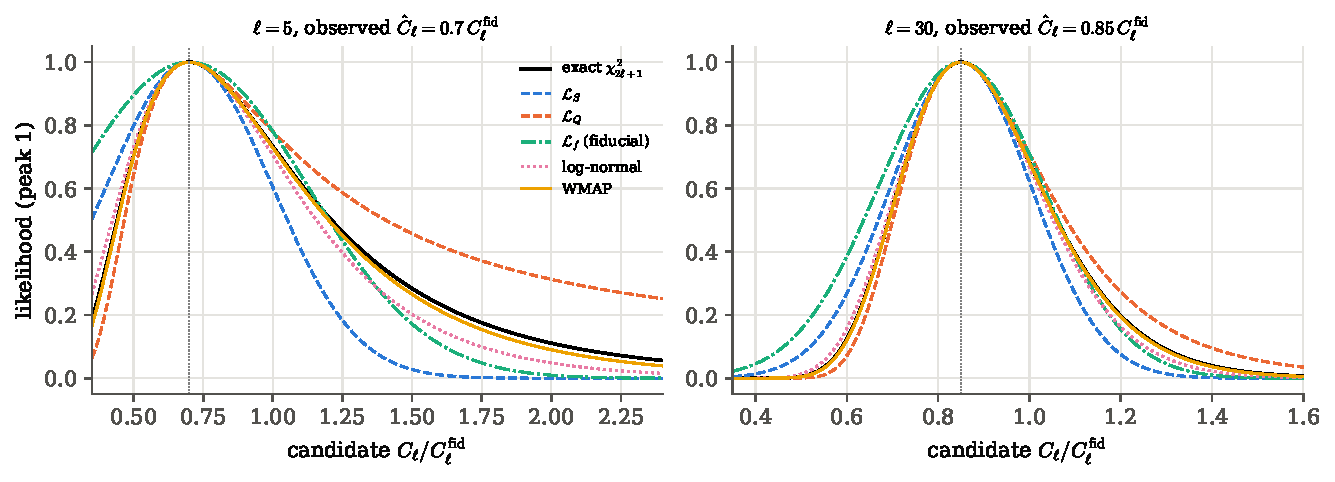
\includegraphics[width=0.92\linewidth]{figures/ch09/cl_like_shapes.pdf}
\caption{Likelihood of the true spectrum, in units of a fiducial one, after observing
$\Chat=0.7\,C^{\rm fid}_\ell$ at $\ell=5$ (left) and $0.85\,C^{\rm fid}_\ell$ at $\ell=30$ (right). The exact
likelihood (black) peaks at the observed value with a long tail to the right. The symmetric
approximation $\Like_S$ is too narrow on the high side; $\Like_Q$ has far too heavy a tail there (it tends to
a constant as $\Cell$ grows); the fixed-fiducial $\Like_f$ is symmetric; the WMAP combination is close to
exact. At $\ell=30$ all forms agree better: the
distribution of $\Chat$ becomes Gaussian as $\ell$ grows.}
\label{9c:fig:cl-shapes}
\end{figure}

\subsection{Reproducing Hamimeche and Lewis, Fig.~1}
\label{9c:sec:hl}

\paragraph{Their question.} In 2008, with Planck about to fly, every high-$\ell$ CMB analysis used one of the
Gaussian shortcuts of \cref{9c:sec:cl-approx}, because the exact likelihood cannot be evaluated on a masked
sky. Hamimeche and Lewis asked which of them is safe \cite{HamimecheLewis2008}: which ones return the same
spectrum as the exact likelihood, to within an error small enough not to matter at Planck's precision? The
cost of a wrong answer is a biased parameter: as the previous example showed, a bias that depends on $\ell$
reads as a tilt, and for $\Like_Q$ it moves $n_s$ by about one standard deviation.

\paragraph{Their setup, one item at a time.}
\emph{The truth.} A fiducial spectrum $C^{\rm f}_\ell$, and many simulated full, noiseless skies drawn from it.
On the full sky the exact likelihood is known, so each approximation can be compared with it sky by sky.
\emph{The test statistic.} The data are cut into bins of ten multipoles, $\ell_{\min}\le\ell\le\ell_{\min}+9$, and in
each bin one amplitude is fitted, $\Cell=AC^{\rm f}_\ell$, by maximising the exact likelihood and each
approximation in turn. An amplitude is the simplest parameter that a bias in the spectrum can move.
\emph{Bias and scatter.} For approximation $i$, the bias is the mean of $A_i-A_{\rm exact}$ over the simulated
skies, and the scatter is the root-mean-square of the same difference. The bias says whether the
approximation is systematically off; the scatter says how far it is off on a typical sky.
\emph{The tolerance.} An error matters only if it is comparable with the cosmic-variance error of the
amplitude itself. For an amplitude fitted to all multipoles up to $\ell$, the exact $\hat A=\sum\nu x_\ell/\sum\nu$
has variance $\sum\nu^2(2/\nu)/(\sum\nu)^2=2/\sum\nu$, and $\sum_{\ell'=2}^{\ell}(2\ell'+1)=(\ell+1)^2-4\approx\ell^2$, so
its error is about $\sqrt2/\ell$. HL take $1/\ell_{\min}$ as the line below which a bias in one bin is harmless
(their eqs.~19--20).

\paragraph{Their key equations.} The exact best fit and the best fits of the approximations are those derived
in \cref{9c:sec:cl-approx}: $\hat A=\sum\nu x_\ell/\sum\nu$ for the exact likelihood and for $\Like_f$, and
$\hat A_Q=\sum\nu x_\ell^2/\sum\nu x_\ell$ for $\Like_Q$, whose bias is \eqref{9c:eq:AQ-bias} (HL eqs.~17--20). The
symbols map directly: $x_\ell$ is the ratio $\Chat/C^{\rm f}_\ell$ of the simulated to the fiducial spectrum,
$\nu=2\ell+1$ the number of modes at $\ell$ on the full sky, and $L=10$ the width of a bin.

\paragraph{What we compute.} Only $x_\ell$ matters, and $\nu x_\ell\sim\chi^2_\nu$ exactly
(\eqref{9c:eq:chat-law}), so we draw the $x_\ell$ directly from $\chi^2$ distributions, $\NineCHLnsim$
realisations per bin as in the paper, for 70 values of $\ell_{\min}$ between 2 and 1500. The best fits of
$\Like_S$, $\Like_Q$ and the log-normal have closed forms; for Gaussian$_D$, WMAP and the cube-root form we use a
vectorised golden-section search, as HL did. The likelihood functions are:
\pyfile[firstline=34,lastline=59]{code/ch09/42_cl_likelihoods.py}{The exact likelihood and its approximations at one multipole}
For the published curves we read the vector paths of HL's Fig.~1 directly from the PDF and convert them
to data coordinates with the tick marks.

\paragraph{Side by side.} \Cref{9c:fig:hl} overlays the two, and the table compares them at
$\ell_{\min}=\NineCHLlref$ (and the scatter also at $\ell_{\min}=\NineCHLlrefHund$):
\begin{center}
\small
\renewcommand{\arraystretch}{1.15}
\begin{tabular}{@{}lcccc@{}}
\toprule
 & \multicolumn{2}{c}{bias $\abs{\langle A_i-A_{\rm exact}\rangle}$} & \multicolumn{2}{c}{scatter $\langle(A_i-A_{\rm exact})^2\rangle^{1/2}$}\\
 & HL Fig.~1 & ours & HL Fig.~1 & ours ($\ell_{\min}=\NineCHLlrefHund$)\\\midrule
$\Like_S$ & $\NineCHLpubBiasS$ & $\NineCHLbiasS$ & $\NineCHLpubRmsS$ & $\NineCHLrmsS$ ($\NineCHLrmsSHund$)\\
$\Like_Q$ & $\NineCHLpubBiasQ$ & $\NineCHLbiasQ$ & $\NineCHLpubRmsQ$ & $\NineCHLrmsQ$ ($\NineCHLrmsQHund$)\\
Gaussian$_D$ & $\NineCHLpubBiasD$ & $\NineCHLbiasD$ & $\NineCHLpubRmsD$ & $\NineCHLrmsD$ ($\NineCHLrmsDHund$)\\
WMAP & noise & $\NineCHLbiasWMAP$ & $\NineCHLpubRmsWMAP$ & $\NineCHLrmsWMAP$ ($\NineCHLrmsWMAPHund$)\\
cube root & noise & $\NineCHLbiasCube$ & $\NineCHLpubRmsCube$ & $\NineCHLrmsCube$ ($\NineCHLrmsCubeHund$)\\
\bottomrule
\end{tabular}
\end{center}
In units of $1/\ell$ the biases are $\NineCHLSoverL$ ($\Like_S$, outside the tolerance), $\NineCHLQoverL$
($\Like_Q$, as predicted by \eqref{9c:eq:AQ-bias}) and $\NineCHLDoverL$ (Gaussian$_D$).

\paragraph{Why they differ.}
\begin{enumerate}[itemsep=1pt]
  \item \emph{Reading precision.} The symmetric Gaussian, the quadratic form and Gaussian$_D$ agree with the paper
        to a few per cent, which is the precision of reading a curve off a plot.\footnote{For Gaussian$_D$ we used
        HL's eq.~(25) as printed, $\Like_Q$ plus $\ln\Cell$ once per multipole; this is the form that reproduces
        their curve.}
  \item \emph{Monte Carlo noise.} The WMAP and cube-root biases are of order $10^{-7}$. A mean of $10^4$ differences
        whose scatter is a few times $10^{-6}$ has a Monte Carlo error of $4\times10^{-6}/\sqrt{10^4}=4\times10^{-8}$,
        so these biases are that noise: both curves, the paper's and ours, jitter because they measure nothing
        but the random draws. The scatter of the WMAP form matches.
  \item \emph{An unspecified variant.} Our cube-root scatter, $\NineCHLrmsCube$, is about half the published
        $\NineCHLpubRmsCube$. HL plot the cube-root form without saying which of their two variants ($\alpha=\pm1$
        in eq.~28) is shown, and we used $\alpha=-1$. Either way it is three orders of magnitude inside the
        tolerance, and the conclusion is the same.
\end{enumerate}
\emph{A final check.} HL's own new approximation (their eqs.~41--50) is built on
$g(x)=\mathrm{sign}(x-1)\sqrt{2(x-\ln x-1)}$, with $x=\Chat/\Cell$ the ratio to the model. By
\eqref{9c:eq:exact-u} with $1+u=x$, the exact $-2\ln\Like$ minus its minimum is $\nu[(x-1)-\ln x]=\nu(x-\ln x-1)$,
and $g(x)^2=2(x-\ln x-1)$, so
\[
  -2\ln\Like_{\rm exact}=\tfrac\nu2\,g(x)^2 .
\]
On the full sky the exact likelihood is therefore a Gaussian in the variable $g$, with variance $2/\nu$: the
same quadratic shape as the shortcuts, but in a variable chosen so that it is exact. On a cut sky the variance
$2/\nu$ is replaced by a covariance of the $g$ values measured on simulations, as for the other forms. Our best
fits with it equal the exact ones to $\NineCHLcheck$, the precision of the search.

\paragraph{The lesson.} All the shortcuts are right at the peak; what separates safe from unsafe is the cubic
term, and the ``biases'' of the safe ones in the published figure are Monte Carlo noise, which only rerunning
the test reveals.

\begin{figure}[htbp]
\centering
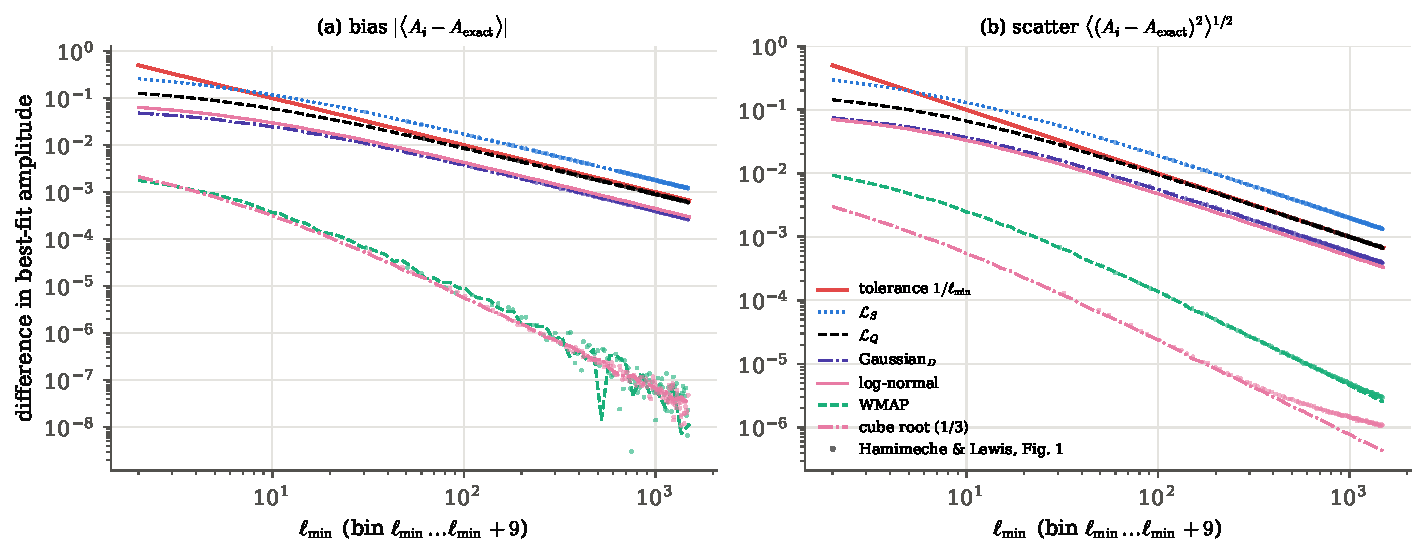
\includegraphics[width=\linewidth]{figures/ch09/hl_fig1.pdf}
\caption{Reproduction of Fig.~1 of Hamimeche and Lewis. For bins of ten multipoles starting at
$\ell_{\min}$, the bias (a) and the scatter (b) of the best-fit amplitude under each approximation,
relative to the exact likelihood, from $10^4$ simulated full skies per bin (lines), with the curves read
from the published figure (dots) and the tolerance $1/\ell_{\min}$ (red). The symmetric $\Like_S$ fails;
$\Like_Q$ sits on the tolerance; WMAP and the cube-root forms are far inside, and their biases are Monte
Carlo noise.}
\label{9c:fig:hl}
\end{figure}

\paragraph{What Planck does.} The Planck 2018 temperature likelihood is a hybrid split at $\ell=30$
\cite{Planck2018V}. Below it, where the skewness of \cref{9c:fig:cl-shapes} is large, Planck uses the exact
likelihood in a form that survives the mask and the noise \cite{Chu2005}. Call $\bm s$ the full-sky signal, the
sky we would see with no mask and no noise, and $\bm d$ the masked, noisy data. If we knew $\bm s$ the problem
would be the one already solved: its spectrum, which we call $\sigma_\ell$ (the spectrum of a full sky, as $\Chat$
was), would enter \eqref{9c:eq:exact-like}. We do not know $\bm s$, so we average over what the data allow it to be.
With a flat prior on $\Cell$,
\begin{align}
  p(\Cell\given\bm d)
  &\eqby{1}\int p(\Cell\given\bm s,\bm d)\,p(\bm s\given\bm d)\,\dd\bm s
   \eqby{2}\int p(\Cell\given\bm s)\,p(\bm s\given\bm d)\,\dd\bm s
   \nonumber\\
  &\eqby{3}\frac1{N_{\rm G}}\sum_{i=1}^{N_{\rm G}}p(\Cell\given\bm s^i)
   \eqby{4}\frac1{N_{\rm G}}\sum_{i=1}^{N_{\rm G}}\prod_{\ell=2}^{29}\frac{\text{const}}{\sigma^i_\ell}
   \Bigl(\frac{\sigma^i_\ell}{\Cell}\Bigr)^{\nu/2}e^{-\nu\sigma^i_\ell/2\Cell}.
  \label{9c:eq:blackwell-rao}
\end{align}
\begin{explain}
  \item The full sky is an unknown intermediate; marginalise it, with the product rule.
  \item Once the full sky is known, the masked and noisy data add nothing about its spectrum.
  \item Replace the integral over $p(\bm s\given\bm d)$ by an average over $N_{\rm G}$ samples $\bm s^i$ drawn from it;
        the average approaches the integral as $N_{\rm G}$ grows (\cref{9a:sec:ergodic}).
  \item $p(\Cell\given\bm s)$ depends on $\bm s$ only through its spectrum $\sigma_\ell$, so it is
        \eqref{9c:eq:exact-like} with $\Chat\to\sigma^i_\ell$ and $\nu=2\ell+1$, normalised over $\Cell$: the integral
        $\int\Cell^{-\nu/2}e^{-\nu\sigma/2\Cell}\dd\Cell$ is proportional to $\sigma^{1-\nu/2}$ by line~1 of
        \eqref{9c:eq:invgamma-mean}, so the normalised density carries the factor $\sigma^{\nu/2-1}$, which is
        written as $(1/\sigma)\,\sigma^{\nu/2}$. Different $\ell$ are independent given $\bm s$.
\end{explain}
The samples $\bm s^i$ come from a Gibbs sampler (\cref{9b:sec:gibbs}) that alternates between drawing a full sky
given the data and the current spectrum, and drawing a spectrum given that sky; each $\bm s^i$ is one full sky
compatible with the masked, noisy map, and $\sigma^i_\ell$ is its spectrum. The last line is Planck 2018 V, eq.~2,
the Blackwell--Rao estimator: the exact full-sky likelihood averaged over what the mask and the noise hide. The
factor $(\sigma^i_\ell)^{\nu/2-1}$, which a single sky could drop because it does not depend on $\Cell$, now
matters, because it differs from sample to sample. Above
$\ell=30$ Planck uses a Gaussian in the cross-spectra with a covariance computed for a fixed fiducial model
(their eq.~20): the multi-field, cut-sky version of $\Like_f$. Their footnote~12 records that the symmetric shape
biases $n_s$ by about $0.1\sigma$, and that they ignore it. \Cref{9c:sec:planck-gauss} measures the bias of this
choice in our idealised setting.
\section{A model spectrum fast enough for a chain}
\label{9c:sec:emu}

Equation \eqref{9c:eq:hier} says that every step of the chain needs the spectrum $\Cell(\params)$ at the
proposed parameters. The honest way to get it is a Boltzmann code. CAMB \cite{CAMB2000} computes a
lensed temperature spectrum to $\ell=2500$ in about $\NineCEmuTcamb$\,s on the laptop. A run of four
chains of $40\,000$ steps, the size used in \cref{9c:sec:planck}, would then take some forty hours, and the
whole point of a chain is that it can be rerun when something changes. Research codes pay this price on a
cluster (\cref{9c:sec:research}). We replace the Boltzmann code by an \newterm{emulator} \unpack{a cheap
function that reproduces the code's output over the region of parameter space the chain will visit},
built once from a few dozen CAMB calls and checked against CAMB before it is trusted.

\paragraph{The question.} How do we build a function that returns $\Cell(\params)$ in microseconds, and how
do we know it is accurate enough? ``Accurate enough'' has a precise meaning: the emulator's error must
change $-2\ln\Like$ by much less than one anywhere the posterior has weight, because a change of one in
$-2\ln\Like$ is what moves a parameter by one standard deviation.

\subsection{Expand the logarithm}
\label{9c:sec:emu-log}

We use a Taylor series around the fiducial Planck 2018 model $\params_0$, in six parameters
$\params=(\ln10^{10}A_s,\,n_s,\,H_0,\,\omega_b,\,\omega_c,\,\tau)$. The first two describe the primordial
fluctuations: $A_s$ is their amplitude at the pivot wavenumber $k_*$ and $n_s$ their tilt, how that amplitude
changes with scale (\cref{8a:sec:lit-pivot}). $H_0$ is the present expansion rate. $\omega_b=\Omega_bh^2$ and
$\omega_c=\Omega_ch^2$ are the physical densities of baryons and of cold dark matter, their density
parameters times $h^2$ with $h=H_0/(100\,\mathrm{km\,s^{-1}\,Mpc^{-1}})$, which fix their actual mass per unit
volume. $\tau$ is the optical depth to reionisation: a CMB photon scatters off a free electron after the
Universe was reionised with probability $1-e^{-\tau}\approx\tau$. The fiducial values, those of CAMB's input everywhere in the book,
are
\begin{center}
\small
\renewcommand{\arraystretch}{1.15}
\begin{tabular}{@{}cccccc@{}}
\toprule
$\ln(10^{10}A_s)$ & $n_s$ & $H_0$ (km\,s$^{-1}$\,Mpc$^{-1}$) & $\omega_b$ & $\omega_c$ & $\tau$\\\midrule
$3.044$ & $0.9649$ & $67.36$ & $0.02237$ & $0.1200$ & $0.0544$\\
\bottomrule
\end{tabular}
\end{center}
with $A_s=2.100\times10^{-9}$ at $k_*=0.05$\,Mpc$^{-1}$. The question is: a series for what?
Look at how the parameters enter. The primordial power is $P(k)=A_s(k/k_*)^{n_s-1}$ with the pivot
$k_*=0.05$\,Mpc$^{-1}$, and the spectrum is a weighted integral of it, $\Cell=\int\dd k\,T(\ell,k)\,P(k)$
with a transfer function $T\ge0$ (the scalar term of the cosmology notes' $\sum_m\int T_mP_m$). Reionisation
multiplies the spectrum at $\ell\gg10$ by $e^{-2\tau}$ (cosmology notes). So, writing $x=\ln(k/k_*)$,
\begin{align}
  \ln\Cell
  &\eqby{1}\ln A_s-2\tau+\ln\int\dd k\,T(\ell,k)\,e^{(n_s-1)x},
  \nonumber\\
  \frac{\partial\ln\Cell}{\partial n_s}
  &\eqby{2}\frac{\int\dd k\,T\,e^{(n_s-1)x}\,x}{\int\dd k\,T\,e^{(n_s-1)x}}\equiv\langle x\rangle_\ell,
  \qquad
  \frac{\partial^2\ln\Cell}{\partial n_s^2}\eqby{3}\langle x^2\rangle_\ell-\langle x\rangle_\ell^2\ge0 .
  \label{9c:eq:dlnC}
\end{align}
\begin{explain}
  \item $A_s$ and $e^{-2\tau}$ are overall factors (for $\ell\gg10$, ignoring lensing, which depends weakly
        on $A_s$ too), and $(k/k_*)^{n_s-1}=e^{(n_s-1)x}$.
  \item Differentiate the logarithm of the integral: the derivative of the exponent brings down $x$. The
        ratio is the average of $x$ over the normalised weight $T\,e^{(n_s-1)x}$, the range of
        wavenumbers that feed multipole $\ell$.
  \item Differentiate the ratio once more (quotient rule): the result is the variance of $x$ under the
        same weight.
\end{explain}
So $\ln\Cell$ is exactly linear in $\ln A_s$ and $\tau$, and nearly linear in $n_s$: its curvature in $n_s$
is the variance of $\ln k$ over the wavenumbers that contribute to one multipole, a small number. The
spectrum itself is \emph{not} linear in these parameters ($\Cell\propto A_s$ is linear, but $e^{-2\tau}$ and
$e^{(n_s-1)x}$ are not). The expansion we use is therefore
\begin{equation}
  \ln\Cell(\params)\simeq\ln\Cell(\params_0)+\sum_iD_{i\ell}\,\delta\theta_i
  +\tfrac12\sum_{ij}H_{ij\ell}\,\delta\theta_i\delta\theta_j,
  \qquad D_{i\ell}=\frac{\partial\ln\Cell}{\partial\theta_i},\quad H_{ij\ell}=\frac{\partial^2\ln\Cell}{\partial\theta_i\partial\theta_j},
  \label{9c:eq:emu}
\end{equation}
at first or second order, with all derivatives at $\params_0$.

\paragraph{Example: the derivatives read as physics.} CAMB gives, by central differences,
$\partial\ln\Cell/\partial\tau=\NineCEmuDtauHigh$ averaged over $500\le\ell\le2000$: the factor $e^{-2\tau}$
exactly. It gives $\partial\ln\Cell/\partial n_s=\NineCEmuDnThousand$ at $\ell=1000$ and $\NineCEmuDnTen$ at
$\ell=10$; by \eqref{9c:eq:dlnC} these are average values of $\ln(k/k_*)$, so multipole 1000 is fed by
wavenumbers about $e^{0.55}\approx1.7$ times the pivot and multipole 10 by wavenumbers some forty times
smaller. Somewhere between, at a multipole of a few hundred, the average is zero: that multipole sees the
pivot, and changing $n_s$ leaves it unchanged, which is the meaning of the pivot (\cref{ch:08}). The second
derivative at $\ell=1000$ is $\NineCEmuHnn$, a spread of about $0.3$ in $\ln k$. The second derivative in
$\ln A_s$ is at most $\NineCEmuHAA$ for $30\le\ell\le2000$: it would be zero without lensing, whose strength
also grows with $A_s$. \Cref{9c:fig:emu-derivs} plots all six first derivatives, each multiplied by that
parameter's expected error so that the curves show how much one standard deviation of each parameter
changes the spectrum.

\begin{figure}[htbp]
\centering
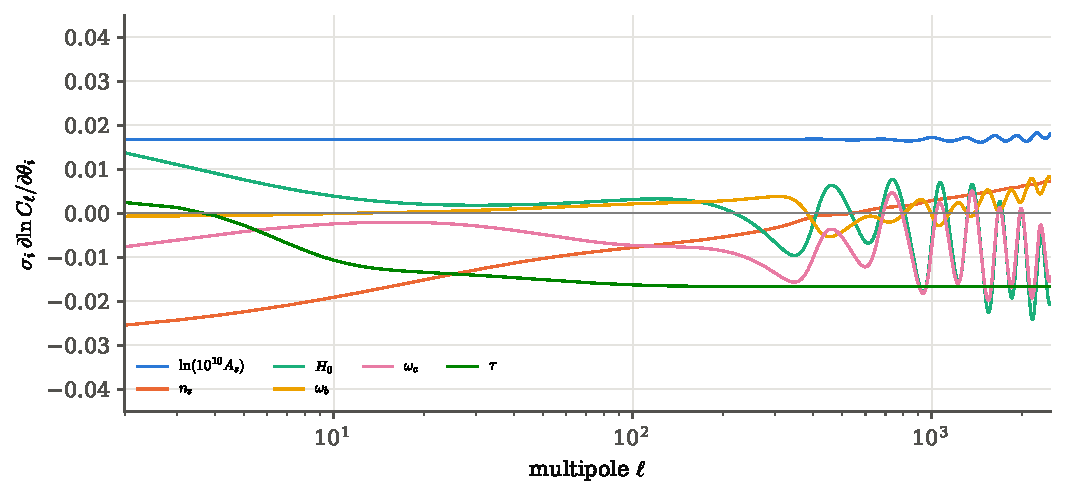
\includegraphics[width=0.85\linewidth]{figures/ch09/emu_derivs.pdf}
\caption{What one standard deviation of each parameter does to $\ln\Cell$. The amplitude (blue) and the
optical depth (dark green) give flat, opposite responses above $\ell\approx30$: a temperature spectrum
alone cannot separate them. The tilt $n_s$ (orange) rotates the spectrum about a multipole of several
hundred. $H_0$, $\omega_b$ and $\omega_c$ move and reshape the acoustic peaks, hence the oscillations.}
\label{9c:fig:emu-derivs}
\end{figure}

\subsection{Building it}
\label{9c:sec:emu-build}

The derivatives come from central differences. For one parameter with step $h$,
$f(\theta\pm h)=f\pm hf'+\tfrac12h^2f''\pm\tfrac16h^3f'''+\dots$, so
\begin{align}
  \frac{f(\theta+h)-f(\theta-h)}{2h}\eqby{1}f'+\tfrac16h^2f''',
  \qquad
  \frac{f(\theta+h)-2f(\theta)+f(\theta-h)}{h^2}\eqby{2}f''+\tfrac1{12}h^2f'''' ,
  \label{9c:eq:central}
\end{align}
\begin{explain}
  \item Subtract the two series: even powers cancel.
  \item Add them: odd powers cancel.
\end{explain}
both with errors of order $h^2$. Mixed second derivatives use the four corners
$(\pm h_i,\pm h_j)$. For $d=6$ parameters that is $1+2d+4\binom d2=\NineCEmuBuildCalls$ CAMB calls, about a
minute; the steps ($0.02$ in $\ln10^{10}A_s$, $0.01$ in $n_s$, $0.5$ in $H_0$, $0.0003$ in $\omega_b$, $0.003$ in
$\omega_c$, $0.01$ in $\tau$) are those of the finite-difference study of \cref{ch:08}. Evaluating the
emulator is two small matrix products:
\pyfile[firstline=93,lastline=102]{code/ch09/lib_cmbemu.py}{The emulator: ln C to first or second order}
It takes $\NineCEmuTemu\,\mu$s, $\NineCEmuSpeedup$ times faster than CAMB, which turns forty hours of chain
into a few seconds.

\subsection{How accurate is accurate enough?}
\label{9c:sec:emu-check}

To check the emulator we need the scale on which it must be right, and that scale is set by the data. Our
target experiment is Planck-like: one channel with a $7.22'$ Gaussian beam and white noise of
$33\,\mu$K\,arcmin, the 143\,GHz values of Planck 2018 \cite{Planck2018I}, on $\fsky=\NineCEmuFsky$ of the sky,
$2\le\ell\le2500$. Its noise power, deconvolved by the beam, is
$N_\ell=\Delta_T^2\,e^{\ell(\ell+1)\sigma_b^2}$, with $\Delta_T$ the depth in $\mu$K\,rad and
$\sigma_b=\mathrm{FWHM}/\sqrt{8\ln2}$ (\cref{ch:08}). How far does a model error $\delta\Cell$ move $-2\ln\Like$?
Expand the exact likelihood \eqref{9c:eq:exact-like}, with $\Cell\to\Cell+N_\ell$ and $\nu=(2\ell+1)\fsky$, about
the true spectrum and average over data; at one multipole, with $\mathcal C=\Cell+N_\ell$,
\begin{align}
  \E\Bigl[-2\ln\Like(\mathcal C+\delta C)\Bigr]-\E\Bigl[-2\ln\Like(\mathcal C)\Bigr]
  &\eqby{1}\nu\Bigl[\frac{\mathcal C}{\mathcal C+\delta C}+\ln(\mathcal C+\delta C)-1-\ln\mathcal C\Bigr]
   \nonumber\\
  &\eqby{2}\nu\Bigl[-\epsilon+\epsilon^2+\epsilon-\tfrac12\epsilon^2+O(\epsilon^3)\Bigr]
   \eqby{3}\frac\nu2\Bigl(\frac{\delta C}{\Cell+N_\ell}\Bigr)^2+O(\epsilon^3),
  \label{9c:eq:dchi2}
\end{align}
\begin{explain}
  \item $\E\Chat=\mathcal C$ (the estimator is unbiased), so the data enter only through their mean.
  \item With $\epsilon=\delta C/\mathcal C$: $1/(1+\epsilon)=1-\epsilon+\epsilon^2-\dots$ and
        $\ln(1+\epsilon)=\epsilon-\epsilon^2/2+\dots$.
  \item The linear terms cancel, because the true spectrum maximises the expected likelihood.
\end{explain}
Summed over $\ell$ this is $\Delta\chi^2=\sum_\ell\frac\nu2[\delta\Cell/(\Cell+N_\ell)]^2$, the change of $-2\ln\Like$
that the emulator error alone produces. The same expansion measures a change of parameters. A small step
$\delta\params$ changes the spectrum by $\delta\Cell=\sum_i\partial_i\Cell\,\delta\theta_i$, with
$\partial_i\equiv\partial/\partial\theta_i$, and substituting it,
\begin{align}
  \Delta\chi^2
  &\eqby{1}\sum_\ell\frac\nu2\Bigl(\sum_i\frac{\partial_i\Cell\,\delta\theta_i}{\Cell+N_\ell}\Bigr)^2
   \eqby{2}\sum_{ij}\delta\theta_i\,\delta\theta_j\sum_\ell\frac\nu2\,\frac{\partial_i\Cell\,\partial_j\Cell}{(\Cell+N_\ell)^2}
   \eqby{3}\delta\params\T\Fish\,\delta\params ,
  \label{9c:eq:dchi2-fisher}
\end{align}
\begin{explain}
  \item \eqref{9c:eq:dchi2} with $\delta C=\sum_i\partial_i\Cell\,\delta\theta_i$.
  \item The square of a sum is a double sum, $(\sum_ia_i)^2=\sum_{ij}a_ia_j$; the $\delta\theta$ do not depend on
        $\ell$ and come out of the sum over $\ell$.
  \item Name the inner sum $F_{ij}$.
\end{explain}
with the \newterm{Fisher matrix}
\begin{equation}
  F_{ij}=\sum_\ell\frac{(2\ell+1)\fsky}{2}\,\frac{\partial_i\Cell\,\partial_j\Cell}{(\Cell+N_\ell)^2}
  \;\Bigl[+\frac{1}{\sigma_\tau^2}\ \text{for}\ i=j=\tau\Bigr],
  \label{9c:eq:fisher-cl}
\end{equation}
which \cref{ch:10} develops in full. The bracket is the Gaussian prior on $\tau$, of width
$\sigma_\tau=\NineCEmuSigTauPrior$, that stands in for Planck's low-$\ell$ polarization (``lowE'') measurement
\cite{Planck2018VI}. A Gaussian prior adds $(\tau-\tau_{\rm obs})^2/\sigma_\tau^2$ to $-2\ln\Like$; a step
$\delta\tau$ raises that term by $\delta\tau^2/\sigma_\tau^2$, which is $\delta\params\T\Fish\,\delta\params$ with
$1/\sigma_\tau^2$ added to $F_{\tau\tau}$ alone. Without the prior a temperature spectrum cannot separate $A_s$ from
$\tau$ (\cref{9c:fig:emu-derivs}). The posterior near its peak is then $\propto e^{-\delta\params\T\Fish\delta\params/2}$, a
Gaussian with covariance $\Fish^{-1}$, so the error of parameter $i$ with all the others free is
$\sigma_i=\sqrt{(\Fish^{-1})_{ii}}$, not $1/\sqrt{F_{ii}}$; the second is the error with all the others held fixed, and
the two differ whenever parameters are correlated (\cref{10a:sec:marginal}, \eqref{10a:eq:marg-cond}). Holding
fixed a parameter that is in fact unknown is what produces the factor of nine in $\ln(10^{10}A_s)$ of
\cref{9c:sec:planck}.
The expected errors $\sigma_i$ set the natural size of a
step: $\NineCEmuSigLnAs$ in $\ln10^{10}A_s$, $\NineCEmuSigNs$ in $n_s$, $\NineCEmuSigHzero$ in $H_0$,
$\NineCEmuSigOmb$ in $\omega_b$, $\NineCEmuSigOmc$ in $\omega_c$ and $\NineCEmuSigTau$ in $\tau$. With only
$(\ln10^{10}A_s,n_s)$ free and the rest fixed, $F$ is the $2\times2$ corner and the errors shrink to
$\NineCEmuSigLnAsTwo$ and $\NineCEmuSigNsTwo$, with correlation $\NineCEmuRhoTwo$; we return to these numbers in
\cref{9c:sec:planck}.

Now the test. We compare three emulators, the series in $\Cell$ itself to first order, the series in
$\ln\Cell$ to first order, and the series in $\ln\Cell$ to second order, against direct CAMB calls, at two kinds
of points: along each parameter axis at $\pm1$, $\pm3$ and $\pm5\sigma_i$, and at $\NineCEmuNrand$ random points
drawn from the Fisher Gaussian with its widths doubled, which reach out to $\NineCEmuMaxDist\sigma$ from the
fiducial.
\begin{center}
\small
\renewcommand{\arraystretch}{1.15}
\begin{tabular}{@{}lcccc@{}}
\toprule
$\Delta\chi^2$ from the emulator error & axes, $\pm1\sigma$ (max) & axes, $\pm5\sigma$ (max) & random (median) & random (max)\\\midrule
first order in $\Cell$ & $\NineCEmuCutOneLinC$ & $\NineCEmuCutFiveLinC$ & $\NineCEmuMedLinC$ & $\NineCEmuMaxLinC$\\
first order in $\ln\Cell$ & $\NineCEmuCutOneLin$ & $\NineCEmuCutFiveLin$ & $\NineCEmuMedLin$ & $\NineCEmuMaxLin$\\
second order in $\ln\Cell$ & $\NineCEmuCutOneQuad$ & $\NineCEmuCutFiveQuad$ & $\NineCEmuMedQuad$ & $\NineCEmuMaxQuad$\\
\bottomrule
\end{tabular}
\end{center}
With six free parameters the first-order series are not good enough: at $5\sigma$ along one axis they are
wrong by tens in $\chi^2$, and at random points within the posterior they reach $\Delta\chi^2\approx2$. Their
errors oscillate with the acoustic peaks (\cref{9c:fig:emu-check}a): $H_0$, $\omega_b$ and $\omega_c$ move the peaks
sideways, and a sideways shift of an oscillating function is not linear in the size of the shift. The second-order series in $\ln\Cell$ stays below $\Delta\chi^2=0.1$
everywhere we tested (\cref{9c:fig:emu-check}b). With only $(\ln10^{10}A_s,n_s)$ free, for which \eqref{9c:eq:dlnC}
promised near-linearity, the first-order series in $\ln\Cell$ is already enough: its worst error at the
four corners $(\pm5\sigma,\pm5\sigma)$ is $\Delta\chi^2=\NineCEmuTwoWorst$. These are the two emulators we use:
first order for two or three parameters, second order for six.

\begin{figure}[htbp]
\centering
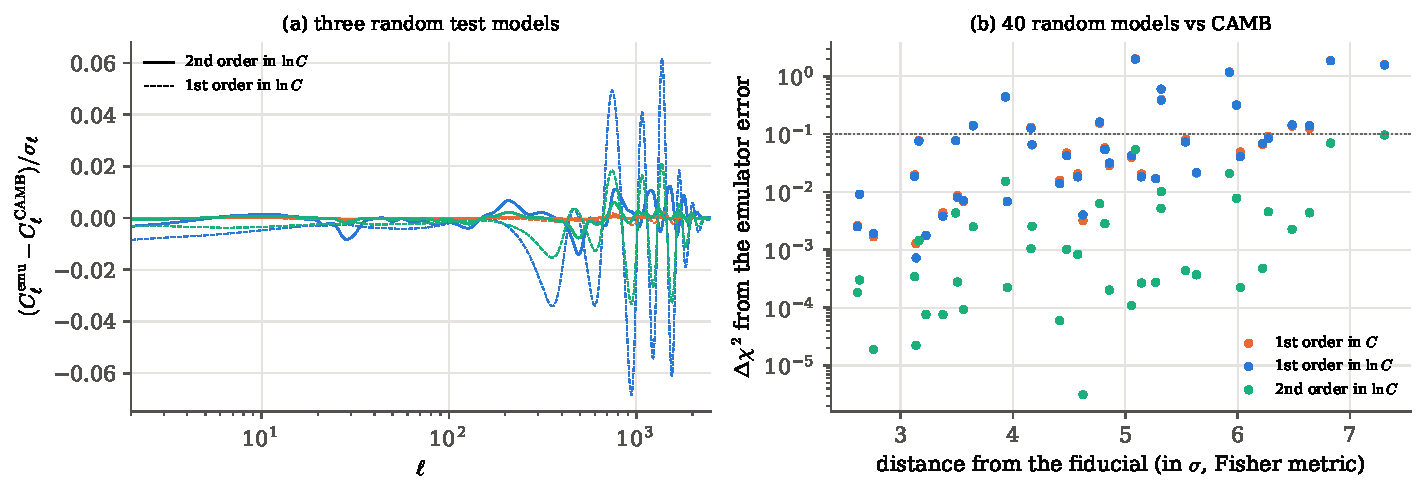
\includegraphics[width=\linewidth]{figures/ch09/emu_check.pdf}
\caption{Testing the emulator against CAMB. (a) For three random models, the emulator error at each $\ell$ in
units of the error bar of one multipole: second order in $\ln\Cell$ (solid) against first order (dotted); the
first-order errors oscillate with the acoustic peaks. (b) The $\Delta\chi^2$ produced by the emulator error at
40 random models, against their distance from the fiducial; the dotted line is $\Delta\chi^2=0.1$.}
\label{9c:fig:emu-check}
\end{figure}

\paragraph{Example: what $\Delta\chi^2=0.1$ does to a posterior.} An error $\Delta\chi^2$ in $-2\ln\Like$
multiplies the posterior density at that point by $e^{-\Delta\chi^2/2}$. If the error were a constant, it would
cancel in the normalisation; what matters is how it varies across the posterior. Errors that vary by $0.1$
across the posterior reweight its regions by at most $e^{0.05}\approx1.05$: a five per cent reweighting of
the tails, which moves means by a few hundredths of a standard deviation. \Cref{9c:sec:importance} measures
this directly by reweighting the six-parameter chain with CAMB itself.

\paragraph{Laptop versus research.} Our emulator costs 73 Boltzmann calls and is valid only within a few
standard deviations of the fiducial model; it could not explore a prior much wider than the posterior or a
cosmology far from Planck's. Research analyses either call CAMB or CLASS at every step, with the fast and
slow parameters of \cref{9b:sec:relatives} updated at different rates \cite{LewisBridle2002}, or train a
neural-network emulator on $10^5$ Boltzmann runs spread over the whole prior, as CosmoPower does
\cite{SpurioMancini2022}. Either way the principle is the one used here: validate the fast model against the
slow one on the posterior itself.
\section{Cosmological parameters from one simulated sky}
\label{9c:sec:toy}

\Cref{ch:08} built a small CMB experiment on the laptop and studied what it does to the power spectrum: a
$30'$ beam, white noise of $200\,\mu$K\,arcmin, maps at HEALPix resolution $N_{\rm side}=256$, and a Galactic
band $|b|<20^\circ$ masked with edges tapered over $5^\circ$. It produced the sampling distribution of the
measured spectrum, including a covariance of the masked bandpowers from 2000 simulated skies. Everything
needed for inference is now in place: the likelihood (\cref{9c:sec:cl-like}), a fast model
(\cref{9c:sec:emu}), and the sampler. We take one simulated sky, observe it three ways, and ask what each
observation says about two parameters of the primordial spectrum, the amplitude $\ln(10^{10}A_s)$ and the
tilt $n_s$, with the other four $\Lambda$CDM parameters held at their true values.

\paragraph{The question.} The reasoning is that of \cref{9c:sec:cl-like}: every candidate pair of amplitude and
tilt is a hypothesis about the sky, and the measured spectrum is asked how probable it would have been under
each. How does the posterior of $(\ln10^{10}A_s,n_s)$ change from (a) a perfect,
noiseless view of the whole sky, to (b) the same sky seen through the beam and the noise, to (c) the noisy
sky behind the Galactic mask? And are the chains' answers the ones the Fisher matrix predicts?

\subsection{One sky, three observations, three likelihoods}
\label{9c:sec:toy-data}

One set of $\alm$ is drawn from the fiducial spectrum up to $\ell=767$, and the analysis uses
$2\le\ell\le\NineCToyLmax$ (\cref{9c:fig:cmb-data}). The three data sets and their likelihoods are:

\emph{(a) The sky itself.} $\Chat$ is the spectrum of the $\alm$ themselves, and the likelihood is the exact
full-sky form \eqref{9c:eq:exact-like} with $\nu=2\ell+1$, summed over $\ell$.

\emph{(b) The full sky with beam and noise.} $\Chat^{\,\rm obs}$ is the spectrum of the observed map, and the
likelihood is the same exact form with the model spectrum replaced by what the instrument should see,
$T_\ell^2\Cell(\params)+N_\ell$, where $T_\ell$ is the beam and pixel window and $N_\ell$ the white-noise power
(\cref{9c:sec:cl-exact}). Nothing is approximated: on the full sky with isotropic noise this is still exact.

\emph{(c) The masked noisy sky.} The data are the $\NineCToyNbins$ MASTER bandpowers $\widehat D_b$ of
\cref{ch:08}, in bins of 20 multipoles, from the masked map ($\fsky=\NineCToyFsky$ of the sky has nonzero
weight). The model predicts them through the bandpower windows, $D_b(\params)=\sum_\ell\mathcal F_{b\ell}\Cell(\params)$,
which encode what the binning, the mask deconvolution and the beam do to a theory spectrum
\cite{Hivon2002}. Their distribution is no longer known exactly, so we use a Gaussian with the covariance
$\widehat{\Cmat}$ measured on the $\NineCToyNsims$ simulations of \cref{ch:08}. That covariance is an unbiased
estimate, but its inverse, which is what the likelihood uses, is not: inverting magnifies the directions in which
the simulations happened to scatter too little, and for $n$ simulations of $p$ bandpowers the inverse comes out
too large on average by the factor $(n-1)/(n-p-2)$ (\cref{8b:sec:hartlap}, \eqref{8b:eq:hartlap-derived}). A
$\chi^2$ built with it would be too large, and the errors too small. We therefore multiply the inverse by the
reciprocal, the Hartlap factor $(n-p-2)/(n-1)=\NineCToyHartlap$ for $n=\NineCToyNsims$ and $p=\NineCToyNbins$
\cite{Hartlap2007}. With two thousand simulations for thirty bins the correction is small: every $\chi^2$ shrinks by
$1.5$ per cent and every error grows by $1/\sqrt{\NineCToyHartlap}\approx1.008$, under one per cent.
The likelihood is

\begin{equation}
  -2\ln\Like=\bigl(\widehat{\bm D}-\bm D(\params)\bigr)\T\,\frac{n-p-2}{n-1}\,\widehat{\Cmat}^{-1}\,\bigl(\widehat{\bm D}-\bm D(\params)\bigr).
  \label{9c:eq:mask-like}
\end{equation}
The covariance is fixed, computed once at the fiducial model: this is the $\Like_f$ of \cref{9c:sec:cl-approx}
on a cut sky, the form Planck uses at high $\ell$. Binning by 20 makes each bandpower an average of about
$20\times(2\ell+1)\fsky$ modes, close to Gaussian except in the first bin or two, where the cost of the
approximation is concentrated.

In code the three log-posteriors are three short functions (the prior is a wide box):
\pyfile[firstline=84,lastline=102]{code/ch09/44_cmb_mcmc.py}{The three likelihoods of the simulated sky}
The model spectrum \pyname{emu.cl} is the first-order series in $\ln\Cell$ in the two free parameters, which
\cref{9c:sec:emu-check} showed to be accurate to $\Delta\chi^2<10^{-4}$ out to five standard deviations.

\begin{figure}[htbp]
\centering
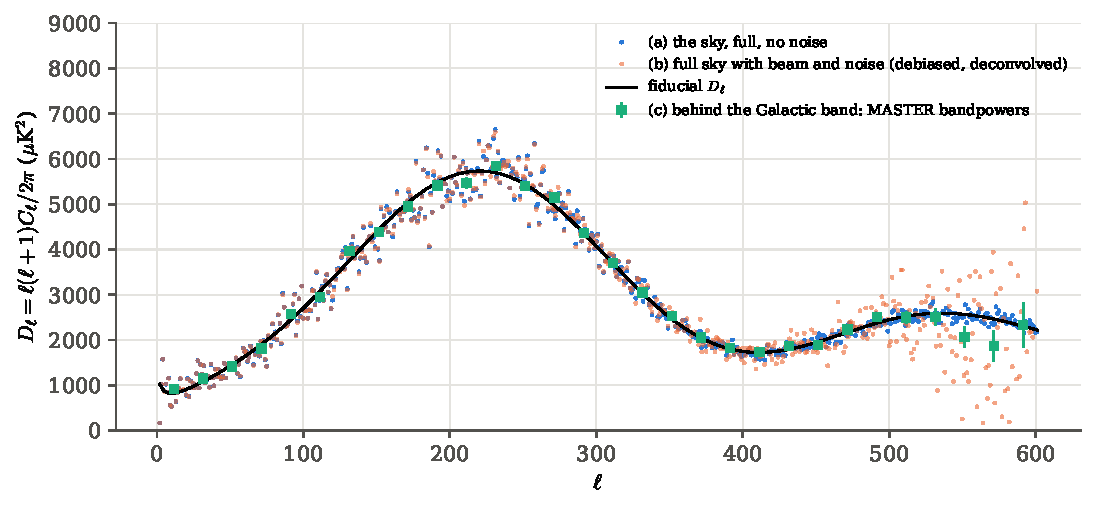
\includegraphics[width=0.88\linewidth]{figures/ch09/cmb_data.pdf}
\caption{The data of the three analyses, as $D_\ell=\ell(\ell+1)\Cell/2\pi$. (a) The spectrum of the simulated
sky itself, scattering about the fiducial model (black) by cosmic variance. (b) The spectrum of the observed
full-sky map, with the noise power subtracted and the beam divided out for display; above $\ell\approx400$
the noise dominates and the scatter grows. (c) MASTER bandpowers from the masked map, with error bars from
the 2000 simulations.}
\label{9c:fig:cmb-data}
\end{figure}

\subsection{The chains and their diagnostics}
\label{9c:sec:toy-chains}

For each case we run $\NineCToyNch$ chains of $\NineCToyNst$ steps, started at random up to six expected
standard deviations from the truth, with the proposal shaped by the Fisher covariance of that case and scaled by
$2.38/\sqrt2$ (\cref{9b:sec:shaped}), and drop $\NineCToyBurn$ steps of burn-in. Each case takes about a second.
Before reading off any number we look at the diagnostic panel that Kruschke recommends
\srcref{Kruschke}{§8.2.5}, here for the masked case (\cref{9c:fig:cmb-diag}): the traces of the four chains
overlap after a few hundred steps; the autocorrelation falls to zero within about thirty steps; $\hat R$ for
$n_s$ drops below $1.01$ well before the end; and the four chains' marginals agree. In numbers: acceptance
$\NineCToyMaskAcc$, largest $\hat R=\NineCToyMaskRhat$, $\tau=\NineCToyMaskTau$ steps, about
$\NineCToyMaskESS$ effective samples of $n_s$. The other cases look the same (the table below).

\begin{figure}[htbp]
\centering
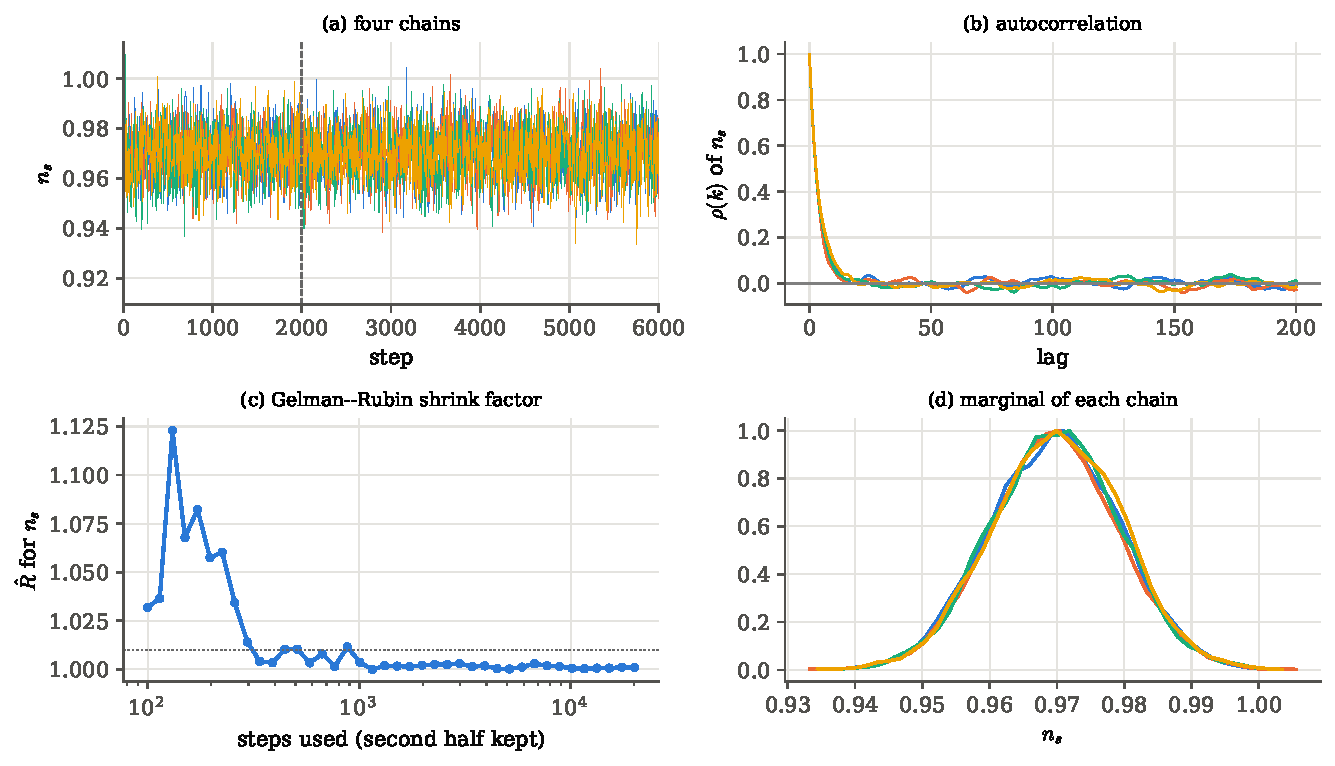
\includegraphics[width=0.9\linewidth]{figures/ch09/cmb_diag.pdf}
\caption{Diagnostics of the masked-sky chains, for $n_s$. (a) Traces of the four chains from dispersed starting
points; the dashed line marks the end of burn-in. (b) Autocorrelation functions after burn-in. (c) The
Gelman--Rubin $\hat R$ computed from the second half of the first $n$ steps, against $n$; the dotted line is
$1.01$. (d) The marginal of $n_s$ from each chain separately.}
\label{9c:fig:cmb-diag}
\end{figure}

\begin{center}
\small
\renewcommand{\arraystretch}{1.15}
\begin{tabular}{@{}lcccccc@{}}
\toprule
case & $\ln(10^{10}A_s)$ & $n_s$ & $\rho$ & Fisher $\sigma$'s, $\rho$ & acc., $\hat R$ & $\tau$, ESS\\\midrule
(a) sky & $\NineCToyFullA\pm\NineCToyFullSA$ & $\NineCToyFullN\pm\NineCToyFullSN$ & $\NineCToyFullRho$ & $\NineCToyFullFSA$, $\NineCToyFullFSN$, $\NineCToyFullFRho$ & $\NineCToyFullAcc$, $\NineCToyFullRhat$ & $\NineCToyFullTau$, $\NineCToyFullESS$\\
(b) noisy & $\NineCToyNoisyA\pm\NineCToyNoisySA$ & $\NineCToyNoisyN\pm\NineCToyNoisySN$ & $\NineCToyNoisyRho$ & $\NineCToyNoisyFSA$, $\NineCToyNoisyFSN$, $\NineCToyNoisyFRho$ & $\NineCToyNoisyAcc$, $\NineCToyNoisyRhat$ & $\NineCToyNoisyTau$, $\NineCToyNoisyESS$\\
(c) masked & $\NineCToyMaskA\pm\NineCToyMaskSA$ & $\NineCToyMaskN\pm\NineCToyMaskSN$ & $\NineCToyMaskRho$ & $\NineCToyMaskFSA$, $\NineCToyMaskFSN$, $\NineCToyMaskFRho$ & $\NineCToyMaskAcc$, $\NineCToyMaskRhat$ & $\NineCToyMaskTau$, $\NineCToyMaskESS$\\
truth & $\NineCToyTruthA$ & $\NineCToyTruthN$ & & & & \\
\bottomrule
\end{tabular}
\end{center}

The library cross-checks agree: \pyname{emcee} on the masked likelihood gives
$\ln(10^{10}A_s)=\NineCToyEmA\pm\NineCToyEmSA$ and $n_s=\NineCToyEmN\pm\NineCToyEmSN$, and \pyname{getdist}
\cite{Lewis2019GetDist}, the analysis package of CosmoMC and Cobaya, puts the 68 per cent interval of $n_s$ at
$[\NineCToyGdNlo,\NineCToyGdNhi]$, the same as our percentiles $[\NineCToyOurNlo,\NineCToyOurNhi]$.

\subsection{Reading the triangle plot}
\label{9c:sec:toy-triangle}

The standard display of a posterior with several parameters is the \newterm{triangle plot}
\unpack{one-dimensional marginals on the diagonal, two-dimensional marginals of each pair below it}. By the key
idea of \cref{9c:sec:line-marginal} every panel is a histogram of one or two columns of the chain. Ours is
written by hand in matplotlib (\pyname{triangle} in \pyname{lib_mcmc9c.py}) so that nothing is hidden, and two
choices in it need a word.

\emph{Where to draw the 68 per cent contour.} A two-dimensional histogram $H$ of the samples, smoothed slightly,
estimates the density on a grid. The 68 per cent region is the set of highest density holding 68 per cent of the
samples: sort the cells from the highest down, add up their contents until the total reaches 68 per cent, and the
height of the last cell added is the contour level.
\pyfile[firstline=107,lastline=112]{code/ch09/lib_mcmc9c.py}{The contour level that encloses a given probability}

\emph{Where to draw the Fisher ellipse.} For a two-dimensional Gaussian with covariance $\Cmat$, the quantity
$\Delta\chi^2=(\params-\bar\params)\T\Cmat^{-1}(\params-\bar\params)$ is a sum of two squared independent standard
Gaussians (rotate and rescale to the principal axes), so it follows $\chi^2_2$, whose cumulative distribution is
$1-e^{-c/2}$ (\cref{ch:02}). The ellipse $\Delta\chi^2=c$ encloses probability $p$ when
\[
  1-e^{-c/2}=p\quad\Longleftrightarrow\quad c=-2\ln(1-p):\qquad p=0.683\to c=2.30,\qquad p=0.954\to c=6.18 .
\]
In two dimensions the ``$1\sigma$'' ellipse is not $\Delta\chi^2=1$, which encloses only $1-e^{-1/2}=39$ per cent;
the one-dimensional $68.3$ per cent of $\pm1\sigma$ needs $\Delta\chi^2=2.30$ when two parameters are shown
together.

\Cref{9c:fig:cmb-triangle} shows the three posteriors with the Fisher ellipses of each case centred on the truth.

\begin{figure}[htbp]
\centering
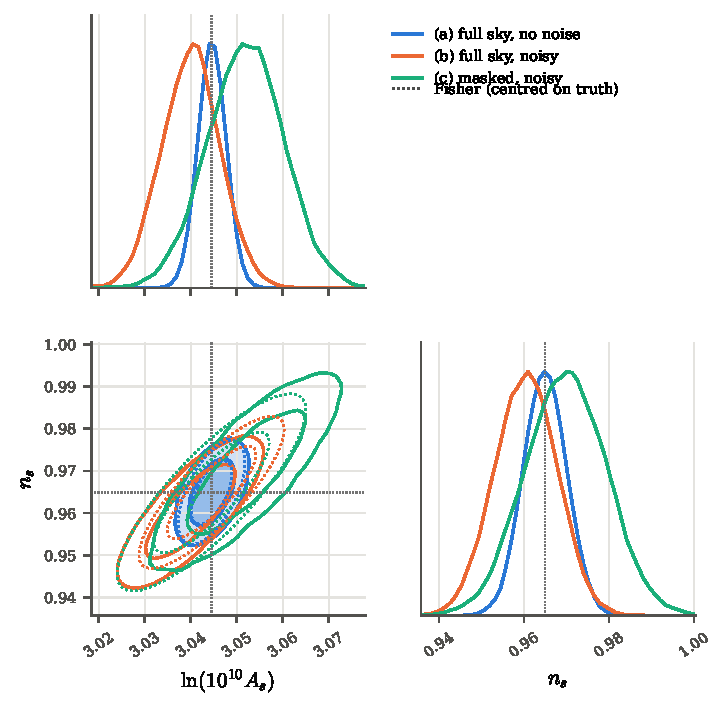
\includegraphics[width=0.66\linewidth]{figures/ch09/cmb_triangle.pdf}
\caption{Hand-made triangle plot of $(\ln10^{10}A_s,n_s)$ from one simulated sky observed three ways: the sky
itself (filled blue), the full sky with beam and noise (red), and the noisy sky behind the Galactic mask
(green). Diagonal: one-dimensional marginals. Lower panel: 68 and 95 per cent contours of the chains, with the
Fisher ellipses of each case centred on the truth (dotted) and the true values (dashed lines).}
\label{9c:fig:cmb-triangle}
\end{figure}

\subsection{Understanding the three posteriors}
\label{9c:sec:toy-understand}

\paragraph{The centres.} The three analyses see the same sky, so their centres are not independent draws; they
move only through what the noise adds and what the mask hides. Relative to their own widths, the noisy case sits
$\NineCToyNoisyPullA$ and $\NineCToyNoisyPullN$ standard deviations from the truth in $\ln(10^{10}A_s)$ and $n_s$,
the masked case $\NineCToyMaskPullA$ and $\NineCToyMaskPullN$: ordinary fluctuations.

\paragraph{The widths.} From the sky itself to the noisy sky the error of $\ln(10^{10}A_s)$ grows from
$\NineCToyFullSA$ to $\NineCToyNoisySA$, a factor of about two, and that of $n_s$ from $\NineCToyFullSN$ to
$\NineCToyNoisySN$, a factor of about one and a half. Where does the information go? The Fisher matrix
\eqref{9c:eq:fisher-cl} counts it multipole by multipole. With the beam divided out, so that $N_\ell$ is the
deconvolved noise power, each multipole enters with the weight
\[
  w_\ell=\frac\nu2\Bigl(\frac{\Cell}{\Cell+N_\ell}\Bigr)^2 ,
\]
which is the full-sky $\nu/2$ where the signal dominates and falls as $(\Cell/N_\ell)^2$ where the noise does. For our
experiment, $30'$ and $200\,\mu$K\,arcmin, the deconvolved noise $N_\ell=\Delta_T^2e^{\ell(\ell+1)\sigma_b^2}$
(\cref{9c:sec:emu-check}) is below a twentieth of the signal at $\ell=300$, equals it near $\ell\approx460$, and is
twelve times larger at $\ell=600$. Because the number of modes $2\ell+1$ grows with $\ell$, the multipoles above
the crossover carried much of the total: $\sum_\ell w_\ell$, which is the amplitude entry $F_{AA}$, keeps only 47 per
cent of its noiseless value. The tilt's entry $F_{nn}$ keeps 97 per cent, since it weights each multipole also by the
square of its lever arm in $\ln k$ (next paragraph), which is largest at the low multipoles the noise does not touch.
The tilt's error still grows, through the correlation: with the high multipoles gone, amplitude and tilt can trade
more freely. These weights reproduce the chains' widths to about ten per cent; the remainder comes from the pixel window
and the other details of the simulation that this count leaves out.

The mask then removes a third of the sky. On a fraction $\fsky$ of the sky each multipole has about $(2\ell+1)\fsky$
independent modes instead of $2\ell+1$ (Knox's mode count, \cref{8a:sec:knox}), so every $w_\ell$, and with them the
whole Fisher matrix, is multiplied by $\fsky$, and every error by $1/\sqrt{\fsky}=1/\sqrt{\NineCToyFsky}\approx1.23$. The
chains give $\NineCToyMaskSA/\NineCToyNoisySA\approx1.32$ for both parameters. The extra seven per cent is the taper:
pixels near the mask edge are kept with weights below one, so they carry less than their share of modes.

In every case the chain and the Fisher matrix agree to the second decimal. That follows from two facts already
shown. By \eqref{9c:eq:dlnC} the parameters enter $\ln\Cell$ almost linearly, and a likelihood that is quadratic in a
quantity linear in the parameters is a Gaussian in the parameters, as for the straight line; and with hundreds of
multipoles each term of the sum is close to its quadratic expansion \eqref{9c:eq:dchi2}. So the posterior is nearly
Gaussian, and its covariance is the inverse Fisher matrix.

\paragraph{The correlation: a straight line in disguise.} Why is the correlation $+\NineCToyFullRho$, and why does it
grow to $+\NineCToyNoisyRho$ with noise? Give a name to the derivative of \eqref{9c:eq:dlnC}: for each multipole let
\[
  s_\ell\equiv\frac{\partial\ln\Cell}{\partial n_s}=\langle\ln(k/k_*)\rangle_\ell ,
\]
the average distance in $\ln k$ from the pivot of the wavenumbers that feed multipole $\ell$ (in \cref{9c:sec:emu-log}
the integration variable $\ln(k/k_*)$ was called $x$; $s_\ell$ is its average, one number per multipole). Near the
fiducial model, to first order,
\[
  \ln\Cell(\params)\simeq\ln\Cell(\params_0)+\delta\ln A_s+s_\ell\,\delta n_s,
\]
a straight line in the variable $s_\ell$, with intercept $\delta\ln A_s$ and slope $\delta n_s$. Its Fisher matrix
follows from \eqref{9c:eq:fisher-cl} in two lines:
\begin{align}
  \partial_i\Cell\,\partial_j\Cell
  &\eqby{1}\Cell^2\,\frac{\partial\ln\Cell}{\partial\theta_i}\frac{\partial\ln\Cell}{\partial\theta_j}
   \eqby{2}\Cell^2\begin{pmatrix}1&s_\ell\\s_\ell&s_\ell^2\end{pmatrix}_{ij},
  \qquad
  F\eqby{3}\sum_\ell w_\ell\begin{pmatrix}1&s_\ell\\s_\ell&s_\ell^2\end{pmatrix}.
  \label{9c:eq:toy-fisher}
\end{align}
\begin{explain}
  \item $\partial\Cell=\Cell\,\partial\ln\Cell$.
  \item $\partial\ln\Cell/\partial\ln A_s=1$ and $\partial\ln\Cell/\partial n_s=s_\ell$, from the line above.
  \item Put this into \eqref{9c:eq:fisher-cl}: $\frac\nu2\Cell^2/(\Cell+N_\ell)^2$ is the weight $w_\ell$ of the previous
        paragraph.
\end{explain}
This is exactly the matrix of the straight-line fit \eqref{9c:eq:line-2x2}, with $s_\ell$ in place of $x_i$ and $w_\ell$ in
place of $1/\sigma_i^2$. So the result of \cref{9c:sec:line-exact} applies unchanged:
\[
  \rho(\ln A_s,n_s)=-\frac{\bar s_w}{\sqrt{\overline{s^2}_w}} ,
\]
with $\bar s_w$ and $\overline{s^2}_w$ the $w$-weighted means of $s_\ell$ and $s_\ell^2$. The pivot $k_*=0.05$\,Mpc$^{-1}$ is
the origin $s=0$ of this line, and it falls at a multipole of a few hundred (\cref{9c:sec:emu-log}). Our data stop at
$\ell=601$ and most of their weight is at lower multipoles, where $s_\ell<0$: the weighted mean is negative and the
correlation positive. Noise removes the high multipoles, nearest the pivot, so $\bar s_w$ moves further from zero and
the correlation grows. A Planck-like experiment measures out to $\ell=2500$, where $s_\ell>0$, and the sign flips
(\cref{9c:sec:planck}). Choosing the pivot is choosing the origin of $s$, Kruschke's centring of
\cref{9c:sec:line-centre} in cosmological dress: a pivot at the weighted centre of the data would make amplitude and
tilt uncorrelated.

\subsection{Do the Gaussian approximations bias \texorpdfstring{$n_s$}{n\_s}?}
\label{9c:sec:toy-gauss}

On the noiseless full sky we know the exact likelihood, so we can test the approximations of
\cref{9c:sec:cl-approx} on parameters. Running the chain with $\Like_Q$ (variance from the model) and with $\Like_f$
(variance from the fixed fiducial) instead of the exact form, on the same sky, gives the posteriors of
\cref{9c:fig:cmb-gauss}a: $\Like_f$ coincides with the exact one, while $\Like_Q$ moves $n_s$ by $\NineCToyShiftQ$
standard deviations. One sky could be a fluke, so we repeat the comparison of best fits on $\NineCToyEnsN$
skies drawn from the exact $\chi^2$ distribution. Relative to the exact best fit, $\Like_Q$ shifts $n_s$ by
$\NineCToyEnsQmean\pm\NineCToyEnsQsd$ standard deviations (mean and scatter over skies) and $\ln(10^{10}A_s)$ by
$\NineCToyEnsQAmean$; $\Like_f$ shifts $n_s$ by $\NineCToyEnsFmean\pm\NineCToyEnsFsd$ (\cref{9c:fig:cmb-gauss}b). This
is HL's statement, ``$\Like_Q$ biases parameters like the spectral index by around one sigma, $\Like_f$ is unbiased''
\cite{HamimecheLewis2008}, reproduced on our experiment. The mechanism is the $0.9/\ell$ upward bias of the spectrum
derived in \eqref{9c:eq:AQ-bias}: largest at low $\ell$, so it is read as extra power on large scales, a lower
$n_s$ and a slightly higher amplitude.

The same $\NineCToyEnsN$ skies give a check of the exact analysis itself. Its best-fit $n_s$ scatters about the
truth with mean $\NineCToyEnsExactBias$ and standard deviation $\NineCToyEnsExactSd$ in units of the Fisher error:
unbiased, and with error bars that mean what they say, to the precision of 500 skies (about $\pm0.03$ on the
standard deviation).

\begin{figure}[htbp]
\centering
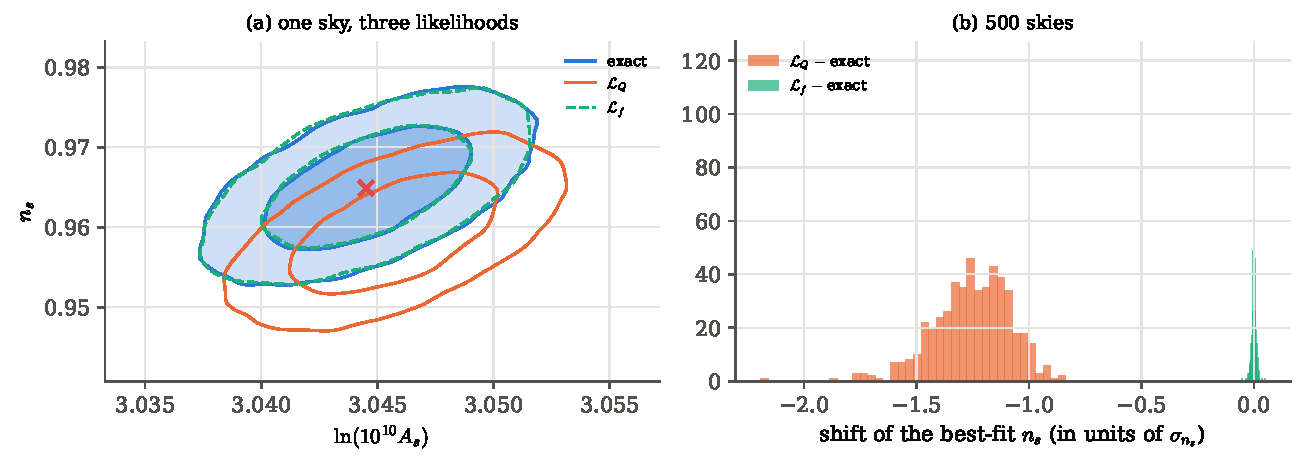
\includegraphics[width=0.9\linewidth]{figures/ch09/cmb_gauss_bias.pdf}
\caption{Gaussian approximations on the noiseless full sky. (a) One sky, three likelihoods: exact (filled),
$\Like_Q$ and $\Like_f$; $\Like_f$ lies on the exact contours, $\Like_Q$ is displaced to lower $n_s$. (b) Over 500 skies, the
shift of the best-fit $n_s$ from its exact value, in units of the expected error: $\Like_Q$ is off by more than one
standard deviation in every sky, $\Like_f$ by less than a hundredth.}
\label{9c:fig:cmb-gauss}
\end{figure}
\section{Reproducing Planck 2018: the amplitude and tilt of the primordial spectrum}
\label{9c:sec:planck}

How did the fluctuations that grew into galaxies start out? The simplest models of the early Universe predict a
primordial spectrum that is almost a power law, $P(k)=A_s(k/k_*)^{n_s-1}$, described by two numbers: its amplitude
$A_s$ at the pivot wavenumber $k_*=0.05$\,Mpc$^{-1}$ and its tilt $n_s$ (\cref{8a:sec:lit-pivot}). A tilt of exactly one
would mean the same strength of fluctuations on every scale; a tilt slightly below one, more on large scales, is
what the simplest models of inflation predict. A CMB temperature map is the cleanest view of that spectrum we
have: the sky is one realisation of $\Cell(\params)$, and the spectrum is a weighted integral of $P(k)$
(\cref{9c:sec:emu-log}).

\paragraph{The question.} How well does Planck's temperature map, with its low-multipole polarization, measure the
amplitude and the tilt, and how much of the answer depends on which other parameters are left free? We cannot
reproduce Planck's centres: they belong to the one real sky. We can reproduce the widths and the correlation,
which depend on the experiment and on the model, not on the sky, and we can trace every difference to a cause.

\subsection{Planck's setup and likelihood}
\label{9c:sec:planck-their}

\emph{The maps.} Planck's high-$\ell$ temperature likelihood uses three frequency channels, 100, 143 and 217\,GHz,
each observed in two halves of the mission. Spectra are formed only between different halves, so the noise of one
half is uncorrelated with the other and adds no power on average (\cref{9c:sec:pipeline}).

\emph{The masks.} Each channel has its own mask, removing the Galactic plane and point sources, and leaving a
different fraction of the sky, because dust emission grows with frequency \cite{Planck2018V}.

\emph{The foregrounds and the instrument.} What remains on the sky is not only the CMB. Planck describes dust,
point sources, the thermal and kinetic Sunyaev--Zeldovich effects, the cosmic infrared background and the relative
calibrations of the channels with about fifteen nuisance parameters, sampled alongside the six cosmological ones.

\emph{The low multipoles.} Below $\ell=30$, the Blackwell--Rao likelihood of \cref{9c:sec:hl} for temperature, and the
lowE polarization likelihood, which measures the optical depth $\tau=0.0506\pm0.0086$ on its own \cite{Planck2018VI}.
\begin{center}
\small
\renewcommand{\arraystretch}{1.15}
\begin{tabular}{@{}lccc@{}}
\toprule
channel & 100\,GHz & 143\,GHz & 217\,GHz\\\midrule
sky fraction of the temperature mask & $0.66$ & $0.57$ & $0.47$\\
\bottomrule
\end{tabular}
\qquad
\begin{tabular}{@{}ll@{}}
\toprule
range & likelihood\\\midrule
$2\le\ell<30$ & Blackwell--Rao; lowE for $\tau$\\
$\ell\ge30$ & Gaussian, fiducial covariance\\
\bottomrule
\end{tabular}
\end{center}

\paragraph{Their key equation.} Above $\ell=30$ Planck's likelihood is a Gaussian in the vector $\widehat{\bm C}$ of all
the binned cross-spectra, with a covariance $\bm\Sigma$ computed once for a fiducial model (Planck 2018 V, eq.~20):
$-2\ln\Like=(\widehat{\bm C}-\bm C(\params))\T\bm\Sigma^{-1}(\widehat{\bm C}-\bm C(\params))+\text{const}$, where $\bm C(\params)$
holds the cosmological spectrum plus the foreground model, scaled by the calibrations. The symbol map to our
notation is short. Their $\widehat{\bm C}$ is our $\Chat$ for one channel and no binning; their $\bm C(\params)$ is our
$\Cell(\params)$ plus the noise power $N_\ell$ (we use one map, whose spectrum contains its noise, where Planck uses
cross-spectra without it) and with no foregrounds; their $\bm\Sigma$ is diagonal for us, with the $\fsky$ mode count of
\cref{9c:sec:cl-exact}. Then
\begin{align}
  -2\ln\Like
  &\eqby{1}\sum_\ell\frac{\bigl(\Chat-\Cell(\params)-N_\ell\bigr)^2}{\Sigma_{\ell\ell}}
   \eqby{2}\sum_\ell\frac{(2\ell+1)\fsky}{2}\Bigl[\frac{\Chat-\Cell(\params)-N_\ell}{C^{\rm f}_\ell+N_\ell}\Bigr]^2 .
  \label{9c:eq:planck-gauss-ours}
\end{align}
\begin{explain}
  \item One channel, one spectrum per multipole, and no coupling between multipoles: $\bm\Sigma$ is diagonal.
  \item The variance of $\Chat$ is $2(\Cell+N_\ell)^2/\nu$ with $\nu=(2\ell+1)\fsky$ (\cref{9c:sec:cl-approx}), evaluated
        once at the fiducial spectrum $C^{\rm f}_\ell$.
\end{explain}
This is the fixed-fiducial $\Like_f$ of \cref{9c:sec:cl-approx}, with the noise added. On our idealised data the exact
form is available, so our runs use it, and \cref{9c:sec:planck-gauss} measures what replacing it by
\eqref{9c:eq:planck-gauss-ours} costs. What we drop, then, is the second and third channels, the mode coupling of a
real mask, and all the foreground and calibration parameters.

\paragraph{The numbers to reproduce.} With this likelihood, temperature plus lowE gives
$\ln(10^{10}A_s)=3.040\pm0.016$ and $n_s=0.9626\pm0.0057$ (Planck 2018 VI, Table~2, column TT+lowE
\cite{Planck2018VI}). The covariance matrix that the Planck team distributes with its chains adds the correlation
between the two, $\NineCPlPubRho$, with widths $\NineCPlPubCovSA$ and $\NineCPlPubCovSN$.

\subsection{The simulated experiment and its likelihood}
\label{9c:sec:planck-setup}

\emph{The spectrum.} The true spectrum is computed by CAMB at the fiducial parameters (not by the emulator, so
the emulator's error is part of the test). The noise is that of the 143\,GHz channel, $7.22'$ and
$33\,\mu$K\,arcmin \cite{Planck2018I}, and the sky fraction is $\fsky=\NineCPlFsky$, the fraction left by Planck's
143\,GHz temperature mask \cite{Planck2018V}. The measured spectrum is drawn as
$\Chat=(\Cell+N_\ell)\,\chi^2_\nu/\nu$ with $\nu=(2\ell+1)\fsky$ at every $2\le\ell\le\NineCPlLmax$: the
distribution of \cref{9c:sec:cl-exact} with the mode count of a partial sky.

\emph{The likelihood.} For these data the $\fsky$-scaled exact form is the true likelihood,
\begin{equation}
  -2\ln\Like(\params)=\sum_{\ell=2}^{2500}(2\ell+1)\fsky\Bigl[\frac{\Chat}{\Cell(\params)+N_\ell}+\ln\bigl(\Cell(\params)+N_\ell\bigr)\Bigr]
  +\frac{(\tau-\tau_{\rm obs})^2}{\sigma_\tau^2}.
  \label{9c:eq:planck-like}
\end{equation}
The last term stands in for Planck's low-$\ell$ polarization likelihood (lowE), which on its own measures
$\tau=0.0506\pm0.0086$ \cite{Planck2018VI}. We simulate that measurement too: $\tau_{\rm obs}$ is drawn from a
Gaussian of width $\sigma_\tau=\NineCPlSigTau$ about the true $\tau=\NineCPlTauTrue$, and the draw gave
$\tau_{\rm obs}=\NineCPlTauObs$, two standard deviations high. In code:
\pyfile[firstline=59,lastline=75]{code/ch09/45_planck_like.py}{The Planck-like log posterior}

\emph{Three runs}, each asking a different question:
\begin{itemize}[itemsep=1pt]
  \item P2: \emph{if we knew everything else}, how well would the spectrum fix the amplitude and the tilt? Only
        $(\ln10^{10}A_s,n_s)$ are free; $H_0$, $\omega_b$, $\omega_c$ and the optical depth $\tau$ are fixed at the truth.
  \item P3: what changes when the reionisation optical depth $\tau$ is left free, constrained only by its lowE prior?
  \item P6: the full problem, with all six $\Lambda$CDM parameters free.
\end{itemize}
Every run has $\NineCPlNch$ chains of $\NineCPlNst$ steps, a proposal shaped by the Fisher covariance, and $\NineCPlBurn$
steps of burn-in. The diagnostics of \cref{9b:sec:diagnostics} are below; to keep $\tau$ for the optical depth, the
integrated autocorrelation time (written $\tau$ in \cref{9c:sec:line-chain}) is called $t_{\rm ac}$ here.
\begin{center}
\small
\renewcommand{\arraystretch}{1.15}
\begin{tabular}{@{}lcccccc@{}}
\toprule
run & free & emulator & time (s) & acceptance & largest $\hat R$ & $t_{\rm ac}$ (steps)\\\midrule
P2 & $\ln10^{10}A_s,n_s$ & first order & $\NineCPlTwoSec$ & $\NineCPlTwoAcc$ & $\NineCPlTwoRhat$ & $\NineCPlTwoTau$\\
P3 & $+\tau$ & first order & $\NineCPlThreeSec$ & $\NineCPlThreeAcc$ & $\NineCPlThreeRhat$ & $\NineCPlThreeTau$\\
P6 & all six & second order & $\NineCPlSixSec$ & $\NineCPlSixAcc$ & $\NineCPlSixRhat$ & up to $\NineCPlSixTau$\\
\bottomrule
\end{tabular}
\end{center}
All three chains can be trusted. Their widths, against Planck's:
\begin{center}
\small
\renewcommand{\arraystretch}{1.15}
\begin{tabular}{@{}lccc@{}}
\toprule
 & $\sigma(\ln10^{10}A_s)$ & $\sigma(n_s)$ & $\rho(\ln A_s,n_s)$\\\midrule
Planck 2018 TT+lowE, Table 2 & $0.016$ & $0.0057$ & \\
Planck chains' covariance & $\NineCPlPubCovSA$ & $\NineCPlPubCovSN$ & $\NineCPlPubRho$\\\midrule
P2: 2 free, others fixed & $\NineCPlTwoSA$ & $\NineCPlTwoSN$ & $\NineCPlTwoRho$\\
\quad Fisher & $\NineCPlTwoFSA$ & $\NineCPlTwoFSN$ & $\NineCPlTwoFRho$\\
P3: $+\tau$, lowE prior & $\NineCPlThreeSA$ & $\NineCPlThreeSN$ & $\NineCPlThreeRho$\\
\quad Fisher & $\NineCPlThreeFSA$ & $\NineCPlThreeFSN$ & $\NineCPlThreeFRho$\\
P6: all 6 free & $\NineCPlSixSA$ & $\NineCPlSixSN$ & $\NineCPlSixRho$\\
\quad Fisher & $\NineCPlSixFSA$ & $\NineCPlSixFSN$ & $\NineCPlSixFRho$\\\midrule
ratio P6 / Planck & $\NineCPlRatioSA$ & $\NineCPlRatioSN$ & \\
\bottomrule
\end{tabular}
\end{center}

With all six parameters free we recover Planck's widths to within ten per cent. Reading down the table, freeing $\tau$
(P2 to P3) multiplies the amplitude's error by nine and leaves the tilt's alone; freeing the other three (P3 to P6)
doubles the tilt's error and leaves the amplitude's alone. The next two subsections explain each step, and the
third the correlation (\cref{9c:fig:planck-triangle}).

\begin{figure}[htbp]
\centering
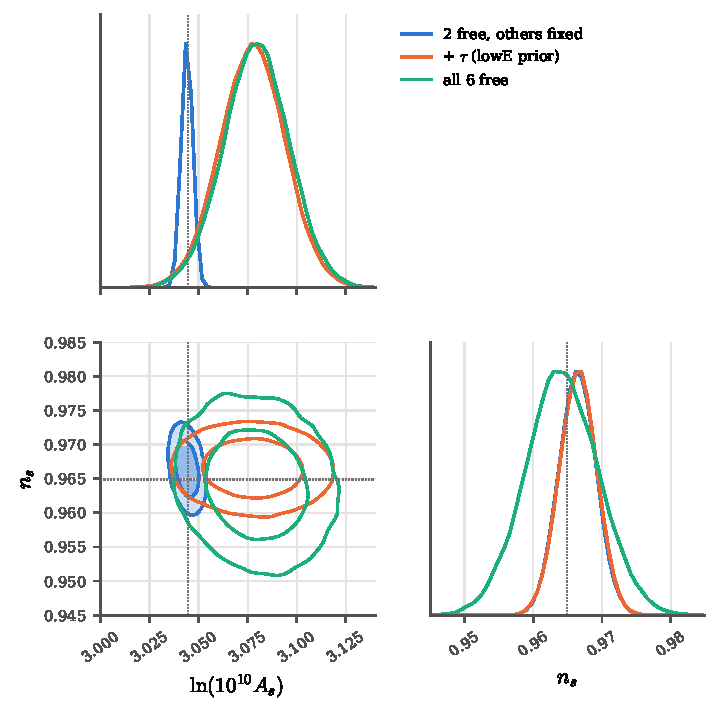
\includegraphics[width=0.66\linewidth]{figures/ch09/planck_triangle.pdf}
\caption{$(\ln10^{10}A_s,n_s)$ from the Planck-like simulated spectrum, with two parameters free and the rest fixed
(filled blue), with $\tau$ free under the lowE prior (red), and with all six $\Lambda$CDM parameters free (green).
Dashed lines: the true values. Freeing $\tau$ stretches the amplitude ninefold; freeing $H_0$, $\omega_b$ and
$\omega_c$ doubles the tilt's error and removes most of the correlation.}
\label{9c:fig:planck-triangle}
\end{figure}

\subsection{Why the amplitude needs \texorpdfstring{$\tau$}{tau}}
\label{9c:sec:planck-tau}

Above $\ell\approx30$ the temperature spectrum depends on $A_s$ and $\tau$ only through $A_se^{-2\tau}$
(\cref{9c:sec:emu-log}), that is, through the combination $c=\ln(10^{10}A_s)-2\tau$. A temperature spectrum measures
$c$ precisely and says almost nothing about $\ln A_s$ and $\tau$ separately (the opposite flat responses in
\cref{9c:fig:emu-derivs}). In P3 the chain's column of $\ln(10^{10}A_s)-2\tau$ has standard deviation
$\NineCPlSdComb$, the same as $\sigma(\ln A_s)$ in P2, where $\tau$ was fixed and the whole of $c$ was attributed to
$A_s$. The amplitude itself is then pinned only by lowE. Write $\ln(10^{10}A_s)=c+2\tau$. Are $c$ and $\tau$
independent? Change variables from $(\ln10^{10}A_s,n_s,\tau)$ to $(c,n_s,\tau)$, a shift with unit Jacobian, so flat
priors stay flat. Above $\ell=30$ the TT term of \eqref{9c:eq:planck-like} depends on the amplitude and the optical
depth only through $c$; the lowE term depends only on $\tau$. The likelihood is then a function of $(c,n_s)$ times a
function of $\tau$, and with flat priors so is the posterior: $c$ and $\tau$ are independent, up to the weak
information TT has on $\tau$ below $\ell=30$. The chain agrees: the correlation of its $c$ and $\tau$ columns in P3 is
$-0.05$. So
\begin{align}
  \sigma^2(\ln10^{10}A_s)
  &\eqby{1}\sigma_c^2+4\sigma_\tau^2
   \eqby{2}\NineCPlSdComb^2+4\times\NineCPlThreeST^2
   \quad\Rightarrow\quad\sigma(\ln10^{10}A_s)\approx0.0165,
  \nonumber\\
  \rho(\ln A_s,\tau)&\eqby{3}\frac{2\sigma_\tau^2}{\sigma(\ln A_s)\,\sigma_\tau}\approx0.99 .
  \label{9c:eq:As-tau}
\end{align}
\begin{explain}
  \item The variance of a sum of independent quantities, with the factor 2 squared.
  \item $\sigma_c=\NineCPlSdComb$ from the chain; $\sigma_\tau=\NineCPlThreeST$, the posterior width of $\tau$, which
        is the lowE width slightly narrowed by the weak information TT has on $\tau$ at $\ell<30$.
  \item $\Cov(c+2\tau,\tau)=2\sigma_\tau^2$.
\end{explain}
The chain gives $\NineCPlThreeSA$ and $\NineCPlThreeRhoAT$. The published $0.016$ is the same calculation with
Planck's $\sigma_\tau=0.0080$: our width is larger by about the ratio of the two $\tau$ errors, $\NineCPlThreeST/0.0080\approx1.03$,
which is the origin of the $\NineCPlRatioSA$ of the table. The amplitude of the primordial spectrum, as measured by the CMB, is
a measurement of the optical depth to reionisation.

\paragraph{Example: why our amplitude is high.} Our six-parameter chain centres on
$\ln(10^{10}A_s)=\NineCPlSixMA$, while the truth is $\NineCPlTruthA$: a shift of two standard deviations. By the same
argument it must follow the simulated lowE measurement, which came out high by $\tau_{\rm obs}-\tau_{\rm true}=0.0714-0.0544=0.017$;
the posterior of $\tau$ is $\NineCPlSixMT$, and $2\times(0.0705-0.0544)=0.032$ is the shift of $\ln A_s$. A two-sigma
fluctuation of one external measurement moved the amplitude by two sigma, and TT could not object, because TT
fixes only $c$.

\subsection{Why the tilt needs the other parameters}
\label{9c:sec:planck-ns}

With $\omega_b$, $\omega_c$ and $H_0$ fixed (P3), $\sigma(n_s)=\NineCPlThreeSN$; with them free (P6), $\NineCPlSixSN$, a factor
$\NineCPlGainN$. How
much a parameter's error grows when others are freed can be read from the Fisher matrix
\eqref{9c:eq:fisher-cl}. Split the parameters into $n_s$ and the rest, $r$. The inverse of a matrix split this way has
the Schur-complement form already used in \eqref{8b:eq:schur}:
\begin{align}
  \sigma^2(n_s)
  &\eqby{1}(\Fish^{-1})_{nn}
   \eqby{2}\frac{1}{F_{nn}-\bm F_{nr}\Fish_{rr}^{-1}\bm F_{rn}}
   \eqby{3}\frac{1}{F_{nn}\,(1-R^2)},
  \qquad R^2\equiv\frac{\bm F_{nr}\Fish_{rr}^{-1}\bm F_{rn}}{F_{nn}} .
  \label{9c:eq:ns-R2}
\end{align}
\begin{explain}
  \item The marginal error, with all the other free parameters integrated out (\cref{9c:sec:emu-check}).
  \item Block inversion: the $(n,n)$ element of the inverse is one over the Schur complement of $\Fish_{rr}$.
  \item Factor out $F_{nn}$; $1/\sqrt{F_{nn}}$ is the error with everything else fixed.
\end{explain}
$R^2$ is a number between zero and one: the fraction of the effect of $n_s$ on the spectrum, measured in the Fisher
metric, that some combination of the other parameters can reproduce (the multiple correlation of the derivative
curves of \cref{9c:fig:emu-derivs}). For our experiment $1/\sqrt{F_{nn}}=0.0018$. With $\ln A_s$ and $\tau$ free,
$R^2=0.53$ and $\sigma(n_s)=0.0018/\sqrt{0.47}=0.0026$; with all five free, $R^2=0.89$ and
$\sigma(n_s)=0.0018/\sqrt{0.11}=0.0053$, the chains' values. A doubling of the error is a factor of four in $1-R^2$:
of the part of $n_s$'s effect that amplitude and optical depth cannot mimic, $H_0$, $\omega_b$ and $\omega_c$ together
mimic three quarters.

Which of them? Freed one at a time (with $\ln A_s$ and $\tau$), each moves $\sigma(n_s)$ by less than four per cent:
$0.0027$ for $H_0$ or $\omega_b$, $0.0026$ for $\omega_c$. Freed together, $H_0$ and $\omega_c$ give $0.0049$, and adding
$\omega_b$ completes the $0.0053$. The physical reading follows from these numbers. Changing $H_0$ or $\omega_c$ alone
moves the acoustic peaks sideways in $\ell$, which the spectrum measures far too well to allow; changing both together,
in the proportion that keeps the angular size of the sound horizon fixed, leaves the peaks in place and changes the
matter density, which alters the driving of the oscillations and so the heights of the first peaks relative to the
later ones. A change of relative heights across $\ell$ is what a tilt does, so $n_s$ becomes partly degenerate with that
combination; the baryon density, which raises the odd peaks against the even ones, takes a smaller share.
This is the pitfall of \cref{9c:sec:exp-sigma} on a
cosmological scale: a nuisance parameter fixed at its true value hides an uncertainty, and the chain cannot tell.
The remaining seven per cent between our $\NineCPlSixSN$ and Planck's $0.0057$ is what we left out
(\cref{9c:sec:planck-their}): the fifteen foreground and calibration parameters that Planck's official TT chains
sample alongside the six (they are listed in the covariance file we used), and three frequency channels with
different noise, beams and masks \cite{Planck2018V}. By \eqref{9c:eq:ns-R2}, each nuisance parameter that can mimic part of the effect of $n_s$ at high $\ell$ widens it a little.
Our one clean channel with no foregrounds is slightly too optimistic.

The other widths tell the same story (\cref{9c:fig:planck-overlay}b): $H_0$ to $\pm\NineCPlSixSH$ against Planck's $0.92$,
$\omega_b$ to $\NineCPlSixSB$ against $0.00022$, $\omega_c$ to $\NineCPlSixSC$ against $0.0021$, $\tau$ to $\NineCPlSixST$
against $0.0080$, all within about ten per cent.\footnote{Planck samples $100\,\theta_{\rm MC}$, the angular size of the
sound horizon, where we sample $H_0$. The marginal of $(\ln A_s,n_s)$ does not care how the integrated-out parameters
are labelled: a change of variables $\phi\to\psi(\phi)$ inside $\int p(\params,\phi)\,\dd\phi$ only multiplies the prior
by the Jacobian $\abs{\dd\phi/\dd\psi}$, so flat priors in different bases differ slightly, and with Planck's data the
likelihood dominates.}

\subsection{The correlation, and why the pivot is at \texorpdfstring{$0.05\,$Mpc$^{-1}$}{0.05/Mpc}}
\label{9c:sec:planck-pivot}

With the other parameters fixed the correlation is strongly negative, $\NineCPlTwoRho$, the opposite sign to the toy
experiment of \cref{9c:sec:toy-understand}, and the straight-line formula
$\rho=-\bar s_w/\sqrt{\overline{s^2}_w}$ of that section explains the sign. Planck's information extends to
$\ell\approx2000$, beyond the multipole of a few hundred that sees the pivot, so the weighted mean of
$s_\ell=\langle\ln(k/k_*)\rangle_\ell$, the lever arm of multipole $\ell$ in $\ln k$, is positive and $\rho<0$; the toy
stopped at $\ell=601$, where $s_\ell<0$, and had $\rho>0$. With $\tau$ free the correlation drops to $\NineCPlThreeRho$,
with all six free to $\NineCPlSixRho$ (Fisher $\NineCPlSixFRho$), and Planck finds $\NineCPlPubRho$. Why does it nearly
vanish?

\emph{Moving the pivot.} \Cref{8a:sec:lit-pivot} answered this with two lines. The same spectrum read at another
wavenumber $k'$, a distance $L=\ln(k'/k_*)$ away in $\ln k$, has amplitude
$\ln A(k')=\ln A_s+(n_s-1)L$, by $P(k)=A_s(k/k_*)^{n_s-1}$; its covariance with the tilt is
\begin{equation}
  \Cov\bigl(\ln A(k'),n_s\bigr)=\Cov(\ln A_s,n_s)+L\,\Var(n_s),
\end{equation}
zero at $L_{\rm dec}=-\Cov(\ln A_s,n_s)/\Var(n_s)$ \eqref{8a:eq:kdec}. Dividing by the two widths, the correlation at
the pivot itself is
\begin{equation}
  \rho(\ln A_s,n_s)=\frac{\Cov(\ln A_s,n_s)}{\sigma(\ln A_s)\,\sigma(n_s)}=-L_{\rm dec}\,\frac{\sigma(n_s)}{\sigma(\ln A_s)} .
  \label{9c:eq:rho-Ldec}
\end{equation}
So the correlation at $k_*$ is small if the decorrelation wavenumber is close to $k_*$, \emph{or} if the amplitude's
error is large compared with $L_{\rm dec}$ times the tilt's.

\emph{The numbers from our chains.} In P2, $\sigma(\ln A_s)=\NineCPlTwoSA$, $\sigma(n_s)=\NineCPlTwoSN$ and
$\rho=\NineCPlTwoRho$ give $L_{\rm dec}=0.50$, so $k_{\rm dec}=0.05\,e^{0.50}=0.082$\,Mpc$^{-1}$, the value
\cref{8a:sec:lit-pivot} found for a Planck-like experiment by Fisher matrix. In P6, $L_{\rm dec}=0.43$ and
$k_{\rm dec}=0.077$\,Mpc$^{-1}$: freeing the other parameters hardly moves the decorrelation scale. What changes is the
ratio in \eqref{9c:eq:rho-Ldec}: $\NineCPlTwoSN/\NineCPlTwoSA=1.5$ in P2 but $\NineCPlSixSN/\NineCPlSixSA=0.32$ in P6, so
$\rho=-0.50\times1.5=-0.73$ becomes $-0.43\times0.32=-0.14$. The drop is the factor of nine in the amplitude's error of
\cref{9c:sec:planck-tau}: the optical depth adds the same uncertainty $2\sigma_\tau$ to $\ln A$ at every pivot, and that
common part is uncorrelated with the tilt. This is also why P3, with only $\tau$ freed, already has
$\rho=\NineCPlThreeRho$. Planck's own $+0.03$ corresponds to $L_{\rm dec}=-0.03\times0.0164/0.0057\approx-0.09$, a
$k_{\rm dec}$ near $0.046$\,Mpc$^{-1}$; their extra nuisance parameters, which absorb high-$\ell$ power, plausibly move the
weighted centre of the tilt's information to lower $\ell$, but with $\rho$ this small the difference is within what the
two analyses' different ingredients can produce.

\emph{A pivot far away.} The same formula prices the alternative. At WMAP's pivot, $k'=0.002$\,Mpc$^{-1}$,
$L=\ln(0.002/0.05)=-3.2$, and our P6 chain gives $\rho\bigl(\ln A(k'),n_s\bigr)=-0.76$ with
$\sigma\bigl(\ln A(k')\bigr)=0.025$, half as large again as at $k_*$; in P2 the correlation there is $-0.99$. By the
centring argument of \cref{9c:sec:line-centre}, the amplitude read far from the data's weighted centre swings with every
error in the slope.

That is the reason for the convention. The pivot $k_*=0.05$\,Mpc$^{-1}$ defines what $A_s$ means, the amplitude of the
primordial spectrum at that wavenumber. Any other choice describes the same spectrum, but a pivot near the centre of
the data's information, within a factor of two of $k_{\rm dec}$ in either direction, makes the amplitude and the tilt
nearly independent, which makes them easier to quote, to combine and to sample.

\begin{figure}[htbp]
\centering
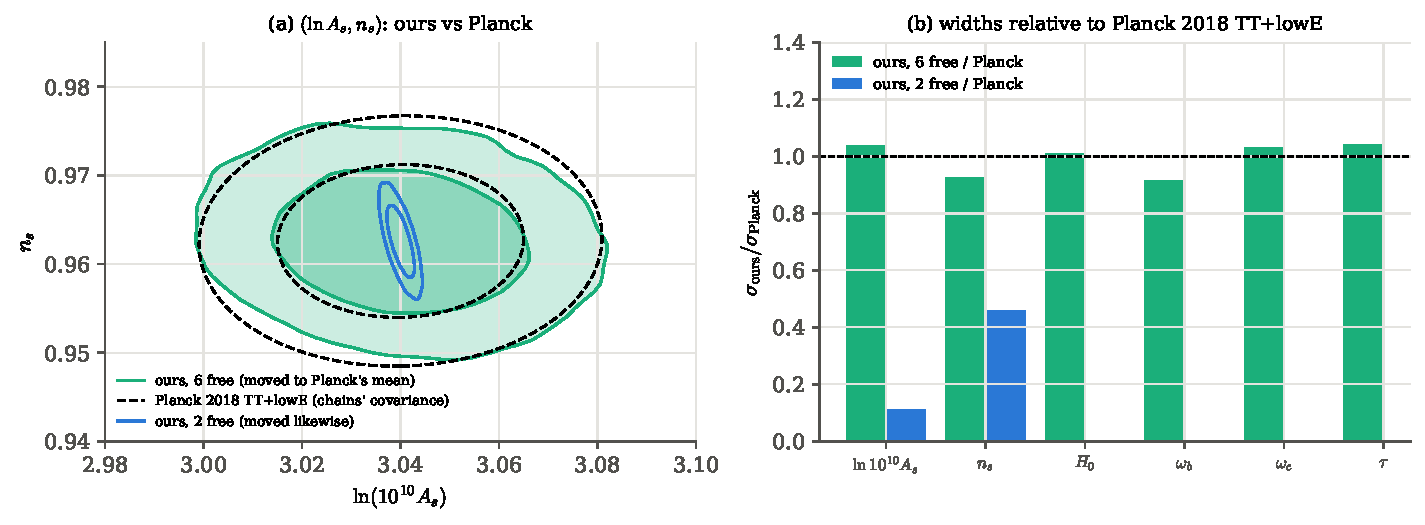
\includegraphics[width=\linewidth]{figures/ch09/planck_overlay.pdf}
\caption{Ours against Planck 2018 TT+lowE. (a) The 68 and 95 per cent contours of our six-parameter run (filled
green) and two-parameter run (blue), both shifted to Planck's centre since the centres belong to different skies,
with the Gaussian of the official chains' covariance (black dashed). (b) Posterior widths of all six parameters
divided by Planck's: with everything free (green) they are within about ten per cent; fixing the other four (blue)
makes $\ln A_s$ nine times and $n_s$ twice too precise.}
\label{9c:fig:planck-overlay}
\end{figure}

\subsection{Planck's Gaussian approximation, tested}
\label{9c:sec:planck-gauss}

Planck's high-$\ell$ likelihood is a Gaussian with a fiducial covariance (\cref{9c:sec:hl}), with the remark that its
symmetric shape biases $n_s$ by about $0.1\sigma$ \cite{Planck2018V}. In our setting we can measure the effect of that
choice, because we know the exact likelihood. For $\NineCPlBiasN$ simulated Planck-like spectra we find the best-fit
$(\ln A_s,n_s)$ under the exact likelihood \eqref{9c:eq:planck-like} (others fixed), under a hybrid that keeps it at
$\ell<30$ and uses a Gaussian with the fixed fiducial variance $2(C^{\rm f}_\ell+N_\ell)^2/\nu$ above, and under the same
hybrid with $\Like_Q$ above $\ell=30$. In units of $\sigma(n_s)$, the fixed-fiducial Gaussian shifts $n_s$ by
$\NineCPlBiasGfid\pm\NineCPlBiasGfidErr$ on average (scatter $\NineCPlBiasGfidSd$ between spectra); $\Like_Q$ shifts it by
$\NineCPlBiasQ\pm\NineCPlBiasQErr$.

The second number is HL's warning again, now at Planck's sensitivity: the variance must not be taken from the model
being tested. The first says that in an idealised experiment the fixed-fiducial Gaussian costs nothing in the
best fit, as HL's eqs.~(38)--(39) predict. Planck's $0.1\sigma$ therefore comes from what our test leaves out: real
cut-sky pseudo-spectra whose distribution is not a scaled $\chi^2$ at $30\le\ell<100$, a fiducial model that is not
exactly the truth, and posterior means from chains rather than best fits (the exact posterior is slightly skewed
at low $\ell$, the Gaussian is not). We have not reproduced that $0.1\sigma$; we have shown that it is not a property of
the Gaussian form itself, and that a tenth of a standard deviation is the scale of effect these choices produce.

\begin{center}
\small
\renewcommand{\arraystretch}{1.15}
\begin{tabularx}{\linewidth}{@{}>{\raggedright\arraybackslash}p{3.6cm}>{\raggedright\arraybackslash}p{2.4cm}>{\raggedright\arraybackslash}X@{}}
\toprule
quantity & Planck 2018 & ours, and why they differ\\\midrule
$\sigma(\ln10^{10}A_s)$ & $0.016$ & $\NineCPlSixSA$: set by $\sigma_\tau$, ours $\NineCPlSixST$, theirs $0.0080$\\
$\sigma(n_s)$ & $0.0057$ & $\NineCPlSixSN$: no foreground or calibration nuisance parameters\\
$\rho(\ln A_s,n_s)$ & $\NineCPlPubRho$ & $\NineCPlSixRho$: same reason; small either way (pivot)\\
$\sigma(n_s)$, others fixed & not quoted & $\NineCPlTwoSN$: a fixed parameter hides uncertainty\\
bias of the high-$\ell$ Gaussian on $n_s$ & $\approx0.1\sigma$ (V, fn.~12) & $\NineCPlBiasGfid\sigma$ in the ideal case; $\NineCPlBiasQ\sigma$ for $\Like_Q$\\
\bottomrule
\end{tabularx}
\end{center}
\section{How it is done in research}
\label{9c:sec:research}

A published constraint is the end of a long pipeline, and the chain is only one stage of it. Once a chain exists,
one trick that research pipelines use constantly takes a few lines: reweight the chain instead of rerunning it
whenever the data or the theory change a little. Around the chain sit the data products, the covariance, the
likelihood code and the checks, and each of them has a laptop-sized counterpart in the analyses above.

\subsection{Importance sampling: reusing a chain}
\label{9c:sec:importance}

A chain is a sample from one posterior, $p_{\rm old}(\params)$. Often we want averages over a slightly different one,
$p_{\rm new}(\params)$: the same data with a more accurate theory code, or the same data plus a new measurement. The
identity of \cref{ch:06} does it without a new run \srcref{Padilla}{eqs.~45--47}: for any function $f$,
\begin{align}
  \E_{\rm new}[f]
  &\eqby{1}\int f(\params)\,\frac{p_{\rm new}(\params)}{p_{\rm old}(\params)}\,p_{\rm old}(\params)\,\dd\params
   \eqby{2}\frac{\sum_tw_tf(\params_t)}{\sum_tw_t},
  \qquad
  w_t=\frac{\Like_{\rm new}(\params_t)}{\Like_{\rm old}(\params_t)} .
  \label{9c:eq:is}
\end{align}
\begin{explain}
  \item Multiply and divide by $p_{\rm old}$; this needs $p_{\rm old}>0$ wherever $p_{\rm new}>0$.
  \item The integral is an average over $p_{\rm old}$, which the chain samples. The posteriors are known only up to their
        evidences, so we normalise the weights by their sum (the self-normalised estimator); with the same prior in
        both, the prior cancels in $p_{\rm new}/p_{\rm old}$ and only the likelihood ratio remains.
\end{explain}
The price is precision. If $N$ independent draws carry weights $w_t$, the weighted mean of $f$ has variance
$\sigma_f^2\sum_tw_t^2/(\sum_tw_t)^2$ (the variance of $\sum_ta_tf_t$ with $a_t=w_t/\sum w$ is $\sigma_f^2\sum a_t^2$), the
same as an unweighted mean of
\begin{equation}
  N_{\rm eff}=\frac{\bigl(\sum_tw_t\bigr)^2}{\sum_tw_t^2}
  \label{9c:eq:kish}
\end{equation}
draws, the \newterm{effective sample size} of \cref{ch:06}. Equal weights give $N_{\rm eff}=N$; one dominant weight gives
$N_{\rm eff}\approx1$. Lewis and Bridle made this a standard part of the CosmoMC workflow \cite{LewisBridle2002}: run the
chain with a fast approximation, then reweight with the expensive calculation, or add a data set by multiplying in its
likelihood.

\paragraph{Example: checking the emulator on the posterior itself.} The six-parameter chain of \cref{9c:sec:planck} used
the second-order emulator. We pick $\NineCIsN$ of its $\NineCIsNpost$ samples at random, recompute the likelihood with CAMB
at each ($\NineCIsPerCall$\,s per call, $\NineCIsSec$\,s in all), and form $w_t=\Like_{\rm CAMB}/\Like_{\rm emu}$. The values of
$-2\ln w_t$ scatter with standard deviation $\NineCIsDchiSd$ and never deviate from their mean by more than $\NineCIsDchiMax$
(\cref{9c:fig:importance}a): the effective sample size is $\NineCIsESS$ of $\NineCIsN$, and the reweighted means move by
at most $\NineCIsMaxShift$ standard deviations. This is the check promised in \cref{9c:sec:emu-check}, done where it matters,
on the posterior. Reweighting the whole chain would take $\NineCIsHoursFull$ hours of CAMB on the laptop, which is why we
subsample; a cluster does it in parallel.

\emph{Where we have met $H_0$ before.} The supernovae of \cref{3b:sec:hubble-degeneracy} fixed only $M-5\log_{10}H_0$; the distance ladder of \cref{T2b:sec:ladder} supplied $M$, and the real ladder gives $73.04\pm1.04$, against $67.36\pm0.54$ from Planck's full CMB data, a difference of $4.8\sigma$ between two independent Gaussians (\cref{T2b:sec:tension}). The ladder value is the same here, and so is the question, whether the CMB and the ladder can be describing one $H_0$. Two things are different. The CMB side is our own chain, run P6 of \cref{9c:sec:planck}, which sampled $H_0$ directly from one simulated temperature spectrum and the $\tau$ prior. And the ladder enters not as a second number to subtract but as a likelihood that multiplies the posterior, the Bayesian combination of \cref{ch:05}. The numbers differ for one reason: our chain has the width of temperature data alone, $\NineCIsSHzero$, close to Planck's $0.92$ for TT+lowE, where the full data with polarization and lensing give $0.54$, and its centre, $\NineCIsHzero$, is one draw of a simulated sky about the fiducial $67.36$. The same gap measured with a wider error bar is fewer standard deviations, $\NineCIsTensTension$ instead of $4.8$.

\paragraph{Example: adding a measurement of $H_0$.} Our CMB chain says $H_0=\NineCIsHzero\pm\NineCIsSHzero$\,km\,s$^{-1}$\,Mpc$^{-1}$.
Suppose an independent experiment reports a Gaussian measurement $H\pm s_H$. The new posterior is the old one times
$e^{-(H_0-H)^2/2s_H^2}$, so the weights are exactly that factor. Two cases (\cref{9c:fig:importance}b, c):
\begin{itemize}[itemsep=1pt]
  \item a compatible measurement, $67.0\pm1.0$: $N_{\rm eff}=\NineCIsOkESS$, $\NineCIsOkFrac$ per cent of the chain, and the
        reweighted $H_0=\NineCIsOkHW\pm\NineCIsOkSHW$ agrees with a fresh chain run on the combined posterior,
        $\NineCIsOkHR\pm\NineCIsOkSHR$;
  \item the SH0ES distance-ladder value $73.04\pm1.04$ \cite{Riess2022SH0ES}, $\NineCIsTensTension$ standard deviations
        from the CMB value: $N_{\rm eff}=\NineCIsTensESS$, $\NineCIsTensFrac$ per cent of the chain. The reweighted
        $H_0=\NineCIsTensHW\pm\NineCIsTensSHW$ against the fresh chain's $\NineCIsTensHR\pm\NineCIsTensSHR$. How far
        can we trust the reweighted numbers? Reweight $\NineCIsBlocks$ pieces of the chain separately and see how
        much they scatter: the centre is uncertain by about $\NineCIsTensHWErr$ and the width by about
        $\NineCIsTensSHWErr$, against $\NineCIsOkHWErr$ and $\NineCIsOkSHWErr$ in the compatible case. The
        centre agrees with the fresh chain, but the width comes out narrower by about twice its own
        uncertainty. The combined posterior lives in the far tail of the old one, where the chain has
        few samples, and the samples that are missing are the ones that would widen it.
\end{itemize}
How small should we expect $N_{\rm eff}$ to be? Take the simplest case: the old posterior of $H_0$ is a Gaussian
$\Normal(\mu_0,s_0^2)$, and the new measurement multiplies it by $\Like(h)=e^{-(h-H)^2/2s_H^2}$, so the weights are
$w=\Like$. For a long chain the sums in \eqref{9c:eq:kish} become averages over the old posterior,
$N_{\rm eff}/N\to(\E_{\rm old}\Like)^2/\E_{\rm old}[\Like^2]$, and we need the average of a power $\Like^k$ for $k=1$
and $k=2$. With $\Delta=\mu_0-H$ the offset between the old centre and the new measurement,
\begin{align}
  \E_{\rm old}\bigl[\Like^k\bigr]
  &\eqby{1}\int\frac{e^{-(h-\mu_0)^2/2s_0^2}}{\sqrt{2\pi}\,s_0}\,e^{-k(h-H)^2/2s_H^2}\,\dd h
   \eqby{2}\sqrt{2\pi}\,\frac{s_H}{\sqrt k}\int\Normal\bigl(h;\mu_0,s_0^2\bigr)\,\Normal\bigl(h;H,s_H^2/k\bigr)\,\dd h
   \nonumber\\
  &\eqby{3}\sqrt{2\pi}\,\frac{s_H}{\sqrt k}\,\frac{e^{-\Delta^2/2(s_0^2+s_H^2/k)}}{\sqrt{2\pi(s_0^2+s_H^2/k)}}
   \eqby{4}\sqrt{\frac{s_H^2}{s_H^2+ks_0^2}}\;e^{-k\Delta^2/2(s_H^2+ks_0^2)} .
  \label{9c:eq:ess-moment}
\end{align}
\begin{explain}
  \item The average of $\Like^k$ over the old Gaussian.
  \item $\Like^k$ is a Gaussian in $h$ of variance $s_H^2/k$, missing its normalisation $1/(\sqrt{2\pi}\,s_H/\sqrt k)$;
        put it in and compensate outside.
  \item The integral of a product of two normal densities in $h$ is a normal density in the difference of their
        centres, with the two variances added (complete the square in $h$, or read it as the density of the sum
        of two independent Gaussians).
  \item Cancel $\sqrt{2\pi}$, and multiply numerator and denominator of the variance by $k$.
\end{explain}
Now form the ratio with $k=1$ in the numerator (squared) and $k=2$ in the denominator:
\begin{align}
  \frac{N_{\rm eff}}{N}
  &\eqby{1}\frac{\dfrac{s_H^2}{s_H^2+s_0^2}\,e^{-\Delta^2/(s_H^2+s_0^2)}}
               {\sqrt{\dfrac{s_H^2}{s_H^2+2s_0^2}}\;e^{-\Delta^2/(s_H^2+2s_0^2)}}
   \eqby{2}\frac{s_H\sqrt{s_H^2+2s_0^2}}{s_H^2+s_0^2}\,
  \exp\Bigl[-\frac{\Delta^2}{s_H^2+s_0^2}+\frac{\Delta^2}{s_H^2+2s_0^2}\Bigr].
  \label{9c:eq:ess-gauss}
\end{align}
\begin{explain}
  \item Square \eqref{9c:eq:ess-moment} at $k=1$: the square root goes and the exponent doubles to
        $-\Delta^2/(s_H^2+s_0^2)$. At $k=2$ the exponent is $-2\Delta^2/2(s_H^2+2s_0^2)=-\Delta^2/(s_H^2+2s_0^2)$.
  \item Prefactor: $\frac{s_H^2}{s_H^2+s_0^2}\cdot\frac{\sqrt{s_H^2+2s_0^2}}{s_H}$; exponent: subtract the denominator's.
\end{explain}
The prefactor is the cost of the narrower width alone, the exponential the cost of the offset. Put in the numbers,
with $s_0=0.93$ from our chain. \emph{The compatible case:} $s_H=1$ and $\Delta\approx0$, so the exponential is one and
the prefactor is $1\times\sqrt{1+2\times0.865}/(1+0.865)=1.652/1.865=0.89$, as found. \emph{The SH0ES case:} $s_H=1.04$,
$s_H^2=1.082$, $\Delta=6.0$. The two variances are $s_H^2+s_0^2=1.946$ and $s_H^2+2s_0^2=2.811$, the exponent is
$-36/1.946+36/2.811=-18.50+12.81=-5.7$, and the prefactor $1.04\times\sqrt{2.811}/1.946=0.90$; together
$0.90\times e^{-5.7}=0.003$, or $0.3$ per cent, against the $\NineCIsTensFrac\pm\NineCIsTensFracErr$ per cent
measured (the error again from the scatter between pieces of the chain). The fraction falls like a Gaussian in the offset $\Delta$: reweighting is safe for
new data that are ``broadly consistent'' with the old posterior, as Padilla et al.\ put it, and fails quickly for data
in tension, where a new run is needed.

\emph{The same weights give an evidence ratio.} Write the old posterior with its normalisation, the evidence
$Z_{\rm old}=\int\Like_{\rm old}\,\pi\,\dd\params$ of \cref{ch:05}, as $p_{\rm old}=\Like_{\rm old}\,\pi/Z_{\rm old}$, with $\pi$ the prior
common to both analyses. The plain average of the weights over the old chain is then
\begin{align}
  \E_{\rm old}[w]
  &\eqby{1}\int\frac{\Like_{\rm new}}{\Like_{\rm old}}\,\frac{\Like_{\rm old}\,\pi}{Z_{\rm old}}\,\dd\params
   \eqby{2}\frac{\int\Like_{\rm new}\,\pi\,\dd\params}{Z_{\rm old}}
   \eqby{3}\frac{Z_{\rm new}}{Z_{\rm old}} .
  \label{9c:eq:is-evidence}
\end{align}
\begin{explain}
  \item The definition of the weight, averaged over the normalised old posterior.
  \item $\Like_{\rm old}$ cancels, wherever it is not zero: as for \eqref{9c:eq:is}, $p_{\rm old}$ must be positive wherever
        $p_{\rm new}$ is.
  \item The numerator is the evidence of the new analysis.
\end{explain}
So $\frac1N\sum_tw_t$ estimates the ratio of the evidences of the two analyses \srcref{Padilla}{eq.~48}, the Bayes factor
of \cref{9c:sec:hyper}, without a new integral. Its precision is governed by the same spread of weights: when a few
samples carry all the weight, $N_{\rm eff}$ is small and the average of the $w_t$ is as unreliable as the reweighted
means, so a small $N_{\rm eff}$ also means an untrustworthy evidence ratio.

\begin{figure}[htbp]
\centering
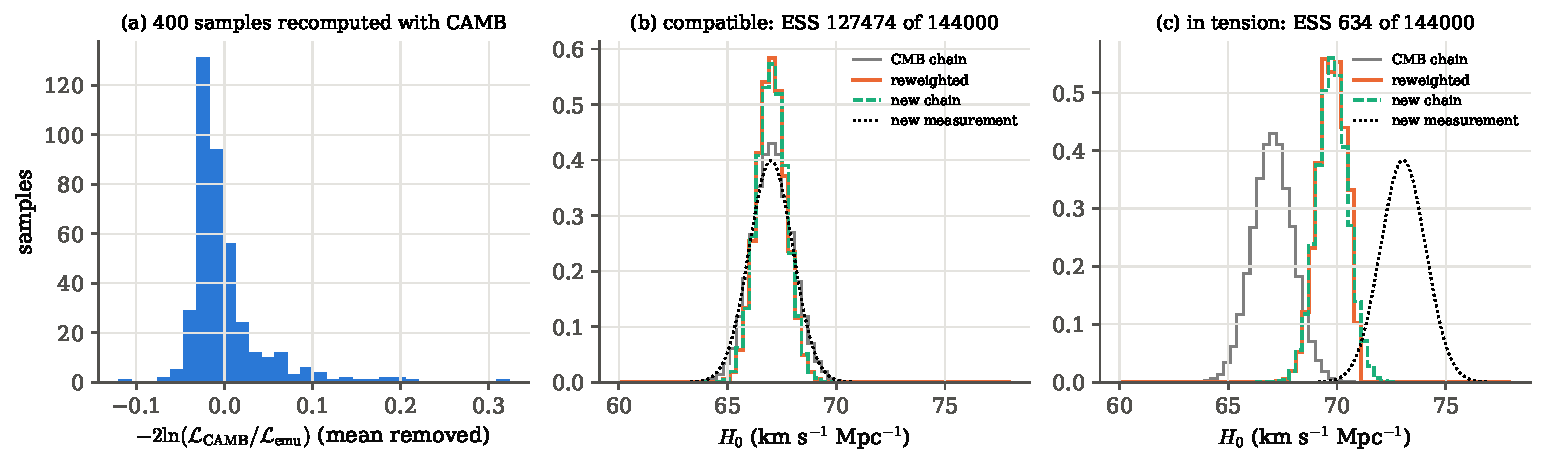
\includegraphics[width=\linewidth]{figures/ch09/importance.pdf}
\caption{Importance sampling a six-parameter CMB chain. (a) $-2\ln(\Like_{\rm CAMB}/\Like_{\rm emu})$ at 400 random samples: a
spread of a few hundredths, so the emulator chain needs no correction. (b) Adding a compatible $H_0$ measurement (dotted):
the reweighted chain (red) and a new chain (dashed) agree. (c) Adding a measurement in tension: only 0.4 per cent of the
samples carry weight, and the reweighted histogram is noisy and too narrow.}
\label{9c:fig:importance}
\end{figure}

\subsection{The research pipeline, stage by stage}
\label{9c:sec:pipeline}

A CMB temperature-and-polarization analysis of the Planck kind runs in seven stages
\cite{Planck2018V,Planck2018VI}. Each one produces something definite and is checked in a definite way; the laptop
counterpart of every stage is drawn in \cref{9c:fig:pipeline} and its cost is tabulated after it.
\begin{enumerate}[itemsep=2pt]
  \item \emph{Data products.} Maps at several frequencies (for Planck's high-$\ell$ likelihood, 100, 143 and 217\,GHz),
        split into halves of the mission so that cross-spectra have no noise bias; a mask for each frequency (Galactic
        and point sources); beam window functions; and simulations: 1000 sky realisations and 300 end-to-end
        simulations of the full instrument and processing (FFP10).
  \item \emph{Spectra and covariance.} Cross-spectra of the half-mission maps for every frequency pair, corrected for the
        mask by a MASTER-type deconvolution, binned (\cref{ch:08}); their covariance computed analytically for a fiducial
        model and corrected with simulations.
  \item \emph{Likelihood.} A hybrid: below $\ell=30$, the Blackwell--Rao temperature likelihood from Gibbs samples of the
        sky and a simulation-based polarization likelihood (lowE); above, the Gaussian of \cref{9c:sec:hl} with the
        fiducial covariance, and a model of foregrounds and calibrations with about fifteen nuisance parameters for
        temperature alone.
  \item \emph{Theory.} A Boltzmann code (CAMB or CLASS) called by the sampler for each proposed cosmology, with the
        nuisance parameters updated more often than the cosmological ones because they are cheap
        \cite{LewisBridle2002}.
  \item \emph{Sampling.} Metropolis--Hastings with a proposal covariance learned from earlier runs, several chains, and a
        stopping rule such as $\hat R-1<0.01$; a nested sampler when the evidence is needed. The codes are CosmoMC
        \cite{LewisBridle2002}, its successor Cobaya \cite{Torrado2021}, and MontePython \cite{Audren2013}.
  \item \emph{Products.} The chains themselves, with tables of marginal means and limits and triangle plots made by
        \pyname{getdist} \cite{Lewis2019GetDist}, and the parameter covariance, which is the file we compared with in
        \cref{9c:sec:planck}.
  \item \emph{Checks.} The pipeline is run on simulations with known inputs and must recover them on average (the
        300 FFP10 simulations); independent likelihood codes (Plik and CamSpec) must agree; results from different
        multipole ranges and frequency combinations must be consistent; null spectra must be compatible with noise;
        and importance sampling adds other data (CMB lensing, BAO) or checks the accuracy settings of the Boltzmann code.
\end{enumerate}

\begin{inpractice}[verification and research]
The straight line, the decaying source and the noiseless full sky were \emph{verifications}: the posterior was known
exactly (a Gaussian, a grid, a Student $t$, an exact likelihood) and the chain had to reproduce it, which it did to the
precision its effective sample size allows. The masked sky and the six-parameter Planck-like run are the \emph{research}
mode: no closed-form posterior exists, the covariance comes from simulations, and the chain with its diagnostics is the
instrument that produces the constraint. In real analyses the loop is exactly this one, with a Boltzmann code in place of
the emulator: CosmoMC and Cobaya \cite{LewisBridle2002,Torrado2021} and MontePython \cite{Audren2013} propose a cosmology,
call CAMB or CLASS, evaluate the Planck likelihood code, and accept or reject with the Metropolis rule; the chains are
analysed with \pyname{getdist}. Fisher forecasts (\cref{ch:10}) are checked against such chains, and the same machinery,
fed with simulated covariances of new summaries, will constrain parameters with topological statistics in \cref{ch:12}.
\end{inpractice}

\begin{figure}[htbp]
\centering
\begin{tikzpicture}[font=\small,
  st/.style={draw=accent,thick,rounded corners=2pt,fill=ideabg,align=center,text width=4.1cm,minimum height=0.9cm,inner sep=3pt},
  lt/.style={draw=black!40,rounded corners=2pt,fill=white,align=left,text width=5.6cm,minimum height=0.9cm,inner sep=3pt,font=\footnotesize}]
  \foreach \i/\a/\b in {
    0/{data: maps, splits, masks,\\beams, simulations}/{one simulated sky ($N_{\rm side}=256$) or a $\chi^2$-drawn spectrum; 2000 Gaussian simulations},
    1/{spectra and covariance}/{MASTER bandpowers, one channel; covariance from simulations with the Hartlap factor},
    2/{likelihood}/{exact full-sky form with $\fsky$, or Gaussian with fixed covariance; $\tau$ prior for lowE},
    3/{theory $\Cell(\params)$}/{Taylor emulator in $\ln\Cell$ (73 CAMB calls), validated to $\Delta\chi^2<0.1$},
    4/{sampler and diagnostics}/{\pyname{lib_mcmc9c}: 4 chains, $\hat R$, $\tau$, ESS; \pyname{emcee}, \pyname{getdist} cross-checks},
    5/{checks and extensions}/{500 skies for bias and coverage; importance sampling with CAMB and with $H_0$}}{
    \node[st] (s\i) at (0,-1.35*\i) {\a};
    \node[lt] (l\i) at (5.4,-1.35*\i) {\b};
    \draw[black!35,dashed] (s\i.east) -- (l\i.west);
  }
  \foreach \i [evaluate=\i as \j using int(\i+1)] in {0,...,4}{\draw[->,thick] (s\i) -- (s\j);}
  \node[font=\footnotesize\bfseries] at (0,0.9) {research stage};
  \node[font=\footnotesize\bfseries] at (5.4,0.9) {laptop version};
\end{tikzpicture}
\caption{The stages of a CMB parameter analysis (left) and the reduced version run on a laptop (right). The
statistics, the sampler and the diagnostics are the same; the data, the theory code and the size of the simulations
are reduced.}
\label{9c:fig:pipeline}
\end{figure}

\paragraph{What each laptop reduction costs.} Every reduction trades something for speed, as the table shows.
\begin{center}
\small
\renewcommand{\arraystretch}{1.15}
\begin{tabularx}{\linewidth}{@{}>{\raggedright\arraybackslash}p{3.3cm}>{\raggedright\arraybackslash}X>{\raggedright\arraybackslash}X@{}}
\toprule
our choice & research version & cost of the reduction\\\midrule
Taylor emulator, 73 CAMB calls & Boltzmann code at every step, or a neural emulator trained over the whole prior & valid only within a few $\sigma$ of the fiducial model\\
one simulated $\chi^2$ spectrum, $\fsky$ mode count & real cut-sky cross-spectra at three frequencies with a calibrated covariance & no mode coupling or foregrounds: $\sigma(n_s)$ about 7 per cent too small\\
temperature only, Gaussian prior on $\tau$ & TT, TE, EE, lensing; a non-Gaussian lowE likelihood & weaker constraints; a symmetric $\tau$ posterior\\
no nuisance parameters & about fifteen foreground and calibration parameters marginalised & widths and correlations slightly optimistic\\
toy sky: $N_{\rm side}=256$, $\ell\le601$, 2000 Gaussian simulations & $N_{\rm side}=2048$, $\ell\le2500$, 300 end-to-end plus 1000 sky simulations & fewer modes; covariance noise of order $\sqrt{2/n}$ on each element\\
chains of $4\times(2$--$4)\times10^4$ steps in seconds & chains of $10^5$ or more steps, days on a cluster with a Boltzmann code & none at the level of the diagnostics shown\\
importance check on 400 samples & reweighting the full chain in parallel & a check of the bulk, not of the far tails\\
\bottomrule
\end{tabularx}
\end{center}

\begin{recap}
\begin{itemize}[itemsep=1pt,leftmargin=1.2em]
  \item For a linear model with Gaussian errors the posterior is exactly Gaussian, with mean the weighted least-squares fit
        and covariance $(\mathbf A\T\mathbf W\mathbf A)^{-1}$, the Fisher matrix; the chain reproduces it, as does \pyname{emcee}.
  \item A column of a chain is a sample of that parameter's marginal: marginalising a nuisance parameter means ignoring
        its column. The marginal is wider than the slice at the best fit by $1/\sqrt{1-\rho^2}$.
  \item Published error bars depend on the noise model: Padilla et al.'s straight-line widths are those of one unknown
        common $\sigma$ (a Student-$t$ posterior), not of the stated errors.
  \item Slope and intercept correlate as $-\bar x_w/\sqrt{\overline{x^2}_w}$; centring $x$ (or choosing a pivot) removes the
        correlation and speeds the chain by orders of magnitude.
  \item A nonlinear model gives a skewed posterior that the Laplace (peak Gaussian) approximation misses and the chain
        does not. An unknown noise level, integrated out, turns $e^{-\chi^2/2}$ into $(\chi^2)^{-N/2}$; sampling it and ignoring
        its column gives the same marginal. Fixing it at a wrong value gives wrong widths without warning.
  \item Hyperparameters with prior $e^{-\alpha}$ give $(\chi^2_k+2)^{-(n_k/2+1)}$ per data set and let a posterior follow the
        consistent data; the Bayes factor is a ratio of integrals, not of likelihoods at a point. Multimodal posteriors
        defeat chains that never cross between modes.
  \item On the full sky the CMB likelihood is exact: $-2\ln\Like=\sum_\ell(2\ell+1)[\Chat/\Cell+\ln\Cell]$, with $\Cell\to T^2_\ell\Cell+N_\ell$
        for beam and noise and $2\ell+1\to(2\ell+1)\fsky$ for a partial sky; it is skewed at low $\ell$.
  \item Gaussian approximations differ from it in the cubic term in $\Chat/\Cell-1$. $\Like_Q$ biases a spectrum up by
        $0.9/\ell$ in bins of ten and $n_s$ by more than one standard deviation; a fixed fiducial covariance ($\Like_f$, Planck's
        choice) is unbiased in the ideal case. Hamimeche and Lewis's Fig.~1 is reproduced to a few per cent.
  \item An emulator in $\ln\Cell$ is natural ($\ln A_s$ and $\tau$ enter linearly, $n_s$ almost) and must be validated with
        $\Delta\chi^2=\sum\frac\nu2[\delta C/(C+N)]^2\ll1$: first order for $(\ln A_s,n_s)$, second order for six parameters.
  \item The amplitude and tilt are a straight-line fit in $x_\ell=\langle\ln k/k_*\rangle_\ell$; the sign of their correlation is the
        side of the pivot the data lie on.
  \item A Planck-like TT+lowE simulation reproduces Planck 2018's widths to ten per cent with six parameters free;
        $\sigma(\ln A_s)\approx2\sigma_\tau$ because TT measures only $A_se^{-2\tau}$; fixing the other parameters makes the
        amplitude nine times and the tilt twice too precise.
  \item Importance sampling reweights a chain by $\Like_{\rm new}/\Like_{\rm old}$; the effective sample size
        $(\sum w)^2/\sum w^2$ shows when it works (compatible data, accurate approximations) and when it fails (tension).
\end{itemize}
\end{recap}

\subsection*{Reading the literature}
\label{9c:sec:reading-list}

\begin{itemize}[itemsep=2pt,leftmargin=1.2em]
  \item \textbf{Markov chains and MCMC, textbook level.} Wasserman, \emph{All of Statistics}, Chapters~23 (Markov chains)
        and~24 (Metropolis--Hastings, Gibbs) \mainref{pp.~381--420}; Kruschke, \emph{Doing Bayesian Data Analysis},
        Chapters~7 (MCMC with the island-hopping politician, diagnostics) and~17 (regression, centring, posterior
        predictive lines) \srcref{Kruschke}{Chs.~7, 8, 17}; Lambert, \emph{A Student's Guide to Bayesian Statistics},
        Chapters~12--14 on the typical set, $\hat R$ and effective sample size \srcref{Lambert}{Chs.~12--14}.
  \item \textbf{The original algorithms.} Metropolis et al.\ on the canonical ensemble \cite{Metropolis1953}; Hastings on
        asymmetric proposals \cite{Hastings1970}; Peskun on the optimality of the Metropolis acceptance \cite{Peskun1973};
        Roberts, Gelman and Gilks on the $2.38/\sqrt d$ scaling \cite{RobertsGelmanGilks1997}; Gelman and Rubin, and Brooks
        and Gelman, on multiple chains \cite{GelmanRubin1992,BrooksGelman1998}; Sokal on autocorrelation times
        \cite{Sokal1997}; Geman and Geman on Gibbs sampling \cite{GemanGeman1984}; Duane et al.\ and Neal on Hamiltonian
        Monte Carlo \cite{Duane1987,Neal2011}; Goodman and Weare, and Foreman-Mackey et al.\ (\pyname{emcee}), on
        affine-invariant ensembles \cite{GoodmanWeare2010,ForemanMackey2013}.
  \item \textbf{MCMC in cosmology.} Lewis and Bridle on CosmoMC, proposal covariances, fast and slow parameters and
        importance sampling \cite{LewisBridle2002}, and their chapter in Hobson et al., \emph{Bayesian Methods in Cosmology}
        \srcref{HobsonBMC}{Ch.~3}; Dunkley et al.\ on convergence and efficiency of cosmological chains \cite{Dunkley2005};
        Padilla et al.\ for a worked tour from coins to straight lines to cosmology \cite{Padilla2019}; Torrado and Lewis on
        Cobaya \cite{Torrado2021}; Audren et al.\ on MontePython \cite{Audren2013}; Lewis on \pyname{getdist}
        \cite{Lewis2019GetDist}; Spurio Mancini et al.\ on neural emulators \cite{SpurioMancini2022}.
  \item \textbf{CMB likelihoods.} Hobson et al., Chapter~10, on the CMB as a hierarchical model, from maps to spectra to
        parameters \srcref{HobsonBMC}{pp.~237--240}; Hamimeche and Lewis on the exact full-sky likelihood and its
        approximations \cite{HamimecheLewis2008}; Bond, Jaffe and Knox on offset log-normal forms \cite{BondJaffeKnox2000};
        Verde et al.\ on the WMAP likelihood \cite{Verde2003}; Chu et al.\ on the Blackwell--Rao estimator \cite{Chu2005};
        Hivon et al.\ on MASTER \cite{Hivon2002}; Hartlap et al.\ on inverting simulated covariances \cite{Hartlap2007}.
  \item \textbf{Planck.} Planck 2018 V on the likelihoods \cite{Planck2018V} and VI on the cosmological parameters
        \cite{Planck2018VI}; Planck 2018 I for the instrument \cite{Planck2018I}; CAMB \cite{CAMB2000}.
\end{itemize}

\section*{Chapter summary}
\addcontentsline{toc}{section}{Chapter summary}
\label{9c:sec:summary}

A posterior that can be evaluated point by point but not integrated is known only in principle. A Markov chain turns
it into a sample. The chain is a random walker that remembers only where it is; if the target density is stationary
for its hopping rule, the walker forgets where it started and its time averages converge to averages over the target.
Metropolis--Hastings supplies such a rule for any target: propose a step, accept it with the ratio of densities, and
repeat the current point on refusal. Without the accept--reject step the walker would diffuse forever and sample
nothing; the step is the bias that makes it linger where the probability is high, and because only ratios enter, the
evidence never has to be computed. A finite chain is trusted only after its diagnostics: burn-in, several chains that
agree ($\hat R$), and the autocorrelation time that converts $N$ steps into $N/\tau$ independent ones. Then every
marginal is a histogram of a column, and every constraint is read off. On a straight line, a decaying source and a
full-sky spectrum the chain reproduces exact answers; on a masked sky and a six-parameter Planck-like spectrum it is
the instrument that produces them, reproducing Planck's published widths once the same parameters are left free. In
the pipeline
\[
  \text{physical model}\to\text{field}\to\text{summary }S\to P(S\given\theta)\to
  \boxed{\text{infer physics}},
\]
Markov chain Monte Carlo is the last arrow: it turns the sampling distribution of \cref{ch:07,ch:08} into posterior constraints.
\Cref{ch:10} gives the fast Gaussian forecast that the chains check, \cref{ch:12} applies the same chains to
topological summaries, and \cref{ch:13} runs them on Planck data.

\begin{center}
\small
\renewcommand{\arraystretch}{1.15}
\begin{tabularx}{\linewidth}{@{}>{\raggedright\arraybackslash}p{3.3cm}
                               >{\raggedright\arraybackslash}X
                               >{\raggedright\arraybackslash}p{2.3cm}@{}}
\toprule
\multicolumn{3}{@{}l}{\textbf{Markov chains}}\\
concept & operational meaning & used later in\\\midrule
Markov chain & next state drawn from $p(x,\cdot)$ depending only on the current state; rows of $P$ are pmfs & \cref{ch:12,ch:13}\\
stationary distribution & $\pi P=\pi$; probability flowing in balances flowing out & \cref{ch:10,ch:13}\\
detailed balance & $\pi_ip_{ij}=\pi_jp_{ji}$; sufficient for stationarity; no net currents & \cref{ch:13}\\
irreducible, aperiodic, positive recurrent & every state reachable, no cycles, finite return time: the chain converges & \cref{ch:13}\\
convergence (forgetting) & $\norm{p_t-\pi}_{\rm TV}\sim\abs{\lambda_2}^t$; any start is forgotten & \cref{ch:13}\\
ergodic theorem & time average along one chain $\to$ average over $\pi$ & \cref{ch:10,ch:12,ch:13}\\
autocorrelation time & $\tau=1+2\sum\rho_k$; variance of a chain mean $\sigma^2\tau/N$ & \cref{ch:12,ch:13}\\
free random walk & spreads as $\sqrt t$, no stationary law: the walker MH must bias & \cref{ch:11}\\
\bottomrule
\end{tabularx}
\end{center}

\begin{center}
\small
\renewcommand{\arraystretch}{1.15}
\begin{tabularx}{\linewidth}{@{}>{\raggedright\arraybackslash}p{3.3cm}
                               >{\raggedright\arraybackslash}X
                               >{\raggedright\arraybackslash}p{2.3cm}@{}}
\toprule
\multicolumn{3}{@{}l}{\textbf{The biased random walker}}\\
concept & operational meaning & used later in\\\midrule
Metropolis--Hastings & propose $y\sim q(y\given x)$, accept with $\min(1,f(y)q(x\given y)/f(x)q(y\given x))$, else repeat $x$ & \cref{ch:12,ch:13,ch:11}\\
only ratios & evidence and partition function cancel; work with $\ln f$ & \cref{ch:13}\\
Hastings factor & Jacobian of an asymmetric proposal; omitting it samples the wrong target & \cref{ch:13}\\
step size & round step $2.38/\sqrt D$ target widths, acceptance $\approx0.23$; shape the proposal by the covariance & \cref{ch:10,ch:13}\\
burn-in & cut where $\ln p$ settles near $\ln p_{\max}-D/2$, not at the peak & \cref{ch:13}\\
ESS, MCSE & $N/\tau$ effective draws; Monte Carlo error $\mathrm{SD}\sqrt{\tau/N}$; thinning never helps & \cref{ch:12,ch:13}\\
$\hat R$ & several overdispersed chains; $\sqrt{\hat V/W}\to1$; blind to modes no chain found & \cref{ch:13}\\
start vs prior & the start is forgotten, the prior is part of the target & \cref{ch:10,ch:13}\\
canonical ensemble & Metropolis samples $e^{-H/kT}$; MCMC time is not physical time & \cref{ch:12}\\
Gibbs, HMC, ensembles & always-accepted conditional moves; Hamiltonian flights; affine-invariant walkers (\pyname{emcee}) & \cref{ch:13,ch:11}\\
\bottomrule
\end{tabularx}
\end{center}

\begin{center}
\small
\renewcommand{\arraystretch}{1.15}
\begin{tabularx}{\linewidth}{@{}>{\raggedright\arraybackslash}p{3.3cm}
                               >{\raggedright\arraybackslash}X
                               >{\raggedright\arraybackslash}p{2.3cm}@{}}
\toprule
\multicolumn{3}{@{}l}{\textbf{MCMC at work}}\\
concept & operational meaning & used later in\\\midrule
marginal from a chain & histogram one column, ignore the others & \cref{ch:10,ch:12,ch:13}\\
linear-Gaussian posterior & exact Gaussian with covariance $(\mathbf A\T\mathbf W\mathbf A)^{-1}$ = inverse Fisher matrix & \cref{ch:10}\\
centring, pivot & move the origin to the data's weighted centre to decorrelate parameters & \cref{ch:10,ch:13}\\
Laplace approximation & Gaussian from the curvature at the peak; misses skewness of nonlinear models & \cref{ch:10}\\
nuisance noise level & integrate out ($(\chi^2)^{-N/2}$) or sample and ignore; never fix at a guess & \cref{ch:13,ch:11}\\
hyperparameters & one marginalised weight per data set, $(\chi^2_k+2)^{-(n_k/2+1)}$; Bayes factor by integration & \cref{ch:11}\\
exact full-sky $\Cell$ likelihood & $\sum(2\ell+1)[\Chat/\Cell+\ln\Cell]$; $\Cell\to T^2\Cell+N$; $\nu\to(2\ell+1)\fsky$ & \cref{ch:10,ch:13}\\
Gaussian $\Cell$ likelihoods & fixed fiducial covariance unbiased; model-dependent variance ($\Like_Q$) biases $n_s$ by $\sim1\sigma$ & \cref{ch:13}\\
emulator & Taylor series of $\ln\Cell$; validate by $\Delta\chi^2=\sum\frac\nu2(\delta C/(C+N))^2\ll1$ on the posterior & \cref{ch:10,ch:13}\\
triangle plot & 1-D and 2-D marginals; 68/95 per cent levels by sorted cells; $\Delta\chi^2=2.30$, $6.18$ in 2-D & \cref{ch:10,ch:12,ch:13}\\
$A_se^{-2\tau}$ degeneracy & TT measures $\ln A_s-2\tau$; $\sigma(\ln A_s)\approx2\sigma_\tau$ & \cref{ch:10,ch:13}\\
importance sampling & reweight by $\Like_{\rm new}/\Like_{\rm old}$; $N_{\rm eff}=(\sum w)^2/\sum w^2$; fails for data in tension & \cref{ch:13,ch:11}\\
\bottomrule
\end{tabularx}
\end{center}
  